%%
%% Slides for Applications of Artificial Intelligence course
%% Department of Informatics and Telematics,
%% Harokopio University of Athens, Greece.
%%
%% Author: Christos Diou

%%
%% Beamer presentation preamble template for Applications of Artificial
%% Intelligence course
%% Department of Informatics and Telematics,
%% Harokopio University of Athens, Greece.
%%
%% Author: Christos Diou

\documentclass[article,aspectratio=169]{beamer}

%%%%%%%%%%%% Preamble %%%%%%%%%%%%

\usefonttheme[onlysmall]{structurebold}

%% Math stuff
\usepackage{amssymb}
\usepackage{amsmath}
\usepackage{amsfonts}
\usepackage{amsthm}
\usepackage{bm}
\usepackage{bbold}
\newcommand{\mathbbm}[1]{\text{\usefont{U}{bbm}{m}{n}#1}} % from mathbbm.sty


% Frequently used vectors
\newcommand{\Vu}{\mathbf{u}}
\newcommand{\Vh}{\mathbf{h}}
\newcommand{\Vv}{\mathbf{v}}
\newcommand{\Vw}{\mathbf{w}}
\newcommand{\Vb}{\mathbf{b}}
\newcommand{\Vx}{\mathbf{x}}
\newcommand{\Vy}{\mathbf{y}}
\newcommand{\Vz}{\mathbf{z}}
\newcommand{\Vf}{\mathbf{f}}
\newcommand{\VC}{\mathbf{C}}
\newcommand{\VD}{\mathbf{D}}
\newcommand{\VX}{\mathbf{X}}
\newcommand{\VS}{\mathbf{S}}
\newcommand{\VW}{\mathbf{W}}
\newcommand{\VV}{\mathbf{V}}
\newcommand{\VU}{\mathbf{U}}
\newcommand{\Vth}{\bm{\theta}}
\newcommand{\pmodel}{p_{\text{model}}}
\newcommand{\pdata}{\hat{p}_{\text{data}}}
\newcommand{\thetab}{\boldsymbol{\theta}}
\newcommand{\xb}{\boldsymbol{x}}

% argmin and argmax
\DeclareMathOperator*{\argmax}{arg\,max}
\DeclareMathOperator*{\argmin}{arg\,min}

%% Graphics
\usepackage{graphicx}
\graphicspath{{logos/}{figures/}}
\DeclareGraphicsExtensions{.jpg,.png,.jpeg,.pdf,.tiff}
\usepackage{tikz}
\usetikzlibrary{matrix,positioning,arrows.meta,arrows,fit,backgrounds,decorations.pathreplacing}

\tikzset{
  mymat/.style={ matrix of math nodes, text height=2.5ex, text
    depth=0.75ex, text width=6.00ex, align=center, column
    sep=-\pgflinewidth, nodes={minimum height=5.0ex}
  },
  mymats/.style={ mymat, nodes={draw,fill=#1}
  },
  mymat2/.style={
    matrix of math nodes, text height=1.0ex, text depth=0.0ex, minimum
    width=5ex, % text
    width=7.00ex, align=center, column sep=-\pgflinewidth
  },
}
\usepackage{tikzsymbols}
\usepackage{pgfpages}
\usepackage{pgfplots}
%\usepackage[active,tightpage,pdftex]{preview}
%\PreviewEnvironment{tikzpicture}
\usepackage{multimedia}

% \usetikzlibrary{arrows,shapes}
% \tikzstyle{every picture}+=[remember picture]

\usepackage{xcolor}

%% Fonts
\usepackage[cm-default,no-math]{fontspec}
\setmonofont{FreeMono}
% \setmainfont[Mapping=tex-text,ItalicFont={Minion Pro Italic},BoldFont={Minion
% Pro Bold},BoldItalicFont={Minion Pro Bold Italic}]{GFS Elpis}
\setmainfont{PF Square Sans Pro}
\setsansfont{PF Square Sans Pro}
% \setsansfont[Mapping=tex-text,ItalicFont={Minion Pro Italic},BoldFont={Minion Pro Bold},BoldItalicFont={Minion Pro Bold Italic}]{GFS Elpis}
\usepackage{xgreek}
\usepackage{xunicode}
\usepackage{xltxtra}

%% Algorithms
\usepackage{algorithm}
\floatname{algorithm}{Αλγόριθμος}
%\usepackage[ruled]{algorithm2e}
%\usepackage{algpseudocode}
%\usepackage{algc}
\usepackage{algorithmic}
%\algsetup{linenosize=\tiny}

% Code
\definecolor{bg}{rgb}{0.95,0.95,0.95}
\definecolor{lightred}{rgb}{0.95,0.85,0.85}
\makeatletter
\newcommand{\currentfontsize}{\fontsize{\f@size}{\f@baselineskip}\selectfont}
\makeatother

%% Others
\usepackage{multirow}
\usepackage{hyperref}
\hypersetup{
  colorlinks=true,
  linkcolor=blue,
  filecolor=magenta,      
  urlcolor=cyan,
}
\urlstyle{same}
\usepackage[absolute,overlay]{textpos}
\usepackage{array}

\newcommand{\obf}[1]{{\color{orange} \textbf{#1}}}
\newcommand{\orange}[1]{{\color{orange} #1}}
\newcommand{\rbf}[1]{{\color{red} \textbf{#1}}}
\newcommand{\red}[1]{{\color{red} #1}}

%\usepackage{concmath}

%% Beamer options

%\usefonttheme[onlymath]{serif}
\usefonttheme{professionalfonts}
%\usepackage[texcoord,grid,gridunit=mm,gridcolor=red!10,subgridcolor=green!10]{eso-pic}
%\usepackage[texcoord,gridunit=mm,gridcolor=red!10,subgridcolor=green!10]{eso-pic}
\setbeamertemplate{navigation symbols}{}%remove navigation symbols
\setbeamertemplate{page number in head/foot}[pagenumber]
\setbeamercolor{page number in head/foot}{fg=gray}
\setbeamertemplate{footline}[frame number]
\setbeamertemplate{frametitle}[default][center]
%\setbeameroption{show notes on second screen}
%\setbeameroption{show notes}
\setbeamerfont{note page}{size=\scriptsize}
\setbeamertemplate{note page}[plain]
\setbeamertemplate{itemize items}[circle]
\setbeamertemplate{enumerate items}[default]

% For faster compile on development
% \includeonlyframes{current}

%% New commands
\newcommand\FrameText[1]{%
  \begin{textblock*}{\paperwidth}(0pt,.95\textheight)
    \hfill #1 \hspace{2em}
    % \raggedright #1\hspace{.5em}
\end{textblock*}}

\newcommand\FrameTextTop[1]{%
  \begin{textblock*}{\paperwidth}(0pt,.05\textheight)
    \hfill #1 \hspace{2em}
    % \raggedright #1\hspace{.5em}
\end{textblock*}}

%% \titlegraphic{
%%   \begin{textblock*}{0.95\paperwidth}(2mm,1mm)
%%     \adjustbox{valign=c}{
\includegraphics[width=0.31\linewidth,keepaspectratio]{hua_logo}}
%%     \hfill
%%     \adjustbox{valign=c}{
\includegraphics[width=0.15\linewidth,keepaspectratio]{dit_hua_logo}}
%%   \end{textblock*}
%% }
\titlegraphic{
  \begin{textblock*}{0.95\paperwidth}(2mm,1mm)
    
\includegraphics[width=0.31\linewidth,keepaspectratio]{hua_logo}
    \hfill
    
\includegraphics[width=0.15\linewidth,keepaspectratio]{dit_hua_logo}
  \end{textblock*}
}

\author{Χρήστος Δίου}
\institute{Τμήμα Πληροφορικής και Τηλεματικής\\
  Χαροκόπειο Πανεπιστήμιο}
\date{\small ΕΚΕΤΑ-ΙΠΤΗΛ 4/1/2022}


%%%%%%%%%%%% Main content start %%%%%%%%%%%%


%% \Large IML and DALE: Introduction to Interpretable Machine
%% Learning \footnote{Some ideas and content from  Christoph Molnar's book, ``Interpretable Machine Learning book'',
%% \url{https://christophm.github.io/interpretable-ml-book/}} and Differential
%% Accumulated Local Effects\footnote{based on work with colleagues V. Gkolemis
%% and T. Dalamagas, \url{https://arxiv.org/abs/2210.04542}}

\title{\Large{IML and DALE: Introduction to Interpretable Machine
    Learning and Differential Accumulated Local Effects}}

\AtBeginSection[]{
  \begin{frame}{Contents}
    \small \tableofcontents[currentsection, hideothersubsections]
  \end{frame} 
}

\begin{document}

\frame{\titlepage}

% Use label=current to render only one slide

\section{Introduction}

\begin{frame}[plain,c]
  \Large Short introduction to interpretable machine learning \footnote{Some
  ideas and content from Christoph Molnar's book, ``Interpretable Machine Learning'' (IML book),
  \url{https://christophm.github.io/interpretable-ml-book/}}
\end{frame}

\begin{frame}
  \frametitle{Hypothetical (?) scenarios}

  \begin{itemize}
  \item<1-> The computer vision subsystem of an autonomous vehicle leads the
    vehicle to take a left turn, in front of a car moving in the opposite direction\footnote{\url{https://www.theguardian.com/technology/2022/dec/22/tesla-crash-full-self-driving-mode-san-francisco}}
  \item<2-> The credit assessment system leads to the rejection of an
    application for a loan - the client suspects racial bias\footnote{\url{https://www.technologyreview.com/2021/06/17/1026519/racial-bias-noisy-data-credit-scores-mortgage-loans-fairness-machine-learning/}}
  \item<3-> A model that assesses the risk of future criminal offenses (and
    used for decisions on parole sentences) is biased against black
    prisoners\footnote{\url{https://www.propublica.org/article/machine-bias-risk-assessments-in-criminal-sentencing}}
  \end{itemize}

\end{frame}

\begin{frame}
  \frametitle{Questions}
  \begin{itemize}
  \item Why did a model make a specific decision?
  \item What could we change so that the model will make a different decision?
  \item Can we summarize and predict the model's behavior?
  \end{itemize}
\end{frame}

\begin{frame}
  \frametitle{Interpretability of Machine Learning Models}
  Qualitative definitions:
  \begin{itemize}
  \item ``Interpretability is the degree to which a human can understand the
    cause of a decision'' \footnote{Miller, Tim. ``Explanation in artificial
    intelligence: Insights from the social sciences.'' arXiv Preprint
    arXiv:1706.07269. (2017)}
  \item ``Interpretability is the degree to which a human can consistently
    predict the model’s result''\footnote{Kim, Been, Rajiv Khanna, and
    Oluwasanmi O. Koyejo. ``Examples are not enough, learn to criticize!
    Criticism for interpretability.'' Advances in Neural Information Processing
    Systems (2016).} 
  \item ``Extraction of relevant knowledge from a machine-learning model
    concerning relationships either contained in data or learned by the
    model''\footnote{Murdoch, W. J., Singh, C., Kumbier, K., Abbasi-Asl, R. and
    Yu, B. ``Definitions, methods, and applications in interpretable machine
    learning.'' Proceedings of the National Academy of Sciences, 116(44),
    22071-22080. (2019)} 
  \end{itemize}
\end{frame}

\begin{frame}
  \frametitle{Generalization}
  \begin{onlyenv}<1>
    To get some intuition, consider a process that produces output
    $y$ for scalar input $x$
    \begin{center}
      \scalebox{0.5}{
        %% Creator: Matplotlib, PGF backend
%%
%% To include the figure in your LaTeX document, write
%%   \input{<filename>.pgf}
%%
%% Make sure the required packages are loaded in your preamble
%%   \usepackage{pgf}
%%
%% Figures using additional raster images can only be included by \input if
%% they are in the same directory as the main LaTeX file. For loading figures
%% from other directories you can use the `import` package
%%   \usepackage{import}
%% and then include the figures with
%%   \import{<path to file>}{<filename>.pgf}
%%
%% Matplotlib used the following preamble
%%   \usepackage{fontspec}
%%   \setmainfont{DejaVuSerif.ttf}[Path=/home/diou/miniconda3/envs/ml/lib/python3.8/site-packages/matplotlib/mpl-data/fonts/ttf/]
%%   \setsansfont{DejaVuSans.ttf}[Path=/home/diou/miniconda3/envs/ml/lib/python3.8/site-packages/matplotlib/mpl-data/fonts/ttf/]
%%   \setmonofont{DejaVuSansMono.ttf}[Path=/home/diou/miniconda3/envs/ml/lib/python3.8/site-packages/matplotlib/mpl-data/fonts/ttf/]
%%
\begingroup%
\makeatletter%
\begin{pgfpicture}%
\pgfpathrectangle{\pgfpointorigin}{\pgfqpoint{6.400000in}{4.800000in}}%
\pgfusepath{use as bounding box, clip}%
\begin{pgfscope}%
\pgfsetbuttcap%
\pgfsetmiterjoin%
\definecolor{currentfill}{rgb}{1.000000,1.000000,1.000000}%
\pgfsetfillcolor{currentfill}%
\pgfsetlinewidth{0.000000pt}%
\definecolor{currentstroke}{rgb}{1.000000,1.000000,1.000000}%
\pgfsetstrokecolor{currentstroke}%
\pgfsetdash{}{0pt}%
\pgfpathmoveto{\pgfqpoint{0.000000in}{0.000000in}}%
\pgfpathlineto{\pgfqpoint{6.400000in}{0.000000in}}%
\pgfpathlineto{\pgfqpoint{6.400000in}{4.800000in}}%
\pgfpathlineto{\pgfqpoint{0.000000in}{4.800000in}}%
\pgfpathclose%
\pgfusepath{fill}%
\end{pgfscope}%
\begin{pgfscope}%
\pgfsetbuttcap%
\pgfsetmiterjoin%
\definecolor{currentfill}{rgb}{1.000000,1.000000,1.000000}%
\pgfsetfillcolor{currentfill}%
\pgfsetlinewidth{0.000000pt}%
\definecolor{currentstroke}{rgb}{0.000000,0.000000,0.000000}%
\pgfsetstrokecolor{currentstroke}%
\pgfsetstrokeopacity{0.000000}%
\pgfsetdash{}{0pt}%
\pgfpathmoveto{\pgfqpoint{0.800000in}{0.528000in}}%
\pgfpathlineto{\pgfqpoint{5.760000in}{0.528000in}}%
\pgfpathlineto{\pgfqpoint{5.760000in}{4.224000in}}%
\pgfpathlineto{\pgfqpoint{0.800000in}{4.224000in}}%
\pgfpathclose%
\pgfusepath{fill}%
\end{pgfscope}%
\begin{pgfscope}%
\pgfpathrectangle{\pgfqpoint{0.800000in}{0.528000in}}{\pgfqpoint{4.960000in}{3.696000in}}%
\pgfusepath{clip}%
\pgfsetrectcap%
\pgfsetroundjoin%
\pgfsetlinewidth{0.803000pt}%
\definecolor{currentstroke}{rgb}{0.690196,0.690196,0.690196}%
\pgfsetstrokecolor{currentstroke}%
\pgfsetdash{}{0pt}%
\pgfpathmoveto{\pgfqpoint{1.025455in}{0.528000in}}%
\pgfpathlineto{\pgfqpoint{1.025455in}{4.224000in}}%
\pgfusepath{stroke}%
\end{pgfscope}%
\begin{pgfscope}%
\pgfsetbuttcap%
\pgfsetroundjoin%
\definecolor{currentfill}{rgb}{0.000000,0.000000,0.000000}%
\pgfsetfillcolor{currentfill}%
\pgfsetlinewidth{0.803000pt}%
\definecolor{currentstroke}{rgb}{0.000000,0.000000,0.000000}%
\pgfsetstrokecolor{currentstroke}%
\pgfsetdash{}{0pt}%
\pgfsys@defobject{currentmarker}{\pgfqpoint{0.000000in}{-0.048611in}}{\pgfqpoint{0.000000in}{0.000000in}}{%
\pgfpathmoveto{\pgfqpoint{0.000000in}{0.000000in}}%
\pgfpathlineto{\pgfqpoint{0.000000in}{-0.048611in}}%
\pgfusepath{stroke,fill}%
}%
\begin{pgfscope}%
\pgfsys@transformshift{1.025455in}{0.528000in}%
\pgfsys@useobject{currentmarker}{}%
\end{pgfscope}%
\end{pgfscope}%
\begin{pgfscope}%
\definecolor{textcolor}{rgb}{0.000000,0.000000,0.000000}%
\pgfsetstrokecolor{textcolor}%
\pgfsetfillcolor{textcolor}%
\pgftext[x=1.025455in,y=0.430778in,,top]{\color{textcolor}\sffamily\fontsize{10.000000}{12.000000}\selectfont 0.0}%
\end{pgfscope}%
\begin{pgfscope}%
\pgfpathrectangle{\pgfqpoint{0.800000in}{0.528000in}}{\pgfqpoint{4.960000in}{3.696000in}}%
\pgfusepath{clip}%
\pgfsetrectcap%
\pgfsetroundjoin%
\pgfsetlinewidth{0.803000pt}%
\definecolor{currentstroke}{rgb}{0.690196,0.690196,0.690196}%
\pgfsetstrokecolor{currentstroke}%
\pgfsetdash{}{0pt}%
\pgfpathmoveto{\pgfqpoint{1.927273in}{0.528000in}}%
\pgfpathlineto{\pgfqpoint{1.927273in}{4.224000in}}%
\pgfusepath{stroke}%
\end{pgfscope}%
\begin{pgfscope}%
\pgfsetbuttcap%
\pgfsetroundjoin%
\definecolor{currentfill}{rgb}{0.000000,0.000000,0.000000}%
\pgfsetfillcolor{currentfill}%
\pgfsetlinewidth{0.803000pt}%
\definecolor{currentstroke}{rgb}{0.000000,0.000000,0.000000}%
\pgfsetstrokecolor{currentstroke}%
\pgfsetdash{}{0pt}%
\pgfsys@defobject{currentmarker}{\pgfqpoint{0.000000in}{-0.048611in}}{\pgfqpoint{0.000000in}{0.000000in}}{%
\pgfpathmoveto{\pgfqpoint{0.000000in}{0.000000in}}%
\pgfpathlineto{\pgfqpoint{0.000000in}{-0.048611in}}%
\pgfusepath{stroke,fill}%
}%
\begin{pgfscope}%
\pgfsys@transformshift{1.927273in}{0.528000in}%
\pgfsys@useobject{currentmarker}{}%
\end{pgfscope}%
\end{pgfscope}%
\begin{pgfscope}%
\definecolor{textcolor}{rgb}{0.000000,0.000000,0.000000}%
\pgfsetstrokecolor{textcolor}%
\pgfsetfillcolor{textcolor}%
\pgftext[x=1.927273in,y=0.430778in,,top]{\color{textcolor}\sffamily\fontsize{10.000000}{12.000000}\selectfont 0.5}%
\end{pgfscope}%
\begin{pgfscope}%
\pgfpathrectangle{\pgfqpoint{0.800000in}{0.528000in}}{\pgfqpoint{4.960000in}{3.696000in}}%
\pgfusepath{clip}%
\pgfsetrectcap%
\pgfsetroundjoin%
\pgfsetlinewidth{0.803000pt}%
\definecolor{currentstroke}{rgb}{0.690196,0.690196,0.690196}%
\pgfsetstrokecolor{currentstroke}%
\pgfsetdash{}{0pt}%
\pgfpathmoveto{\pgfqpoint{2.829091in}{0.528000in}}%
\pgfpathlineto{\pgfqpoint{2.829091in}{4.224000in}}%
\pgfusepath{stroke}%
\end{pgfscope}%
\begin{pgfscope}%
\pgfsetbuttcap%
\pgfsetroundjoin%
\definecolor{currentfill}{rgb}{0.000000,0.000000,0.000000}%
\pgfsetfillcolor{currentfill}%
\pgfsetlinewidth{0.803000pt}%
\definecolor{currentstroke}{rgb}{0.000000,0.000000,0.000000}%
\pgfsetstrokecolor{currentstroke}%
\pgfsetdash{}{0pt}%
\pgfsys@defobject{currentmarker}{\pgfqpoint{0.000000in}{-0.048611in}}{\pgfqpoint{0.000000in}{0.000000in}}{%
\pgfpathmoveto{\pgfqpoint{0.000000in}{0.000000in}}%
\pgfpathlineto{\pgfqpoint{0.000000in}{-0.048611in}}%
\pgfusepath{stroke,fill}%
}%
\begin{pgfscope}%
\pgfsys@transformshift{2.829091in}{0.528000in}%
\pgfsys@useobject{currentmarker}{}%
\end{pgfscope}%
\end{pgfscope}%
\begin{pgfscope}%
\definecolor{textcolor}{rgb}{0.000000,0.000000,0.000000}%
\pgfsetstrokecolor{textcolor}%
\pgfsetfillcolor{textcolor}%
\pgftext[x=2.829091in,y=0.430778in,,top]{\color{textcolor}\sffamily\fontsize{10.000000}{12.000000}\selectfont 1.0}%
\end{pgfscope}%
\begin{pgfscope}%
\pgfpathrectangle{\pgfqpoint{0.800000in}{0.528000in}}{\pgfqpoint{4.960000in}{3.696000in}}%
\pgfusepath{clip}%
\pgfsetrectcap%
\pgfsetroundjoin%
\pgfsetlinewidth{0.803000pt}%
\definecolor{currentstroke}{rgb}{0.690196,0.690196,0.690196}%
\pgfsetstrokecolor{currentstroke}%
\pgfsetdash{}{0pt}%
\pgfpathmoveto{\pgfqpoint{3.730909in}{0.528000in}}%
\pgfpathlineto{\pgfqpoint{3.730909in}{4.224000in}}%
\pgfusepath{stroke}%
\end{pgfscope}%
\begin{pgfscope}%
\pgfsetbuttcap%
\pgfsetroundjoin%
\definecolor{currentfill}{rgb}{0.000000,0.000000,0.000000}%
\pgfsetfillcolor{currentfill}%
\pgfsetlinewidth{0.803000pt}%
\definecolor{currentstroke}{rgb}{0.000000,0.000000,0.000000}%
\pgfsetstrokecolor{currentstroke}%
\pgfsetdash{}{0pt}%
\pgfsys@defobject{currentmarker}{\pgfqpoint{0.000000in}{-0.048611in}}{\pgfqpoint{0.000000in}{0.000000in}}{%
\pgfpathmoveto{\pgfqpoint{0.000000in}{0.000000in}}%
\pgfpathlineto{\pgfqpoint{0.000000in}{-0.048611in}}%
\pgfusepath{stroke,fill}%
}%
\begin{pgfscope}%
\pgfsys@transformshift{3.730909in}{0.528000in}%
\pgfsys@useobject{currentmarker}{}%
\end{pgfscope}%
\end{pgfscope}%
\begin{pgfscope}%
\definecolor{textcolor}{rgb}{0.000000,0.000000,0.000000}%
\pgfsetstrokecolor{textcolor}%
\pgfsetfillcolor{textcolor}%
\pgftext[x=3.730909in,y=0.430778in,,top]{\color{textcolor}\sffamily\fontsize{10.000000}{12.000000}\selectfont 1.5}%
\end{pgfscope}%
\begin{pgfscope}%
\pgfpathrectangle{\pgfqpoint{0.800000in}{0.528000in}}{\pgfqpoint{4.960000in}{3.696000in}}%
\pgfusepath{clip}%
\pgfsetrectcap%
\pgfsetroundjoin%
\pgfsetlinewidth{0.803000pt}%
\definecolor{currentstroke}{rgb}{0.690196,0.690196,0.690196}%
\pgfsetstrokecolor{currentstroke}%
\pgfsetdash{}{0pt}%
\pgfpathmoveto{\pgfqpoint{4.632727in}{0.528000in}}%
\pgfpathlineto{\pgfqpoint{4.632727in}{4.224000in}}%
\pgfusepath{stroke}%
\end{pgfscope}%
\begin{pgfscope}%
\pgfsetbuttcap%
\pgfsetroundjoin%
\definecolor{currentfill}{rgb}{0.000000,0.000000,0.000000}%
\pgfsetfillcolor{currentfill}%
\pgfsetlinewidth{0.803000pt}%
\definecolor{currentstroke}{rgb}{0.000000,0.000000,0.000000}%
\pgfsetstrokecolor{currentstroke}%
\pgfsetdash{}{0pt}%
\pgfsys@defobject{currentmarker}{\pgfqpoint{0.000000in}{-0.048611in}}{\pgfqpoint{0.000000in}{0.000000in}}{%
\pgfpathmoveto{\pgfqpoint{0.000000in}{0.000000in}}%
\pgfpathlineto{\pgfqpoint{0.000000in}{-0.048611in}}%
\pgfusepath{stroke,fill}%
}%
\begin{pgfscope}%
\pgfsys@transformshift{4.632727in}{0.528000in}%
\pgfsys@useobject{currentmarker}{}%
\end{pgfscope}%
\end{pgfscope}%
\begin{pgfscope}%
\definecolor{textcolor}{rgb}{0.000000,0.000000,0.000000}%
\pgfsetstrokecolor{textcolor}%
\pgfsetfillcolor{textcolor}%
\pgftext[x=4.632727in,y=0.430778in,,top]{\color{textcolor}\sffamily\fontsize{10.000000}{12.000000}\selectfont 2.0}%
\end{pgfscope}%
\begin{pgfscope}%
\pgfpathrectangle{\pgfqpoint{0.800000in}{0.528000in}}{\pgfqpoint{4.960000in}{3.696000in}}%
\pgfusepath{clip}%
\pgfsetrectcap%
\pgfsetroundjoin%
\pgfsetlinewidth{0.803000pt}%
\definecolor{currentstroke}{rgb}{0.690196,0.690196,0.690196}%
\pgfsetstrokecolor{currentstroke}%
\pgfsetdash{}{0pt}%
\pgfpathmoveto{\pgfqpoint{5.534545in}{0.528000in}}%
\pgfpathlineto{\pgfqpoint{5.534545in}{4.224000in}}%
\pgfusepath{stroke}%
\end{pgfscope}%
\begin{pgfscope}%
\pgfsetbuttcap%
\pgfsetroundjoin%
\definecolor{currentfill}{rgb}{0.000000,0.000000,0.000000}%
\pgfsetfillcolor{currentfill}%
\pgfsetlinewidth{0.803000pt}%
\definecolor{currentstroke}{rgb}{0.000000,0.000000,0.000000}%
\pgfsetstrokecolor{currentstroke}%
\pgfsetdash{}{0pt}%
\pgfsys@defobject{currentmarker}{\pgfqpoint{0.000000in}{-0.048611in}}{\pgfqpoint{0.000000in}{0.000000in}}{%
\pgfpathmoveto{\pgfqpoint{0.000000in}{0.000000in}}%
\pgfpathlineto{\pgfqpoint{0.000000in}{-0.048611in}}%
\pgfusepath{stroke,fill}%
}%
\begin{pgfscope}%
\pgfsys@transformshift{5.534545in}{0.528000in}%
\pgfsys@useobject{currentmarker}{}%
\end{pgfscope}%
\end{pgfscope}%
\begin{pgfscope}%
\definecolor{textcolor}{rgb}{0.000000,0.000000,0.000000}%
\pgfsetstrokecolor{textcolor}%
\pgfsetfillcolor{textcolor}%
\pgftext[x=5.534545in,y=0.430778in,,top]{\color{textcolor}\sffamily\fontsize{10.000000}{12.000000}\selectfont 2.5}%
\end{pgfscope}%
\begin{pgfscope}%
\definecolor{textcolor}{rgb}{0.000000,0.000000,0.000000}%
\pgfsetstrokecolor{textcolor}%
\pgfsetfillcolor{textcolor}%
\pgftext[x=3.280000in,y=0.240809in,,top]{\color{textcolor}\sffamily\fontsize{10.000000}{12.000000}\selectfont x}%
\end{pgfscope}%
\begin{pgfscope}%
\pgfpathrectangle{\pgfqpoint{0.800000in}{0.528000in}}{\pgfqpoint{4.960000in}{3.696000in}}%
\pgfusepath{clip}%
\pgfsetrectcap%
\pgfsetroundjoin%
\pgfsetlinewidth{0.803000pt}%
\definecolor{currentstroke}{rgb}{0.690196,0.690196,0.690196}%
\pgfsetstrokecolor{currentstroke}%
\pgfsetdash{}{0pt}%
\pgfpathmoveto{\pgfqpoint{0.800000in}{0.864000in}}%
\pgfpathlineto{\pgfqpoint{5.760000in}{0.864000in}}%
\pgfusepath{stroke}%
\end{pgfscope}%
\begin{pgfscope}%
\pgfsetbuttcap%
\pgfsetroundjoin%
\definecolor{currentfill}{rgb}{0.000000,0.000000,0.000000}%
\pgfsetfillcolor{currentfill}%
\pgfsetlinewidth{0.803000pt}%
\definecolor{currentstroke}{rgb}{0.000000,0.000000,0.000000}%
\pgfsetstrokecolor{currentstroke}%
\pgfsetdash{}{0pt}%
\pgfsys@defobject{currentmarker}{\pgfqpoint{-0.048611in}{0.000000in}}{\pgfqpoint{0.000000in}{0.000000in}}{%
\pgfpathmoveto{\pgfqpoint{0.000000in}{0.000000in}}%
\pgfpathlineto{\pgfqpoint{-0.048611in}{0.000000in}}%
\pgfusepath{stroke,fill}%
}%
\begin{pgfscope}%
\pgfsys@transformshift{0.800000in}{0.864000in}%
\pgfsys@useobject{currentmarker}{}%
\end{pgfscope}%
\end{pgfscope}%
\begin{pgfscope}%
\definecolor{textcolor}{rgb}{0.000000,0.000000,0.000000}%
\pgfsetstrokecolor{textcolor}%
\pgfsetfillcolor{textcolor}%
\pgftext[x=0.481898in,y=0.811238in,left,base]{\color{textcolor}\sffamily\fontsize{10.000000}{12.000000}\selectfont 0.6}%
\end{pgfscope}%
\begin{pgfscope}%
\pgfpathrectangle{\pgfqpoint{0.800000in}{0.528000in}}{\pgfqpoint{4.960000in}{3.696000in}}%
\pgfusepath{clip}%
\pgfsetrectcap%
\pgfsetroundjoin%
\pgfsetlinewidth{0.803000pt}%
\definecolor{currentstroke}{rgb}{0.690196,0.690196,0.690196}%
\pgfsetstrokecolor{currentstroke}%
\pgfsetdash{}{0pt}%
\pgfpathmoveto{\pgfqpoint{0.800000in}{1.536000in}}%
\pgfpathlineto{\pgfqpoint{5.760000in}{1.536000in}}%
\pgfusepath{stroke}%
\end{pgfscope}%
\begin{pgfscope}%
\pgfsetbuttcap%
\pgfsetroundjoin%
\definecolor{currentfill}{rgb}{0.000000,0.000000,0.000000}%
\pgfsetfillcolor{currentfill}%
\pgfsetlinewidth{0.803000pt}%
\definecolor{currentstroke}{rgb}{0.000000,0.000000,0.000000}%
\pgfsetstrokecolor{currentstroke}%
\pgfsetdash{}{0pt}%
\pgfsys@defobject{currentmarker}{\pgfqpoint{-0.048611in}{0.000000in}}{\pgfqpoint{0.000000in}{0.000000in}}{%
\pgfpathmoveto{\pgfqpoint{0.000000in}{0.000000in}}%
\pgfpathlineto{\pgfqpoint{-0.048611in}{0.000000in}}%
\pgfusepath{stroke,fill}%
}%
\begin{pgfscope}%
\pgfsys@transformshift{0.800000in}{1.536000in}%
\pgfsys@useobject{currentmarker}{}%
\end{pgfscope}%
\end{pgfscope}%
\begin{pgfscope}%
\definecolor{textcolor}{rgb}{0.000000,0.000000,0.000000}%
\pgfsetstrokecolor{textcolor}%
\pgfsetfillcolor{textcolor}%
\pgftext[x=0.481898in,y=1.483238in,left,base]{\color{textcolor}\sffamily\fontsize{10.000000}{12.000000}\selectfont 0.8}%
\end{pgfscope}%
\begin{pgfscope}%
\pgfpathrectangle{\pgfqpoint{0.800000in}{0.528000in}}{\pgfqpoint{4.960000in}{3.696000in}}%
\pgfusepath{clip}%
\pgfsetrectcap%
\pgfsetroundjoin%
\pgfsetlinewidth{0.803000pt}%
\definecolor{currentstroke}{rgb}{0.690196,0.690196,0.690196}%
\pgfsetstrokecolor{currentstroke}%
\pgfsetdash{}{0pt}%
\pgfpathmoveto{\pgfqpoint{0.800000in}{2.208000in}}%
\pgfpathlineto{\pgfqpoint{5.760000in}{2.208000in}}%
\pgfusepath{stroke}%
\end{pgfscope}%
\begin{pgfscope}%
\pgfsetbuttcap%
\pgfsetroundjoin%
\definecolor{currentfill}{rgb}{0.000000,0.000000,0.000000}%
\pgfsetfillcolor{currentfill}%
\pgfsetlinewidth{0.803000pt}%
\definecolor{currentstroke}{rgb}{0.000000,0.000000,0.000000}%
\pgfsetstrokecolor{currentstroke}%
\pgfsetdash{}{0pt}%
\pgfsys@defobject{currentmarker}{\pgfqpoint{-0.048611in}{0.000000in}}{\pgfqpoint{0.000000in}{0.000000in}}{%
\pgfpathmoveto{\pgfqpoint{0.000000in}{0.000000in}}%
\pgfpathlineto{\pgfqpoint{-0.048611in}{0.000000in}}%
\pgfusepath{stroke,fill}%
}%
\begin{pgfscope}%
\pgfsys@transformshift{0.800000in}{2.208000in}%
\pgfsys@useobject{currentmarker}{}%
\end{pgfscope}%
\end{pgfscope}%
\begin{pgfscope}%
\definecolor{textcolor}{rgb}{0.000000,0.000000,0.000000}%
\pgfsetstrokecolor{textcolor}%
\pgfsetfillcolor{textcolor}%
\pgftext[x=0.481898in,y=2.155238in,left,base]{\color{textcolor}\sffamily\fontsize{10.000000}{12.000000}\selectfont 1.0}%
\end{pgfscope}%
\begin{pgfscope}%
\pgfpathrectangle{\pgfqpoint{0.800000in}{0.528000in}}{\pgfqpoint{4.960000in}{3.696000in}}%
\pgfusepath{clip}%
\pgfsetrectcap%
\pgfsetroundjoin%
\pgfsetlinewidth{0.803000pt}%
\definecolor{currentstroke}{rgb}{0.690196,0.690196,0.690196}%
\pgfsetstrokecolor{currentstroke}%
\pgfsetdash{}{0pt}%
\pgfpathmoveto{\pgfqpoint{0.800000in}{2.880000in}}%
\pgfpathlineto{\pgfqpoint{5.760000in}{2.880000in}}%
\pgfusepath{stroke}%
\end{pgfscope}%
\begin{pgfscope}%
\pgfsetbuttcap%
\pgfsetroundjoin%
\definecolor{currentfill}{rgb}{0.000000,0.000000,0.000000}%
\pgfsetfillcolor{currentfill}%
\pgfsetlinewidth{0.803000pt}%
\definecolor{currentstroke}{rgb}{0.000000,0.000000,0.000000}%
\pgfsetstrokecolor{currentstroke}%
\pgfsetdash{}{0pt}%
\pgfsys@defobject{currentmarker}{\pgfqpoint{-0.048611in}{0.000000in}}{\pgfqpoint{0.000000in}{0.000000in}}{%
\pgfpathmoveto{\pgfqpoint{0.000000in}{0.000000in}}%
\pgfpathlineto{\pgfqpoint{-0.048611in}{0.000000in}}%
\pgfusepath{stroke,fill}%
}%
\begin{pgfscope}%
\pgfsys@transformshift{0.800000in}{2.880000in}%
\pgfsys@useobject{currentmarker}{}%
\end{pgfscope}%
\end{pgfscope}%
\begin{pgfscope}%
\definecolor{textcolor}{rgb}{0.000000,0.000000,0.000000}%
\pgfsetstrokecolor{textcolor}%
\pgfsetfillcolor{textcolor}%
\pgftext[x=0.481898in,y=2.827238in,left,base]{\color{textcolor}\sffamily\fontsize{10.000000}{12.000000}\selectfont 1.2}%
\end{pgfscope}%
\begin{pgfscope}%
\pgfpathrectangle{\pgfqpoint{0.800000in}{0.528000in}}{\pgfqpoint{4.960000in}{3.696000in}}%
\pgfusepath{clip}%
\pgfsetrectcap%
\pgfsetroundjoin%
\pgfsetlinewidth{0.803000pt}%
\definecolor{currentstroke}{rgb}{0.690196,0.690196,0.690196}%
\pgfsetstrokecolor{currentstroke}%
\pgfsetdash{}{0pt}%
\pgfpathmoveto{\pgfqpoint{0.800000in}{3.552000in}}%
\pgfpathlineto{\pgfqpoint{5.760000in}{3.552000in}}%
\pgfusepath{stroke}%
\end{pgfscope}%
\begin{pgfscope}%
\pgfsetbuttcap%
\pgfsetroundjoin%
\definecolor{currentfill}{rgb}{0.000000,0.000000,0.000000}%
\pgfsetfillcolor{currentfill}%
\pgfsetlinewidth{0.803000pt}%
\definecolor{currentstroke}{rgb}{0.000000,0.000000,0.000000}%
\pgfsetstrokecolor{currentstroke}%
\pgfsetdash{}{0pt}%
\pgfsys@defobject{currentmarker}{\pgfqpoint{-0.048611in}{0.000000in}}{\pgfqpoint{0.000000in}{0.000000in}}{%
\pgfpathmoveto{\pgfqpoint{0.000000in}{0.000000in}}%
\pgfpathlineto{\pgfqpoint{-0.048611in}{0.000000in}}%
\pgfusepath{stroke,fill}%
}%
\begin{pgfscope}%
\pgfsys@transformshift{0.800000in}{3.552000in}%
\pgfsys@useobject{currentmarker}{}%
\end{pgfscope}%
\end{pgfscope}%
\begin{pgfscope}%
\definecolor{textcolor}{rgb}{0.000000,0.000000,0.000000}%
\pgfsetstrokecolor{textcolor}%
\pgfsetfillcolor{textcolor}%
\pgftext[x=0.481898in,y=3.499238in,left,base]{\color{textcolor}\sffamily\fontsize{10.000000}{12.000000}\selectfont 1.4}%
\end{pgfscope}%
\begin{pgfscope}%
\pgfpathrectangle{\pgfqpoint{0.800000in}{0.528000in}}{\pgfqpoint{4.960000in}{3.696000in}}%
\pgfusepath{clip}%
\pgfsetrectcap%
\pgfsetroundjoin%
\pgfsetlinewidth{0.803000pt}%
\definecolor{currentstroke}{rgb}{0.690196,0.690196,0.690196}%
\pgfsetstrokecolor{currentstroke}%
\pgfsetdash{}{0pt}%
\pgfpathmoveto{\pgfqpoint{0.800000in}{4.224000in}}%
\pgfpathlineto{\pgfqpoint{5.760000in}{4.224000in}}%
\pgfusepath{stroke}%
\end{pgfscope}%
\begin{pgfscope}%
\pgfsetbuttcap%
\pgfsetroundjoin%
\definecolor{currentfill}{rgb}{0.000000,0.000000,0.000000}%
\pgfsetfillcolor{currentfill}%
\pgfsetlinewidth{0.803000pt}%
\definecolor{currentstroke}{rgb}{0.000000,0.000000,0.000000}%
\pgfsetstrokecolor{currentstroke}%
\pgfsetdash{}{0pt}%
\pgfsys@defobject{currentmarker}{\pgfqpoint{-0.048611in}{0.000000in}}{\pgfqpoint{0.000000in}{0.000000in}}{%
\pgfpathmoveto{\pgfqpoint{0.000000in}{0.000000in}}%
\pgfpathlineto{\pgfqpoint{-0.048611in}{0.000000in}}%
\pgfusepath{stroke,fill}%
}%
\begin{pgfscope}%
\pgfsys@transformshift{0.800000in}{4.224000in}%
\pgfsys@useobject{currentmarker}{}%
\end{pgfscope}%
\end{pgfscope}%
\begin{pgfscope}%
\definecolor{textcolor}{rgb}{0.000000,0.000000,0.000000}%
\pgfsetstrokecolor{textcolor}%
\pgfsetfillcolor{textcolor}%
\pgftext[x=0.481898in,y=4.171238in,left,base]{\color{textcolor}\sffamily\fontsize{10.000000}{12.000000}\selectfont 1.6}%
\end{pgfscope}%
\begin{pgfscope}%
\definecolor{textcolor}{rgb}{0.000000,0.000000,0.000000}%
\pgfsetstrokecolor{textcolor}%
\pgfsetfillcolor{textcolor}%
\pgftext[x=0.426343in,y=2.376000in,,bottom,rotate=90.000000]{\color{textcolor}\sffamily\fontsize{10.000000}{12.000000}\selectfont y}%
\end{pgfscope}%
\begin{pgfscope}%
\pgfpathrectangle{\pgfqpoint{0.800000in}{0.528000in}}{\pgfqpoint{4.960000in}{3.696000in}}%
\pgfusepath{clip}%
\pgfsetbuttcap%
\pgfsetroundjoin%
\pgfsetlinewidth{1.505625pt}%
\definecolor{currentstroke}{rgb}{1.000000,0.000000,0.000000}%
\pgfsetstrokecolor{currentstroke}%
\pgfsetdash{{5.550000pt}{2.400000pt}}{0.000000pt}%
\pgfpathmoveto{\pgfqpoint{1.025455in}{2.208000in}}%
\pgfpathlineto{\pgfqpoint{1.071001in}{2.250630in}}%
\pgfpathlineto{\pgfqpoint{1.116547in}{2.293641in}}%
\pgfpathlineto{\pgfqpoint{1.162094in}{2.336982in}}%
\pgfpathlineto{\pgfqpoint{1.207640in}{2.380606in}}%
\pgfpathlineto{\pgfqpoint{1.253186in}{2.424463in}}%
\pgfpathlineto{\pgfqpoint{1.298733in}{2.468506in}}%
\pgfpathlineto{\pgfqpoint{1.344279in}{2.512685in}}%
\pgfpathlineto{\pgfqpoint{1.389826in}{2.556951in}}%
\pgfpathlineto{\pgfqpoint{1.435372in}{2.601257in}}%
\pgfpathlineto{\pgfqpoint{1.480918in}{2.645553in}}%
\pgfpathlineto{\pgfqpoint{1.526465in}{2.689790in}}%
\pgfpathlineto{\pgfqpoint{1.572011in}{2.733920in}}%
\pgfpathlineto{\pgfqpoint{1.617557in}{2.777895in}}%
\pgfpathlineto{\pgfqpoint{1.663104in}{2.821665in}}%
\pgfpathlineto{\pgfqpoint{1.708650in}{2.865181in}}%
\pgfpathlineto{\pgfqpoint{1.754197in}{2.908396in}}%
\pgfpathlineto{\pgfqpoint{1.799743in}{2.951260in}}%
\pgfpathlineto{\pgfqpoint{1.845289in}{2.993725in}}%
\pgfpathlineto{\pgfqpoint{1.890836in}{3.035742in}}%
\pgfpathlineto{\pgfqpoint{1.936382in}{3.077262in}}%
\pgfpathlineto{\pgfqpoint{1.981928in}{3.118237in}}%
\pgfpathlineto{\pgfqpoint{2.027475in}{3.158617in}}%
\pgfpathlineto{\pgfqpoint{2.073021in}{3.198355in}}%
\pgfpathlineto{\pgfqpoint{2.118567in}{3.237401in}}%
\pgfpathlineto{\pgfqpoint{2.164114in}{3.275708in}}%
\pgfpathlineto{\pgfqpoint{2.209660in}{3.313225in}}%
\pgfpathlineto{\pgfqpoint{2.255207in}{3.349905in}}%
\pgfpathlineto{\pgfqpoint{2.300753in}{3.385698in}}%
\pgfpathlineto{\pgfqpoint{2.346299in}{3.420556in}}%
\pgfpathlineto{\pgfqpoint{2.391846in}{3.454431in}}%
\pgfpathlineto{\pgfqpoint{2.437392in}{3.487274in}}%
\pgfpathlineto{\pgfqpoint{2.482938in}{3.519035in}}%
\pgfpathlineto{\pgfqpoint{2.528485in}{3.549667in}}%
\pgfpathlineto{\pgfqpoint{2.574031in}{3.579120in}}%
\pgfpathlineto{\pgfqpoint{2.619578in}{3.607346in}}%
\pgfpathlineto{\pgfqpoint{2.665124in}{3.634296in}}%
\pgfpathlineto{\pgfqpoint{2.710670in}{3.659922in}}%
\pgfpathlineto{\pgfqpoint{2.756217in}{3.684174in}}%
\pgfpathlineto{\pgfqpoint{2.801763in}{3.707005in}}%
\pgfpathlineto{\pgfqpoint{2.847309in}{3.728364in}}%
\pgfpathlineto{\pgfqpoint{2.892856in}{3.748205in}}%
\pgfpathlineto{\pgfqpoint{2.938402in}{3.766477in}}%
\pgfpathlineto{\pgfqpoint{2.983949in}{3.783133in}}%
\pgfpathlineto{\pgfqpoint{3.029495in}{3.798123in}}%
\pgfpathlineto{\pgfqpoint{3.075041in}{3.811400in}}%
\pgfpathlineto{\pgfqpoint{3.120588in}{3.822913in}}%
\pgfpathlineto{\pgfqpoint{3.166134in}{3.832615in}}%
\pgfpathlineto{\pgfqpoint{3.211680in}{3.840457in}}%
\pgfpathlineto{\pgfqpoint{3.257227in}{3.846390in}}%
\pgfpathlineto{\pgfqpoint{3.302773in}{3.850365in}}%
\pgfpathlineto{\pgfqpoint{3.348320in}{3.852334in}}%
\pgfpathlineto{\pgfqpoint{3.393866in}{3.852248in}}%
\pgfpathlineto{\pgfqpoint{3.439412in}{3.850058in}}%
\pgfpathlineto{\pgfqpoint{3.484959in}{3.845716in}}%
\pgfpathlineto{\pgfqpoint{3.530505in}{3.839173in}}%
\pgfpathlineto{\pgfqpoint{3.576051in}{3.830380in}}%
\pgfpathlineto{\pgfqpoint{3.621598in}{3.819289in}}%
\pgfpathlineto{\pgfqpoint{3.667144in}{3.805850in}}%
\pgfpathlineto{\pgfqpoint{3.712691in}{3.790016in}}%
\pgfpathlineto{\pgfqpoint{3.758237in}{3.771737in}}%
\pgfpathlineto{\pgfqpoint{3.803783in}{3.750964in}}%
\pgfpathlineto{\pgfqpoint{3.849330in}{3.727650in}}%
\pgfpathlineto{\pgfqpoint{3.894876in}{3.701745in}}%
\pgfpathlineto{\pgfqpoint{3.940422in}{3.673201in}}%
\pgfpathlineto{\pgfqpoint{3.985969in}{3.641969in}}%
\pgfpathlineto{\pgfqpoint{4.031515in}{3.608000in}}%
\pgfpathlineto{\pgfqpoint{4.077062in}{3.571246in}}%
\pgfpathlineto{\pgfqpoint{4.122608in}{3.531657in}}%
\pgfpathlineto{\pgfqpoint{4.168154in}{3.489186in}}%
\pgfpathlineto{\pgfqpoint{4.213701in}{3.443783in}}%
\pgfpathlineto{\pgfqpoint{4.259247in}{3.395400in}}%
\pgfpathlineto{\pgfqpoint{4.304793in}{3.343988in}}%
\pgfpathlineto{\pgfqpoint{4.350340in}{3.289498in}}%
\pgfpathlineto{\pgfqpoint{4.395886in}{3.231883in}}%
\pgfpathlineto{\pgfqpoint{4.441433in}{3.171092in}}%
\pgfpathlineto{\pgfqpoint{4.486979in}{3.107077in}}%
\pgfpathlineto{\pgfqpoint{4.532525in}{3.039790in}}%
\pgfpathlineto{\pgfqpoint{4.578072in}{2.969182in}}%
\pgfpathlineto{\pgfqpoint{4.623618in}{2.895204in}}%
\pgfpathlineto{\pgfqpoint{4.669164in}{2.817808in}}%
\pgfpathlineto{\pgfqpoint{4.714711in}{2.736944in}}%
\pgfpathlineto{\pgfqpoint{4.760257in}{2.652565in}}%
\pgfpathlineto{\pgfqpoint{4.805803in}{2.564621in}}%
\pgfpathlineto{\pgfqpoint{4.851350in}{2.473064in}}%
\pgfpathlineto{\pgfqpoint{4.896896in}{2.377845in}}%
\pgfpathlineto{\pgfqpoint{4.942443in}{2.278915in}}%
\pgfpathlineto{\pgfqpoint{4.987989in}{2.176226in}}%
\pgfpathlineto{\pgfqpoint{5.033535in}{2.069728in}}%
\pgfpathlineto{\pgfqpoint{5.079082in}{1.959374in}}%
\pgfpathlineto{\pgfqpoint{5.124628in}{1.845115in}}%
\pgfpathlineto{\pgfqpoint{5.170174in}{1.726901in}}%
\pgfpathlineto{\pgfqpoint{5.215721in}{1.604685in}}%
\pgfpathlineto{\pgfqpoint{5.261267in}{1.478417in}}%
\pgfpathlineto{\pgfqpoint{5.306814in}{1.348049in}}%
\pgfpathlineto{\pgfqpoint{5.352360in}{1.213532in}}%
\pgfpathlineto{\pgfqpoint{5.397906in}{1.074817in}}%
\pgfpathlineto{\pgfqpoint{5.443453in}{0.931856in}}%
\pgfpathlineto{\pgfqpoint{5.488999in}{0.784600in}}%
\pgfpathlineto{\pgfqpoint{5.534545in}{0.633000in}}%
\pgfusepath{stroke}%
\end{pgfscope}%
\begin{pgfscope}%
\pgfsetrectcap%
\pgfsetmiterjoin%
\pgfsetlinewidth{0.803000pt}%
\definecolor{currentstroke}{rgb}{0.000000,0.000000,0.000000}%
\pgfsetstrokecolor{currentstroke}%
\pgfsetdash{}{0pt}%
\pgfpathmoveto{\pgfqpoint{0.800000in}{0.528000in}}%
\pgfpathlineto{\pgfqpoint{0.800000in}{4.224000in}}%
\pgfusepath{stroke}%
\end{pgfscope}%
\begin{pgfscope}%
\pgfsetrectcap%
\pgfsetmiterjoin%
\pgfsetlinewidth{0.803000pt}%
\definecolor{currentstroke}{rgb}{0.000000,0.000000,0.000000}%
\pgfsetstrokecolor{currentstroke}%
\pgfsetdash{}{0pt}%
\pgfpathmoveto{\pgfqpoint{5.760000in}{0.528000in}}%
\pgfpathlineto{\pgfqpoint{5.760000in}{4.224000in}}%
\pgfusepath{stroke}%
\end{pgfscope}%
\begin{pgfscope}%
\pgfsetrectcap%
\pgfsetmiterjoin%
\pgfsetlinewidth{0.803000pt}%
\definecolor{currentstroke}{rgb}{0.000000,0.000000,0.000000}%
\pgfsetstrokecolor{currentstroke}%
\pgfsetdash{}{0pt}%
\pgfpathmoveto{\pgfqpoint{0.800000in}{0.528000in}}%
\pgfpathlineto{\pgfqpoint{5.760000in}{0.528000in}}%
\pgfusepath{stroke}%
\end{pgfscope}%
\begin{pgfscope}%
\pgfsetrectcap%
\pgfsetmiterjoin%
\pgfsetlinewidth{0.803000pt}%
\definecolor{currentstroke}{rgb}{0.000000,0.000000,0.000000}%
\pgfsetstrokecolor{currentstroke}%
\pgfsetdash{}{0pt}%
\pgfpathmoveto{\pgfqpoint{0.800000in}{4.224000in}}%
\pgfpathlineto{\pgfqpoint{5.760000in}{4.224000in}}%
\pgfusepath{stroke}%
\end{pgfscope}%
\begin{pgfscope}%
\definecolor{textcolor}{rgb}{0.000000,0.000000,0.000000}%
\pgfsetstrokecolor{textcolor}%
\pgfsetfillcolor{textcolor}%
\pgftext[x=3.280000in,y=4.307333in,,base]{\color{textcolor}\sffamily\fontsize{12.000000}{14.400000}\selectfont Real Process}%
\end{pgfscope}%
\end{pgfpicture}%
\makeatother%
\endgroup%

      }
    \end{center}
  \end{onlyenv}
  \begin{onlyenv}<2>
    Unfortunately this process is uknown to us, but we can sample a small
    number of input - output pairs. During sampling, we have a small amount of
    measurement noise (same if the process is stochastic)
    \begin{center}
      \scalebox{0.5}{
        %% Creator: Matplotlib, PGF backend
%%
%% To include the figure in your LaTeX document, write
%%   \input{<filename>.pgf}
%%
%% Make sure the required packages are loaded in your preamble
%%   \usepackage{pgf}
%%
%% Figures using additional raster images can only be included by \input if
%% they are in the same directory as the main LaTeX file. For loading figures
%% from other directories you can use the `import` package
%%   \usepackage{import}
%% and then include the figures with
%%   \import{<path to file>}{<filename>.pgf}
%%
%% Matplotlib used the following preamble
%%   \usepackage{fontspec}
%%   \setmainfont{DejaVuSerif.ttf}[Path=/home/diou/miniconda3/envs/ml/lib/python3.8/site-packages/matplotlib/mpl-data/fonts/ttf/]
%%   \setsansfont{DejaVuSans.ttf}[Path=/home/diou/miniconda3/envs/ml/lib/python3.8/site-packages/matplotlib/mpl-data/fonts/ttf/]
%%   \setmonofont{DejaVuSansMono.ttf}[Path=/home/diou/miniconda3/envs/ml/lib/python3.8/site-packages/matplotlib/mpl-data/fonts/ttf/]
%%
\begingroup%
\makeatletter%
\begin{pgfpicture}%
\pgfpathrectangle{\pgfpointorigin}{\pgfqpoint{6.400000in}{4.800000in}}%
\pgfusepath{use as bounding box, clip}%
\begin{pgfscope}%
\pgfsetbuttcap%
\pgfsetmiterjoin%
\definecolor{currentfill}{rgb}{1.000000,1.000000,1.000000}%
\pgfsetfillcolor{currentfill}%
\pgfsetlinewidth{0.000000pt}%
\definecolor{currentstroke}{rgb}{1.000000,1.000000,1.000000}%
\pgfsetstrokecolor{currentstroke}%
\pgfsetdash{}{0pt}%
\pgfpathmoveto{\pgfqpoint{0.000000in}{0.000000in}}%
\pgfpathlineto{\pgfqpoint{6.400000in}{0.000000in}}%
\pgfpathlineto{\pgfqpoint{6.400000in}{4.800000in}}%
\pgfpathlineto{\pgfqpoint{0.000000in}{4.800000in}}%
\pgfpathclose%
\pgfusepath{fill}%
\end{pgfscope}%
\begin{pgfscope}%
\pgfsetbuttcap%
\pgfsetmiterjoin%
\definecolor{currentfill}{rgb}{1.000000,1.000000,1.000000}%
\pgfsetfillcolor{currentfill}%
\pgfsetlinewidth{0.000000pt}%
\definecolor{currentstroke}{rgb}{0.000000,0.000000,0.000000}%
\pgfsetstrokecolor{currentstroke}%
\pgfsetstrokeopacity{0.000000}%
\pgfsetdash{}{0pt}%
\pgfpathmoveto{\pgfqpoint{0.800000in}{0.528000in}}%
\pgfpathlineto{\pgfqpoint{5.760000in}{0.528000in}}%
\pgfpathlineto{\pgfqpoint{5.760000in}{4.224000in}}%
\pgfpathlineto{\pgfqpoint{0.800000in}{4.224000in}}%
\pgfpathclose%
\pgfusepath{fill}%
\end{pgfscope}%
\begin{pgfscope}%
\pgfpathrectangle{\pgfqpoint{0.800000in}{0.528000in}}{\pgfqpoint{4.960000in}{3.696000in}}%
\pgfusepath{clip}%
\pgfsetrectcap%
\pgfsetroundjoin%
\pgfsetlinewidth{0.803000pt}%
\definecolor{currentstroke}{rgb}{0.690196,0.690196,0.690196}%
\pgfsetstrokecolor{currentstroke}%
\pgfsetdash{}{0pt}%
\pgfpathmoveto{\pgfqpoint{1.025455in}{0.528000in}}%
\pgfpathlineto{\pgfqpoint{1.025455in}{4.224000in}}%
\pgfusepath{stroke}%
\end{pgfscope}%
\begin{pgfscope}%
\pgfsetbuttcap%
\pgfsetroundjoin%
\definecolor{currentfill}{rgb}{0.000000,0.000000,0.000000}%
\pgfsetfillcolor{currentfill}%
\pgfsetlinewidth{0.803000pt}%
\definecolor{currentstroke}{rgb}{0.000000,0.000000,0.000000}%
\pgfsetstrokecolor{currentstroke}%
\pgfsetdash{}{0pt}%
\pgfsys@defobject{currentmarker}{\pgfqpoint{0.000000in}{-0.048611in}}{\pgfqpoint{0.000000in}{0.000000in}}{%
\pgfpathmoveto{\pgfqpoint{0.000000in}{0.000000in}}%
\pgfpathlineto{\pgfqpoint{0.000000in}{-0.048611in}}%
\pgfusepath{stroke,fill}%
}%
\begin{pgfscope}%
\pgfsys@transformshift{1.025455in}{0.528000in}%
\pgfsys@useobject{currentmarker}{}%
\end{pgfscope}%
\end{pgfscope}%
\begin{pgfscope}%
\definecolor{textcolor}{rgb}{0.000000,0.000000,0.000000}%
\pgfsetstrokecolor{textcolor}%
\pgfsetfillcolor{textcolor}%
\pgftext[x=1.025455in,y=0.430778in,,top]{\color{textcolor}\sffamily\fontsize{10.000000}{12.000000}\selectfont 0.0}%
\end{pgfscope}%
\begin{pgfscope}%
\pgfpathrectangle{\pgfqpoint{0.800000in}{0.528000in}}{\pgfqpoint{4.960000in}{3.696000in}}%
\pgfusepath{clip}%
\pgfsetrectcap%
\pgfsetroundjoin%
\pgfsetlinewidth{0.803000pt}%
\definecolor{currentstroke}{rgb}{0.690196,0.690196,0.690196}%
\pgfsetstrokecolor{currentstroke}%
\pgfsetdash{}{0pt}%
\pgfpathmoveto{\pgfqpoint{1.927273in}{0.528000in}}%
\pgfpathlineto{\pgfqpoint{1.927273in}{4.224000in}}%
\pgfusepath{stroke}%
\end{pgfscope}%
\begin{pgfscope}%
\pgfsetbuttcap%
\pgfsetroundjoin%
\definecolor{currentfill}{rgb}{0.000000,0.000000,0.000000}%
\pgfsetfillcolor{currentfill}%
\pgfsetlinewidth{0.803000pt}%
\definecolor{currentstroke}{rgb}{0.000000,0.000000,0.000000}%
\pgfsetstrokecolor{currentstroke}%
\pgfsetdash{}{0pt}%
\pgfsys@defobject{currentmarker}{\pgfqpoint{0.000000in}{-0.048611in}}{\pgfqpoint{0.000000in}{0.000000in}}{%
\pgfpathmoveto{\pgfqpoint{0.000000in}{0.000000in}}%
\pgfpathlineto{\pgfqpoint{0.000000in}{-0.048611in}}%
\pgfusepath{stroke,fill}%
}%
\begin{pgfscope}%
\pgfsys@transformshift{1.927273in}{0.528000in}%
\pgfsys@useobject{currentmarker}{}%
\end{pgfscope}%
\end{pgfscope}%
\begin{pgfscope}%
\definecolor{textcolor}{rgb}{0.000000,0.000000,0.000000}%
\pgfsetstrokecolor{textcolor}%
\pgfsetfillcolor{textcolor}%
\pgftext[x=1.927273in,y=0.430778in,,top]{\color{textcolor}\sffamily\fontsize{10.000000}{12.000000}\selectfont 0.5}%
\end{pgfscope}%
\begin{pgfscope}%
\pgfpathrectangle{\pgfqpoint{0.800000in}{0.528000in}}{\pgfqpoint{4.960000in}{3.696000in}}%
\pgfusepath{clip}%
\pgfsetrectcap%
\pgfsetroundjoin%
\pgfsetlinewidth{0.803000pt}%
\definecolor{currentstroke}{rgb}{0.690196,0.690196,0.690196}%
\pgfsetstrokecolor{currentstroke}%
\pgfsetdash{}{0pt}%
\pgfpathmoveto{\pgfqpoint{2.829091in}{0.528000in}}%
\pgfpathlineto{\pgfqpoint{2.829091in}{4.224000in}}%
\pgfusepath{stroke}%
\end{pgfscope}%
\begin{pgfscope}%
\pgfsetbuttcap%
\pgfsetroundjoin%
\definecolor{currentfill}{rgb}{0.000000,0.000000,0.000000}%
\pgfsetfillcolor{currentfill}%
\pgfsetlinewidth{0.803000pt}%
\definecolor{currentstroke}{rgb}{0.000000,0.000000,0.000000}%
\pgfsetstrokecolor{currentstroke}%
\pgfsetdash{}{0pt}%
\pgfsys@defobject{currentmarker}{\pgfqpoint{0.000000in}{-0.048611in}}{\pgfqpoint{0.000000in}{0.000000in}}{%
\pgfpathmoveto{\pgfqpoint{0.000000in}{0.000000in}}%
\pgfpathlineto{\pgfqpoint{0.000000in}{-0.048611in}}%
\pgfusepath{stroke,fill}%
}%
\begin{pgfscope}%
\pgfsys@transformshift{2.829091in}{0.528000in}%
\pgfsys@useobject{currentmarker}{}%
\end{pgfscope}%
\end{pgfscope}%
\begin{pgfscope}%
\definecolor{textcolor}{rgb}{0.000000,0.000000,0.000000}%
\pgfsetstrokecolor{textcolor}%
\pgfsetfillcolor{textcolor}%
\pgftext[x=2.829091in,y=0.430778in,,top]{\color{textcolor}\sffamily\fontsize{10.000000}{12.000000}\selectfont 1.0}%
\end{pgfscope}%
\begin{pgfscope}%
\pgfpathrectangle{\pgfqpoint{0.800000in}{0.528000in}}{\pgfqpoint{4.960000in}{3.696000in}}%
\pgfusepath{clip}%
\pgfsetrectcap%
\pgfsetroundjoin%
\pgfsetlinewidth{0.803000pt}%
\definecolor{currentstroke}{rgb}{0.690196,0.690196,0.690196}%
\pgfsetstrokecolor{currentstroke}%
\pgfsetdash{}{0pt}%
\pgfpathmoveto{\pgfqpoint{3.730909in}{0.528000in}}%
\pgfpathlineto{\pgfqpoint{3.730909in}{4.224000in}}%
\pgfusepath{stroke}%
\end{pgfscope}%
\begin{pgfscope}%
\pgfsetbuttcap%
\pgfsetroundjoin%
\definecolor{currentfill}{rgb}{0.000000,0.000000,0.000000}%
\pgfsetfillcolor{currentfill}%
\pgfsetlinewidth{0.803000pt}%
\definecolor{currentstroke}{rgb}{0.000000,0.000000,0.000000}%
\pgfsetstrokecolor{currentstroke}%
\pgfsetdash{}{0pt}%
\pgfsys@defobject{currentmarker}{\pgfqpoint{0.000000in}{-0.048611in}}{\pgfqpoint{0.000000in}{0.000000in}}{%
\pgfpathmoveto{\pgfqpoint{0.000000in}{0.000000in}}%
\pgfpathlineto{\pgfqpoint{0.000000in}{-0.048611in}}%
\pgfusepath{stroke,fill}%
}%
\begin{pgfscope}%
\pgfsys@transformshift{3.730909in}{0.528000in}%
\pgfsys@useobject{currentmarker}{}%
\end{pgfscope}%
\end{pgfscope}%
\begin{pgfscope}%
\definecolor{textcolor}{rgb}{0.000000,0.000000,0.000000}%
\pgfsetstrokecolor{textcolor}%
\pgfsetfillcolor{textcolor}%
\pgftext[x=3.730909in,y=0.430778in,,top]{\color{textcolor}\sffamily\fontsize{10.000000}{12.000000}\selectfont 1.5}%
\end{pgfscope}%
\begin{pgfscope}%
\pgfpathrectangle{\pgfqpoint{0.800000in}{0.528000in}}{\pgfqpoint{4.960000in}{3.696000in}}%
\pgfusepath{clip}%
\pgfsetrectcap%
\pgfsetroundjoin%
\pgfsetlinewidth{0.803000pt}%
\definecolor{currentstroke}{rgb}{0.690196,0.690196,0.690196}%
\pgfsetstrokecolor{currentstroke}%
\pgfsetdash{}{0pt}%
\pgfpathmoveto{\pgfqpoint{4.632727in}{0.528000in}}%
\pgfpathlineto{\pgfqpoint{4.632727in}{4.224000in}}%
\pgfusepath{stroke}%
\end{pgfscope}%
\begin{pgfscope}%
\pgfsetbuttcap%
\pgfsetroundjoin%
\definecolor{currentfill}{rgb}{0.000000,0.000000,0.000000}%
\pgfsetfillcolor{currentfill}%
\pgfsetlinewidth{0.803000pt}%
\definecolor{currentstroke}{rgb}{0.000000,0.000000,0.000000}%
\pgfsetstrokecolor{currentstroke}%
\pgfsetdash{}{0pt}%
\pgfsys@defobject{currentmarker}{\pgfqpoint{0.000000in}{-0.048611in}}{\pgfqpoint{0.000000in}{0.000000in}}{%
\pgfpathmoveto{\pgfqpoint{0.000000in}{0.000000in}}%
\pgfpathlineto{\pgfqpoint{0.000000in}{-0.048611in}}%
\pgfusepath{stroke,fill}%
}%
\begin{pgfscope}%
\pgfsys@transformshift{4.632727in}{0.528000in}%
\pgfsys@useobject{currentmarker}{}%
\end{pgfscope}%
\end{pgfscope}%
\begin{pgfscope}%
\definecolor{textcolor}{rgb}{0.000000,0.000000,0.000000}%
\pgfsetstrokecolor{textcolor}%
\pgfsetfillcolor{textcolor}%
\pgftext[x=4.632727in,y=0.430778in,,top]{\color{textcolor}\sffamily\fontsize{10.000000}{12.000000}\selectfont 2.0}%
\end{pgfscope}%
\begin{pgfscope}%
\pgfpathrectangle{\pgfqpoint{0.800000in}{0.528000in}}{\pgfqpoint{4.960000in}{3.696000in}}%
\pgfusepath{clip}%
\pgfsetrectcap%
\pgfsetroundjoin%
\pgfsetlinewidth{0.803000pt}%
\definecolor{currentstroke}{rgb}{0.690196,0.690196,0.690196}%
\pgfsetstrokecolor{currentstroke}%
\pgfsetdash{}{0pt}%
\pgfpathmoveto{\pgfqpoint{5.534545in}{0.528000in}}%
\pgfpathlineto{\pgfqpoint{5.534545in}{4.224000in}}%
\pgfusepath{stroke}%
\end{pgfscope}%
\begin{pgfscope}%
\pgfsetbuttcap%
\pgfsetroundjoin%
\definecolor{currentfill}{rgb}{0.000000,0.000000,0.000000}%
\pgfsetfillcolor{currentfill}%
\pgfsetlinewidth{0.803000pt}%
\definecolor{currentstroke}{rgb}{0.000000,0.000000,0.000000}%
\pgfsetstrokecolor{currentstroke}%
\pgfsetdash{}{0pt}%
\pgfsys@defobject{currentmarker}{\pgfqpoint{0.000000in}{-0.048611in}}{\pgfqpoint{0.000000in}{0.000000in}}{%
\pgfpathmoveto{\pgfqpoint{0.000000in}{0.000000in}}%
\pgfpathlineto{\pgfqpoint{0.000000in}{-0.048611in}}%
\pgfusepath{stroke,fill}%
}%
\begin{pgfscope}%
\pgfsys@transformshift{5.534545in}{0.528000in}%
\pgfsys@useobject{currentmarker}{}%
\end{pgfscope}%
\end{pgfscope}%
\begin{pgfscope}%
\definecolor{textcolor}{rgb}{0.000000,0.000000,0.000000}%
\pgfsetstrokecolor{textcolor}%
\pgfsetfillcolor{textcolor}%
\pgftext[x=5.534545in,y=0.430778in,,top]{\color{textcolor}\sffamily\fontsize{10.000000}{12.000000}\selectfont 2.5}%
\end{pgfscope}%
\begin{pgfscope}%
\definecolor{textcolor}{rgb}{0.000000,0.000000,0.000000}%
\pgfsetstrokecolor{textcolor}%
\pgfsetfillcolor{textcolor}%
\pgftext[x=3.280000in,y=0.240809in,,top]{\color{textcolor}\sffamily\fontsize{10.000000}{12.000000}\selectfont x}%
\end{pgfscope}%
\begin{pgfscope}%
\pgfpathrectangle{\pgfqpoint{0.800000in}{0.528000in}}{\pgfqpoint{4.960000in}{3.696000in}}%
\pgfusepath{clip}%
\pgfsetrectcap%
\pgfsetroundjoin%
\pgfsetlinewidth{0.803000pt}%
\definecolor{currentstroke}{rgb}{0.690196,0.690196,0.690196}%
\pgfsetstrokecolor{currentstroke}%
\pgfsetdash{}{0pt}%
\pgfpathmoveto{\pgfqpoint{0.800000in}{0.864000in}}%
\pgfpathlineto{\pgfqpoint{5.760000in}{0.864000in}}%
\pgfusepath{stroke}%
\end{pgfscope}%
\begin{pgfscope}%
\pgfsetbuttcap%
\pgfsetroundjoin%
\definecolor{currentfill}{rgb}{0.000000,0.000000,0.000000}%
\pgfsetfillcolor{currentfill}%
\pgfsetlinewidth{0.803000pt}%
\definecolor{currentstroke}{rgb}{0.000000,0.000000,0.000000}%
\pgfsetstrokecolor{currentstroke}%
\pgfsetdash{}{0pt}%
\pgfsys@defobject{currentmarker}{\pgfqpoint{-0.048611in}{0.000000in}}{\pgfqpoint{0.000000in}{0.000000in}}{%
\pgfpathmoveto{\pgfqpoint{0.000000in}{0.000000in}}%
\pgfpathlineto{\pgfqpoint{-0.048611in}{0.000000in}}%
\pgfusepath{stroke,fill}%
}%
\begin{pgfscope}%
\pgfsys@transformshift{0.800000in}{0.864000in}%
\pgfsys@useobject{currentmarker}{}%
\end{pgfscope}%
\end{pgfscope}%
\begin{pgfscope}%
\definecolor{textcolor}{rgb}{0.000000,0.000000,0.000000}%
\pgfsetstrokecolor{textcolor}%
\pgfsetfillcolor{textcolor}%
\pgftext[x=0.481898in,y=0.811238in,left,base]{\color{textcolor}\sffamily\fontsize{10.000000}{12.000000}\selectfont 0.6}%
\end{pgfscope}%
\begin{pgfscope}%
\pgfpathrectangle{\pgfqpoint{0.800000in}{0.528000in}}{\pgfqpoint{4.960000in}{3.696000in}}%
\pgfusepath{clip}%
\pgfsetrectcap%
\pgfsetroundjoin%
\pgfsetlinewidth{0.803000pt}%
\definecolor{currentstroke}{rgb}{0.690196,0.690196,0.690196}%
\pgfsetstrokecolor{currentstroke}%
\pgfsetdash{}{0pt}%
\pgfpathmoveto{\pgfqpoint{0.800000in}{1.536000in}}%
\pgfpathlineto{\pgfqpoint{5.760000in}{1.536000in}}%
\pgfusepath{stroke}%
\end{pgfscope}%
\begin{pgfscope}%
\pgfsetbuttcap%
\pgfsetroundjoin%
\definecolor{currentfill}{rgb}{0.000000,0.000000,0.000000}%
\pgfsetfillcolor{currentfill}%
\pgfsetlinewidth{0.803000pt}%
\definecolor{currentstroke}{rgb}{0.000000,0.000000,0.000000}%
\pgfsetstrokecolor{currentstroke}%
\pgfsetdash{}{0pt}%
\pgfsys@defobject{currentmarker}{\pgfqpoint{-0.048611in}{0.000000in}}{\pgfqpoint{0.000000in}{0.000000in}}{%
\pgfpathmoveto{\pgfqpoint{0.000000in}{0.000000in}}%
\pgfpathlineto{\pgfqpoint{-0.048611in}{0.000000in}}%
\pgfusepath{stroke,fill}%
}%
\begin{pgfscope}%
\pgfsys@transformshift{0.800000in}{1.536000in}%
\pgfsys@useobject{currentmarker}{}%
\end{pgfscope}%
\end{pgfscope}%
\begin{pgfscope}%
\definecolor{textcolor}{rgb}{0.000000,0.000000,0.000000}%
\pgfsetstrokecolor{textcolor}%
\pgfsetfillcolor{textcolor}%
\pgftext[x=0.481898in,y=1.483238in,left,base]{\color{textcolor}\sffamily\fontsize{10.000000}{12.000000}\selectfont 0.8}%
\end{pgfscope}%
\begin{pgfscope}%
\pgfpathrectangle{\pgfqpoint{0.800000in}{0.528000in}}{\pgfqpoint{4.960000in}{3.696000in}}%
\pgfusepath{clip}%
\pgfsetrectcap%
\pgfsetroundjoin%
\pgfsetlinewidth{0.803000pt}%
\definecolor{currentstroke}{rgb}{0.690196,0.690196,0.690196}%
\pgfsetstrokecolor{currentstroke}%
\pgfsetdash{}{0pt}%
\pgfpathmoveto{\pgfqpoint{0.800000in}{2.208000in}}%
\pgfpathlineto{\pgfqpoint{5.760000in}{2.208000in}}%
\pgfusepath{stroke}%
\end{pgfscope}%
\begin{pgfscope}%
\pgfsetbuttcap%
\pgfsetroundjoin%
\definecolor{currentfill}{rgb}{0.000000,0.000000,0.000000}%
\pgfsetfillcolor{currentfill}%
\pgfsetlinewidth{0.803000pt}%
\definecolor{currentstroke}{rgb}{0.000000,0.000000,0.000000}%
\pgfsetstrokecolor{currentstroke}%
\pgfsetdash{}{0pt}%
\pgfsys@defobject{currentmarker}{\pgfqpoint{-0.048611in}{0.000000in}}{\pgfqpoint{0.000000in}{0.000000in}}{%
\pgfpathmoveto{\pgfqpoint{0.000000in}{0.000000in}}%
\pgfpathlineto{\pgfqpoint{-0.048611in}{0.000000in}}%
\pgfusepath{stroke,fill}%
}%
\begin{pgfscope}%
\pgfsys@transformshift{0.800000in}{2.208000in}%
\pgfsys@useobject{currentmarker}{}%
\end{pgfscope}%
\end{pgfscope}%
\begin{pgfscope}%
\definecolor{textcolor}{rgb}{0.000000,0.000000,0.000000}%
\pgfsetstrokecolor{textcolor}%
\pgfsetfillcolor{textcolor}%
\pgftext[x=0.481898in,y=2.155238in,left,base]{\color{textcolor}\sffamily\fontsize{10.000000}{12.000000}\selectfont 1.0}%
\end{pgfscope}%
\begin{pgfscope}%
\pgfpathrectangle{\pgfqpoint{0.800000in}{0.528000in}}{\pgfqpoint{4.960000in}{3.696000in}}%
\pgfusepath{clip}%
\pgfsetrectcap%
\pgfsetroundjoin%
\pgfsetlinewidth{0.803000pt}%
\definecolor{currentstroke}{rgb}{0.690196,0.690196,0.690196}%
\pgfsetstrokecolor{currentstroke}%
\pgfsetdash{}{0pt}%
\pgfpathmoveto{\pgfqpoint{0.800000in}{2.880000in}}%
\pgfpathlineto{\pgfqpoint{5.760000in}{2.880000in}}%
\pgfusepath{stroke}%
\end{pgfscope}%
\begin{pgfscope}%
\pgfsetbuttcap%
\pgfsetroundjoin%
\definecolor{currentfill}{rgb}{0.000000,0.000000,0.000000}%
\pgfsetfillcolor{currentfill}%
\pgfsetlinewidth{0.803000pt}%
\definecolor{currentstroke}{rgb}{0.000000,0.000000,0.000000}%
\pgfsetstrokecolor{currentstroke}%
\pgfsetdash{}{0pt}%
\pgfsys@defobject{currentmarker}{\pgfqpoint{-0.048611in}{0.000000in}}{\pgfqpoint{0.000000in}{0.000000in}}{%
\pgfpathmoveto{\pgfqpoint{0.000000in}{0.000000in}}%
\pgfpathlineto{\pgfqpoint{-0.048611in}{0.000000in}}%
\pgfusepath{stroke,fill}%
}%
\begin{pgfscope}%
\pgfsys@transformshift{0.800000in}{2.880000in}%
\pgfsys@useobject{currentmarker}{}%
\end{pgfscope}%
\end{pgfscope}%
\begin{pgfscope}%
\definecolor{textcolor}{rgb}{0.000000,0.000000,0.000000}%
\pgfsetstrokecolor{textcolor}%
\pgfsetfillcolor{textcolor}%
\pgftext[x=0.481898in,y=2.827238in,left,base]{\color{textcolor}\sffamily\fontsize{10.000000}{12.000000}\selectfont 1.2}%
\end{pgfscope}%
\begin{pgfscope}%
\pgfpathrectangle{\pgfqpoint{0.800000in}{0.528000in}}{\pgfqpoint{4.960000in}{3.696000in}}%
\pgfusepath{clip}%
\pgfsetrectcap%
\pgfsetroundjoin%
\pgfsetlinewidth{0.803000pt}%
\definecolor{currentstroke}{rgb}{0.690196,0.690196,0.690196}%
\pgfsetstrokecolor{currentstroke}%
\pgfsetdash{}{0pt}%
\pgfpathmoveto{\pgfqpoint{0.800000in}{3.552000in}}%
\pgfpathlineto{\pgfqpoint{5.760000in}{3.552000in}}%
\pgfusepath{stroke}%
\end{pgfscope}%
\begin{pgfscope}%
\pgfsetbuttcap%
\pgfsetroundjoin%
\definecolor{currentfill}{rgb}{0.000000,0.000000,0.000000}%
\pgfsetfillcolor{currentfill}%
\pgfsetlinewidth{0.803000pt}%
\definecolor{currentstroke}{rgb}{0.000000,0.000000,0.000000}%
\pgfsetstrokecolor{currentstroke}%
\pgfsetdash{}{0pt}%
\pgfsys@defobject{currentmarker}{\pgfqpoint{-0.048611in}{0.000000in}}{\pgfqpoint{0.000000in}{0.000000in}}{%
\pgfpathmoveto{\pgfqpoint{0.000000in}{0.000000in}}%
\pgfpathlineto{\pgfqpoint{-0.048611in}{0.000000in}}%
\pgfusepath{stroke,fill}%
}%
\begin{pgfscope}%
\pgfsys@transformshift{0.800000in}{3.552000in}%
\pgfsys@useobject{currentmarker}{}%
\end{pgfscope}%
\end{pgfscope}%
\begin{pgfscope}%
\definecolor{textcolor}{rgb}{0.000000,0.000000,0.000000}%
\pgfsetstrokecolor{textcolor}%
\pgfsetfillcolor{textcolor}%
\pgftext[x=0.481898in,y=3.499238in,left,base]{\color{textcolor}\sffamily\fontsize{10.000000}{12.000000}\selectfont 1.4}%
\end{pgfscope}%
\begin{pgfscope}%
\pgfpathrectangle{\pgfqpoint{0.800000in}{0.528000in}}{\pgfqpoint{4.960000in}{3.696000in}}%
\pgfusepath{clip}%
\pgfsetrectcap%
\pgfsetroundjoin%
\pgfsetlinewidth{0.803000pt}%
\definecolor{currentstroke}{rgb}{0.690196,0.690196,0.690196}%
\pgfsetstrokecolor{currentstroke}%
\pgfsetdash{}{0pt}%
\pgfpathmoveto{\pgfqpoint{0.800000in}{4.224000in}}%
\pgfpathlineto{\pgfqpoint{5.760000in}{4.224000in}}%
\pgfusepath{stroke}%
\end{pgfscope}%
\begin{pgfscope}%
\pgfsetbuttcap%
\pgfsetroundjoin%
\definecolor{currentfill}{rgb}{0.000000,0.000000,0.000000}%
\pgfsetfillcolor{currentfill}%
\pgfsetlinewidth{0.803000pt}%
\definecolor{currentstroke}{rgb}{0.000000,0.000000,0.000000}%
\pgfsetstrokecolor{currentstroke}%
\pgfsetdash{}{0pt}%
\pgfsys@defobject{currentmarker}{\pgfqpoint{-0.048611in}{0.000000in}}{\pgfqpoint{0.000000in}{0.000000in}}{%
\pgfpathmoveto{\pgfqpoint{0.000000in}{0.000000in}}%
\pgfpathlineto{\pgfqpoint{-0.048611in}{0.000000in}}%
\pgfusepath{stroke,fill}%
}%
\begin{pgfscope}%
\pgfsys@transformshift{0.800000in}{4.224000in}%
\pgfsys@useobject{currentmarker}{}%
\end{pgfscope}%
\end{pgfscope}%
\begin{pgfscope}%
\definecolor{textcolor}{rgb}{0.000000,0.000000,0.000000}%
\pgfsetstrokecolor{textcolor}%
\pgfsetfillcolor{textcolor}%
\pgftext[x=0.481898in,y=4.171238in,left,base]{\color{textcolor}\sffamily\fontsize{10.000000}{12.000000}\selectfont 1.6}%
\end{pgfscope}%
\begin{pgfscope}%
\definecolor{textcolor}{rgb}{0.000000,0.000000,0.000000}%
\pgfsetstrokecolor{textcolor}%
\pgfsetfillcolor{textcolor}%
\pgftext[x=0.426343in,y=2.376000in,,bottom,rotate=90.000000]{\color{textcolor}\sffamily\fontsize{10.000000}{12.000000}\selectfont y}%
\end{pgfscope}%
\begin{pgfscope}%
\pgfpathrectangle{\pgfqpoint{0.800000in}{0.528000in}}{\pgfqpoint{4.960000in}{3.696000in}}%
\pgfusepath{clip}%
\pgfsetbuttcap%
\pgfsetroundjoin%
\pgfsetlinewidth{1.505625pt}%
\definecolor{currentstroke}{rgb}{1.000000,0.000000,0.000000}%
\pgfsetstrokecolor{currentstroke}%
\pgfsetdash{{5.550000pt}{2.400000pt}}{0.000000pt}%
\pgfpathmoveto{\pgfqpoint{1.025455in}{2.208000in}}%
\pgfpathlineto{\pgfqpoint{1.071001in}{2.250630in}}%
\pgfpathlineto{\pgfqpoint{1.116547in}{2.293641in}}%
\pgfpathlineto{\pgfqpoint{1.162094in}{2.336982in}}%
\pgfpathlineto{\pgfqpoint{1.207640in}{2.380606in}}%
\pgfpathlineto{\pgfqpoint{1.253186in}{2.424463in}}%
\pgfpathlineto{\pgfqpoint{1.298733in}{2.468506in}}%
\pgfpathlineto{\pgfqpoint{1.344279in}{2.512685in}}%
\pgfpathlineto{\pgfqpoint{1.389826in}{2.556951in}}%
\pgfpathlineto{\pgfqpoint{1.435372in}{2.601257in}}%
\pgfpathlineto{\pgfqpoint{1.480918in}{2.645553in}}%
\pgfpathlineto{\pgfqpoint{1.526465in}{2.689790in}}%
\pgfpathlineto{\pgfqpoint{1.572011in}{2.733920in}}%
\pgfpathlineto{\pgfqpoint{1.617557in}{2.777895in}}%
\pgfpathlineto{\pgfqpoint{1.663104in}{2.821665in}}%
\pgfpathlineto{\pgfqpoint{1.708650in}{2.865181in}}%
\pgfpathlineto{\pgfqpoint{1.754197in}{2.908396in}}%
\pgfpathlineto{\pgfqpoint{1.799743in}{2.951260in}}%
\pgfpathlineto{\pgfqpoint{1.845289in}{2.993725in}}%
\pgfpathlineto{\pgfqpoint{1.890836in}{3.035742in}}%
\pgfpathlineto{\pgfqpoint{1.936382in}{3.077262in}}%
\pgfpathlineto{\pgfqpoint{1.981928in}{3.118237in}}%
\pgfpathlineto{\pgfqpoint{2.027475in}{3.158617in}}%
\pgfpathlineto{\pgfqpoint{2.073021in}{3.198355in}}%
\pgfpathlineto{\pgfqpoint{2.118567in}{3.237401in}}%
\pgfpathlineto{\pgfqpoint{2.164114in}{3.275708in}}%
\pgfpathlineto{\pgfqpoint{2.209660in}{3.313225in}}%
\pgfpathlineto{\pgfqpoint{2.255207in}{3.349905in}}%
\pgfpathlineto{\pgfqpoint{2.300753in}{3.385698in}}%
\pgfpathlineto{\pgfqpoint{2.346299in}{3.420556in}}%
\pgfpathlineto{\pgfqpoint{2.391846in}{3.454431in}}%
\pgfpathlineto{\pgfqpoint{2.437392in}{3.487274in}}%
\pgfpathlineto{\pgfqpoint{2.482938in}{3.519035in}}%
\pgfpathlineto{\pgfqpoint{2.528485in}{3.549667in}}%
\pgfpathlineto{\pgfqpoint{2.574031in}{3.579120in}}%
\pgfpathlineto{\pgfqpoint{2.619578in}{3.607346in}}%
\pgfpathlineto{\pgfqpoint{2.665124in}{3.634296in}}%
\pgfpathlineto{\pgfqpoint{2.710670in}{3.659922in}}%
\pgfpathlineto{\pgfqpoint{2.756217in}{3.684174in}}%
\pgfpathlineto{\pgfqpoint{2.801763in}{3.707005in}}%
\pgfpathlineto{\pgfqpoint{2.847309in}{3.728364in}}%
\pgfpathlineto{\pgfqpoint{2.892856in}{3.748205in}}%
\pgfpathlineto{\pgfqpoint{2.938402in}{3.766477in}}%
\pgfpathlineto{\pgfqpoint{2.983949in}{3.783133in}}%
\pgfpathlineto{\pgfqpoint{3.029495in}{3.798123in}}%
\pgfpathlineto{\pgfqpoint{3.075041in}{3.811400in}}%
\pgfpathlineto{\pgfqpoint{3.120588in}{3.822913in}}%
\pgfpathlineto{\pgfqpoint{3.166134in}{3.832615in}}%
\pgfpathlineto{\pgfqpoint{3.211680in}{3.840457in}}%
\pgfpathlineto{\pgfqpoint{3.257227in}{3.846390in}}%
\pgfpathlineto{\pgfqpoint{3.302773in}{3.850365in}}%
\pgfpathlineto{\pgfqpoint{3.348320in}{3.852334in}}%
\pgfpathlineto{\pgfqpoint{3.393866in}{3.852248in}}%
\pgfpathlineto{\pgfqpoint{3.439412in}{3.850058in}}%
\pgfpathlineto{\pgfqpoint{3.484959in}{3.845716in}}%
\pgfpathlineto{\pgfqpoint{3.530505in}{3.839173in}}%
\pgfpathlineto{\pgfqpoint{3.576051in}{3.830380in}}%
\pgfpathlineto{\pgfqpoint{3.621598in}{3.819289in}}%
\pgfpathlineto{\pgfqpoint{3.667144in}{3.805850in}}%
\pgfpathlineto{\pgfqpoint{3.712691in}{3.790016in}}%
\pgfpathlineto{\pgfqpoint{3.758237in}{3.771737in}}%
\pgfpathlineto{\pgfqpoint{3.803783in}{3.750964in}}%
\pgfpathlineto{\pgfqpoint{3.849330in}{3.727650in}}%
\pgfpathlineto{\pgfqpoint{3.894876in}{3.701745in}}%
\pgfpathlineto{\pgfqpoint{3.940422in}{3.673201in}}%
\pgfpathlineto{\pgfqpoint{3.985969in}{3.641969in}}%
\pgfpathlineto{\pgfqpoint{4.031515in}{3.608000in}}%
\pgfpathlineto{\pgfqpoint{4.077062in}{3.571246in}}%
\pgfpathlineto{\pgfqpoint{4.122608in}{3.531657in}}%
\pgfpathlineto{\pgfqpoint{4.168154in}{3.489186in}}%
\pgfpathlineto{\pgfqpoint{4.213701in}{3.443783in}}%
\pgfpathlineto{\pgfqpoint{4.259247in}{3.395400in}}%
\pgfpathlineto{\pgfqpoint{4.304793in}{3.343988in}}%
\pgfpathlineto{\pgfqpoint{4.350340in}{3.289498in}}%
\pgfpathlineto{\pgfqpoint{4.395886in}{3.231883in}}%
\pgfpathlineto{\pgfqpoint{4.441433in}{3.171092in}}%
\pgfpathlineto{\pgfqpoint{4.486979in}{3.107077in}}%
\pgfpathlineto{\pgfqpoint{4.532525in}{3.039790in}}%
\pgfpathlineto{\pgfqpoint{4.578072in}{2.969182in}}%
\pgfpathlineto{\pgfqpoint{4.623618in}{2.895204in}}%
\pgfpathlineto{\pgfqpoint{4.669164in}{2.817808in}}%
\pgfpathlineto{\pgfqpoint{4.714711in}{2.736944in}}%
\pgfpathlineto{\pgfqpoint{4.760257in}{2.652565in}}%
\pgfpathlineto{\pgfqpoint{4.805803in}{2.564621in}}%
\pgfpathlineto{\pgfqpoint{4.851350in}{2.473064in}}%
\pgfpathlineto{\pgfqpoint{4.896896in}{2.377845in}}%
\pgfpathlineto{\pgfqpoint{4.942443in}{2.278915in}}%
\pgfpathlineto{\pgfqpoint{4.987989in}{2.176226in}}%
\pgfpathlineto{\pgfqpoint{5.033535in}{2.069728in}}%
\pgfpathlineto{\pgfqpoint{5.079082in}{1.959374in}}%
\pgfpathlineto{\pgfqpoint{5.124628in}{1.845115in}}%
\pgfpathlineto{\pgfqpoint{5.170174in}{1.726901in}}%
\pgfpathlineto{\pgfqpoint{5.215721in}{1.604685in}}%
\pgfpathlineto{\pgfqpoint{5.261267in}{1.478417in}}%
\pgfpathlineto{\pgfqpoint{5.306814in}{1.348049in}}%
\pgfpathlineto{\pgfqpoint{5.352360in}{1.213532in}}%
\pgfpathlineto{\pgfqpoint{5.397906in}{1.074817in}}%
\pgfpathlineto{\pgfqpoint{5.443453in}{0.931856in}}%
\pgfpathlineto{\pgfqpoint{5.488999in}{0.784600in}}%
\pgfpathlineto{\pgfqpoint{5.534545in}{0.633000in}}%
\pgfusepath{stroke}%
\end{pgfscope}%
\begin{pgfscope}%
\pgfpathrectangle{\pgfqpoint{0.800000in}{0.528000in}}{\pgfqpoint{4.960000in}{3.696000in}}%
\pgfusepath{clip}%
\pgfsetbuttcap%
\pgfsetroundjoin%
\definecolor{currentfill}{rgb}{0.121569,0.466667,0.705882}%
\pgfsetfillcolor{currentfill}%
\pgfsetlinewidth{1.003750pt}%
\definecolor{currentstroke}{rgb}{0.121569,0.466667,0.705882}%
\pgfsetstrokecolor{currentstroke}%
\pgfsetdash{}{0pt}%
\pgfsys@defobject{currentmarker}{\pgfqpoint{-0.041667in}{-0.041667in}}{\pgfqpoint{0.041667in}{0.041667in}}{%
\pgfpathmoveto{\pgfqpoint{0.000000in}{-0.041667in}}%
\pgfpathcurveto{\pgfqpoint{0.011050in}{-0.041667in}}{\pgfqpoint{0.021649in}{-0.037276in}}{\pgfqpoint{0.029463in}{-0.029463in}}%
\pgfpathcurveto{\pgfqpoint{0.037276in}{-0.021649in}}{\pgfqpoint{0.041667in}{-0.011050in}}{\pgfqpoint{0.041667in}{0.000000in}}%
\pgfpathcurveto{\pgfqpoint{0.041667in}{0.011050in}}{\pgfqpoint{0.037276in}{0.021649in}}{\pgfqpoint{0.029463in}{0.029463in}}%
\pgfpathcurveto{\pgfqpoint{0.021649in}{0.037276in}}{\pgfqpoint{0.011050in}{0.041667in}}{\pgfqpoint{0.000000in}{0.041667in}}%
\pgfpathcurveto{\pgfqpoint{-0.011050in}{0.041667in}}{\pgfqpoint{-0.021649in}{0.037276in}}{\pgfqpoint{-0.029463in}{0.029463in}}%
\pgfpathcurveto{\pgfqpoint{-0.037276in}{0.021649in}}{\pgfqpoint{-0.041667in}{0.011050in}}{\pgfqpoint{-0.041667in}{0.000000in}}%
\pgfpathcurveto{\pgfqpoint{-0.041667in}{-0.011050in}}{\pgfqpoint{-0.037276in}{-0.021649in}}{\pgfqpoint{-0.029463in}{-0.029463in}}%
\pgfpathcurveto{\pgfqpoint{-0.021649in}{-0.037276in}}{\pgfqpoint{-0.011050in}{-0.041667in}}{\pgfqpoint{0.000000in}{-0.041667in}}%
\pgfpathclose%
\pgfusepath{stroke,fill}%
}%
\begin{pgfscope}%
\pgfsys@transformshift{1.205818in}{2.546856in}%
\pgfsys@useobject{currentmarker}{}%
\end{pgfscope}%
\begin{pgfscope}%
\pgfsys@transformshift{2.829091in}{3.955200in}%
\pgfsys@useobject{currentmarker}{}%
\end{pgfscope}%
\begin{pgfscope}%
\pgfsys@transformshift{3.009455in}{3.623736in}%
\pgfsys@useobject{currentmarker}{}%
\end{pgfscope}%
\begin{pgfscope}%
\pgfsys@transformshift{3.099636in}{3.817839in}%
\pgfsys@useobject{currentmarker}{}%
\end{pgfscope}%
\begin{pgfscope}%
\pgfsys@transformshift{4.632727in}{2.880000in}%
\pgfsys@useobject{currentmarker}{}%
\end{pgfscope}%
\begin{pgfscope}%
\pgfsys@transformshift{4.722909in}{2.722017in}%
\pgfsys@useobject{currentmarker}{}%
\end{pgfscope}%
\begin{pgfscope}%
\pgfsys@transformshift{4.813091in}{2.550216in}%
\pgfsys@useobject{currentmarker}{}%
\end{pgfscope}%
\begin{pgfscope}%
\pgfsys@transformshift{4.903273in}{2.364219in}%
\pgfsys@useobject{currentmarker}{}%
\end{pgfscope}%
\begin{pgfscope}%
\pgfsys@transformshift{5.083636in}{1.948125in}%
\pgfsys@useobject{currentmarker}{}%
\end{pgfscope}%
\end{pgfscope}%
\begin{pgfscope}%
\pgfsetrectcap%
\pgfsetmiterjoin%
\pgfsetlinewidth{0.803000pt}%
\definecolor{currentstroke}{rgb}{0.000000,0.000000,0.000000}%
\pgfsetstrokecolor{currentstroke}%
\pgfsetdash{}{0pt}%
\pgfpathmoveto{\pgfqpoint{0.800000in}{0.528000in}}%
\pgfpathlineto{\pgfqpoint{0.800000in}{4.224000in}}%
\pgfusepath{stroke}%
\end{pgfscope}%
\begin{pgfscope}%
\pgfsetrectcap%
\pgfsetmiterjoin%
\pgfsetlinewidth{0.803000pt}%
\definecolor{currentstroke}{rgb}{0.000000,0.000000,0.000000}%
\pgfsetstrokecolor{currentstroke}%
\pgfsetdash{}{0pt}%
\pgfpathmoveto{\pgfqpoint{5.760000in}{0.528000in}}%
\pgfpathlineto{\pgfqpoint{5.760000in}{4.224000in}}%
\pgfusepath{stroke}%
\end{pgfscope}%
\begin{pgfscope}%
\pgfsetrectcap%
\pgfsetmiterjoin%
\pgfsetlinewidth{0.803000pt}%
\definecolor{currentstroke}{rgb}{0.000000,0.000000,0.000000}%
\pgfsetstrokecolor{currentstroke}%
\pgfsetdash{}{0pt}%
\pgfpathmoveto{\pgfqpoint{0.800000in}{0.528000in}}%
\pgfpathlineto{\pgfqpoint{5.760000in}{0.528000in}}%
\pgfusepath{stroke}%
\end{pgfscope}%
\begin{pgfscope}%
\pgfsetrectcap%
\pgfsetmiterjoin%
\pgfsetlinewidth{0.803000pt}%
\definecolor{currentstroke}{rgb}{0.000000,0.000000,0.000000}%
\pgfsetstrokecolor{currentstroke}%
\pgfsetdash{}{0pt}%
\pgfpathmoveto{\pgfqpoint{0.800000in}{4.224000in}}%
\pgfpathlineto{\pgfqpoint{5.760000in}{4.224000in}}%
\pgfusepath{stroke}%
\end{pgfscope}%
\begin{pgfscope}%
\definecolor{textcolor}{rgb}{0.000000,0.000000,0.000000}%
\pgfsetstrokecolor{textcolor}%
\pgfsetfillcolor{textcolor}%
\pgftext[x=3.280000in,y=4.307333in,,base]{\color{textcolor}\sffamily\fontsize{12.000000}{14.400000}\selectfont Δειγματοληψία (με θόρυβο)}%
\end{pgfscope}%
\end{pgfpicture}%
\makeatother%
\endgroup%

      }
    \end{center}
  \end{onlyenv}
  \begin{onlyenv}<3>
    Our goal is to model the process using the available samples (regression)
    \vspace{1cm}\\
  \end{onlyenv}
  \begin{onlyenv}<4>
    Linear model:
    \begin{equation*}
      y = w_1\cdot x + w_0
    \end{equation*}
    \begin{center}
      \scalebox{0.5}{
        %% Creator: Matplotlib, PGF backend
%%
%% To include the figure in your LaTeX document, write
%%   \input{<filename>.pgf}
%%
%% Make sure the required packages are loaded in your preamble
%%   \usepackage{pgf}
%%
%% Figures using additional raster images can only be included by \input if
%% they are in the same directory as the main LaTeX file. For loading figures
%% from other directories you can use the `import` package
%%   \usepackage{import}
%% and then include the figures with
%%   \import{<path to file>}{<filename>.pgf}
%%
%% Matplotlib used the following preamble
%%   \usepackage{fontspec}
%%   \setmainfont{DejaVuSerif.ttf}[Path=/home/diou/miniconda3/envs/ml/lib/python3.8/site-packages/matplotlib/mpl-data/fonts/ttf/]
%%   \setsansfont{DejaVuSans.ttf}[Path=/home/diou/miniconda3/envs/ml/lib/python3.8/site-packages/matplotlib/mpl-data/fonts/ttf/]
%%   \setmonofont{DejaVuSansMono.ttf}[Path=/home/diou/miniconda3/envs/ml/lib/python3.8/site-packages/matplotlib/mpl-data/fonts/ttf/]
%%
\begingroup%
\makeatletter%
\begin{pgfpicture}%
\pgfpathrectangle{\pgfpointorigin}{\pgfqpoint{6.400000in}{4.800000in}}%
\pgfusepath{use as bounding box, clip}%
\begin{pgfscope}%
\pgfsetbuttcap%
\pgfsetmiterjoin%
\definecolor{currentfill}{rgb}{1.000000,1.000000,1.000000}%
\pgfsetfillcolor{currentfill}%
\pgfsetlinewidth{0.000000pt}%
\definecolor{currentstroke}{rgb}{1.000000,1.000000,1.000000}%
\pgfsetstrokecolor{currentstroke}%
\pgfsetdash{}{0pt}%
\pgfpathmoveto{\pgfqpoint{0.000000in}{0.000000in}}%
\pgfpathlineto{\pgfqpoint{6.400000in}{0.000000in}}%
\pgfpathlineto{\pgfqpoint{6.400000in}{4.800000in}}%
\pgfpathlineto{\pgfqpoint{0.000000in}{4.800000in}}%
\pgfpathclose%
\pgfusepath{fill}%
\end{pgfscope}%
\begin{pgfscope}%
\pgfsetbuttcap%
\pgfsetmiterjoin%
\definecolor{currentfill}{rgb}{1.000000,1.000000,1.000000}%
\pgfsetfillcolor{currentfill}%
\pgfsetlinewidth{0.000000pt}%
\definecolor{currentstroke}{rgb}{0.000000,0.000000,0.000000}%
\pgfsetstrokecolor{currentstroke}%
\pgfsetstrokeopacity{0.000000}%
\pgfsetdash{}{0pt}%
\pgfpathmoveto{\pgfqpoint{0.800000in}{0.528000in}}%
\pgfpathlineto{\pgfqpoint{5.760000in}{0.528000in}}%
\pgfpathlineto{\pgfqpoint{5.760000in}{4.224000in}}%
\pgfpathlineto{\pgfqpoint{0.800000in}{4.224000in}}%
\pgfpathclose%
\pgfusepath{fill}%
\end{pgfscope}%
\begin{pgfscope}%
\pgfpathrectangle{\pgfqpoint{0.800000in}{0.528000in}}{\pgfqpoint{4.960000in}{3.696000in}}%
\pgfusepath{clip}%
\pgfsetrectcap%
\pgfsetroundjoin%
\pgfsetlinewidth{0.803000pt}%
\definecolor{currentstroke}{rgb}{0.690196,0.690196,0.690196}%
\pgfsetstrokecolor{currentstroke}%
\pgfsetdash{}{0pt}%
\pgfpathmoveto{\pgfqpoint{1.025455in}{0.528000in}}%
\pgfpathlineto{\pgfqpoint{1.025455in}{4.224000in}}%
\pgfusepath{stroke}%
\end{pgfscope}%
\begin{pgfscope}%
\pgfsetbuttcap%
\pgfsetroundjoin%
\definecolor{currentfill}{rgb}{0.000000,0.000000,0.000000}%
\pgfsetfillcolor{currentfill}%
\pgfsetlinewidth{0.803000pt}%
\definecolor{currentstroke}{rgb}{0.000000,0.000000,0.000000}%
\pgfsetstrokecolor{currentstroke}%
\pgfsetdash{}{0pt}%
\pgfsys@defobject{currentmarker}{\pgfqpoint{0.000000in}{-0.048611in}}{\pgfqpoint{0.000000in}{0.000000in}}{%
\pgfpathmoveto{\pgfqpoint{0.000000in}{0.000000in}}%
\pgfpathlineto{\pgfqpoint{0.000000in}{-0.048611in}}%
\pgfusepath{stroke,fill}%
}%
\begin{pgfscope}%
\pgfsys@transformshift{1.025455in}{0.528000in}%
\pgfsys@useobject{currentmarker}{}%
\end{pgfscope}%
\end{pgfscope}%
\begin{pgfscope}%
\definecolor{textcolor}{rgb}{0.000000,0.000000,0.000000}%
\pgfsetstrokecolor{textcolor}%
\pgfsetfillcolor{textcolor}%
\pgftext[x=1.025455in,y=0.430778in,,top]{\color{textcolor}\sffamily\fontsize{10.000000}{12.000000}\selectfont 0.0}%
\end{pgfscope}%
\begin{pgfscope}%
\pgfpathrectangle{\pgfqpoint{0.800000in}{0.528000in}}{\pgfqpoint{4.960000in}{3.696000in}}%
\pgfusepath{clip}%
\pgfsetrectcap%
\pgfsetroundjoin%
\pgfsetlinewidth{0.803000pt}%
\definecolor{currentstroke}{rgb}{0.690196,0.690196,0.690196}%
\pgfsetstrokecolor{currentstroke}%
\pgfsetdash{}{0pt}%
\pgfpathmoveto{\pgfqpoint{1.927273in}{0.528000in}}%
\pgfpathlineto{\pgfqpoint{1.927273in}{4.224000in}}%
\pgfusepath{stroke}%
\end{pgfscope}%
\begin{pgfscope}%
\pgfsetbuttcap%
\pgfsetroundjoin%
\definecolor{currentfill}{rgb}{0.000000,0.000000,0.000000}%
\pgfsetfillcolor{currentfill}%
\pgfsetlinewidth{0.803000pt}%
\definecolor{currentstroke}{rgb}{0.000000,0.000000,0.000000}%
\pgfsetstrokecolor{currentstroke}%
\pgfsetdash{}{0pt}%
\pgfsys@defobject{currentmarker}{\pgfqpoint{0.000000in}{-0.048611in}}{\pgfqpoint{0.000000in}{0.000000in}}{%
\pgfpathmoveto{\pgfqpoint{0.000000in}{0.000000in}}%
\pgfpathlineto{\pgfqpoint{0.000000in}{-0.048611in}}%
\pgfusepath{stroke,fill}%
}%
\begin{pgfscope}%
\pgfsys@transformshift{1.927273in}{0.528000in}%
\pgfsys@useobject{currentmarker}{}%
\end{pgfscope}%
\end{pgfscope}%
\begin{pgfscope}%
\definecolor{textcolor}{rgb}{0.000000,0.000000,0.000000}%
\pgfsetstrokecolor{textcolor}%
\pgfsetfillcolor{textcolor}%
\pgftext[x=1.927273in,y=0.430778in,,top]{\color{textcolor}\sffamily\fontsize{10.000000}{12.000000}\selectfont 0.5}%
\end{pgfscope}%
\begin{pgfscope}%
\pgfpathrectangle{\pgfqpoint{0.800000in}{0.528000in}}{\pgfqpoint{4.960000in}{3.696000in}}%
\pgfusepath{clip}%
\pgfsetrectcap%
\pgfsetroundjoin%
\pgfsetlinewidth{0.803000pt}%
\definecolor{currentstroke}{rgb}{0.690196,0.690196,0.690196}%
\pgfsetstrokecolor{currentstroke}%
\pgfsetdash{}{0pt}%
\pgfpathmoveto{\pgfqpoint{2.829091in}{0.528000in}}%
\pgfpathlineto{\pgfqpoint{2.829091in}{4.224000in}}%
\pgfusepath{stroke}%
\end{pgfscope}%
\begin{pgfscope}%
\pgfsetbuttcap%
\pgfsetroundjoin%
\definecolor{currentfill}{rgb}{0.000000,0.000000,0.000000}%
\pgfsetfillcolor{currentfill}%
\pgfsetlinewidth{0.803000pt}%
\definecolor{currentstroke}{rgb}{0.000000,0.000000,0.000000}%
\pgfsetstrokecolor{currentstroke}%
\pgfsetdash{}{0pt}%
\pgfsys@defobject{currentmarker}{\pgfqpoint{0.000000in}{-0.048611in}}{\pgfqpoint{0.000000in}{0.000000in}}{%
\pgfpathmoveto{\pgfqpoint{0.000000in}{0.000000in}}%
\pgfpathlineto{\pgfqpoint{0.000000in}{-0.048611in}}%
\pgfusepath{stroke,fill}%
}%
\begin{pgfscope}%
\pgfsys@transformshift{2.829091in}{0.528000in}%
\pgfsys@useobject{currentmarker}{}%
\end{pgfscope}%
\end{pgfscope}%
\begin{pgfscope}%
\definecolor{textcolor}{rgb}{0.000000,0.000000,0.000000}%
\pgfsetstrokecolor{textcolor}%
\pgfsetfillcolor{textcolor}%
\pgftext[x=2.829091in,y=0.430778in,,top]{\color{textcolor}\sffamily\fontsize{10.000000}{12.000000}\selectfont 1.0}%
\end{pgfscope}%
\begin{pgfscope}%
\pgfpathrectangle{\pgfqpoint{0.800000in}{0.528000in}}{\pgfqpoint{4.960000in}{3.696000in}}%
\pgfusepath{clip}%
\pgfsetrectcap%
\pgfsetroundjoin%
\pgfsetlinewidth{0.803000pt}%
\definecolor{currentstroke}{rgb}{0.690196,0.690196,0.690196}%
\pgfsetstrokecolor{currentstroke}%
\pgfsetdash{}{0pt}%
\pgfpathmoveto{\pgfqpoint{3.730909in}{0.528000in}}%
\pgfpathlineto{\pgfqpoint{3.730909in}{4.224000in}}%
\pgfusepath{stroke}%
\end{pgfscope}%
\begin{pgfscope}%
\pgfsetbuttcap%
\pgfsetroundjoin%
\definecolor{currentfill}{rgb}{0.000000,0.000000,0.000000}%
\pgfsetfillcolor{currentfill}%
\pgfsetlinewidth{0.803000pt}%
\definecolor{currentstroke}{rgb}{0.000000,0.000000,0.000000}%
\pgfsetstrokecolor{currentstroke}%
\pgfsetdash{}{0pt}%
\pgfsys@defobject{currentmarker}{\pgfqpoint{0.000000in}{-0.048611in}}{\pgfqpoint{0.000000in}{0.000000in}}{%
\pgfpathmoveto{\pgfqpoint{0.000000in}{0.000000in}}%
\pgfpathlineto{\pgfqpoint{0.000000in}{-0.048611in}}%
\pgfusepath{stroke,fill}%
}%
\begin{pgfscope}%
\pgfsys@transformshift{3.730909in}{0.528000in}%
\pgfsys@useobject{currentmarker}{}%
\end{pgfscope}%
\end{pgfscope}%
\begin{pgfscope}%
\definecolor{textcolor}{rgb}{0.000000,0.000000,0.000000}%
\pgfsetstrokecolor{textcolor}%
\pgfsetfillcolor{textcolor}%
\pgftext[x=3.730909in,y=0.430778in,,top]{\color{textcolor}\sffamily\fontsize{10.000000}{12.000000}\selectfont 1.5}%
\end{pgfscope}%
\begin{pgfscope}%
\pgfpathrectangle{\pgfqpoint{0.800000in}{0.528000in}}{\pgfqpoint{4.960000in}{3.696000in}}%
\pgfusepath{clip}%
\pgfsetrectcap%
\pgfsetroundjoin%
\pgfsetlinewidth{0.803000pt}%
\definecolor{currentstroke}{rgb}{0.690196,0.690196,0.690196}%
\pgfsetstrokecolor{currentstroke}%
\pgfsetdash{}{0pt}%
\pgfpathmoveto{\pgfqpoint{4.632727in}{0.528000in}}%
\pgfpathlineto{\pgfqpoint{4.632727in}{4.224000in}}%
\pgfusepath{stroke}%
\end{pgfscope}%
\begin{pgfscope}%
\pgfsetbuttcap%
\pgfsetroundjoin%
\definecolor{currentfill}{rgb}{0.000000,0.000000,0.000000}%
\pgfsetfillcolor{currentfill}%
\pgfsetlinewidth{0.803000pt}%
\definecolor{currentstroke}{rgb}{0.000000,0.000000,0.000000}%
\pgfsetstrokecolor{currentstroke}%
\pgfsetdash{}{0pt}%
\pgfsys@defobject{currentmarker}{\pgfqpoint{0.000000in}{-0.048611in}}{\pgfqpoint{0.000000in}{0.000000in}}{%
\pgfpathmoveto{\pgfqpoint{0.000000in}{0.000000in}}%
\pgfpathlineto{\pgfqpoint{0.000000in}{-0.048611in}}%
\pgfusepath{stroke,fill}%
}%
\begin{pgfscope}%
\pgfsys@transformshift{4.632727in}{0.528000in}%
\pgfsys@useobject{currentmarker}{}%
\end{pgfscope}%
\end{pgfscope}%
\begin{pgfscope}%
\definecolor{textcolor}{rgb}{0.000000,0.000000,0.000000}%
\pgfsetstrokecolor{textcolor}%
\pgfsetfillcolor{textcolor}%
\pgftext[x=4.632727in,y=0.430778in,,top]{\color{textcolor}\sffamily\fontsize{10.000000}{12.000000}\selectfont 2.0}%
\end{pgfscope}%
\begin{pgfscope}%
\pgfpathrectangle{\pgfqpoint{0.800000in}{0.528000in}}{\pgfqpoint{4.960000in}{3.696000in}}%
\pgfusepath{clip}%
\pgfsetrectcap%
\pgfsetroundjoin%
\pgfsetlinewidth{0.803000pt}%
\definecolor{currentstroke}{rgb}{0.690196,0.690196,0.690196}%
\pgfsetstrokecolor{currentstroke}%
\pgfsetdash{}{0pt}%
\pgfpathmoveto{\pgfqpoint{5.534545in}{0.528000in}}%
\pgfpathlineto{\pgfqpoint{5.534545in}{4.224000in}}%
\pgfusepath{stroke}%
\end{pgfscope}%
\begin{pgfscope}%
\pgfsetbuttcap%
\pgfsetroundjoin%
\definecolor{currentfill}{rgb}{0.000000,0.000000,0.000000}%
\pgfsetfillcolor{currentfill}%
\pgfsetlinewidth{0.803000pt}%
\definecolor{currentstroke}{rgb}{0.000000,0.000000,0.000000}%
\pgfsetstrokecolor{currentstroke}%
\pgfsetdash{}{0pt}%
\pgfsys@defobject{currentmarker}{\pgfqpoint{0.000000in}{-0.048611in}}{\pgfqpoint{0.000000in}{0.000000in}}{%
\pgfpathmoveto{\pgfqpoint{0.000000in}{0.000000in}}%
\pgfpathlineto{\pgfqpoint{0.000000in}{-0.048611in}}%
\pgfusepath{stroke,fill}%
}%
\begin{pgfscope}%
\pgfsys@transformshift{5.534545in}{0.528000in}%
\pgfsys@useobject{currentmarker}{}%
\end{pgfscope}%
\end{pgfscope}%
\begin{pgfscope}%
\definecolor{textcolor}{rgb}{0.000000,0.000000,0.000000}%
\pgfsetstrokecolor{textcolor}%
\pgfsetfillcolor{textcolor}%
\pgftext[x=5.534545in,y=0.430778in,,top]{\color{textcolor}\sffamily\fontsize{10.000000}{12.000000}\selectfont 2.5}%
\end{pgfscope}%
\begin{pgfscope}%
\definecolor{textcolor}{rgb}{0.000000,0.000000,0.000000}%
\pgfsetstrokecolor{textcolor}%
\pgfsetfillcolor{textcolor}%
\pgftext[x=3.280000in,y=0.240809in,,top]{\color{textcolor}\sffamily\fontsize{10.000000}{12.000000}\selectfont x}%
\end{pgfscope}%
\begin{pgfscope}%
\pgfpathrectangle{\pgfqpoint{0.800000in}{0.528000in}}{\pgfqpoint{4.960000in}{3.696000in}}%
\pgfusepath{clip}%
\pgfsetrectcap%
\pgfsetroundjoin%
\pgfsetlinewidth{0.803000pt}%
\definecolor{currentstroke}{rgb}{0.690196,0.690196,0.690196}%
\pgfsetstrokecolor{currentstroke}%
\pgfsetdash{}{0pt}%
\pgfpathmoveto{\pgfqpoint{0.800000in}{0.864000in}}%
\pgfpathlineto{\pgfqpoint{5.760000in}{0.864000in}}%
\pgfusepath{stroke}%
\end{pgfscope}%
\begin{pgfscope}%
\pgfsetbuttcap%
\pgfsetroundjoin%
\definecolor{currentfill}{rgb}{0.000000,0.000000,0.000000}%
\pgfsetfillcolor{currentfill}%
\pgfsetlinewidth{0.803000pt}%
\definecolor{currentstroke}{rgb}{0.000000,0.000000,0.000000}%
\pgfsetstrokecolor{currentstroke}%
\pgfsetdash{}{0pt}%
\pgfsys@defobject{currentmarker}{\pgfqpoint{-0.048611in}{0.000000in}}{\pgfqpoint{0.000000in}{0.000000in}}{%
\pgfpathmoveto{\pgfqpoint{0.000000in}{0.000000in}}%
\pgfpathlineto{\pgfqpoint{-0.048611in}{0.000000in}}%
\pgfusepath{stroke,fill}%
}%
\begin{pgfscope}%
\pgfsys@transformshift{0.800000in}{0.864000in}%
\pgfsys@useobject{currentmarker}{}%
\end{pgfscope}%
\end{pgfscope}%
\begin{pgfscope}%
\definecolor{textcolor}{rgb}{0.000000,0.000000,0.000000}%
\pgfsetstrokecolor{textcolor}%
\pgfsetfillcolor{textcolor}%
\pgftext[x=0.481898in,y=0.811238in,left,base]{\color{textcolor}\sffamily\fontsize{10.000000}{12.000000}\selectfont 0.6}%
\end{pgfscope}%
\begin{pgfscope}%
\pgfpathrectangle{\pgfqpoint{0.800000in}{0.528000in}}{\pgfqpoint{4.960000in}{3.696000in}}%
\pgfusepath{clip}%
\pgfsetrectcap%
\pgfsetroundjoin%
\pgfsetlinewidth{0.803000pt}%
\definecolor{currentstroke}{rgb}{0.690196,0.690196,0.690196}%
\pgfsetstrokecolor{currentstroke}%
\pgfsetdash{}{0pt}%
\pgfpathmoveto{\pgfqpoint{0.800000in}{1.536000in}}%
\pgfpathlineto{\pgfqpoint{5.760000in}{1.536000in}}%
\pgfusepath{stroke}%
\end{pgfscope}%
\begin{pgfscope}%
\pgfsetbuttcap%
\pgfsetroundjoin%
\definecolor{currentfill}{rgb}{0.000000,0.000000,0.000000}%
\pgfsetfillcolor{currentfill}%
\pgfsetlinewidth{0.803000pt}%
\definecolor{currentstroke}{rgb}{0.000000,0.000000,0.000000}%
\pgfsetstrokecolor{currentstroke}%
\pgfsetdash{}{0pt}%
\pgfsys@defobject{currentmarker}{\pgfqpoint{-0.048611in}{0.000000in}}{\pgfqpoint{0.000000in}{0.000000in}}{%
\pgfpathmoveto{\pgfqpoint{0.000000in}{0.000000in}}%
\pgfpathlineto{\pgfqpoint{-0.048611in}{0.000000in}}%
\pgfusepath{stroke,fill}%
}%
\begin{pgfscope}%
\pgfsys@transformshift{0.800000in}{1.536000in}%
\pgfsys@useobject{currentmarker}{}%
\end{pgfscope}%
\end{pgfscope}%
\begin{pgfscope}%
\definecolor{textcolor}{rgb}{0.000000,0.000000,0.000000}%
\pgfsetstrokecolor{textcolor}%
\pgfsetfillcolor{textcolor}%
\pgftext[x=0.481898in,y=1.483238in,left,base]{\color{textcolor}\sffamily\fontsize{10.000000}{12.000000}\selectfont 0.8}%
\end{pgfscope}%
\begin{pgfscope}%
\pgfpathrectangle{\pgfqpoint{0.800000in}{0.528000in}}{\pgfqpoint{4.960000in}{3.696000in}}%
\pgfusepath{clip}%
\pgfsetrectcap%
\pgfsetroundjoin%
\pgfsetlinewidth{0.803000pt}%
\definecolor{currentstroke}{rgb}{0.690196,0.690196,0.690196}%
\pgfsetstrokecolor{currentstroke}%
\pgfsetdash{}{0pt}%
\pgfpathmoveto{\pgfqpoint{0.800000in}{2.208000in}}%
\pgfpathlineto{\pgfqpoint{5.760000in}{2.208000in}}%
\pgfusepath{stroke}%
\end{pgfscope}%
\begin{pgfscope}%
\pgfsetbuttcap%
\pgfsetroundjoin%
\definecolor{currentfill}{rgb}{0.000000,0.000000,0.000000}%
\pgfsetfillcolor{currentfill}%
\pgfsetlinewidth{0.803000pt}%
\definecolor{currentstroke}{rgb}{0.000000,0.000000,0.000000}%
\pgfsetstrokecolor{currentstroke}%
\pgfsetdash{}{0pt}%
\pgfsys@defobject{currentmarker}{\pgfqpoint{-0.048611in}{0.000000in}}{\pgfqpoint{0.000000in}{0.000000in}}{%
\pgfpathmoveto{\pgfqpoint{0.000000in}{0.000000in}}%
\pgfpathlineto{\pgfqpoint{-0.048611in}{0.000000in}}%
\pgfusepath{stroke,fill}%
}%
\begin{pgfscope}%
\pgfsys@transformshift{0.800000in}{2.208000in}%
\pgfsys@useobject{currentmarker}{}%
\end{pgfscope}%
\end{pgfscope}%
\begin{pgfscope}%
\definecolor{textcolor}{rgb}{0.000000,0.000000,0.000000}%
\pgfsetstrokecolor{textcolor}%
\pgfsetfillcolor{textcolor}%
\pgftext[x=0.481898in,y=2.155238in,left,base]{\color{textcolor}\sffamily\fontsize{10.000000}{12.000000}\selectfont 1.0}%
\end{pgfscope}%
\begin{pgfscope}%
\pgfpathrectangle{\pgfqpoint{0.800000in}{0.528000in}}{\pgfqpoint{4.960000in}{3.696000in}}%
\pgfusepath{clip}%
\pgfsetrectcap%
\pgfsetroundjoin%
\pgfsetlinewidth{0.803000pt}%
\definecolor{currentstroke}{rgb}{0.690196,0.690196,0.690196}%
\pgfsetstrokecolor{currentstroke}%
\pgfsetdash{}{0pt}%
\pgfpathmoveto{\pgfqpoint{0.800000in}{2.880000in}}%
\pgfpathlineto{\pgfqpoint{5.760000in}{2.880000in}}%
\pgfusepath{stroke}%
\end{pgfscope}%
\begin{pgfscope}%
\pgfsetbuttcap%
\pgfsetroundjoin%
\definecolor{currentfill}{rgb}{0.000000,0.000000,0.000000}%
\pgfsetfillcolor{currentfill}%
\pgfsetlinewidth{0.803000pt}%
\definecolor{currentstroke}{rgb}{0.000000,0.000000,0.000000}%
\pgfsetstrokecolor{currentstroke}%
\pgfsetdash{}{0pt}%
\pgfsys@defobject{currentmarker}{\pgfqpoint{-0.048611in}{0.000000in}}{\pgfqpoint{0.000000in}{0.000000in}}{%
\pgfpathmoveto{\pgfqpoint{0.000000in}{0.000000in}}%
\pgfpathlineto{\pgfqpoint{-0.048611in}{0.000000in}}%
\pgfusepath{stroke,fill}%
}%
\begin{pgfscope}%
\pgfsys@transformshift{0.800000in}{2.880000in}%
\pgfsys@useobject{currentmarker}{}%
\end{pgfscope}%
\end{pgfscope}%
\begin{pgfscope}%
\definecolor{textcolor}{rgb}{0.000000,0.000000,0.000000}%
\pgfsetstrokecolor{textcolor}%
\pgfsetfillcolor{textcolor}%
\pgftext[x=0.481898in,y=2.827238in,left,base]{\color{textcolor}\sffamily\fontsize{10.000000}{12.000000}\selectfont 1.2}%
\end{pgfscope}%
\begin{pgfscope}%
\pgfpathrectangle{\pgfqpoint{0.800000in}{0.528000in}}{\pgfqpoint{4.960000in}{3.696000in}}%
\pgfusepath{clip}%
\pgfsetrectcap%
\pgfsetroundjoin%
\pgfsetlinewidth{0.803000pt}%
\definecolor{currentstroke}{rgb}{0.690196,0.690196,0.690196}%
\pgfsetstrokecolor{currentstroke}%
\pgfsetdash{}{0pt}%
\pgfpathmoveto{\pgfqpoint{0.800000in}{3.552000in}}%
\pgfpathlineto{\pgfqpoint{5.760000in}{3.552000in}}%
\pgfusepath{stroke}%
\end{pgfscope}%
\begin{pgfscope}%
\pgfsetbuttcap%
\pgfsetroundjoin%
\definecolor{currentfill}{rgb}{0.000000,0.000000,0.000000}%
\pgfsetfillcolor{currentfill}%
\pgfsetlinewidth{0.803000pt}%
\definecolor{currentstroke}{rgb}{0.000000,0.000000,0.000000}%
\pgfsetstrokecolor{currentstroke}%
\pgfsetdash{}{0pt}%
\pgfsys@defobject{currentmarker}{\pgfqpoint{-0.048611in}{0.000000in}}{\pgfqpoint{0.000000in}{0.000000in}}{%
\pgfpathmoveto{\pgfqpoint{0.000000in}{0.000000in}}%
\pgfpathlineto{\pgfqpoint{-0.048611in}{0.000000in}}%
\pgfusepath{stroke,fill}%
}%
\begin{pgfscope}%
\pgfsys@transformshift{0.800000in}{3.552000in}%
\pgfsys@useobject{currentmarker}{}%
\end{pgfscope}%
\end{pgfscope}%
\begin{pgfscope}%
\definecolor{textcolor}{rgb}{0.000000,0.000000,0.000000}%
\pgfsetstrokecolor{textcolor}%
\pgfsetfillcolor{textcolor}%
\pgftext[x=0.481898in,y=3.499238in,left,base]{\color{textcolor}\sffamily\fontsize{10.000000}{12.000000}\selectfont 1.4}%
\end{pgfscope}%
\begin{pgfscope}%
\pgfpathrectangle{\pgfqpoint{0.800000in}{0.528000in}}{\pgfqpoint{4.960000in}{3.696000in}}%
\pgfusepath{clip}%
\pgfsetrectcap%
\pgfsetroundjoin%
\pgfsetlinewidth{0.803000pt}%
\definecolor{currentstroke}{rgb}{0.690196,0.690196,0.690196}%
\pgfsetstrokecolor{currentstroke}%
\pgfsetdash{}{0pt}%
\pgfpathmoveto{\pgfqpoint{0.800000in}{4.224000in}}%
\pgfpathlineto{\pgfqpoint{5.760000in}{4.224000in}}%
\pgfusepath{stroke}%
\end{pgfscope}%
\begin{pgfscope}%
\pgfsetbuttcap%
\pgfsetroundjoin%
\definecolor{currentfill}{rgb}{0.000000,0.000000,0.000000}%
\pgfsetfillcolor{currentfill}%
\pgfsetlinewidth{0.803000pt}%
\definecolor{currentstroke}{rgb}{0.000000,0.000000,0.000000}%
\pgfsetstrokecolor{currentstroke}%
\pgfsetdash{}{0pt}%
\pgfsys@defobject{currentmarker}{\pgfqpoint{-0.048611in}{0.000000in}}{\pgfqpoint{0.000000in}{0.000000in}}{%
\pgfpathmoveto{\pgfqpoint{0.000000in}{0.000000in}}%
\pgfpathlineto{\pgfqpoint{-0.048611in}{0.000000in}}%
\pgfusepath{stroke,fill}%
}%
\begin{pgfscope}%
\pgfsys@transformshift{0.800000in}{4.224000in}%
\pgfsys@useobject{currentmarker}{}%
\end{pgfscope}%
\end{pgfscope}%
\begin{pgfscope}%
\definecolor{textcolor}{rgb}{0.000000,0.000000,0.000000}%
\pgfsetstrokecolor{textcolor}%
\pgfsetfillcolor{textcolor}%
\pgftext[x=0.481898in,y=4.171238in,left,base]{\color{textcolor}\sffamily\fontsize{10.000000}{12.000000}\selectfont 1.6}%
\end{pgfscope}%
\begin{pgfscope}%
\definecolor{textcolor}{rgb}{0.000000,0.000000,0.000000}%
\pgfsetstrokecolor{textcolor}%
\pgfsetfillcolor{textcolor}%
\pgftext[x=0.426343in,y=2.376000in,,bottom,rotate=90.000000]{\color{textcolor}\sffamily\fontsize{10.000000}{12.000000}\selectfont y}%
\end{pgfscope}%
\begin{pgfscope}%
\pgfpathrectangle{\pgfqpoint{0.800000in}{0.528000in}}{\pgfqpoint{4.960000in}{3.696000in}}%
\pgfusepath{clip}%
\pgfsetbuttcap%
\pgfsetroundjoin%
\pgfsetlinewidth{1.505625pt}%
\definecolor{currentstroke}{rgb}{1.000000,0.000000,0.000000}%
\pgfsetstrokecolor{currentstroke}%
\pgfsetdash{{5.550000pt}{2.400000pt}}{0.000000pt}%
\pgfpathmoveto{\pgfqpoint{1.025455in}{2.208000in}}%
\pgfpathlineto{\pgfqpoint{1.071001in}{2.250630in}}%
\pgfpathlineto{\pgfqpoint{1.116547in}{2.293641in}}%
\pgfpathlineto{\pgfqpoint{1.162094in}{2.336982in}}%
\pgfpathlineto{\pgfqpoint{1.207640in}{2.380606in}}%
\pgfpathlineto{\pgfqpoint{1.253186in}{2.424463in}}%
\pgfpathlineto{\pgfqpoint{1.298733in}{2.468506in}}%
\pgfpathlineto{\pgfqpoint{1.344279in}{2.512685in}}%
\pgfpathlineto{\pgfqpoint{1.389826in}{2.556951in}}%
\pgfpathlineto{\pgfqpoint{1.435372in}{2.601257in}}%
\pgfpathlineto{\pgfqpoint{1.480918in}{2.645553in}}%
\pgfpathlineto{\pgfqpoint{1.526465in}{2.689790in}}%
\pgfpathlineto{\pgfqpoint{1.572011in}{2.733920in}}%
\pgfpathlineto{\pgfqpoint{1.617557in}{2.777895in}}%
\pgfpathlineto{\pgfqpoint{1.663104in}{2.821665in}}%
\pgfpathlineto{\pgfqpoint{1.708650in}{2.865181in}}%
\pgfpathlineto{\pgfqpoint{1.754197in}{2.908396in}}%
\pgfpathlineto{\pgfqpoint{1.799743in}{2.951260in}}%
\pgfpathlineto{\pgfqpoint{1.845289in}{2.993725in}}%
\pgfpathlineto{\pgfqpoint{1.890836in}{3.035742in}}%
\pgfpathlineto{\pgfqpoint{1.936382in}{3.077262in}}%
\pgfpathlineto{\pgfqpoint{1.981928in}{3.118237in}}%
\pgfpathlineto{\pgfqpoint{2.027475in}{3.158617in}}%
\pgfpathlineto{\pgfqpoint{2.073021in}{3.198355in}}%
\pgfpathlineto{\pgfqpoint{2.118567in}{3.237401in}}%
\pgfpathlineto{\pgfqpoint{2.164114in}{3.275708in}}%
\pgfpathlineto{\pgfqpoint{2.209660in}{3.313225in}}%
\pgfpathlineto{\pgfqpoint{2.255207in}{3.349905in}}%
\pgfpathlineto{\pgfqpoint{2.300753in}{3.385698in}}%
\pgfpathlineto{\pgfqpoint{2.346299in}{3.420556in}}%
\pgfpathlineto{\pgfqpoint{2.391846in}{3.454431in}}%
\pgfpathlineto{\pgfqpoint{2.437392in}{3.487274in}}%
\pgfpathlineto{\pgfqpoint{2.482938in}{3.519035in}}%
\pgfpathlineto{\pgfqpoint{2.528485in}{3.549667in}}%
\pgfpathlineto{\pgfqpoint{2.574031in}{3.579120in}}%
\pgfpathlineto{\pgfqpoint{2.619578in}{3.607346in}}%
\pgfpathlineto{\pgfqpoint{2.665124in}{3.634296in}}%
\pgfpathlineto{\pgfqpoint{2.710670in}{3.659922in}}%
\pgfpathlineto{\pgfqpoint{2.756217in}{3.684174in}}%
\pgfpathlineto{\pgfqpoint{2.801763in}{3.707005in}}%
\pgfpathlineto{\pgfqpoint{2.847309in}{3.728364in}}%
\pgfpathlineto{\pgfqpoint{2.892856in}{3.748205in}}%
\pgfpathlineto{\pgfqpoint{2.938402in}{3.766477in}}%
\pgfpathlineto{\pgfqpoint{2.983949in}{3.783133in}}%
\pgfpathlineto{\pgfqpoint{3.029495in}{3.798123in}}%
\pgfpathlineto{\pgfqpoint{3.075041in}{3.811400in}}%
\pgfpathlineto{\pgfqpoint{3.120588in}{3.822913in}}%
\pgfpathlineto{\pgfqpoint{3.166134in}{3.832615in}}%
\pgfpathlineto{\pgfqpoint{3.211680in}{3.840457in}}%
\pgfpathlineto{\pgfqpoint{3.257227in}{3.846390in}}%
\pgfpathlineto{\pgfqpoint{3.302773in}{3.850365in}}%
\pgfpathlineto{\pgfqpoint{3.348320in}{3.852334in}}%
\pgfpathlineto{\pgfqpoint{3.393866in}{3.852248in}}%
\pgfpathlineto{\pgfqpoint{3.439412in}{3.850058in}}%
\pgfpathlineto{\pgfqpoint{3.484959in}{3.845716in}}%
\pgfpathlineto{\pgfqpoint{3.530505in}{3.839173in}}%
\pgfpathlineto{\pgfqpoint{3.576051in}{3.830380in}}%
\pgfpathlineto{\pgfqpoint{3.621598in}{3.819289in}}%
\pgfpathlineto{\pgfqpoint{3.667144in}{3.805850in}}%
\pgfpathlineto{\pgfqpoint{3.712691in}{3.790016in}}%
\pgfpathlineto{\pgfqpoint{3.758237in}{3.771737in}}%
\pgfpathlineto{\pgfqpoint{3.803783in}{3.750964in}}%
\pgfpathlineto{\pgfqpoint{3.849330in}{3.727650in}}%
\pgfpathlineto{\pgfqpoint{3.894876in}{3.701745in}}%
\pgfpathlineto{\pgfqpoint{3.940422in}{3.673201in}}%
\pgfpathlineto{\pgfqpoint{3.985969in}{3.641969in}}%
\pgfpathlineto{\pgfqpoint{4.031515in}{3.608000in}}%
\pgfpathlineto{\pgfqpoint{4.077062in}{3.571246in}}%
\pgfpathlineto{\pgfqpoint{4.122608in}{3.531657in}}%
\pgfpathlineto{\pgfqpoint{4.168154in}{3.489186in}}%
\pgfpathlineto{\pgfqpoint{4.213701in}{3.443783in}}%
\pgfpathlineto{\pgfqpoint{4.259247in}{3.395400in}}%
\pgfpathlineto{\pgfqpoint{4.304793in}{3.343988in}}%
\pgfpathlineto{\pgfqpoint{4.350340in}{3.289498in}}%
\pgfpathlineto{\pgfqpoint{4.395886in}{3.231883in}}%
\pgfpathlineto{\pgfqpoint{4.441433in}{3.171092in}}%
\pgfpathlineto{\pgfqpoint{4.486979in}{3.107077in}}%
\pgfpathlineto{\pgfqpoint{4.532525in}{3.039790in}}%
\pgfpathlineto{\pgfqpoint{4.578072in}{2.969182in}}%
\pgfpathlineto{\pgfqpoint{4.623618in}{2.895204in}}%
\pgfpathlineto{\pgfqpoint{4.669164in}{2.817808in}}%
\pgfpathlineto{\pgfqpoint{4.714711in}{2.736944in}}%
\pgfpathlineto{\pgfqpoint{4.760257in}{2.652565in}}%
\pgfpathlineto{\pgfqpoint{4.805803in}{2.564621in}}%
\pgfpathlineto{\pgfqpoint{4.851350in}{2.473064in}}%
\pgfpathlineto{\pgfqpoint{4.896896in}{2.377845in}}%
\pgfpathlineto{\pgfqpoint{4.942443in}{2.278915in}}%
\pgfpathlineto{\pgfqpoint{4.987989in}{2.176226in}}%
\pgfpathlineto{\pgfqpoint{5.033535in}{2.069728in}}%
\pgfpathlineto{\pgfqpoint{5.079082in}{1.959374in}}%
\pgfpathlineto{\pgfqpoint{5.124628in}{1.845115in}}%
\pgfpathlineto{\pgfqpoint{5.170174in}{1.726901in}}%
\pgfpathlineto{\pgfqpoint{5.215721in}{1.604685in}}%
\pgfpathlineto{\pgfqpoint{5.261267in}{1.478417in}}%
\pgfpathlineto{\pgfqpoint{5.306814in}{1.348049in}}%
\pgfpathlineto{\pgfqpoint{5.352360in}{1.213532in}}%
\pgfpathlineto{\pgfqpoint{5.397906in}{1.074817in}}%
\pgfpathlineto{\pgfqpoint{5.443453in}{0.931856in}}%
\pgfpathlineto{\pgfqpoint{5.488999in}{0.784600in}}%
\pgfpathlineto{\pgfqpoint{5.534545in}{0.633000in}}%
\pgfusepath{stroke}%
\end{pgfscope}%
\begin{pgfscope}%
\pgfpathrectangle{\pgfqpoint{0.800000in}{0.528000in}}{\pgfqpoint{4.960000in}{3.696000in}}%
\pgfusepath{clip}%
\pgfsetbuttcap%
\pgfsetroundjoin%
\definecolor{currentfill}{rgb}{0.121569,0.466667,0.705882}%
\pgfsetfillcolor{currentfill}%
\pgfsetlinewidth{1.003750pt}%
\definecolor{currentstroke}{rgb}{0.121569,0.466667,0.705882}%
\pgfsetstrokecolor{currentstroke}%
\pgfsetdash{}{0pt}%
\pgfsys@defobject{currentmarker}{\pgfqpoint{-0.041667in}{-0.041667in}}{\pgfqpoint{0.041667in}{0.041667in}}{%
\pgfpathmoveto{\pgfqpoint{0.000000in}{-0.041667in}}%
\pgfpathcurveto{\pgfqpoint{0.011050in}{-0.041667in}}{\pgfqpoint{0.021649in}{-0.037276in}}{\pgfqpoint{0.029463in}{-0.029463in}}%
\pgfpathcurveto{\pgfqpoint{0.037276in}{-0.021649in}}{\pgfqpoint{0.041667in}{-0.011050in}}{\pgfqpoint{0.041667in}{0.000000in}}%
\pgfpathcurveto{\pgfqpoint{0.041667in}{0.011050in}}{\pgfqpoint{0.037276in}{0.021649in}}{\pgfqpoint{0.029463in}{0.029463in}}%
\pgfpathcurveto{\pgfqpoint{0.021649in}{0.037276in}}{\pgfqpoint{0.011050in}{0.041667in}}{\pgfqpoint{0.000000in}{0.041667in}}%
\pgfpathcurveto{\pgfqpoint{-0.011050in}{0.041667in}}{\pgfqpoint{-0.021649in}{0.037276in}}{\pgfqpoint{-0.029463in}{0.029463in}}%
\pgfpathcurveto{\pgfqpoint{-0.037276in}{0.021649in}}{\pgfqpoint{-0.041667in}{0.011050in}}{\pgfqpoint{-0.041667in}{0.000000in}}%
\pgfpathcurveto{\pgfqpoint{-0.041667in}{-0.011050in}}{\pgfqpoint{-0.037276in}{-0.021649in}}{\pgfqpoint{-0.029463in}{-0.029463in}}%
\pgfpathcurveto{\pgfqpoint{-0.021649in}{-0.037276in}}{\pgfqpoint{-0.011050in}{-0.041667in}}{\pgfqpoint{0.000000in}{-0.041667in}}%
\pgfpathclose%
\pgfusepath{stroke,fill}%
}%
\begin{pgfscope}%
\pgfsys@transformshift{1.205818in}{2.546856in}%
\pgfsys@useobject{currentmarker}{}%
\end{pgfscope}%
\begin{pgfscope}%
\pgfsys@transformshift{2.829091in}{3.955200in}%
\pgfsys@useobject{currentmarker}{}%
\end{pgfscope}%
\begin{pgfscope}%
\pgfsys@transformshift{3.009455in}{3.623736in}%
\pgfsys@useobject{currentmarker}{}%
\end{pgfscope}%
\begin{pgfscope}%
\pgfsys@transformshift{3.099636in}{3.817839in}%
\pgfsys@useobject{currentmarker}{}%
\end{pgfscope}%
\begin{pgfscope}%
\pgfsys@transformshift{4.632727in}{2.880000in}%
\pgfsys@useobject{currentmarker}{}%
\end{pgfscope}%
\begin{pgfscope}%
\pgfsys@transformshift{4.722909in}{2.722017in}%
\pgfsys@useobject{currentmarker}{}%
\end{pgfscope}%
\begin{pgfscope}%
\pgfsys@transformshift{4.813091in}{2.550216in}%
\pgfsys@useobject{currentmarker}{}%
\end{pgfscope}%
\begin{pgfscope}%
\pgfsys@transformshift{4.903273in}{2.364219in}%
\pgfsys@useobject{currentmarker}{}%
\end{pgfscope}%
\begin{pgfscope}%
\pgfsys@transformshift{5.083636in}{1.948125in}%
\pgfsys@useobject{currentmarker}{}%
\end{pgfscope}%
\end{pgfscope}%
\begin{pgfscope}%
\pgfpathrectangle{\pgfqpoint{0.800000in}{0.528000in}}{\pgfqpoint{4.960000in}{3.696000in}}%
\pgfusepath{clip}%
\pgfsetrectcap%
\pgfsetroundjoin%
\pgfsetlinewidth{1.505625pt}%
\definecolor{currentstroke}{rgb}{1.000000,0.498039,0.054902}%
\pgfsetstrokecolor{currentstroke}%
\pgfsetdash{}{0pt}%
\pgfpathmoveto{\pgfqpoint{1.025455in}{3.653993in}}%
\pgfpathlineto{\pgfqpoint{1.071001in}{3.642225in}}%
\pgfpathlineto{\pgfqpoint{1.116547in}{3.630457in}}%
\pgfpathlineto{\pgfqpoint{1.162094in}{3.618688in}}%
\pgfpathlineto{\pgfqpoint{1.207640in}{3.606920in}}%
\pgfpathlineto{\pgfqpoint{1.253186in}{3.595152in}}%
\pgfpathlineto{\pgfqpoint{1.298733in}{3.583384in}}%
\pgfpathlineto{\pgfqpoint{1.344279in}{3.571615in}}%
\pgfpathlineto{\pgfqpoint{1.389826in}{3.559847in}}%
\pgfpathlineto{\pgfqpoint{1.435372in}{3.548079in}}%
\pgfpathlineto{\pgfqpoint{1.480918in}{3.536310in}}%
\pgfpathlineto{\pgfqpoint{1.526465in}{3.524542in}}%
\pgfpathlineto{\pgfqpoint{1.572011in}{3.512774in}}%
\pgfpathlineto{\pgfqpoint{1.617557in}{3.501006in}}%
\pgfpathlineto{\pgfqpoint{1.663104in}{3.489237in}}%
\pgfpathlineto{\pgfqpoint{1.708650in}{3.477469in}}%
\pgfpathlineto{\pgfqpoint{1.754197in}{3.465701in}}%
\pgfpathlineto{\pgfqpoint{1.799743in}{3.453932in}}%
\pgfpathlineto{\pgfqpoint{1.845289in}{3.442164in}}%
\pgfpathlineto{\pgfqpoint{1.890836in}{3.430396in}}%
\pgfpathlineto{\pgfqpoint{1.936382in}{3.418628in}}%
\pgfpathlineto{\pgfqpoint{1.981928in}{3.406859in}}%
\pgfpathlineto{\pgfqpoint{2.027475in}{3.395091in}}%
\pgfpathlineto{\pgfqpoint{2.073021in}{3.383323in}}%
\pgfpathlineto{\pgfqpoint{2.118567in}{3.371555in}}%
\pgfpathlineto{\pgfqpoint{2.164114in}{3.359786in}}%
\pgfpathlineto{\pgfqpoint{2.209660in}{3.348018in}}%
\pgfpathlineto{\pgfqpoint{2.255207in}{3.336250in}}%
\pgfpathlineto{\pgfqpoint{2.300753in}{3.324481in}}%
\pgfpathlineto{\pgfqpoint{2.346299in}{3.312713in}}%
\pgfpathlineto{\pgfqpoint{2.391846in}{3.300945in}}%
\pgfpathlineto{\pgfqpoint{2.437392in}{3.289177in}}%
\pgfpathlineto{\pgfqpoint{2.482938in}{3.277408in}}%
\pgfpathlineto{\pgfqpoint{2.528485in}{3.265640in}}%
\pgfpathlineto{\pgfqpoint{2.574031in}{3.253872in}}%
\pgfpathlineto{\pgfqpoint{2.619578in}{3.242103in}}%
\pgfpathlineto{\pgfqpoint{2.665124in}{3.230335in}}%
\pgfpathlineto{\pgfqpoint{2.710670in}{3.218567in}}%
\pgfpathlineto{\pgfqpoint{2.756217in}{3.206799in}}%
\pgfpathlineto{\pgfqpoint{2.801763in}{3.195030in}}%
\pgfpathlineto{\pgfqpoint{2.847309in}{3.183262in}}%
\pgfpathlineto{\pgfqpoint{2.892856in}{3.171494in}}%
\pgfpathlineto{\pgfqpoint{2.938402in}{3.159726in}}%
\pgfpathlineto{\pgfqpoint{2.983949in}{3.147957in}}%
\pgfpathlineto{\pgfqpoint{3.029495in}{3.136189in}}%
\pgfpathlineto{\pgfqpoint{3.075041in}{3.124421in}}%
\pgfpathlineto{\pgfqpoint{3.120588in}{3.112652in}}%
\pgfpathlineto{\pgfqpoint{3.166134in}{3.100884in}}%
\pgfpathlineto{\pgfqpoint{3.211680in}{3.089116in}}%
\pgfpathlineto{\pgfqpoint{3.257227in}{3.077348in}}%
\pgfpathlineto{\pgfqpoint{3.302773in}{3.065579in}}%
\pgfpathlineto{\pgfqpoint{3.348320in}{3.053811in}}%
\pgfpathlineto{\pgfqpoint{3.393866in}{3.042043in}}%
\pgfpathlineto{\pgfqpoint{3.439412in}{3.030274in}}%
\pgfpathlineto{\pgfqpoint{3.484959in}{3.018506in}}%
\pgfpathlineto{\pgfqpoint{3.530505in}{3.006738in}}%
\pgfpathlineto{\pgfqpoint{3.576051in}{2.994970in}}%
\pgfpathlineto{\pgfqpoint{3.621598in}{2.983201in}}%
\pgfpathlineto{\pgfqpoint{3.667144in}{2.971433in}}%
\pgfpathlineto{\pgfqpoint{3.712691in}{2.959665in}}%
\pgfpathlineto{\pgfqpoint{3.758237in}{2.947897in}}%
\pgfpathlineto{\pgfqpoint{3.803783in}{2.936128in}}%
\pgfpathlineto{\pgfqpoint{3.849330in}{2.924360in}}%
\pgfpathlineto{\pgfqpoint{3.894876in}{2.912592in}}%
\pgfpathlineto{\pgfqpoint{3.940422in}{2.900823in}}%
\pgfpathlineto{\pgfqpoint{3.985969in}{2.889055in}}%
\pgfpathlineto{\pgfqpoint{4.031515in}{2.877287in}}%
\pgfpathlineto{\pgfqpoint{4.077062in}{2.865519in}}%
\pgfpathlineto{\pgfqpoint{4.122608in}{2.853750in}}%
\pgfpathlineto{\pgfqpoint{4.168154in}{2.841982in}}%
\pgfpathlineto{\pgfqpoint{4.213701in}{2.830214in}}%
\pgfpathlineto{\pgfqpoint{4.259247in}{2.818445in}}%
\pgfpathlineto{\pgfqpoint{4.304793in}{2.806677in}}%
\pgfpathlineto{\pgfqpoint{4.350340in}{2.794909in}}%
\pgfpathlineto{\pgfqpoint{4.395886in}{2.783141in}}%
\pgfpathlineto{\pgfqpoint{4.441433in}{2.771372in}}%
\pgfpathlineto{\pgfqpoint{4.486979in}{2.759604in}}%
\pgfpathlineto{\pgfqpoint{4.532525in}{2.747836in}}%
\pgfpathlineto{\pgfqpoint{4.578072in}{2.736068in}}%
\pgfpathlineto{\pgfqpoint{4.623618in}{2.724299in}}%
\pgfpathlineto{\pgfqpoint{4.669164in}{2.712531in}}%
\pgfpathlineto{\pgfqpoint{4.714711in}{2.700763in}}%
\pgfpathlineto{\pgfqpoint{4.760257in}{2.688994in}}%
\pgfpathlineto{\pgfqpoint{4.805803in}{2.677226in}}%
\pgfpathlineto{\pgfqpoint{4.851350in}{2.665458in}}%
\pgfpathlineto{\pgfqpoint{4.896896in}{2.653690in}}%
\pgfpathlineto{\pgfqpoint{4.942443in}{2.641921in}}%
\pgfpathlineto{\pgfqpoint{4.987989in}{2.630153in}}%
\pgfpathlineto{\pgfqpoint{5.033535in}{2.618385in}}%
\pgfpathlineto{\pgfqpoint{5.079082in}{2.606616in}}%
\pgfpathlineto{\pgfqpoint{5.124628in}{2.594848in}}%
\pgfpathlineto{\pgfqpoint{5.170174in}{2.583080in}}%
\pgfpathlineto{\pgfqpoint{5.215721in}{2.571312in}}%
\pgfpathlineto{\pgfqpoint{5.261267in}{2.559543in}}%
\pgfpathlineto{\pgfqpoint{5.306814in}{2.547775in}}%
\pgfpathlineto{\pgfqpoint{5.352360in}{2.536007in}}%
\pgfpathlineto{\pgfqpoint{5.397906in}{2.524239in}}%
\pgfpathlineto{\pgfqpoint{5.443453in}{2.512470in}}%
\pgfpathlineto{\pgfqpoint{5.488999in}{2.500702in}}%
\pgfpathlineto{\pgfqpoint{5.534545in}{2.488934in}}%
\pgfusepath{stroke}%
\end{pgfscope}%
\begin{pgfscope}%
\pgfsetrectcap%
\pgfsetmiterjoin%
\pgfsetlinewidth{0.803000pt}%
\definecolor{currentstroke}{rgb}{0.000000,0.000000,0.000000}%
\pgfsetstrokecolor{currentstroke}%
\pgfsetdash{}{0pt}%
\pgfpathmoveto{\pgfqpoint{0.800000in}{0.528000in}}%
\pgfpathlineto{\pgfqpoint{0.800000in}{4.224000in}}%
\pgfusepath{stroke}%
\end{pgfscope}%
\begin{pgfscope}%
\pgfsetrectcap%
\pgfsetmiterjoin%
\pgfsetlinewidth{0.803000pt}%
\definecolor{currentstroke}{rgb}{0.000000,0.000000,0.000000}%
\pgfsetstrokecolor{currentstroke}%
\pgfsetdash{}{0pt}%
\pgfpathmoveto{\pgfqpoint{5.760000in}{0.528000in}}%
\pgfpathlineto{\pgfqpoint{5.760000in}{4.224000in}}%
\pgfusepath{stroke}%
\end{pgfscope}%
\begin{pgfscope}%
\pgfsetrectcap%
\pgfsetmiterjoin%
\pgfsetlinewidth{0.803000pt}%
\definecolor{currentstroke}{rgb}{0.000000,0.000000,0.000000}%
\pgfsetstrokecolor{currentstroke}%
\pgfsetdash{}{0pt}%
\pgfpathmoveto{\pgfqpoint{0.800000in}{0.528000in}}%
\pgfpathlineto{\pgfqpoint{5.760000in}{0.528000in}}%
\pgfusepath{stroke}%
\end{pgfscope}%
\begin{pgfscope}%
\pgfsetrectcap%
\pgfsetmiterjoin%
\pgfsetlinewidth{0.803000pt}%
\definecolor{currentstroke}{rgb}{0.000000,0.000000,0.000000}%
\pgfsetstrokecolor{currentstroke}%
\pgfsetdash{}{0pt}%
\pgfpathmoveto{\pgfqpoint{0.800000in}{4.224000in}}%
\pgfpathlineto{\pgfqpoint{5.760000in}{4.224000in}}%
\pgfusepath{stroke}%
\end{pgfscope}%
\begin{pgfscope}%
\definecolor{textcolor}{rgb}{0.000000,0.000000,0.000000}%
\pgfsetstrokecolor{textcolor}%
\pgfsetfillcolor{textcolor}%
\pgftext[x=3.280000in,y=4.307333in,,base]{\color{textcolor}\sffamily\fontsize{12.000000}{14.400000}\selectfont Γραμμικό μοντέλο}%
\end{pgfscope}%
\end{pgfpicture}%
\makeatother%
\endgroup%

      }
    \end{center}
  \end{onlyenv}
  \begin{onlyenv}<5>
    2$^{nd}$ degree polynomial:
    \begin{equation*}
      y = w_2\cdot x^2 + w_1\cdot x + w_0
    \end{equation*}
    \begin{center}
      \scalebox{0.5}{
        %% Creator: Matplotlib, PGF backend
%%
%% To include the figure in your LaTeX document, write
%%   \input{<filename>.pgf}
%%
%% Make sure the required packages are loaded in your preamble
%%   \usepackage{pgf}
%%
%% Figures using additional raster images can only be included by \input if
%% they are in the same directory as the main LaTeX file. For loading figures
%% from other directories you can use the `import` package
%%   \usepackage{import}
%% and then include the figures with
%%   \import{<path to file>}{<filename>.pgf}
%%
%% Matplotlib used the following preamble
%%   \usepackage{fontspec}
%%   \setmainfont{DejaVuSerif.ttf}[Path=/home/diou/miniconda3/envs/ml/lib/python3.8/site-packages/matplotlib/mpl-data/fonts/ttf/]
%%   \setsansfont{DejaVuSans.ttf}[Path=/home/diou/miniconda3/envs/ml/lib/python3.8/site-packages/matplotlib/mpl-data/fonts/ttf/]
%%   \setmonofont{DejaVuSansMono.ttf}[Path=/home/diou/miniconda3/envs/ml/lib/python3.8/site-packages/matplotlib/mpl-data/fonts/ttf/]
%%
\begingroup%
\makeatletter%
\begin{pgfpicture}%
\pgfpathrectangle{\pgfpointorigin}{\pgfqpoint{6.400000in}{4.800000in}}%
\pgfusepath{use as bounding box, clip}%
\begin{pgfscope}%
\pgfsetbuttcap%
\pgfsetmiterjoin%
\definecolor{currentfill}{rgb}{1.000000,1.000000,1.000000}%
\pgfsetfillcolor{currentfill}%
\pgfsetlinewidth{0.000000pt}%
\definecolor{currentstroke}{rgb}{1.000000,1.000000,1.000000}%
\pgfsetstrokecolor{currentstroke}%
\pgfsetdash{}{0pt}%
\pgfpathmoveto{\pgfqpoint{0.000000in}{0.000000in}}%
\pgfpathlineto{\pgfqpoint{6.400000in}{0.000000in}}%
\pgfpathlineto{\pgfqpoint{6.400000in}{4.800000in}}%
\pgfpathlineto{\pgfqpoint{0.000000in}{4.800000in}}%
\pgfpathclose%
\pgfusepath{fill}%
\end{pgfscope}%
\begin{pgfscope}%
\pgfsetbuttcap%
\pgfsetmiterjoin%
\definecolor{currentfill}{rgb}{1.000000,1.000000,1.000000}%
\pgfsetfillcolor{currentfill}%
\pgfsetlinewidth{0.000000pt}%
\definecolor{currentstroke}{rgb}{0.000000,0.000000,0.000000}%
\pgfsetstrokecolor{currentstroke}%
\pgfsetstrokeopacity{0.000000}%
\pgfsetdash{}{0pt}%
\pgfpathmoveto{\pgfqpoint{0.800000in}{0.528000in}}%
\pgfpathlineto{\pgfqpoint{5.760000in}{0.528000in}}%
\pgfpathlineto{\pgfqpoint{5.760000in}{4.224000in}}%
\pgfpathlineto{\pgfqpoint{0.800000in}{4.224000in}}%
\pgfpathclose%
\pgfusepath{fill}%
\end{pgfscope}%
\begin{pgfscope}%
\pgfpathrectangle{\pgfqpoint{0.800000in}{0.528000in}}{\pgfqpoint{4.960000in}{3.696000in}}%
\pgfusepath{clip}%
\pgfsetrectcap%
\pgfsetroundjoin%
\pgfsetlinewidth{0.803000pt}%
\definecolor{currentstroke}{rgb}{0.690196,0.690196,0.690196}%
\pgfsetstrokecolor{currentstroke}%
\pgfsetdash{}{0pt}%
\pgfpathmoveto{\pgfqpoint{1.025455in}{0.528000in}}%
\pgfpathlineto{\pgfqpoint{1.025455in}{4.224000in}}%
\pgfusepath{stroke}%
\end{pgfscope}%
\begin{pgfscope}%
\pgfsetbuttcap%
\pgfsetroundjoin%
\definecolor{currentfill}{rgb}{0.000000,0.000000,0.000000}%
\pgfsetfillcolor{currentfill}%
\pgfsetlinewidth{0.803000pt}%
\definecolor{currentstroke}{rgb}{0.000000,0.000000,0.000000}%
\pgfsetstrokecolor{currentstroke}%
\pgfsetdash{}{0pt}%
\pgfsys@defobject{currentmarker}{\pgfqpoint{0.000000in}{-0.048611in}}{\pgfqpoint{0.000000in}{0.000000in}}{%
\pgfpathmoveto{\pgfqpoint{0.000000in}{0.000000in}}%
\pgfpathlineto{\pgfqpoint{0.000000in}{-0.048611in}}%
\pgfusepath{stroke,fill}%
}%
\begin{pgfscope}%
\pgfsys@transformshift{1.025455in}{0.528000in}%
\pgfsys@useobject{currentmarker}{}%
\end{pgfscope}%
\end{pgfscope}%
\begin{pgfscope}%
\definecolor{textcolor}{rgb}{0.000000,0.000000,0.000000}%
\pgfsetstrokecolor{textcolor}%
\pgfsetfillcolor{textcolor}%
\pgftext[x=1.025455in,y=0.430778in,,top]{\color{textcolor}\sffamily\fontsize{10.000000}{12.000000}\selectfont 0.0}%
\end{pgfscope}%
\begin{pgfscope}%
\pgfpathrectangle{\pgfqpoint{0.800000in}{0.528000in}}{\pgfqpoint{4.960000in}{3.696000in}}%
\pgfusepath{clip}%
\pgfsetrectcap%
\pgfsetroundjoin%
\pgfsetlinewidth{0.803000pt}%
\definecolor{currentstroke}{rgb}{0.690196,0.690196,0.690196}%
\pgfsetstrokecolor{currentstroke}%
\pgfsetdash{}{0pt}%
\pgfpathmoveto{\pgfqpoint{1.927273in}{0.528000in}}%
\pgfpathlineto{\pgfqpoint{1.927273in}{4.224000in}}%
\pgfusepath{stroke}%
\end{pgfscope}%
\begin{pgfscope}%
\pgfsetbuttcap%
\pgfsetroundjoin%
\definecolor{currentfill}{rgb}{0.000000,0.000000,0.000000}%
\pgfsetfillcolor{currentfill}%
\pgfsetlinewidth{0.803000pt}%
\definecolor{currentstroke}{rgb}{0.000000,0.000000,0.000000}%
\pgfsetstrokecolor{currentstroke}%
\pgfsetdash{}{0pt}%
\pgfsys@defobject{currentmarker}{\pgfqpoint{0.000000in}{-0.048611in}}{\pgfqpoint{0.000000in}{0.000000in}}{%
\pgfpathmoveto{\pgfqpoint{0.000000in}{0.000000in}}%
\pgfpathlineto{\pgfqpoint{0.000000in}{-0.048611in}}%
\pgfusepath{stroke,fill}%
}%
\begin{pgfscope}%
\pgfsys@transformshift{1.927273in}{0.528000in}%
\pgfsys@useobject{currentmarker}{}%
\end{pgfscope}%
\end{pgfscope}%
\begin{pgfscope}%
\definecolor{textcolor}{rgb}{0.000000,0.000000,0.000000}%
\pgfsetstrokecolor{textcolor}%
\pgfsetfillcolor{textcolor}%
\pgftext[x=1.927273in,y=0.430778in,,top]{\color{textcolor}\sffamily\fontsize{10.000000}{12.000000}\selectfont 0.5}%
\end{pgfscope}%
\begin{pgfscope}%
\pgfpathrectangle{\pgfqpoint{0.800000in}{0.528000in}}{\pgfqpoint{4.960000in}{3.696000in}}%
\pgfusepath{clip}%
\pgfsetrectcap%
\pgfsetroundjoin%
\pgfsetlinewidth{0.803000pt}%
\definecolor{currentstroke}{rgb}{0.690196,0.690196,0.690196}%
\pgfsetstrokecolor{currentstroke}%
\pgfsetdash{}{0pt}%
\pgfpathmoveto{\pgfqpoint{2.829091in}{0.528000in}}%
\pgfpathlineto{\pgfqpoint{2.829091in}{4.224000in}}%
\pgfusepath{stroke}%
\end{pgfscope}%
\begin{pgfscope}%
\pgfsetbuttcap%
\pgfsetroundjoin%
\definecolor{currentfill}{rgb}{0.000000,0.000000,0.000000}%
\pgfsetfillcolor{currentfill}%
\pgfsetlinewidth{0.803000pt}%
\definecolor{currentstroke}{rgb}{0.000000,0.000000,0.000000}%
\pgfsetstrokecolor{currentstroke}%
\pgfsetdash{}{0pt}%
\pgfsys@defobject{currentmarker}{\pgfqpoint{0.000000in}{-0.048611in}}{\pgfqpoint{0.000000in}{0.000000in}}{%
\pgfpathmoveto{\pgfqpoint{0.000000in}{0.000000in}}%
\pgfpathlineto{\pgfqpoint{0.000000in}{-0.048611in}}%
\pgfusepath{stroke,fill}%
}%
\begin{pgfscope}%
\pgfsys@transformshift{2.829091in}{0.528000in}%
\pgfsys@useobject{currentmarker}{}%
\end{pgfscope}%
\end{pgfscope}%
\begin{pgfscope}%
\definecolor{textcolor}{rgb}{0.000000,0.000000,0.000000}%
\pgfsetstrokecolor{textcolor}%
\pgfsetfillcolor{textcolor}%
\pgftext[x=2.829091in,y=0.430778in,,top]{\color{textcolor}\sffamily\fontsize{10.000000}{12.000000}\selectfont 1.0}%
\end{pgfscope}%
\begin{pgfscope}%
\pgfpathrectangle{\pgfqpoint{0.800000in}{0.528000in}}{\pgfqpoint{4.960000in}{3.696000in}}%
\pgfusepath{clip}%
\pgfsetrectcap%
\pgfsetroundjoin%
\pgfsetlinewidth{0.803000pt}%
\definecolor{currentstroke}{rgb}{0.690196,0.690196,0.690196}%
\pgfsetstrokecolor{currentstroke}%
\pgfsetdash{}{0pt}%
\pgfpathmoveto{\pgfqpoint{3.730909in}{0.528000in}}%
\pgfpathlineto{\pgfqpoint{3.730909in}{4.224000in}}%
\pgfusepath{stroke}%
\end{pgfscope}%
\begin{pgfscope}%
\pgfsetbuttcap%
\pgfsetroundjoin%
\definecolor{currentfill}{rgb}{0.000000,0.000000,0.000000}%
\pgfsetfillcolor{currentfill}%
\pgfsetlinewidth{0.803000pt}%
\definecolor{currentstroke}{rgb}{0.000000,0.000000,0.000000}%
\pgfsetstrokecolor{currentstroke}%
\pgfsetdash{}{0pt}%
\pgfsys@defobject{currentmarker}{\pgfqpoint{0.000000in}{-0.048611in}}{\pgfqpoint{0.000000in}{0.000000in}}{%
\pgfpathmoveto{\pgfqpoint{0.000000in}{0.000000in}}%
\pgfpathlineto{\pgfqpoint{0.000000in}{-0.048611in}}%
\pgfusepath{stroke,fill}%
}%
\begin{pgfscope}%
\pgfsys@transformshift{3.730909in}{0.528000in}%
\pgfsys@useobject{currentmarker}{}%
\end{pgfscope}%
\end{pgfscope}%
\begin{pgfscope}%
\definecolor{textcolor}{rgb}{0.000000,0.000000,0.000000}%
\pgfsetstrokecolor{textcolor}%
\pgfsetfillcolor{textcolor}%
\pgftext[x=3.730909in,y=0.430778in,,top]{\color{textcolor}\sffamily\fontsize{10.000000}{12.000000}\selectfont 1.5}%
\end{pgfscope}%
\begin{pgfscope}%
\pgfpathrectangle{\pgfqpoint{0.800000in}{0.528000in}}{\pgfqpoint{4.960000in}{3.696000in}}%
\pgfusepath{clip}%
\pgfsetrectcap%
\pgfsetroundjoin%
\pgfsetlinewidth{0.803000pt}%
\definecolor{currentstroke}{rgb}{0.690196,0.690196,0.690196}%
\pgfsetstrokecolor{currentstroke}%
\pgfsetdash{}{0pt}%
\pgfpathmoveto{\pgfqpoint{4.632727in}{0.528000in}}%
\pgfpathlineto{\pgfqpoint{4.632727in}{4.224000in}}%
\pgfusepath{stroke}%
\end{pgfscope}%
\begin{pgfscope}%
\pgfsetbuttcap%
\pgfsetroundjoin%
\definecolor{currentfill}{rgb}{0.000000,0.000000,0.000000}%
\pgfsetfillcolor{currentfill}%
\pgfsetlinewidth{0.803000pt}%
\definecolor{currentstroke}{rgb}{0.000000,0.000000,0.000000}%
\pgfsetstrokecolor{currentstroke}%
\pgfsetdash{}{0pt}%
\pgfsys@defobject{currentmarker}{\pgfqpoint{0.000000in}{-0.048611in}}{\pgfqpoint{0.000000in}{0.000000in}}{%
\pgfpathmoveto{\pgfqpoint{0.000000in}{0.000000in}}%
\pgfpathlineto{\pgfqpoint{0.000000in}{-0.048611in}}%
\pgfusepath{stroke,fill}%
}%
\begin{pgfscope}%
\pgfsys@transformshift{4.632727in}{0.528000in}%
\pgfsys@useobject{currentmarker}{}%
\end{pgfscope}%
\end{pgfscope}%
\begin{pgfscope}%
\definecolor{textcolor}{rgb}{0.000000,0.000000,0.000000}%
\pgfsetstrokecolor{textcolor}%
\pgfsetfillcolor{textcolor}%
\pgftext[x=4.632727in,y=0.430778in,,top]{\color{textcolor}\sffamily\fontsize{10.000000}{12.000000}\selectfont 2.0}%
\end{pgfscope}%
\begin{pgfscope}%
\pgfpathrectangle{\pgfqpoint{0.800000in}{0.528000in}}{\pgfqpoint{4.960000in}{3.696000in}}%
\pgfusepath{clip}%
\pgfsetrectcap%
\pgfsetroundjoin%
\pgfsetlinewidth{0.803000pt}%
\definecolor{currentstroke}{rgb}{0.690196,0.690196,0.690196}%
\pgfsetstrokecolor{currentstroke}%
\pgfsetdash{}{0pt}%
\pgfpathmoveto{\pgfqpoint{5.534545in}{0.528000in}}%
\pgfpathlineto{\pgfqpoint{5.534545in}{4.224000in}}%
\pgfusepath{stroke}%
\end{pgfscope}%
\begin{pgfscope}%
\pgfsetbuttcap%
\pgfsetroundjoin%
\definecolor{currentfill}{rgb}{0.000000,0.000000,0.000000}%
\pgfsetfillcolor{currentfill}%
\pgfsetlinewidth{0.803000pt}%
\definecolor{currentstroke}{rgb}{0.000000,0.000000,0.000000}%
\pgfsetstrokecolor{currentstroke}%
\pgfsetdash{}{0pt}%
\pgfsys@defobject{currentmarker}{\pgfqpoint{0.000000in}{-0.048611in}}{\pgfqpoint{0.000000in}{0.000000in}}{%
\pgfpathmoveto{\pgfqpoint{0.000000in}{0.000000in}}%
\pgfpathlineto{\pgfqpoint{0.000000in}{-0.048611in}}%
\pgfusepath{stroke,fill}%
}%
\begin{pgfscope}%
\pgfsys@transformshift{5.534545in}{0.528000in}%
\pgfsys@useobject{currentmarker}{}%
\end{pgfscope}%
\end{pgfscope}%
\begin{pgfscope}%
\definecolor{textcolor}{rgb}{0.000000,0.000000,0.000000}%
\pgfsetstrokecolor{textcolor}%
\pgfsetfillcolor{textcolor}%
\pgftext[x=5.534545in,y=0.430778in,,top]{\color{textcolor}\sffamily\fontsize{10.000000}{12.000000}\selectfont 2.5}%
\end{pgfscope}%
\begin{pgfscope}%
\definecolor{textcolor}{rgb}{0.000000,0.000000,0.000000}%
\pgfsetstrokecolor{textcolor}%
\pgfsetfillcolor{textcolor}%
\pgftext[x=3.280000in,y=0.240809in,,top]{\color{textcolor}\sffamily\fontsize{10.000000}{12.000000}\selectfont x}%
\end{pgfscope}%
\begin{pgfscope}%
\pgfpathrectangle{\pgfqpoint{0.800000in}{0.528000in}}{\pgfqpoint{4.960000in}{3.696000in}}%
\pgfusepath{clip}%
\pgfsetrectcap%
\pgfsetroundjoin%
\pgfsetlinewidth{0.803000pt}%
\definecolor{currentstroke}{rgb}{0.690196,0.690196,0.690196}%
\pgfsetstrokecolor{currentstroke}%
\pgfsetdash{}{0pt}%
\pgfpathmoveto{\pgfqpoint{0.800000in}{0.864000in}}%
\pgfpathlineto{\pgfqpoint{5.760000in}{0.864000in}}%
\pgfusepath{stroke}%
\end{pgfscope}%
\begin{pgfscope}%
\pgfsetbuttcap%
\pgfsetroundjoin%
\definecolor{currentfill}{rgb}{0.000000,0.000000,0.000000}%
\pgfsetfillcolor{currentfill}%
\pgfsetlinewidth{0.803000pt}%
\definecolor{currentstroke}{rgb}{0.000000,0.000000,0.000000}%
\pgfsetstrokecolor{currentstroke}%
\pgfsetdash{}{0pt}%
\pgfsys@defobject{currentmarker}{\pgfqpoint{-0.048611in}{0.000000in}}{\pgfqpoint{0.000000in}{0.000000in}}{%
\pgfpathmoveto{\pgfqpoint{0.000000in}{0.000000in}}%
\pgfpathlineto{\pgfqpoint{-0.048611in}{0.000000in}}%
\pgfusepath{stroke,fill}%
}%
\begin{pgfscope}%
\pgfsys@transformshift{0.800000in}{0.864000in}%
\pgfsys@useobject{currentmarker}{}%
\end{pgfscope}%
\end{pgfscope}%
\begin{pgfscope}%
\definecolor{textcolor}{rgb}{0.000000,0.000000,0.000000}%
\pgfsetstrokecolor{textcolor}%
\pgfsetfillcolor{textcolor}%
\pgftext[x=0.481898in,y=0.811238in,left,base]{\color{textcolor}\sffamily\fontsize{10.000000}{12.000000}\selectfont 0.6}%
\end{pgfscope}%
\begin{pgfscope}%
\pgfpathrectangle{\pgfqpoint{0.800000in}{0.528000in}}{\pgfqpoint{4.960000in}{3.696000in}}%
\pgfusepath{clip}%
\pgfsetrectcap%
\pgfsetroundjoin%
\pgfsetlinewidth{0.803000pt}%
\definecolor{currentstroke}{rgb}{0.690196,0.690196,0.690196}%
\pgfsetstrokecolor{currentstroke}%
\pgfsetdash{}{0pt}%
\pgfpathmoveto{\pgfqpoint{0.800000in}{1.536000in}}%
\pgfpathlineto{\pgfqpoint{5.760000in}{1.536000in}}%
\pgfusepath{stroke}%
\end{pgfscope}%
\begin{pgfscope}%
\pgfsetbuttcap%
\pgfsetroundjoin%
\definecolor{currentfill}{rgb}{0.000000,0.000000,0.000000}%
\pgfsetfillcolor{currentfill}%
\pgfsetlinewidth{0.803000pt}%
\definecolor{currentstroke}{rgb}{0.000000,0.000000,0.000000}%
\pgfsetstrokecolor{currentstroke}%
\pgfsetdash{}{0pt}%
\pgfsys@defobject{currentmarker}{\pgfqpoint{-0.048611in}{0.000000in}}{\pgfqpoint{0.000000in}{0.000000in}}{%
\pgfpathmoveto{\pgfqpoint{0.000000in}{0.000000in}}%
\pgfpathlineto{\pgfqpoint{-0.048611in}{0.000000in}}%
\pgfusepath{stroke,fill}%
}%
\begin{pgfscope}%
\pgfsys@transformshift{0.800000in}{1.536000in}%
\pgfsys@useobject{currentmarker}{}%
\end{pgfscope}%
\end{pgfscope}%
\begin{pgfscope}%
\definecolor{textcolor}{rgb}{0.000000,0.000000,0.000000}%
\pgfsetstrokecolor{textcolor}%
\pgfsetfillcolor{textcolor}%
\pgftext[x=0.481898in,y=1.483238in,left,base]{\color{textcolor}\sffamily\fontsize{10.000000}{12.000000}\selectfont 0.8}%
\end{pgfscope}%
\begin{pgfscope}%
\pgfpathrectangle{\pgfqpoint{0.800000in}{0.528000in}}{\pgfqpoint{4.960000in}{3.696000in}}%
\pgfusepath{clip}%
\pgfsetrectcap%
\pgfsetroundjoin%
\pgfsetlinewidth{0.803000pt}%
\definecolor{currentstroke}{rgb}{0.690196,0.690196,0.690196}%
\pgfsetstrokecolor{currentstroke}%
\pgfsetdash{}{0pt}%
\pgfpathmoveto{\pgfqpoint{0.800000in}{2.208000in}}%
\pgfpathlineto{\pgfqpoint{5.760000in}{2.208000in}}%
\pgfusepath{stroke}%
\end{pgfscope}%
\begin{pgfscope}%
\pgfsetbuttcap%
\pgfsetroundjoin%
\definecolor{currentfill}{rgb}{0.000000,0.000000,0.000000}%
\pgfsetfillcolor{currentfill}%
\pgfsetlinewidth{0.803000pt}%
\definecolor{currentstroke}{rgb}{0.000000,0.000000,0.000000}%
\pgfsetstrokecolor{currentstroke}%
\pgfsetdash{}{0pt}%
\pgfsys@defobject{currentmarker}{\pgfqpoint{-0.048611in}{0.000000in}}{\pgfqpoint{0.000000in}{0.000000in}}{%
\pgfpathmoveto{\pgfqpoint{0.000000in}{0.000000in}}%
\pgfpathlineto{\pgfqpoint{-0.048611in}{0.000000in}}%
\pgfusepath{stroke,fill}%
}%
\begin{pgfscope}%
\pgfsys@transformshift{0.800000in}{2.208000in}%
\pgfsys@useobject{currentmarker}{}%
\end{pgfscope}%
\end{pgfscope}%
\begin{pgfscope}%
\definecolor{textcolor}{rgb}{0.000000,0.000000,0.000000}%
\pgfsetstrokecolor{textcolor}%
\pgfsetfillcolor{textcolor}%
\pgftext[x=0.481898in,y=2.155238in,left,base]{\color{textcolor}\sffamily\fontsize{10.000000}{12.000000}\selectfont 1.0}%
\end{pgfscope}%
\begin{pgfscope}%
\pgfpathrectangle{\pgfqpoint{0.800000in}{0.528000in}}{\pgfqpoint{4.960000in}{3.696000in}}%
\pgfusepath{clip}%
\pgfsetrectcap%
\pgfsetroundjoin%
\pgfsetlinewidth{0.803000pt}%
\definecolor{currentstroke}{rgb}{0.690196,0.690196,0.690196}%
\pgfsetstrokecolor{currentstroke}%
\pgfsetdash{}{0pt}%
\pgfpathmoveto{\pgfqpoint{0.800000in}{2.880000in}}%
\pgfpathlineto{\pgfqpoint{5.760000in}{2.880000in}}%
\pgfusepath{stroke}%
\end{pgfscope}%
\begin{pgfscope}%
\pgfsetbuttcap%
\pgfsetroundjoin%
\definecolor{currentfill}{rgb}{0.000000,0.000000,0.000000}%
\pgfsetfillcolor{currentfill}%
\pgfsetlinewidth{0.803000pt}%
\definecolor{currentstroke}{rgb}{0.000000,0.000000,0.000000}%
\pgfsetstrokecolor{currentstroke}%
\pgfsetdash{}{0pt}%
\pgfsys@defobject{currentmarker}{\pgfqpoint{-0.048611in}{0.000000in}}{\pgfqpoint{0.000000in}{0.000000in}}{%
\pgfpathmoveto{\pgfqpoint{0.000000in}{0.000000in}}%
\pgfpathlineto{\pgfqpoint{-0.048611in}{0.000000in}}%
\pgfusepath{stroke,fill}%
}%
\begin{pgfscope}%
\pgfsys@transformshift{0.800000in}{2.880000in}%
\pgfsys@useobject{currentmarker}{}%
\end{pgfscope}%
\end{pgfscope}%
\begin{pgfscope}%
\definecolor{textcolor}{rgb}{0.000000,0.000000,0.000000}%
\pgfsetstrokecolor{textcolor}%
\pgfsetfillcolor{textcolor}%
\pgftext[x=0.481898in,y=2.827238in,left,base]{\color{textcolor}\sffamily\fontsize{10.000000}{12.000000}\selectfont 1.2}%
\end{pgfscope}%
\begin{pgfscope}%
\pgfpathrectangle{\pgfqpoint{0.800000in}{0.528000in}}{\pgfqpoint{4.960000in}{3.696000in}}%
\pgfusepath{clip}%
\pgfsetrectcap%
\pgfsetroundjoin%
\pgfsetlinewidth{0.803000pt}%
\definecolor{currentstroke}{rgb}{0.690196,0.690196,0.690196}%
\pgfsetstrokecolor{currentstroke}%
\pgfsetdash{}{0pt}%
\pgfpathmoveto{\pgfqpoint{0.800000in}{3.552000in}}%
\pgfpathlineto{\pgfqpoint{5.760000in}{3.552000in}}%
\pgfusepath{stroke}%
\end{pgfscope}%
\begin{pgfscope}%
\pgfsetbuttcap%
\pgfsetroundjoin%
\definecolor{currentfill}{rgb}{0.000000,0.000000,0.000000}%
\pgfsetfillcolor{currentfill}%
\pgfsetlinewidth{0.803000pt}%
\definecolor{currentstroke}{rgb}{0.000000,0.000000,0.000000}%
\pgfsetstrokecolor{currentstroke}%
\pgfsetdash{}{0pt}%
\pgfsys@defobject{currentmarker}{\pgfqpoint{-0.048611in}{0.000000in}}{\pgfqpoint{0.000000in}{0.000000in}}{%
\pgfpathmoveto{\pgfqpoint{0.000000in}{0.000000in}}%
\pgfpathlineto{\pgfqpoint{-0.048611in}{0.000000in}}%
\pgfusepath{stroke,fill}%
}%
\begin{pgfscope}%
\pgfsys@transformshift{0.800000in}{3.552000in}%
\pgfsys@useobject{currentmarker}{}%
\end{pgfscope}%
\end{pgfscope}%
\begin{pgfscope}%
\definecolor{textcolor}{rgb}{0.000000,0.000000,0.000000}%
\pgfsetstrokecolor{textcolor}%
\pgfsetfillcolor{textcolor}%
\pgftext[x=0.481898in,y=3.499238in,left,base]{\color{textcolor}\sffamily\fontsize{10.000000}{12.000000}\selectfont 1.4}%
\end{pgfscope}%
\begin{pgfscope}%
\pgfpathrectangle{\pgfqpoint{0.800000in}{0.528000in}}{\pgfqpoint{4.960000in}{3.696000in}}%
\pgfusepath{clip}%
\pgfsetrectcap%
\pgfsetroundjoin%
\pgfsetlinewidth{0.803000pt}%
\definecolor{currentstroke}{rgb}{0.690196,0.690196,0.690196}%
\pgfsetstrokecolor{currentstroke}%
\pgfsetdash{}{0pt}%
\pgfpathmoveto{\pgfqpoint{0.800000in}{4.224000in}}%
\pgfpathlineto{\pgfqpoint{5.760000in}{4.224000in}}%
\pgfusepath{stroke}%
\end{pgfscope}%
\begin{pgfscope}%
\pgfsetbuttcap%
\pgfsetroundjoin%
\definecolor{currentfill}{rgb}{0.000000,0.000000,0.000000}%
\pgfsetfillcolor{currentfill}%
\pgfsetlinewidth{0.803000pt}%
\definecolor{currentstroke}{rgb}{0.000000,0.000000,0.000000}%
\pgfsetstrokecolor{currentstroke}%
\pgfsetdash{}{0pt}%
\pgfsys@defobject{currentmarker}{\pgfqpoint{-0.048611in}{0.000000in}}{\pgfqpoint{0.000000in}{0.000000in}}{%
\pgfpathmoveto{\pgfqpoint{0.000000in}{0.000000in}}%
\pgfpathlineto{\pgfqpoint{-0.048611in}{0.000000in}}%
\pgfusepath{stroke,fill}%
}%
\begin{pgfscope}%
\pgfsys@transformshift{0.800000in}{4.224000in}%
\pgfsys@useobject{currentmarker}{}%
\end{pgfscope}%
\end{pgfscope}%
\begin{pgfscope}%
\definecolor{textcolor}{rgb}{0.000000,0.000000,0.000000}%
\pgfsetstrokecolor{textcolor}%
\pgfsetfillcolor{textcolor}%
\pgftext[x=0.481898in,y=4.171238in,left,base]{\color{textcolor}\sffamily\fontsize{10.000000}{12.000000}\selectfont 1.6}%
\end{pgfscope}%
\begin{pgfscope}%
\definecolor{textcolor}{rgb}{0.000000,0.000000,0.000000}%
\pgfsetstrokecolor{textcolor}%
\pgfsetfillcolor{textcolor}%
\pgftext[x=0.426343in,y=2.376000in,,bottom,rotate=90.000000]{\color{textcolor}\sffamily\fontsize{10.000000}{12.000000}\selectfont y}%
\end{pgfscope}%
\begin{pgfscope}%
\pgfpathrectangle{\pgfqpoint{0.800000in}{0.528000in}}{\pgfqpoint{4.960000in}{3.696000in}}%
\pgfusepath{clip}%
\pgfsetbuttcap%
\pgfsetroundjoin%
\pgfsetlinewidth{1.505625pt}%
\definecolor{currentstroke}{rgb}{1.000000,0.000000,0.000000}%
\pgfsetstrokecolor{currentstroke}%
\pgfsetdash{{5.550000pt}{2.400000pt}}{0.000000pt}%
\pgfpathmoveto{\pgfqpoint{1.025455in}{2.208000in}}%
\pgfpathlineto{\pgfqpoint{1.071001in}{2.250630in}}%
\pgfpathlineto{\pgfqpoint{1.116547in}{2.293641in}}%
\pgfpathlineto{\pgfqpoint{1.162094in}{2.336982in}}%
\pgfpathlineto{\pgfqpoint{1.207640in}{2.380606in}}%
\pgfpathlineto{\pgfqpoint{1.253186in}{2.424463in}}%
\pgfpathlineto{\pgfqpoint{1.298733in}{2.468506in}}%
\pgfpathlineto{\pgfqpoint{1.344279in}{2.512685in}}%
\pgfpathlineto{\pgfqpoint{1.389826in}{2.556951in}}%
\pgfpathlineto{\pgfqpoint{1.435372in}{2.601257in}}%
\pgfpathlineto{\pgfqpoint{1.480918in}{2.645553in}}%
\pgfpathlineto{\pgfqpoint{1.526465in}{2.689790in}}%
\pgfpathlineto{\pgfqpoint{1.572011in}{2.733920in}}%
\pgfpathlineto{\pgfqpoint{1.617557in}{2.777895in}}%
\pgfpathlineto{\pgfqpoint{1.663104in}{2.821665in}}%
\pgfpathlineto{\pgfqpoint{1.708650in}{2.865181in}}%
\pgfpathlineto{\pgfqpoint{1.754197in}{2.908396in}}%
\pgfpathlineto{\pgfqpoint{1.799743in}{2.951260in}}%
\pgfpathlineto{\pgfqpoint{1.845289in}{2.993725in}}%
\pgfpathlineto{\pgfqpoint{1.890836in}{3.035742in}}%
\pgfpathlineto{\pgfqpoint{1.936382in}{3.077262in}}%
\pgfpathlineto{\pgfqpoint{1.981928in}{3.118237in}}%
\pgfpathlineto{\pgfqpoint{2.027475in}{3.158617in}}%
\pgfpathlineto{\pgfqpoint{2.073021in}{3.198355in}}%
\pgfpathlineto{\pgfqpoint{2.118567in}{3.237401in}}%
\pgfpathlineto{\pgfqpoint{2.164114in}{3.275708in}}%
\pgfpathlineto{\pgfqpoint{2.209660in}{3.313225in}}%
\pgfpathlineto{\pgfqpoint{2.255207in}{3.349905in}}%
\pgfpathlineto{\pgfqpoint{2.300753in}{3.385698in}}%
\pgfpathlineto{\pgfqpoint{2.346299in}{3.420556in}}%
\pgfpathlineto{\pgfqpoint{2.391846in}{3.454431in}}%
\pgfpathlineto{\pgfqpoint{2.437392in}{3.487274in}}%
\pgfpathlineto{\pgfqpoint{2.482938in}{3.519035in}}%
\pgfpathlineto{\pgfqpoint{2.528485in}{3.549667in}}%
\pgfpathlineto{\pgfqpoint{2.574031in}{3.579120in}}%
\pgfpathlineto{\pgfqpoint{2.619578in}{3.607346in}}%
\pgfpathlineto{\pgfqpoint{2.665124in}{3.634296in}}%
\pgfpathlineto{\pgfqpoint{2.710670in}{3.659922in}}%
\pgfpathlineto{\pgfqpoint{2.756217in}{3.684174in}}%
\pgfpathlineto{\pgfqpoint{2.801763in}{3.707005in}}%
\pgfpathlineto{\pgfqpoint{2.847309in}{3.728364in}}%
\pgfpathlineto{\pgfqpoint{2.892856in}{3.748205in}}%
\pgfpathlineto{\pgfqpoint{2.938402in}{3.766477in}}%
\pgfpathlineto{\pgfqpoint{2.983949in}{3.783133in}}%
\pgfpathlineto{\pgfqpoint{3.029495in}{3.798123in}}%
\pgfpathlineto{\pgfqpoint{3.075041in}{3.811400in}}%
\pgfpathlineto{\pgfqpoint{3.120588in}{3.822913in}}%
\pgfpathlineto{\pgfqpoint{3.166134in}{3.832615in}}%
\pgfpathlineto{\pgfqpoint{3.211680in}{3.840457in}}%
\pgfpathlineto{\pgfqpoint{3.257227in}{3.846390in}}%
\pgfpathlineto{\pgfqpoint{3.302773in}{3.850365in}}%
\pgfpathlineto{\pgfqpoint{3.348320in}{3.852334in}}%
\pgfpathlineto{\pgfqpoint{3.393866in}{3.852248in}}%
\pgfpathlineto{\pgfqpoint{3.439412in}{3.850058in}}%
\pgfpathlineto{\pgfqpoint{3.484959in}{3.845716in}}%
\pgfpathlineto{\pgfqpoint{3.530505in}{3.839173in}}%
\pgfpathlineto{\pgfqpoint{3.576051in}{3.830380in}}%
\pgfpathlineto{\pgfqpoint{3.621598in}{3.819289in}}%
\pgfpathlineto{\pgfqpoint{3.667144in}{3.805850in}}%
\pgfpathlineto{\pgfqpoint{3.712691in}{3.790016in}}%
\pgfpathlineto{\pgfqpoint{3.758237in}{3.771737in}}%
\pgfpathlineto{\pgfqpoint{3.803783in}{3.750964in}}%
\pgfpathlineto{\pgfqpoint{3.849330in}{3.727650in}}%
\pgfpathlineto{\pgfqpoint{3.894876in}{3.701745in}}%
\pgfpathlineto{\pgfqpoint{3.940422in}{3.673201in}}%
\pgfpathlineto{\pgfqpoint{3.985969in}{3.641969in}}%
\pgfpathlineto{\pgfqpoint{4.031515in}{3.608000in}}%
\pgfpathlineto{\pgfqpoint{4.077062in}{3.571246in}}%
\pgfpathlineto{\pgfqpoint{4.122608in}{3.531657in}}%
\pgfpathlineto{\pgfqpoint{4.168154in}{3.489186in}}%
\pgfpathlineto{\pgfqpoint{4.213701in}{3.443783in}}%
\pgfpathlineto{\pgfqpoint{4.259247in}{3.395400in}}%
\pgfpathlineto{\pgfqpoint{4.304793in}{3.343988in}}%
\pgfpathlineto{\pgfqpoint{4.350340in}{3.289498in}}%
\pgfpathlineto{\pgfqpoint{4.395886in}{3.231883in}}%
\pgfpathlineto{\pgfqpoint{4.441433in}{3.171092in}}%
\pgfpathlineto{\pgfqpoint{4.486979in}{3.107077in}}%
\pgfpathlineto{\pgfqpoint{4.532525in}{3.039790in}}%
\pgfpathlineto{\pgfqpoint{4.578072in}{2.969182in}}%
\pgfpathlineto{\pgfqpoint{4.623618in}{2.895204in}}%
\pgfpathlineto{\pgfqpoint{4.669164in}{2.817808in}}%
\pgfpathlineto{\pgfqpoint{4.714711in}{2.736944in}}%
\pgfpathlineto{\pgfqpoint{4.760257in}{2.652565in}}%
\pgfpathlineto{\pgfqpoint{4.805803in}{2.564621in}}%
\pgfpathlineto{\pgfqpoint{4.851350in}{2.473064in}}%
\pgfpathlineto{\pgfqpoint{4.896896in}{2.377845in}}%
\pgfpathlineto{\pgfqpoint{4.942443in}{2.278915in}}%
\pgfpathlineto{\pgfqpoint{4.987989in}{2.176226in}}%
\pgfpathlineto{\pgfqpoint{5.033535in}{2.069728in}}%
\pgfpathlineto{\pgfqpoint{5.079082in}{1.959374in}}%
\pgfpathlineto{\pgfqpoint{5.124628in}{1.845115in}}%
\pgfpathlineto{\pgfqpoint{5.170174in}{1.726901in}}%
\pgfpathlineto{\pgfqpoint{5.215721in}{1.604685in}}%
\pgfpathlineto{\pgfqpoint{5.261267in}{1.478417in}}%
\pgfpathlineto{\pgfqpoint{5.306814in}{1.348049in}}%
\pgfpathlineto{\pgfqpoint{5.352360in}{1.213532in}}%
\pgfpathlineto{\pgfqpoint{5.397906in}{1.074817in}}%
\pgfpathlineto{\pgfqpoint{5.443453in}{0.931856in}}%
\pgfpathlineto{\pgfqpoint{5.488999in}{0.784600in}}%
\pgfpathlineto{\pgfqpoint{5.534545in}{0.633000in}}%
\pgfusepath{stroke}%
\end{pgfscope}%
\begin{pgfscope}%
\pgfpathrectangle{\pgfqpoint{0.800000in}{0.528000in}}{\pgfqpoint{4.960000in}{3.696000in}}%
\pgfusepath{clip}%
\pgfsetbuttcap%
\pgfsetroundjoin%
\definecolor{currentfill}{rgb}{0.121569,0.466667,0.705882}%
\pgfsetfillcolor{currentfill}%
\pgfsetlinewidth{1.003750pt}%
\definecolor{currentstroke}{rgb}{0.121569,0.466667,0.705882}%
\pgfsetstrokecolor{currentstroke}%
\pgfsetdash{}{0pt}%
\pgfsys@defobject{currentmarker}{\pgfqpoint{-0.041667in}{-0.041667in}}{\pgfqpoint{0.041667in}{0.041667in}}{%
\pgfpathmoveto{\pgfqpoint{0.000000in}{-0.041667in}}%
\pgfpathcurveto{\pgfqpoint{0.011050in}{-0.041667in}}{\pgfqpoint{0.021649in}{-0.037276in}}{\pgfqpoint{0.029463in}{-0.029463in}}%
\pgfpathcurveto{\pgfqpoint{0.037276in}{-0.021649in}}{\pgfqpoint{0.041667in}{-0.011050in}}{\pgfqpoint{0.041667in}{0.000000in}}%
\pgfpathcurveto{\pgfqpoint{0.041667in}{0.011050in}}{\pgfqpoint{0.037276in}{0.021649in}}{\pgfqpoint{0.029463in}{0.029463in}}%
\pgfpathcurveto{\pgfqpoint{0.021649in}{0.037276in}}{\pgfqpoint{0.011050in}{0.041667in}}{\pgfqpoint{0.000000in}{0.041667in}}%
\pgfpathcurveto{\pgfqpoint{-0.011050in}{0.041667in}}{\pgfqpoint{-0.021649in}{0.037276in}}{\pgfqpoint{-0.029463in}{0.029463in}}%
\pgfpathcurveto{\pgfqpoint{-0.037276in}{0.021649in}}{\pgfqpoint{-0.041667in}{0.011050in}}{\pgfqpoint{-0.041667in}{0.000000in}}%
\pgfpathcurveto{\pgfqpoint{-0.041667in}{-0.011050in}}{\pgfqpoint{-0.037276in}{-0.021649in}}{\pgfqpoint{-0.029463in}{-0.029463in}}%
\pgfpathcurveto{\pgfqpoint{-0.021649in}{-0.037276in}}{\pgfqpoint{-0.011050in}{-0.041667in}}{\pgfqpoint{0.000000in}{-0.041667in}}%
\pgfpathclose%
\pgfusepath{stroke,fill}%
}%
\begin{pgfscope}%
\pgfsys@transformshift{1.205818in}{2.546856in}%
\pgfsys@useobject{currentmarker}{}%
\end{pgfscope}%
\begin{pgfscope}%
\pgfsys@transformshift{2.829091in}{3.955200in}%
\pgfsys@useobject{currentmarker}{}%
\end{pgfscope}%
\begin{pgfscope}%
\pgfsys@transformshift{3.009455in}{3.623736in}%
\pgfsys@useobject{currentmarker}{}%
\end{pgfscope}%
\begin{pgfscope}%
\pgfsys@transformshift{3.099636in}{3.817839in}%
\pgfsys@useobject{currentmarker}{}%
\end{pgfscope}%
\begin{pgfscope}%
\pgfsys@transformshift{4.632727in}{2.880000in}%
\pgfsys@useobject{currentmarker}{}%
\end{pgfscope}%
\begin{pgfscope}%
\pgfsys@transformshift{4.722909in}{2.722017in}%
\pgfsys@useobject{currentmarker}{}%
\end{pgfscope}%
\begin{pgfscope}%
\pgfsys@transformshift{4.813091in}{2.550216in}%
\pgfsys@useobject{currentmarker}{}%
\end{pgfscope}%
\begin{pgfscope}%
\pgfsys@transformshift{4.903273in}{2.364219in}%
\pgfsys@useobject{currentmarker}{}%
\end{pgfscope}%
\begin{pgfscope}%
\pgfsys@transformshift{5.083636in}{1.948125in}%
\pgfsys@useobject{currentmarker}{}%
\end{pgfscope}%
\end{pgfscope}%
\begin{pgfscope}%
\pgfpathrectangle{\pgfqpoint{0.800000in}{0.528000in}}{\pgfqpoint{4.960000in}{3.696000in}}%
\pgfusepath{clip}%
\pgfsetrectcap%
\pgfsetroundjoin%
\pgfsetlinewidth{1.505625pt}%
\definecolor{currentstroke}{rgb}{1.000000,0.498039,0.054902}%
\pgfsetstrokecolor{currentstroke}%
\pgfsetdash{}{0pt}%
\pgfpathmoveto{\pgfqpoint{1.025455in}{2.261498in}}%
\pgfpathlineto{\pgfqpoint{1.071001in}{2.332910in}}%
\pgfpathlineto{\pgfqpoint{1.116547in}{2.402658in}}%
\pgfpathlineto{\pgfqpoint{1.162094in}{2.470743in}}%
\pgfpathlineto{\pgfqpoint{1.207640in}{2.537163in}}%
\pgfpathlineto{\pgfqpoint{1.253186in}{2.601920in}}%
\pgfpathlineto{\pgfqpoint{1.298733in}{2.665013in}}%
\pgfpathlineto{\pgfqpoint{1.344279in}{2.726441in}}%
\pgfpathlineto{\pgfqpoint{1.389826in}{2.786206in}}%
\pgfpathlineto{\pgfqpoint{1.435372in}{2.844307in}}%
\pgfpathlineto{\pgfqpoint{1.480918in}{2.900745in}}%
\pgfpathlineto{\pgfqpoint{1.526465in}{2.955518in}}%
\pgfpathlineto{\pgfqpoint{1.572011in}{3.008627in}}%
\pgfpathlineto{\pgfqpoint{1.617557in}{3.060073in}}%
\pgfpathlineto{\pgfqpoint{1.663104in}{3.109854in}}%
\pgfpathlineto{\pgfqpoint{1.708650in}{3.157972in}}%
\pgfpathlineto{\pgfqpoint{1.754197in}{3.204426in}}%
\pgfpathlineto{\pgfqpoint{1.799743in}{3.249216in}}%
\pgfpathlineto{\pgfqpoint{1.845289in}{3.292342in}}%
\pgfpathlineto{\pgfqpoint{1.890836in}{3.333804in}}%
\pgfpathlineto{\pgfqpoint{1.936382in}{3.373603in}}%
\pgfpathlineto{\pgfqpoint{1.981928in}{3.411737in}}%
\pgfpathlineto{\pgfqpoint{2.027475in}{3.448208in}}%
\pgfpathlineto{\pgfqpoint{2.073021in}{3.483015in}}%
\pgfpathlineto{\pgfqpoint{2.118567in}{3.516157in}}%
\pgfpathlineto{\pgfqpoint{2.164114in}{3.547636in}}%
\pgfpathlineto{\pgfqpoint{2.209660in}{3.577451in}}%
\pgfpathlineto{\pgfqpoint{2.255207in}{3.605603in}}%
\pgfpathlineto{\pgfqpoint{2.300753in}{3.632090in}}%
\pgfpathlineto{\pgfqpoint{2.346299in}{3.656913in}}%
\pgfpathlineto{\pgfqpoint{2.391846in}{3.680073in}}%
\pgfpathlineto{\pgfqpoint{2.437392in}{3.701569in}}%
\pgfpathlineto{\pgfqpoint{2.482938in}{3.721400in}}%
\pgfpathlineto{\pgfqpoint{2.528485in}{3.739568in}}%
\pgfpathlineto{\pgfqpoint{2.574031in}{3.756072in}}%
\pgfpathlineto{\pgfqpoint{2.619578in}{3.770912in}}%
\pgfpathlineto{\pgfqpoint{2.665124in}{3.784089in}}%
\pgfpathlineto{\pgfqpoint{2.710670in}{3.795601in}}%
\pgfpathlineto{\pgfqpoint{2.756217in}{3.805449in}}%
\pgfpathlineto{\pgfqpoint{2.801763in}{3.813634in}}%
\pgfpathlineto{\pgfqpoint{2.847309in}{3.820155in}}%
\pgfpathlineto{\pgfqpoint{2.892856in}{3.825012in}}%
\pgfpathlineto{\pgfqpoint{2.938402in}{3.828205in}}%
\pgfpathlineto{\pgfqpoint{2.983949in}{3.829734in}}%
\pgfpathlineto{\pgfqpoint{3.029495in}{3.829599in}}%
\pgfpathlineto{\pgfqpoint{3.075041in}{3.827800in}}%
\pgfpathlineto{\pgfqpoint{3.120588in}{3.824338in}}%
\pgfpathlineto{\pgfqpoint{3.166134in}{3.819211in}}%
\pgfpathlineto{\pgfqpoint{3.211680in}{3.812421in}}%
\pgfpathlineto{\pgfqpoint{3.257227in}{3.803967in}}%
\pgfpathlineto{\pgfqpoint{3.302773in}{3.793848in}}%
\pgfpathlineto{\pgfqpoint{3.348320in}{3.782066in}}%
\pgfpathlineto{\pgfqpoint{3.393866in}{3.768621in}}%
\pgfpathlineto{\pgfqpoint{3.439412in}{3.753511in}}%
\pgfpathlineto{\pgfqpoint{3.484959in}{3.736737in}}%
\pgfpathlineto{\pgfqpoint{3.530505in}{3.718300in}}%
\pgfpathlineto{\pgfqpoint{3.576051in}{3.698198in}}%
\pgfpathlineto{\pgfqpoint{3.621598in}{3.676433in}}%
\pgfpathlineto{\pgfqpoint{3.667144in}{3.653004in}}%
\pgfpathlineto{\pgfqpoint{3.712691in}{3.627911in}}%
\pgfpathlineto{\pgfqpoint{3.758237in}{3.601154in}}%
\pgfpathlineto{\pgfqpoint{3.803783in}{3.572733in}}%
\pgfpathlineto{\pgfqpoint{3.849330in}{3.542648in}}%
\pgfpathlineto{\pgfqpoint{3.894876in}{3.510900in}}%
\pgfpathlineto{\pgfqpoint{3.940422in}{3.477487in}}%
\pgfpathlineto{\pgfqpoint{3.985969in}{3.442411in}}%
\pgfpathlineto{\pgfqpoint{4.031515in}{3.405671in}}%
\pgfpathlineto{\pgfqpoint{4.077062in}{3.367267in}}%
\pgfpathlineto{\pgfqpoint{4.122608in}{3.327199in}}%
\pgfpathlineto{\pgfqpoint{4.168154in}{3.285467in}}%
\pgfpathlineto{\pgfqpoint{4.213701in}{3.242071in}}%
\pgfpathlineto{\pgfqpoint{4.259247in}{3.197011in}}%
\pgfpathlineto{\pgfqpoint{4.304793in}{3.150288in}}%
\pgfpathlineto{\pgfqpoint{4.350340in}{3.101901in}}%
\pgfpathlineto{\pgfqpoint{4.395886in}{3.051849in}}%
\pgfpathlineto{\pgfqpoint{4.441433in}{3.000134in}}%
\pgfpathlineto{\pgfqpoint{4.486979in}{2.946755in}}%
\pgfpathlineto{\pgfqpoint{4.532525in}{2.891712in}}%
\pgfpathlineto{\pgfqpoint{4.578072in}{2.835005in}}%
\pgfpathlineto{\pgfqpoint{4.623618in}{2.776635in}}%
\pgfpathlineto{\pgfqpoint{4.669164in}{2.716600in}}%
\pgfpathlineto{\pgfqpoint{4.714711in}{2.654902in}}%
\pgfpathlineto{\pgfqpoint{4.760257in}{2.591539in}}%
\pgfpathlineto{\pgfqpoint{4.805803in}{2.526513in}}%
\pgfpathlineto{\pgfqpoint{4.851350in}{2.459823in}}%
\pgfpathlineto{\pgfqpoint{4.896896in}{2.391469in}}%
\pgfpathlineto{\pgfqpoint{4.942443in}{2.321451in}}%
\pgfpathlineto{\pgfqpoint{4.987989in}{2.249769in}}%
\pgfpathlineto{\pgfqpoint{5.033535in}{2.176424in}}%
\pgfpathlineto{\pgfqpoint{5.079082in}{2.101414in}}%
\pgfpathlineto{\pgfqpoint{5.124628in}{2.024741in}}%
\pgfpathlineto{\pgfqpoint{5.170174in}{1.946404in}}%
\pgfpathlineto{\pgfqpoint{5.215721in}{1.866403in}}%
\pgfpathlineto{\pgfqpoint{5.261267in}{1.784737in}}%
\pgfpathlineto{\pgfqpoint{5.306814in}{1.701409in}}%
\pgfpathlineto{\pgfqpoint{5.352360in}{1.616416in}}%
\pgfpathlineto{\pgfqpoint{5.397906in}{1.529759in}}%
\pgfpathlineto{\pgfqpoint{5.443453in}{1.441439in}}%
\pgfpathlineto{\pgfqpoint{5.488999in}{1.351454in}}%
\pgfpathlineto{\pgfqpoint{5.534545in}{1.259806in}}%
\pgfusepath{stroke}%
\end{pgfscope}%
\begin{pgfscope}%
\pgfsetrectcap%
\pgfsetmiterjoin%
\pgfsetlinewidth{0.803000pt}%
\definecolor{currentstroke}{rgb}{0.000000,0.000000,0.000000}%
\pgfsetstrokecolor{currentstroke}%
\pgfsetdash{}{0pt}%
\pgfpathmoveto{\pgfqpoint{0.800000in}{0.528000in}}%
\pgfpathlineto{\pgfqpoint{0.800000in}{4.224000in}}%
\pgfusepath{stroke}%
\end{pgfscope}%
\begin{pgfscope}%
\pgfsetrectcap%
\pgfsetmiterjoin%
\pgfsetlinewidth{0.803000pt}%
\definecolor{currentstroke}{rgb}{0.000000,0.000000,0.000000}%
\pgfsetstrokecolor{currentstroke}%
\pgfsetdash{}{0pt}%
\pgfpathmoveto{\pgfqpoint{5.760000in}{0.528000in}}%
\pgfpathlineto{\pgfqpoint{5.760000in}{4.224000in}}%
\pgfusepath{stroke}%
\end{pgfscope}%
\begin{pgfscope}%
\pgfsetrectcap%
\pgfsetmiterjoin%
\pgfsetlinewidth{0.803000pt}%
\definecolor{currentstroke}{rgb}{0.000000,0.000000,0.000000}%
\pgfsetstrokecolor{currentstroke}%
\pgfsetdash{}{0pt}%
\pgfpathmoveto{\pgfqpoint{0.800000in}{0.528000in}}%
\pgfpathlineto{\pgfqpoint{5.760000in}{0.528000in}}%
\pgfusepath{stroke}%
\end{pgfscope}%
\begin{pgfscope}%
\pgfsetrectcap%
\pgfsetmiterjoin%
\pgfsetlinewidth{0.803000pt}%
\definecolor{currentstroke}{rgb}{0.000000,0.000000,0.000000}%
\pgfsetstrokecolor{currentstroke}%
\pgfsetdash{}{0pt}%
\pgfpathmoveto{\pgfqpoint{0.800000in}{4.224000in}}%
\pgfpathlineto{\pgfqpoint{5.760000in}{4.224000in}}%
\pgfusepath{stroke}%
\end{pgfscope}%
\begin{pgfscope}%
\definecolor{textcolor}{rgb}{0.000000,0.000000,0.000000}%
\pgfsetstrokecolor{textcolor}%
\pgfsetfillcolor{textcolor}%
\pgftext[x=3.280000in,y=4.307333in,,base]{\color{textcolor}\sffamily\fontsize{12.000000}{14.400000}\selectfont Πολυωνυμικό 2ου βαθμού}%
\end{pgfscope}%
\end{pgfpicture}%
\makeatother%
\endgroup%

      }
    \end{center}
  \end{onlyenv}
  \begin{onlyenv}<6>
    3$^{rd}$ degree polynomial:
    \begin{equation*}
      y = w_3\cdot x^3 + w_2\cdot x^2 + w_1\cdot x + w_0
    \end{equation*}
    \begin{center}
      \scalebox{0.5}{
        %% Creator: Matplotlib, PGF backend
%%
%% To include the figure in your LaTeX document, write
%%   \input{<filename>.pgf}
%%
%% Make sure the required packages are loaded in your preamble
%%   \usepackage{pgf}
%%
%% Figures using additional raster images can only be included by \input if
%% they are in the same directory as the main LaTeX file. For loading figures
%% from other directories you can use the `import` package
%%   \usepackage{import}
%% and then include the figures with
%%   \import{<path to file>}{<filename>.pgf}
%%
%% Matplotlib used the following preamble
%%   \usepackage{fontspec}
%%   \setmainfont{DejaVuSerif.ttf}[Path=/home/diou/miniconda3/envs/ml/lib/python3.8/site-packages/matplotlib/mpl-data/fonts/ttf/]
%%   \setsansfont{DejaVuSans.ttf}[Path=/home/diou/miniconda3/envs/ml/lib/python3.8/site-packages/matplotlib/mpl-data/fonts/ttf/]
%%   \setmonofont{DejaVuSansMono.ttf}[Path=/home/diou/miniconda3/envs/ml/lib/python3.8/site-packages/matplotlib/mpl-data/fonts/ttf/]
%%
\begingroup%
\makeatletter%
\begin{pgfpicture}%
\pgfpathrectangle{\pgfpointorigin}{\pgfqpoint{6.400000in}{4.800000in}}%
\pgfusepath{use as bounding box, clip}%
\begin{pgfscope}%
\pgfsetbuttcap%
\pgfsetmiterjoin%
\definecolor{currentfill}{rgb}{1.000000,1.000000,1.000000}%
\pgfsetfillcolor{currentfill}%
\pgfsetlinewidth{0.000000pt}%
\definecolor{currentstroke}{rgb}{1.000000,1.000000,1.000000}%
\pgfsetstrokecolor{currentstroke}%
\pgfsetdash{}{0pt}%
\pgfpathmoveto{\pgfqpoint{0.000000in}{0.000000in}}%
\pgfpathlineto{\pgfqpoint{6.400000in}{0.000000in}}%
\pgfpathlineto{\pgfqpoint{6.400000in}{4.800000in}}%
\pgfpathlineto{\pgfqpoint{0.000000in}{4.800000in}}%
\pgfpathclose%
\pgfusepath{fill}%
\end{pgfscope}%
\begin{pgfscope}%
\pgfsetbuttcap%
\pgfsetmiterjoin%
\definecolor{currentfill}{rgb}{1.000000,1.000000,1.000000}%
\pgfsetfillcolor{currentfill}%
\pgfsetlinewidth{0.000000pt}%
\definecolor{currentstroke}{rgb}{0.000000,0.000000,0.000000}%
\pgfsetstrokecolor{currentstroke}%
\pgfsetstrokeopacity{0.000000}%
\pgfsetdash{}{0pt}%
\pgfpathmoveto{\pgfqpoint{0.800000in}{0.528000in}}%
\pgfpathlineto{\pgfqpoint{5.760000in}{0.528000in}}%
\pgfpathlineto{\pgfqpoint{5.760000in}{4.224000in}}%
\pgfpathlineto{\pgfqpoint{0.800000in}{4.224000in}}%
\pgfpathclose%
\pgfusepath{fill}%
\end{pgfscope}%
\begin{pgfscope}%
\pgfpathrectangle{\pgfqpoint{0.800000in}{0.528000in}}{\pgfqpoint{4.960000in}{3.696000in}}%
\pgfusepath{clip}%
\pgfsetrectcap%
\pgfsetroundjoin%
\pgfsetlinewidth{0.803000pt}%
\definecolor{currentstroke}{rgb}{0.690196,0.690196,0.690196}%
\pgfsetstrokecolor{currentstroke}%
\pgfsetdash{}{0pt}%
\pgfpathmoveto{\pgfqpoint{1.025455in}{0.528000in}}%
\pgfpathlineto{\pgfqpoint{1.025455in}{4.224000in}}%
\pgfusepath{stroke}%
\end{pgfscope}%
\begin{pgfscope}%
\pgfsetbuttcap%
\pgfsetroundjoin%
\definecolor{currentfill}{rgb}{0.000000,0.000000,0.000000}%
\pgfsetfillcolor{currentfill}%
\pgfsetlinewidth{0.803000pt}%
\definecolor{currentstroke}{rgb}{0.000000,0.000000,0.000000}%
\pgfsetstrokecolor{currentstroke}%
\pgfsetdash{}{0pt}%
\pgfsys@defobject{currentmarker}{\pgfqpoint{0.000000in}{-0.048611in}}{\pgfqpoint{0.000000in}{0.000000in}}{%
\pgfpathmoveto{\pgfqpoint{0.000000in}{0.000000in}}%
\pgfpathlineto{\pgfqpoint{0.000000in}{-0.048611in}}%
\pgfusepath{stroke,fill}%
}%
\begin{pgfscope}%
\pgfsys@transformshift{1.025455in}{0.528000in}%
\pgfsys@useobject{currentmarker}{}%
\end{pgfscope}%
\end{pgfscope}%
\begin{pgfscope}%
\definecolor{textcolor}{rgb}{0.000000,0.000000,0.000000}%
\pgfsetstrokecolor{textcolor}%
\pgfsetfillcolor{textcolor}%
\pgftext[x=1.025455in,y=0.430778in,,top]{\color{textcolor}\sffamily\fontsize{10.000000}{12.000000}\selectfont 0.0}%
\end{pgfscope}%
\begin{pgfscope}%
\pgfpathrectangle{\pgfqpoint{0.800000in}{0.528000in}}{\pgfqpoint{4.960000in}{3.696000in}}%
\pgfusepath{clip}%
\pgfsetrectcap%
\pgfsetroundjoin%
\pgfsetlinewidth{0.803000pt}%
\definecolor{currentstroke}{rgb}{0.690196,0.690196,0.690196}%
\pgfsetstrokecolor{currentstroke}%
\pgfsetdash{}{0pt}%
\pgfpathmoveto{\pgfqpoint{1.927273in}{0.528000in}}%
\pgfpathlineto{\pgfqpoint{1.927273in}{4.224000in}}%
\pgfusepath{stroke}%
\end{pgfscope}%
\begin{pgfscope}%
\pgfsetbuttcap%
\pgfsetroundjoin%
\definecolor{currentfill}{rgb}{0.000000,0.000000,0.000000}%
\pgfsetfillcolor{currentfill}%
\pgfsetlinewidth{0.803000pt}%
\definecolor{currentstroke}{rgb}{0.000000,0.000000,0.000000}%
\pgfsetstrokecolor{currentstroke}%
\pgfsetdash{}{0pt}%
\pgfsys@defobject{currentmarker}{\pgfqpoint{0.000000in}{-0.048611in}}{\pgfqpoint{0.000000in}{0.000000in}}{%
\pgfpathmoveto{\pgfqpoint{0.000000in}{0.000000in}}%
\pgfpathlineto{\pgfqpoint{0.000000in}{-0.048611in}}%
\pgfusepath{stroke,fill}%
}%
\begin{pgfscope}%
\pgfsys@transformshift{1.927273in}{0.528000in}%
\pgfsys@useobject{currentmarker}{}%
\end{pgfscope}%
\end{pgfscope}%
\begin{pgfscope}%
\definecolor{textcolor}{rgb}{0.000000,0.000000,0.000000}%
\pgfsetstrokecolor{textcolor}%
\pgfsetfillcolor{textcolor}%
\pgftext[x=1.927273in,y=0.430778in,,top]{\color{textcolor}\sffamily\fontsize{10.000000}{12.000000}\selectfont 0.5}%
\end{pgfscope}%
\begin{pgfscope}%
\pgfpathrectangle{\pgfqpoint{0.800000in}{0.528000in}}{\pgfqpoint{4.960000in}{3.696000in}}%
\pgfusepath{clip}%
\pgfsetrectcap%
\pgfsetroundjoin%
\pgfsetlinewidth{0.803000pt}%
\definecolor{currentstroke}{rgb}{0.690196,0.690196,0.690196}%
\pgfsetstrokecolor{currentstroke}%
\pgfsetdash{}{0pt}%
\pgfpathmoveto{\pgfqpoint{2.829091in}{0.528000in}}%
\pgfpathlineto{\pgfqpoint{2.829091in}{4.224000in}}%
\pgfusepath{stroke}%
\end{pgfscope}%
\begin{pgfscope}%
\pgfsetbuttcap%
\pgfsetroundjoin%
\definecolor{currentfill}{rgb}{0.000000,0.000000,0.000000}%
\pgfsetfillcolor{currentfill}%
\pgfsetlinewidth{0.803000pt}%
\definecolor{currentstroke}{rgb}{0.000000,0.000000,0.000000}%
\pgfsetstrokecolor{currentstroke}%
\pgfsetdash{}{0pt}%
\pgfsys@defobject{currentmarker}{\pgfqpoint{0.000000in}{-0.048611in}}{\pgfqpoint{0.000000in}{0.000000in}}{%
\pgfpathmoveto{\pgfqpoint{0.000000in}{0.000000in}}%
\pgfpathlineto{\pgfqpoint{0.000000in}{-0.048611in}}%
\pgfusepath{stroke,fill}%
}%
\begin{pgfscope}%
\pgfsys@transformshift{2.829091in}{0.528000in}%
\pgfsys@useobject{currentmarker}{}%
\end{pgfscope}%
\end{pgfscope}%
\begin{pgfscope}%
\definecolor{textcolor}{rgb}{0.000000,0.000000,0.000000}%
\pgfsetstrokecolor{textcolor}%
\pgfsetfillcolor{textcolor}%
\pgftext[x=2.829091in,y=0.430778in,,top]{\color{textcolor}\sffamily\fontsize{10.000000}{12.000000}\selectfont 1.0}%
\end{pgfscope}%
\begin{pgfscope}%
\pgfpathrectangle{\pgfqpoint{0.800000in}{0.528000in}}{\pgfqpoint{4.960000in}{3.696000in}}%
\pgfusepath{clip}%
\pgfsetrectcap%
\pgfsetroundjoin%
\pgfsetlinewidth{0.803000pt}%
\definecolor{currentstroke}{rgb}{0.690196,0.690196,0.690196}%
\pgfsetstrokecolor{currentstroke}%
\pgfsetdash{}{0pt}%
\pgfpathmoveto{\pgfqpoint{3.730909in}{0.528000in}}%
\pgfpathlineto{\pgfqpoint{3.730909in}{4.224000in}}%
\pgfusepath{stroke}%
\end{pgfscope}%
\begin{pgfscope}%
\pgfsetbuttcap%
\pgfsetroundjoin%
\definecolor{currentfill}{rgb}{0.000000,0.000000,0.000000}%
\pgfsetfillcolor{currentfill}%
\pgfsetlinewidth{0.803000pt}%
\definecolor{currentstroke}{rgb}{0.000000,0.000000,0.000000}%
\pgfsetstrokecolor{currentstroke}%
\pgfsetdash{}{0pt}%
\pgfsys@defobject{currentmarker}{\pgfqpoint{0.000000in}{-0.048611in}}{\pgfqpoint{0.000000in}{0.000000in}}{%
\pgfpathmoveto{\pgfqpoint{0.000000in}{0.000000in}}%
\pgfpathlineto{\pgfqpoint{0.000000in}{-0.048611in}}%
\pgfusepath{stroke,fill}%
}%
\begin{pgfscope}%
\pgfsys@transformshift{3.730909in}{0.528000in}%
\pgfsys@useobject{currentmarker}{}%
\end{pgfscope}%
\end{pgfscope}%
\begin{pgfscope}%
\definecolor{textcolor}{rgb}{0.000000,0.000000,0.000000}%
\pgfsetstrokecolor{textcolor}%
\pgfsetfillcolor{textcolor}%
\pgftext[x=3.730909in,y=0.430778in,,top]{\color{textcolor}\sffamily\fontsize{10.000000}{12.000000}\selectfont 1.5}%
\end{pgfscope}%
\begin{pgfscope}%
\pgfpathrectangle{\pgfqpoint{0.800000in}{0.528000in}}{\pgfqpoint{4.960000in}{3.696000in}}%
\pgfusepath{clip}%
\pgfsetrectcap%
\pgfsetroundjoin%
\pgfsetlinewidth{0.803000pt}%
\definecolor{currentstroke}{rgb}{0.690196,0.690196,0.690196}%
\pgfsetstrokecolor{currentstroke}%
\pgfsetdash{}{0pt}%
\pgfpathmoveto{\pgfqpoint{4.632727in}{0.528000in}}%
\pgfpathlineto{\pgfqpoint{4.632727in}{4.224000in}}%
\pgfusepath{stroke}%
\end{pgfscope}%
\begin{pgfscope}%
\pgfsetbuttcap%
\pgfsetroundjoin%
\definecolor{currentfill}{rgb}{0.000000,0.000000,0.000000}%
\pgfsetfillcolor{currentfill}%
\pgfsetlinewidth{0.803000pt}%
\definecolor{currentstroke}{rgb}{0.000000,0.000000,0.000000}%
\pgfsetstrokecolor{currentstroke}%
\pgfsetdash{}{0pt}%
\pgfsys@defobject{currentmarker}{\pgfqpoint{0.000000in}{-0.048611in}}{\pgfqpoint{0.000000in}{0.000000in}}{%
\pgfpathmoveto{\pgfqpoint{0.000000in}{0.000000in}}%
\pgfpathlineto{\pgfqpoint{0.000000in}{-0.048611in}}%
\pgfusepath{stroke,fill}%
}%
\begin{pgfscope}%
\pgfsys@transformshift{4.632727in}{0.528000in}%
\pgfsys@useobject{currentmarker}{}%
\end{pgfscope}%
\end{pgfscope}%
\begin{pgfscope}%
\definecolor{textcolor}{rgb}{0.000000,0.000000,0.000000}%
\pgfsetstrokecolor{textcolor}%
\pgfsetfillcolor{textcolor}%
\pgftext[x=4.632727in,y=0.430778in,,top]{\color{textcolor}\sffamily\fontsize{10.000000}{12.000000}\selectfont 2.0}%
\end{pgfscope}%
\begin{pgfscope}%
\pgfpathrectangle{\pgfqpoint{0.800000in}{0.528000in}}{\pgfqpoint{4.960000in}{3.696000in}}%
\pgfusepath{clip}%
\pgfsetrectcap%
\pgfsetroundjoin%
\pgfsetlinewidth{0.803000pt}%
\definecolor{currentstroke}{rgb}{0.690196,0.690196,0.690196}%
\pgfsetstrokecolor{currentstroke}%
\pgfsetdash{}{0pt}%
\pgfpathmoveto{\pgfqpoint{5.534545in}{0.528000in}}%
\pgfpathlineto{\pgfqpoint{5.534545in}{4.224000in}}%
\pgfusepath{stroke}%
\end{pgfscope}%
\begin{pgfscope}%
\pgfsetbuttcap%
\pgfsetroundjoin%
\definecolor{currentfill}{rgb}{0.000000,0.000000,0.000000}%
\pgfsetfillcolor{currentfill}%
\pgfsetlinewidth{0.803000pt}%
\definecolor{currentstroke}{rgb}{0.000000,0.000000,0.000000}%
\pgfsetstrokecolor{currentstroke}%
\pgfsetdash{}{0pt}%
\pgfsys@defobject{currentmarker}{\pgfqpoint{0.000000in}{-0.048611in}}{\pgfqpoint{0.000000in}{0.000000in}}{%
\pgfpathmoveto{\pgfqpoint{0.000000in}{0.000000in}}%
\pgfpathlineto{\pgfqpoint{0.000000in}{-0.048611in}}%
\pgfusepath{stroke,fill}%
}%
\begin{pgfscope}%
\pgfsys@transformshift{5.534545in}{0.528000in}%
\pgfsys@useobject{currentmarker}{}%
\end{pgfscope}%
\end{pgfscope}%
\begin{pgfscope}%
\definecolor{textcolor}{rgb}{0.000000,0.000000,0.000000}%
\pgfsetstrokecolor{textcolor}%
\pgfsetfillcolor{textcolor}%
\pgftext[x=5.534545in,y=0.430778in,,top]{\color{textcolor}\sffamily\fontsize{10.000000}{12.000000}\selectfont 2.5}%
\end{pgfscope}%
\begin{pgfscope}%
\definecolor{textcolor}{rgb}{0.000000,0.000000,0.000000}%
\pgfsetstrokecolor{textcolor}%
\pgfsetfillcolor{textcolor}%
\pgftext[x=3.280000in,y=0.240809in,,top]{\color{textcolor}\sffamily\fontsize{10.000000}{12.000000}\selectfont x}%
\end{pgfscope}%
\begin{pgfscope}%
\pgfpathrectangle{\pgfqpoint{0.800000in}{0.528000in}}{\pgfqpoint{4.960000in}{3.696000in}}%
\pgfusepath{clip}%
\pgfsetrectcap%
\pgfsetroundjoin%
\pgfsetlinewidth{0.803000pt}%
\definecolor{currentstroke}{rgb}{0.690196,0.690196,0.690196}%
\pgfsetstrokecolor{currentstroke}%
\pgfsetdash{}{0pt}%
\pgfpathmoveto{\pgfqpoint{0.800000in}{0.864000in}}%
\pgfpathlineto{\pgfqpoint{5.760000in}{0.864000in}}%
\pgfusepath{stroke}%
\end{pgfscope}%
\begin{pgfscope}%
\pgfsetbuttcap%
\pgfsetroundjoin%
\definecolor{currentfill}{rgb}{0.000000,0.000000,0.000000}%
\pgfsetfillcolor{currentfill}%
\pgfsetlinewidth{0.803000pt}%
\definecolor{currentstroke}{rgb}{0.000000,0.000000,0.000000}%
\pgfsetstrokecolor{currentstroke}%
\pgfsetdash{}{0pt}%
\pgfsys@defobject{currentmarker}{\pgfqpoint{-0.048611in}{0.000000in}}{\pgfqpoint{0.000000in}{0.000000in}}{%
\pgfpathmoveto{\pgfqpoint{0.000000in}{0.000000in}}%
\pgfpathlineto{\pgfqpoint{-0.048611in}{0.000000in}}%
\pgfusepath{stroke,fill}%
}%
\begin{pgfscope}%
\pgfsys@transformshift{0.800000in}{0.864000in}%
\pgfsys@useobject{currentmarker}{}%
\end{pgfscope}%
\end{pgfscope}%
\begin{pgfscope}%
\definecolor{textcolor}{rgb}{0.000000,0.000000,0.000000}%
\pgfsetstrokecolor{textcolor}%
\pgfsetfillcolor{textcolor}%
\pgftext[x=0.481898in,y=0.811238in,left,base]{\color{textcolor}\sffamily\fontsize{10.000000}{12.000000}\selectfont 0.6}%
\end{pgfscope}%
\begin{pgfscope}%
\pgfpathrectangle{\pgfqpoint{0.800000in}{0.528000in}}{\pgfqpoint{4.960000in}{3.696000in}}%
\pgfusepath{clip}%
\pgfsetrectcap%
\pgfsetroundjoin%
\pgfsetlinewidth{0.803000pt}%
\definecolor{currentstroke}{rgb}{0.690196,0.690196,0.690196}%
\pgfsetstrokecolor{currentstroke}%
\pgfsetdash{}{0pt}%
\pgfpathmoveto{\pgfqpoint{0.800000in}{1.536000in}}%
\pgfpathlineto{\pgfqpoint{5.760000in}{1.536000in}}%
\pgfusepath{stroke}%
\end{pgfscope}%
\begin{pgfscope}%
\pgfsetbuttcap%
\pgfsetroundjoin%
\definecolor{currentfill}{rgb}{0.000000,0.000000,0.000000}%
\pgfsetfillcolor{currentfill}%
\pgfsetlinewidth{0.803000pt}%
\definecolor{currentstroke}{rgb}{0.000000,0.000000,0.000000}%
\pgfsetstrokecolor{currentstroke}%
\pgfsetdash{}{0pt}%
\pgfsys@defobject{currentmarker}{\pgfqpoint{-0.048611in}{0.000000in}}{\pgfqpoint{0.000000in}{0.000000in}}{%
\pgfpathmoveto{\pgfqpoint{0.000000in}{0.000000in}}%
\pgfpathlineto{\pgfqpoint{-0.048611in}{0.000000in}}%
\pgfusepath{stroke,fill}%
}%
\begin{pgfscope}%
\pgfsys@transformshift{0.800000in}{1.536000in}%
\pgfsys@useobject{currentmarker}{}%
\end{pgfscope}%
\end{pgfscope}%
\begin{pgfscope}%
\definecolor{textcolor}{rgb}{0.000000,0.000000,0.000000}%
\pgfsetstrokecolor{textcolor}%
\pgfsetfillcolor{textcolor}%
\pgftext[x=0.481898in,y=1.483238in,left,base]{\color{textcolor}\sffamily\fontsize{10.000000}{12.000000}\selectfont 0.8}%
\end{pgfscope}%
\begin{pgfscope}%
\pgfpathrectangle{\pgfqpoint{0.800000in}{0.528000in}}{\pgfqpoint{4.960000in}{3.696000in}}%
\pgfusepath{clip}%
\pgfsetrectcap%
\pgfsetroundjoin%
\pgfsetlinewidth{0.803000pt}%
\definecolor{currentstroke}{rgb}{0.690196,0.690196,0.690196}%
\pgfsetstrokecolor{currentstroke}%
\pgfsetdash{}{0pt}%
\pgfpathmoveto{\pgfqpoint{0.800000in}{2.208000in}}%
\pgfpathlineto{\pgfqpoint{5.760000in}{2.208000in}}%
\pgfusepath{stroke}%
\end{pgfscope}%
\begin{pgfscope}%
\pgfsetbuttcap%
\pgfsetroundjoin%
\definecolor{currentfill}{rgb}{0.000000,0.000000,0.000000}%
\pgfsetfillcolor{currentfill}%
\pgfsetlinewidth{0.803000pt}%
\definecolor{currentstroke}{rgb}{0.000000,0.000000,0.000000}%
\pgfsetstrokecolor{currentstroke}%
\pgfsetdash{}{0pt}%
\pgfsys@defobject{currentmarker}{\pgfqpoint{-0.048611in}{0.000000in}}{\pgfqpoint{0.000000in}{0.000000in}}{%
\pgfpathmoveto{\pgfqpoint{0.000000in}{0.000000in}}%
\pgfpathlineto{\pgfqpoint{-0.048611in}{0.000000in}}%
\pgfusepath{stroke,fill}%
}%
\begin{pgfscope}%
\pgfsys@transformshift{0.800000in}{2.208000in}%
\pgfsys@useobject{currentmarker}{}%
\end{pgfscope}%
\end{pgfscope}%
\begin{pgfscope}%
\definecolor{textcolor}{rgb}{0.000000,0.000000,0.000000}%
\pgfsetstrokecolor{textcolor}%
\pgfsetfillcolor{textcolor}%
\pgftext[x=0.481898in,y=2.155238in,left,base]{\color{textcolor}\sffamily\fontsize{10.000000}{12.000000}\selectfont 1.0}%
\end{pgfscope}%
\begin{pgfscope}%
\pgfpathrectangle{\pgfqpoint{0.800000in}{0.528000in}}{\pgfqpoint{4.960000in}{3.696000in}}%
\pgfusepath{clip}%
\pgfsetrectcap%
\pgfsetroundjoin%
\pgfsetlinewidth{0.803000pt}%
\definecolor{currentstroke}{rgb}{0.690196,0.690196,0.690196}%
\pgfsetstrokecolor{currentstroke}%
\pgfsetdash{}{0pt}%
\pgfpathmoveto{\pgfqpoint{0.800000in}{2.880000in}}%
\pgfpathlineto{\pgfqpoint{5.760000in}{2.880000in}}%
\pgfusepath{stroke}%
\end{pgfscope}%
\begin{pgfscope}%
\pgfsetbuttcap%
\pgfsetroundjoin%
\definecolor{currentfill}{rgb}{0.000000,0.000000,0.000000}%
\pgfsetfillcolor{currentfill}%
\pgfsetlinewidth{0.803000pt}%
\definecolor{currentstroke}{rgb}{0.000000,0.000000,0.000000}%
\pgfsetstrokecolor{currentstroke}%
\pgfsetdash{}{0pt}%
\pgfsys@defobject{currentmarker}{\pgfqpoint{-0.048611in}{0.000000in}}{\pgfqpoint{0.000000in}{0.000000in}}{%
\pgfpathmoveto{\pgfqpoint{0.000000in}{0.000000in}}%
\pgfpathlineto{\pgfqpoint{-0.048611in}{0.000000in}}%
\pgfusepath{stroke,fill}%
}%
\begin{pgfscope}%
\pgfsys@transformshift{0.800000in}{2.880000in}%
\pgfsys@useobject{currentmarker}{}%
\end{pgfscope}%
\end{pgfscope}%
\begin{pgfscope}%
\definecolor{textcolor}{rgb}{0.000000,0.000000,0.000000}%
\pgfsetstrokecolor{textcolor}%
\pgfsetfillcolor{textcolor}%
\pgftext[x=0.481898in,y=2.827238in,left,base]{\color{textcolor}\sffamily\fontsize{10.000000}{12.000000}\selectfont 1.2}%
\end{pgfscope}%
\begin{pgfscope}%
\pgfpathrectangle{\pgfqpoint{0.800000in}{0.528000in}}{\pgfqpoint{4.960000in}{3.696000in}}%
\pgfusepath{clip}%
\pgfsetrectcap%
\pgfsetroundjoin%
\pgfsetlinewidth{0.803000pt}%
\definecolor{currentstroke}{rgb}{0.690196,0.690196,0.690196}%
\pgfsetstrokecolor{currentstroke}%
\pgfsetdash{}{0pt}%
\pgfpathmoveto{\pgfqpoint{0.800000in}{3.552000in}}%
\pgfpathlineto{\pgfqpoint{5.760000in}{3.552000in}}%
\pgfusepath{stroke}%
\end{pgfscope}%
\begin{pgfscope}%
\pgfsetbuttcap%
\pgfsetroundjoin%
\definecolor{currentfill}{rgb}{0.000000,0.000000,0.000000}%
\pgfsetfillcolor{currentfill}%
\pgfsetlinewidth{0.803000pt}%
\definecolor{currentstroke}{rgb}{0.000000,0.000000,0.000000}%
\pgfsetstrokecolor{currentstroke}%
\pgfsetdash{}{0pt}%
\pgfsys@defobject{currentmarker}{\pgfqpoint{-0.048611in}{0.000000in}}{\pgfqpoint{0.000000in}{0.000000in}}{%
\pgfpathmoveto{\pgfqpoint{0.000000in}{0.000000in}}%
\pgfpathlineto{\pgfqpoint{-0.048611in}{0.000000in}}%
\pgfusepath{stroke,fill}%
}%
\begin{pgfscope}%
\pgfsys@transformshift{0.800000in}{3.552000in}%
\pgfsys@useobject{currentmarker}{}%
\end{pgfscope}%
\end{pgfscope}%
\begin{pgfscope}%
\definecolor{textcolor}{rgb}{0.000000,0.000000,0.000000}%
\pgfsetstrokecolor{textcolor}%
\pgfsetfillcolor{textcolor}%
\pgftext[x=0.481898in,y=3.499238in,left,base]{\color{textcolor}\sffamily\fontsize{10.000000}{12.000000}\selectfont 1.4}%
\end{pgfscope}%
\begin{pgfscope}%
\pgfpathrectangle{\pgfqpoint{0.800000in}{0.528000in}}{\pgfqpoint{4.960000in}{3.696000in}}%
\pgfusepath{clip}%
\pgfsetrectcap%
\pgfsetroundjoin%
\pgfsetlinewidth{0.803000pt}%
\definecolor{currentstroke}{rgb}{0.690196,0.690196,0.690196}%
\pgfsetstrokecolor{currentstroke}%
\pgfsetdash{}{0pt}%
\pgfpathmoveto{\pgfqpoint{0.800000in}{4.224000in}}%
\pgfpathlineto{\pgfqpoint{5.760000in}{4.224000in}}%
\pgfusepath{stroke}%
\end{pgfscope}%
\begin{pgfscope}%
\pgfsetbuttcap%
\pgfsetroundjoin%
\definecolor{currentfill}{rgb}{0.000000,0.000000,0.000000}%
\pgfsetfillcolor{currentfill}%
\pgfsetlinewidth{0.803000pt}%
\definecolor{currentstroke}{rgb}{0.000000,0.000000,0.000000}%
\pgfsetstrokecolor{currentstroke}%
\pgfsetdash{}{0pt}%
\pgfsys@defobject{currentmarker}{\pgfqpoint{-0.048611in}{0.000000in}}{\pgfqpoint{0.000000in}{0.000000in}}{%
\pgfpathmoveto{\pgfqpoint{0.000000in}{0.000000in}}%
\pgfpathlineto{\pgfqpoint{-0.048611in}{0.000000in}}%
\pgfusepath{stroke,fill}%
}%
\begin{pgfscope}%
\pgfsys@transformshift{0.800000in}{4.224000in}%
\pgfsys@useobject{currentmarker}{}%
\end{pgfscope}%
\end{pgfscope}%
\begin{pgfscope}%
\definecolor{textcolor}{rgb}{0.000000,0.000000,0.000000}%
\pgfsetstrokecolor{textcolor}%
\pgfsetfillcolor{textcolor}%
\pgftext[x=0.481898in,y=4.171238in,left,base]{\color{textcolor}\sffamily\fontsize{10.000000}{12.000000}\selectfont 1.6}%
\end{pgfscope}%
\begin{pgfscope}%
\definecolor{textcolor}{rgb}{0.000000,0.000000,0.000000}%
\pgfsetstrokecolor{textcolor}%
\pgfsetfillcolor{textcolor}%
\pgftext[x=0.426343in,y=2.376000in,,bottom,rotate=90.000000]{\color{textcolor}\sffamily\fontsize{10.000000}{12.000000}\selectfont y}%
\end{pgfscope}%
\begin{pgfscope}%
\pgfpathrectangle{\pgfqpoint{0.800000in}{0.528000in}}{\pgfqpoint{4.960000in}{3.696000in}}%
\pgfusepath{clip}%
\pgfsetbuttcap%
\pgfsetroundjoin%
\pgfsetlinewidth{1.505625pt}%
\definecolor{currentstroke}{rgb}{1.000000,0.000000,0.000000}%
\pgfsetstrokecolor{currentstroke}%
\pgfsetdash{{5.550000pt}{2.400000pt}}{0.000000pt}%
\pgfpathmoveto{\pgfqpoint{1.025455in}{2.208000in}}%
\pgfpathlineto{\pgfqpoint{1.071001in}{2.250630in}}%
\pgfpathlineto{\pgfqpoint{1.116547in}{2.293641in}}%
\pgfpathlineto{\pgfqpoint{1.162094in}{2.336982in}}%
\pgfpathlineto{\pgfqpoint{1.207640in}{2.380606in}}%
\pgfpathlineto{\pgfqpoint{1.253186in}{2.424463in}}%
\pgfpathlineto{\pgfqpoint{1.298733in}{2.468506in}}%
\pgfpathlineto{\pgfqpoint{1.344279in}{2.512685in}}%
\pgfpathlineto{\pgfqpoint{1.389826in}{2.556951in}}%
\pgfpathlineto{\pgfqpoint{1.435372in}{2.601257in}}%
\pgfpathlineto{\pgfqpoint{1.480918in}{2.645553in}}%
\pgfpathlineto{\pgfqpoint{1.526465in}{2.689790in}}%
\pgfpathlineto{\pgfqpoint{1.572011in}{2.733920in}}%
\pgfpathlineto{\pgfqpoint{1.617557in}{2.777895in}}%
\pgfpathlineto{\pgfqpoint{1.663104in}{2.821665in}}%
\pgfpathlineto{\pgfqpoint{1.708650in}{2.865181in}}%
\pgfpathlineto{\pgfqpoint{1.754197in}{2.908396in}}%
\pgfpathlineto{\pgfqpoint{1.799743in}{2.951260in}}%
\pgfpathlineto{\pgfqpoint{1.845289in}{2.993725in}}%
\pgfpathlineto{\pgfqpoint{1.890836in}{3.035742in}}%
\pgfpathlineto{\pgfqpoint{1.936382in}{3.077262in}}%
\pgfpathlineto{\pgfqpoint{1.981928in}{3.118237in}}%
\pgfpathlineto{\pgfqpoint{2.027475in}{3.158617in}}%
\pgfpathlineto{\pgfqpoint{2.073021in}{3.198355in}}%
\pgfpathlineto{\pgfqpoint{2.118567in}{3.237401in}}%
\pgfpathlineto{\pgfqpoint{2.164114in}{3.275708in}}%
\pgfpathlineto{\pgfqpoint{2.209660in}{3.313225in}}%
\pgfpathlineto{\pgfqpoint{2.255207in}{3.349905in}}%
\pgfpathlineto{\pgfqpoint{2.300753in}{3.385698in}}%
\pgfpathlineto{\pgfqpoint{2.346299in}{3.420556in}}%
\pgfpathlineto{\pgfqpoint{2.391846in}{3.454431in}}%
\pgfpathlineto{\pgfqpoint{2.437392in}{3.487274in}}%
\pgfpathlineto{\pgfqpoint{2.482938in}{3.519035in}}%
\pgfpathlineto{\pgfqpoint{2.528485in}{3.549667in}}%
\pgfpathlineto{\pgfqpoint{2.574031in}{3.579120in}}%
\pgfpathlineto{\pgfqpoint{2.619578in}{3.607346in}}%
\pgfpathlineto{\pgfqpoint{2.665124in}{3.634296in}}%
\pgfpathlineto{\pgfqpoint{2.710670in}{3.659922in}}%
\pgfpathlineto{\pgfqpoint{2.756217in}{3.684174in}}%
\pgfpathlineto{\pgfqpoint{2.801763in}{3.707005in}}%
\pgfpathlineto{\pgfqpoint{2.847309in}{3.728364in}}%
\pgfpathlineto{\pgfqpoint{2.892856in}{3.748205in}}%
\pgfpathlineto{\pgfqpoint{2.938402in}{3.766477in}}%
\pgfpathlineto{\pgfqpoint{2.983949in}{3.783133in}}%
\pgfpathlineto{\pgfqpoint{3.029495in}{3.798123in}}%
\pgfpathlineto{\pgfqpoint{3.075041in}{3.811400in}}%
\pgfpathlineto{\pgfqpoint{3.120588in}{3.822913in}}%
\pgfpathlineto{\pgfqpoint{3.166134in}{3.832615in}}%
\pgfpathlineto{\pgfqpoint{3.211680in}{3.840457in}}%
\pgfpathlineto{\pgfqpoint{3.257227in}{3.846390in}}%
\pgfpathlineto{\pgfqpoint{3.302773in}{3.850365in}}%
\pgfpathlineto{\pgfqpoint{3.348320in}{3.852334in}}%
\pgfpathlineto{\pgfqpoint{3.393866in}{3.852248in}}%
\pgfpathlineto{\pgfqpoint{3.439412in}{3.850058in}}%
\pgfpathlineto{\pgfqpoint{3.484959in}{3.845716in}}%
\pgfpathlineto{\pgfqpoint{3.530505in}{3.839173in}}%
\pgfpathlineto{\pgfqpoint{3.576051in}{3.830380in}}%
\pgfpathlineto{\pgfqpoint{3.621598in}{3.819289in}}%
\pgfpathlineto{\pgfqpoint{3.667144in}{3.805850in}}%
\pgfpathlineto{\pgfqpoint{3.712691in}{3.790016in}}%
\pgfpathlineto{\pgfqpoint{3.758237in}{3.771737in}}%
\pgfpathlineto{\pgfqpoint{3.803783in}{3.750964in}}%
\pgfpathlineto{\pgfqpoint{3.849330in}{3.727650in}}%
\pgfpathlineto{\pgfqpoint{3.894876in}{3.701745in}}%
\pgfpathlineto{\pgfqpoint{3.940422in}{3.673201in}}%
\pgfpathlineto{\pgfqpoint{3.985969in}{3.641969in}}%
\pgfpathlineto{\pgfqpoint{4.031515in}{3.608000in}}%
\pgfpathlineto{\pgfqpoint{4.077062in}{3.571246in}}%
\pgfpathlineto{\pgfqpoint{4.122608in}{3.531657in}}%
\pgfpathlineto{\pgfqpoint{4.168154in}{3.489186in}}%
\pgfpathlineto{\pgfqpoint{4.213701in}{3.443783in}}%
\pgfpathlineto{\pgfqpoint{4.259247in}{3.395400in}}%
\pgfpathlineto{\pgfqpoint{4.304793in}{3.343988in}}%
\pgfpathlineto{\pgfqpoint{4.350340in}{3.289498in}}%
\pgfpathlineto{\pgfqpoint{4.395886in}{3.231883in}}%
\pgfpathlineto{\pgfqpoint{4.441433in}{3.171092in}}%
\pgfpathlineto{\pgfqpoint{4.486979in}{3.107077in}}%
\pgfpathlineto{\pgfqpoint{4.532525in}{3.039790in}}%
\pgfpathlineto{\pgfqpoint{4.578072in}{2.969182in}}%
\pgfpathlineto{\pgfqpoint{4.623618in}{2.895204in}}%
\pgfpathlineto{\pgfqpoint{4.669164in}{2.817808in}}%
\pgfpathlineto{\pgfqpoint{4.714711in}{2.736944in}}%
\pgfpathlineto{\pgfqpoint{4.760257in}{2.652565in}}%
\pgfpathlineto{\pgfqpoint{4.805803in}{2.564621in}}%
\pgfpathlineto{\pgfqpoint{4.851350in}{2.473064in}}%
\pgfpathlineto{\pgfqpoint{4.896896in}{2.377845in}}%
\pgfpathlineto{\pgfqpoint{4.942443in}{2.278915in}}%
\pgfpathlineto{\pgfqpoint{4.987989in}{2.176226in}}%
\pgfpathlineto{\pgfqpoint{5.033535in}{2.069728in}}%
\pgfpathlineto{\pgfqpoint{5.079082in}{1.959374in}}%
\pgfpathlineto{\pgfqpoint{5.124628in}{1.845115in}}%
\pgfpathlineto{\pgfqpoint{5.170174in}{1.726901in}}%
\pgfpathlineto{\pgfqpoint{5.215721in}{1.604685in}}%
\pgfpathlineto{\pgfqpoint{5.261267in}{1.478417in}}%
\pgfpathlineto{\pgfqpoint{5.306814in}{1.348049in}}%
\pgfpathlineto{\pgfqpoint{5.352360in}{1.213532in}}%
\pgfpathlineto{\pgfqpoint{5.397906in}{1.074817in}}%
\pgfpathlineto{\pgfqpoint{5.443453in}{0.931856in}}%
\pgfpathlineto{\pgfqpoint{5.488999in}{0.784600in}}%
\pgfpathlineto{\pgfqpoint{5.534545in}{0.633000in}}%
\pgfusepath{stroke}%
\end{pgfscope}%
\begin{pgfscope}%
\pgfpathrectangle{\pgfqpoint{0.800000in}{0.528000in}}{\pgfqpoint{4.960000in}{3.696000in}}%
\pgfusepath{clip}%
\pgfsetbuttcap%
\pgfsetroundjoin%
\definecolor{currentfill}{rgb}{0.121569,0.466667,0.705882}%
\pgfsetfillcolor{currentfill}%
\pgfsetlinewidth{1.003750pt}%
\definecolor{currentstroke}{rgb}{0.121569,0.466667,0.705882}%
\pgfsetstrokecolor{currentstroke}%
\pgfsetdash{}{0pt}%
\pgfsys@defobject{currentmarker}{\pgfqpoint{-0.041667in}{-0.041667in}}{\pgfqpoint{0.041667in}{0.041667in}}{%
\pgfpathmoveto{\pgfqpoint{0.000000in}{-0.041667in}}%
\pgfpathcurveto{\pgfqpoint{0.011050in}{-0.041667in}}{\pgfqpoint{0.021649in}{-0.037276in}}{\pgfqpoint{0.029463in}{-0.029463in}}%
\pgfpathcurveto{\pgfqpoint{0.037276in}{-0.021649in}}{\pgfqpoint{0.041667in}{-0.011050in}}{\pgfqpoint{0.041667in}{0.000000in}}%
\pgfpathcurveto{\pgfqpoint{0.041667in}{0.011050in}}{\pgfqpoint{0.037276in}{0.021649in}}{\pgfqpoint{0.029463in}{0.029463in}}%
\pgfpathcurveto{\pgfqpoint{0.021649in}{0.037276in}}{\pgfqpoint{0.011050in}{0.041667in}}{\pgfqpoint{0.000000in}{0.041667in}}%
\pgfpathcurveto{\pgfqpoint{-0.011050in}{0.041667in}}{\pgfqpoint{-0.021649in}{0.037276in}}{\pgfqpoint{-0.029463in}{0.029463in}}%
\pgfpathcurveto{\pgfqpoint{-0.037276in}{0.021649in}}{\pgfqpoint{-0.041667in}{0.011050in}}{\pgfqpoint{-0.041667in}{0.000000in}}%
\pgfpathcurveto{\pgfqpoint{-0.041667in}{-0.011050in}}{\pgfqpoint{-0.037276in}{-0.021649in}}{\pgfqpoint{-0.029463in}{-0.029463in}}%
\pgfpathcurveto{\pgfqpoint{-0.021649in}{-0.037276in}}{\pgfqpoint{-0.011050in}{-0.041667in}}{\pgfqpoint{0.000000in}{-0.041667in}}%
\pgfpathclose%
\pgfusepath{stroke,fill}%
}%
\begin{pgfscope}%
\pgfsys@transformshift{1.205818in}{2.546856in}%
\pgfsys@useobject{currentmarker}{}%
\end{pgfscope}%
\begin{pgfscope}%
\pgfsys@transformshift{2.829091in}{3.955200in}%
\pgfsys@useobject{currentmarker}{}%
\end{pgfscope}%
\begin{pgfscope}%
\pgfsys@transformshift{3.009455in}{3.623736in}%
\pgfsys@useobject{currentmarker}{}%
\end{pgfscope}%
\begin{pgfscope}%
\pgfsys@transformshift{3.099636in}{3.817839in}%
\pgfsys@useobject{currentmarker}{}%
\end{pgfscope}%
\begin{pgfscope}%
\pgfsys@transformshift{4.632727in}{2.880000in}%
\pgfsys@useobject{currentmarker}{}%
\end{pgfscope}%
\begin{pgfscope}%
\pgfsys@transformshift{4.722909in}{2.722017in}%
\pgfsys@useobject{currentmarker}{}%
\end{pgfscope}%
\begin{pgfscope}%
\pgfsys@transformshift{4.813091in}{2.550216in}%
\pgfsys@useobject{currentmarker}{}%
\end{pgfscope}%
\begin{pgfscope}%
\pgfsys@transformshift{4.903273in}{2.364219in}%
\pgfsys@useobject{currentmarker}{}%
\end{pgfscope}%
\begin{pgfscope}%
\pgfsys@transformshift{5.083636in}{1.948125in}%
\pgfsys@useobject{currentmarker}{}%
\end{pgfscope}%
\end{pgfscope}%
\begin{pgfscope}%
\pgfpathrectangle{\pgfqpoint{0.800000in}{0.528000in}}{\pgfqpoint{4.960000in}{3.696000in}}%
\pgfusepath{clip}%
\pgfsetrectcap%
\pgfsetroundjoin%
\pgfsetlinewidth{1.505625pt}%
\definecolor{currentstroke}{rgb}{1.000000,0.498039,0.054902}%
\pgfsetstrokecolor{currentstroke}%
\pgfsetdash{}{0pt}%
\pgfpathmoveto{\pgfqpoint{1.025455in}{2.379438in}}%
\pgfpathlineto{\pgfqpoint{1.071001in}{2.423247in}}%
\pgfpathlineto{\pgfqpoint{1.116547in}{2.467083in}}%
\pgfpathlineto{\pgfqpoint{1.162094in}{2.510908in}}%
\pgfpathlineto{\pgfqpoint{1.207640in}{2.554682in}}%
\pgfpathlineto{\pgfqpoint{1.253186in}{2.598368in}}%
\pgfpathlineto{\pgfqpoint{1.298733in}{2.641926in}}%
\pgfpathlineto{\pgfqpoint{1.344279in}{2.685318in}}%
\pgfpathlineto{\pgfqpoint{1.389826in}{2.728505in}}%
\pgfpathlineto{\pgfqpoint{1.435372in}{2.771449in}}%
\pgfpathlineto{\pgfqpoint{1.480918in}{2.814110in}}%
\pgfpathlineto{\pgfqpoint{1.526465in}{2.856451in}}%
\pgfpathlineto{\pgfqpoint{1.572011in}{2.898432in}}%
\pgfpathlineto{\pgfqpoint{1.617557in}{2.940015in}}%
\pgfpathlineto{\pgfqpoint{1.663104in}{2.981160in}}%
\pgfpathlineto{\pgfqpoint{1.708650in}{3.021830in}}%
\pgfpathlineto{\pgfqpoint{1.754197in}{3.061986in}}%
\pgfpathlineto{\pgfqpoint{1.799743in}{3.101589in}}%
\pgfpathlineto{\pgfqpoint{1.845289in}{3.140600in}}%
\pgfpathlineto{\pgfqpoint{1.890836in}{3.178981in}}%
\pgfpathlineto{\pgfqpoint{1.936382in}{3.216692in}}%
\pgfpathlineto{\pgfqpoint{1.981928in}{3.253696in}}%
\pgfpathlineto{\pgfqpoint{2.027475in}{3.289954in}}%
\pgfpathlineto{\pgfqpoint{2.073021in}{3.325426in}}%
\pgfpathlineto{\pgfqpoint{2.118567in}{3.360075in}}%
\pgfpathlineto{\pgfqpoint{2.164114in}{3.393861in}}%
\pgfpathlineto{\pgfqpoint{2.209660in}{3.426746in}}%
\pgfpathlineto{\pgfqpoint{2.255207in}{3.458691in}}%
\pgfpathlineto{\pgfqpoint{2.300753in}{3.489658in}}%
\pgfpathlineto{\pgfqpoint{2.346299in}{3.519607in}}%
\pgfpathlineto{\pgfqpoint{2.391846in}{3.548500in}}%
\pgfpathlineto{\pgfqpoint{2.437392in}{3.576299in}}%
\pgfpathlineto{\pgfqpoint{2.482938in}{3.602965in}}%
\pgfpathlineto{\pgfqpoint{2.528485in}{3.628459in}}%
\pgfpathlineto{\pgfqpoint{2.574031in}{3.652742in}}%
\pgfpathlineto{\pgfqpoint{2.619578in}{3.675776in}}%
\pgfpathlineto{\pgfqpoint{2.665124in}{3.697521in}}%
\pgfpathlineto{\pgfqpoint{2.710670in}{3.717941in}}%
\pgfpathlineto{\pgfqpoint{2.756217in}{3.736994in}}%
\pgfpathlineto{\pgfqpoint{2.801763in}{3.754644in}}%
\pgfpathlineto{\pgfqpoint{2.847309in}{3.770851in}}%
\pgfpathlineto{\pgfqpoint{2.892856in}{3.785577in}}%
\pgfpathlineto{\pgfqpoint{2.938402in}{3.798782in}}%
\pgfpathlineto{\pgfqpoint{2.983949in}{3.810429in}}%
\pgfpathlineto{\pgfqpoint{3.029495in}{3.820478in}}%
\pgfpathlineto{\pgfqpoint{3.075041in}{3.828891in}}%
\pgfpathlineto{\pgfqpoint{3.120588in}{3.835629in}}%
\pgfpathlineto{\pgfqpoint{3.166134in}{3.840654in}}%
\pgfpathlineto{\pgfqpoint{3.211680in}{3.843926in}}%
\pgfpathlineto{\pgfqpoint{3.257227in}{3.845408in}}%
\pgfpathlineto{\pgfqpoint{3.302773in}{3.845060in}}%
\pgfpathlineto{\pgfqpoint{3.348320in}{3.842844in}}%
\pgfpathlineto{\pgfqpoint{3.393866in}{3.838721in}}%
\pgfpathlineto{\pgfqpoint{3.439412in}{3.832652in}}%
\pgfpathlineto{\pgfqpoint{3.484959in}{3.824599in}}%
\pgfpathlineto{\pgfqpoint{3.530505in}{3.814523in}}%
\pgfpathlineto{\pgfqpoint{3.576051in}{3.802385in}}%
\pgfpathlineto{\pgfqpoint{3.621598in}{3.788147in}}%
\pgfpathlineto{\pgfqpoint{3.667144in}{3.771770in}}%
\pgfpathlineto{\pgfqpoint{3.712691in}{3.753215in}}%
\pgfpathlineto{\pgfqpoint{3.758237in}{3.732444in}}%
\pgfpathlineto{\pgfqpoint{3.803783in}{3.709418in}}%
\pgfpathlineto{\pgfqpoint{3.849330in}{3.684098in}}%
\pgfpathlineto{\pgfqpoint{3.894876in}{3.656445in}}%
\pgfpathlineto{\pgfqpoint{3.940422in}{3.626422in}}%
\pgfpathlineto{\pgfqpoint{3.985969in}{3.593988in}}%
\pgfpathlineto{\pgfqpoint{4.031515in}{3.559106in}}%
\pgfpathlineto{\pgfqpoint{4.077062in}{3.521737in}}%
\pgfpathlineto{\pgfqpoint{4.122608in}{3.481842in}}%
\pgfpathlineto{\pgfqpoint{4.168154in}{3.439382in}}%
\pgfpathlineto{\pgfqpoint{4.213701in}{3.394319in}}%
\pgfpathlineto{\pgfqpoint{4.259247in}{3.346615in}}%
\pgfpathlineto{\pgfqpoint{4.304793in}{3.296229in}}%
\pgfpathlineto{\pgfqpoint{4.350340in}{3.243125in}}%
\pgfpathlineto{\pgfqpoint{4.395886in}{3.187262in}}%
\pgfpathlineto{\pgfqpoint{4.441433in}{3.128602in}}%
\pgfpathlineto{\pgfqpoint{4.486979in}{3.067108in}}%
\pgfpathlineto{\pgfqpoint{4.532525in}{3.002739in}}%
\pgfpathlineto{\pgfqpoint{4.578072in}{2.935458in}}%
\pgfpathlineto{\pgfqpoint{4.623618in}{2.865225in}}%
\pgfpathlineto{\pgfqpoint{4.669164in}{2.792002in}}%
\pgfpathlineto{\pgfqpoint{4.714711in}{2.715750in}}%
\pgfpathlineto{\pgfqpoint{4.760257in}{2.636431in}}%
\pgfpathlineto{\pgfqpoint{4.805803in}{2.554006in}}%
\pgfpathlineto{\pgfqpoint{4.851350in}{2.468436in}}%
\pgfpathlineto{\pgfqpoint{4.896896in}{2.379682in}}%
\pgfpathlineto{\pgfqpoint{4.942443in}{2.287707in}}%
\pgfpathlineto{\pgfqpoint{4.987989in}{2.192470in}}%
\pgfpathlineto{\pgfqpoint{5.033535in}{2.093934in}}%
\pgfpathlineto{\pgfqpoint{5.079082in}{1.992060in}}%
\pgfpathlineto{\pgfqpoint{5.124628in}{1.886808in}}%
\pgfpathlineto{\pgfqpoint{5.170174in}{1.778141in}}%
\pgfpathlineto{\pgfqpoint{5.215721in}{1.666020in}}%
\pgfpathlineto{\pgfqpoint{5.261267in}{1.550406in}}%
\pgfpathlineto{\pgfqpoint{5.306814in}{1.431260in}}%
\pgfpathlineto{\pgfqpoint{5.352360in}{1.308544in}}%
\pgfpathlineto{\pgfqpoint{5.397906in}{1.182219in}}%
\pgfpathlineto{\pgfqpoint{5.443453in}{1.052246in}}%
\pgfpathlineto{\pgfqpoint{5.488999in}{0.918587in}}%
\pgfpathlineto{\pgfqpoint{5.534545in}{0.781202in}}%
\pgfusepath{stroke}%
\end{pgfscope}%
\begin{pgfscope}%
\pgfsetrectcap%
\pgfsetmiterjoin%
\pgfsetlinewidth{0.803000pt}%
\definecolor{currentstroke}{rgb}{0.000000,0.000000,0.000000}%
\pgfsetstrokecolor{currentstroke}%
\pgfsetdash{}{0pt}%
\pgfpathmoveto{\pgfqpoint{0.800000in}{0.528000in}}%
\pgfpathlineto{\pgfqpoint{0.800000in}{4.224000in}}%
\pgfusepath{stroke}%
\end{pgfscope}%
\begin{pgfscope}%
\pgfsetrectcap%
\pgfsetmiterjoin%
\pgfsetlinewidth{0.803000pt}%
\definecolor{currentstroke}{rgb}{0.000000,0.000000,0.000000}%
\pgfsetstrokecolor{currentstroke}%
\pgfsetdash{}{0pt}%
\pgfpathmoveto{\pgfqpoint{5.760000in}{0.528000in}}%
\pgfpathlineto{\pgfqpoint{5.760000in}{4.224000in}}%
\pgfusepath{stroke}%
\end{pgfscope}%
\begin{pgfscope}%
\pgfsetrectcap%
\pgfsetmiterjoin%
\pgfsetlinewidth{0.803000pt}%
\definecolor{currentstroke}{rgb}{0.000000,0.000000,0.000000}%
\pgfsetstrokecolor{currentstroke}%
\pgfsetdash{}{0pt}%
\pgfpathmoveto{\pgfqpoint{0.800000in}{0.528000in}}%
\pgfpathlineto{\pgfqpoint{5.760000in}{0.528000in}}%
\pgfusepath{stroke}%
\end{pgfscope}%
\begin{pgfscope}%
\pgfsetrectcap%
\pgfsetmiterjoin%
\pgfsetlinewidth{0.803000pt}%
\definecolor{currentstroke}{rgb}{0.000000,0.000000,0.000000}%
\pgfsetstrokecolor{currentstroke}%
\pgfsetdash{}{0pt}%
\pgfpathmoveto{\pgfqpoint{0.800000in}{4.224000in}}%
\pgfpathlineto{\pgfqpoint{5.760000in}{4.224000in}}%
\pgfusepath{stroke}%
\end{pgfscope}%
\begin{pgfscope}%
\definecolor{textcolor}{rgb}{0.000000,0.000000,0.000000}%
\pgfsetstrokecolor{textcolor}%
\pgfsetfillcolor{textcolor}%
\pgftext[x=3.280000in,y=4.307333in,,base]{\color{textcolor}\sffamily\fontsize{12.000000}{14.400000}\selectfont 3rd degree polynomial}%
\end{pgfscope}%
\end{pgfpicture}%
\makeatother%
\endgroup%

      }
    \end{center}
  \end{onlyenv}
  \begin{onlyenv}<7>
    9$^{th}$ degree polynomial
    \begin{equation*}
      y = \sum_{i=0}^{9}w_i\cdot x^{i}
    \end{equation*}
    \begin{center}
      \scalebox{0.5}{
        %% Creator: Matplotlib, PGF backend
%%
%% To include the figure in your LaTeX document, write
%%   \input{<filename>.pgf}
%%
%% Make sure the required packages are loaded in your preamble
%%   \usepackage{pgf}
%%
%% Figures using additional raster images can only be included by \input if
%% they are in the same directory as the main LaTeX file. For loading figures
%% from other directories you can use the `import` package
%%   \usepackage{import}
%% and then include the figures with
%%   \import{<path to file>}{<filename>.pgf}
%%
%% Matplotlib used the following preamble
%%   \usepackage{fontspec}
%%   \setmainfont{DejaVuSerif.ttf}[Path=/home/diou/miniconda3/envs/ml/lib/python3.8/site-packages/matplotlib/mpl-data/fonts/ttf/]
%%   \setsansfont{DejaVuSans.ttf}[Path=/home/diou/miniconda3/envs/ml/lib/python3.8/site-packages/matplotlib/mpl-data/fonts/ttf/]
%%   \setmonofont{DejaVuSansMono.ttf}[Path=/home/diou/miniconda3/envs/ml/lib/python3.8/site-packages/matplotlib/mpl-data/fonts/ttf/]
%%
\begingroup%
\makeatletter%
\begin{pgfpicture}%
\pgfpathrectangle{\pgfpointorigin}{\pgfqpoint{6.400000in}{4.800000in}}%
\pgfusepath{use as bounding box, clip}%
\begin{pgfscope}%
\pgfsetbuttcap%
\pgfsetmiterjoin%
\definecolor{currentfill}{rgb}{1.000000,1.000000,1.000000}%
\pgfsetfillcolor{currentfill}%
\pgfsetlinewidth{0.000000pt}%
\definecolor{currentstroke}{rgb}{1.000000,1.000000,1.000000}%
\pgfsetstrokecolor{currentstroke}%
\pgfsetdash{}{0pt}%
\pgfpathmoveto{\pgfqpoint{0.000000in}{0.000000in}}%
\pgfpathlineto{\pgfqpoint{6.400000in}{0.000000in}}%
\pgfpathlineto{\pgfqpoint{6.400000in}{4.800000in}}%
\pgfpathlineto{\pgfqpoint{0.000000in}{4.800000in}}%
\pgfpathclose%
\pgfusepath{fill}%
\end{pgfscope}%
\begin{pgfscope}%
\pgfsetbuttcap%
\pgfsetmiterjoin%
\definecolor{currentfill}{rgb}{1.000000,1.000000,1.000000}%
\pgfsetfillcolor{currentfill}%
\pgfsetlinewidth{0.000000pt}%
\definecolor{currentstroke}{rgb}{0.000000,0.000000,0.000000}%
\pgfsetstrokecolor{currentstroke}%
\pgfsetstrokeopacity{0.000000}%
\pgfsetdash{}{0pt}%
\pgfpathmoveto{\pgfqpoint{0.800000in}{0.528000in}}%
\pgfpathlineto{\pgfqpoint{5.760000in}{0.528000in}}%
\pgfpathlineto{\pgfqpoint{5.760000in}{4.224000in}}%
\pgfpathlineto{\pgfqpoint{0.800000in}{4.224000in}}%
\pgfpathclose%
\pgfusepath{fill}%
\end{pgfscope}%
\begin{pgfscope}%
\pgfpathrectangle{\pgfqpoint{0.800000in}{0.528000in}}{\pgfqpoint{4.960000in}{3.696000in}}%
\pgfusepath{clip}%
\pgfsetrectcap%
\pgfsetroundjoin%
\pgfsetlinewidth{0.803000pt}%
\definecolor{currentstroke}{rgb}{0.690196,0.690196,0.690196}%
\pgfsetstrokecolor{currentstroke}%
\pgfsetdash{}{0pt}%
\pgfpathmoveto{\pgfqpoint{1.025455in}{0.528000in}}%
\pgfpathlineto{\pgfqpoint{1.025455in}{4.224000in}}%
\pgfusepath{stroke}%
\end{pgfscope}%
\begin{pgfscope}%
\pgfsetbuttcap%
\pgfsetroundjoin%
\definecolor{currentfill}{rgb}{0.000000,0.000000,0.000000}%
\pgfsetfillcolor{currentfill}%
\pgfsetlinewidth{0.803000pt}%
\definecolor{currentstroke}{rgb}{0.000000,0.000000,0.000000}%
\pgfsetstrokecolor{currentstroke}%
\pgfsetdash{}{0pt}%
\pgfsys@defobject{currentmarker}{\pgfqpoint{0.000000in}{-0.048611in}}{\pgfqpoint{0.000000in}{0.000000in}}{%
\pgfpathmoveto{\pgfqpoint{0.000000in}{0.000000in}}%
\pgfpathlineto{\pgfqpoint{0.000000in}{-0.048611in}}%
\pgfusepath{stroke,fill}%
}%
\begin{pgfscope}%
\pgfsys@transformshift{1.025455in}{0.528000in}%
\pgfsys@useobject{currentmarker}{}%
\end{pgfscope}%
\end{pgfscope}%
\begin{pgfscope}%
\definecolor{textcolor}{rgb}{0.000000,0.000000,0.000000}%
\pgfsetstrokecolor{textcolor}%
\pgfsetfillcolor{textcolor}%
\pgftext[x=1.025455in,y=0.430778in,,top]{\color{textcolor}\sffamily\fontsize{10.000000}{12.000000}\selectfont 0.0}%
\end{pgfscope}%
\begin{pgfscope}%
\pgfpathrectangle{\pgfqpoint{0.800000in}{0.528000in}}{\pgfqpoint{4.960000in}{3.696000in}}%
\pgfusepath{clip}%
\pgfsetrectcap%
\pgfsetroundjoin%
\pgfsetlinewidth{0.803000pt}%
\definecolor{currentstroke}{rgb}{0.690196,0.690196,0.690196}%
\pgfsetstrokecolor{currentstroke}%
\pgfsetdash{}{0pt}%
\pgfpathmoveto{\pgfqpoint{1.927273in}{0.528000in}}%
\pgfpathlineto{\pgfqpoint{1.927273in}{4.224000in}}%
\pgfusepath{stroke}%
\end{pgfscope}%
\begin{pgfscope}%
\pgfsetbuttcap%
\pgfsetroundjoin%
\definecolor{currentfill}{rgb}{0.000000,0.000000,0.000000}%
\pgfsetfillcolor{currentfill}%
\pgfsetlinewidth{0.803000pt}%
\definecolor{currentstroke}{rgb}{0.000000,0.000000,0.000000}%
\pgfsetstrokecolor{currentstroke}%
\pgfsetdash{}{0pt}%
\pgfsys@defobject{currentmarker}{\pgfqpoint{0.000000in}{-0.048611in}}{\pgfqpoint{0.000000in}{0.000000in}}{%
\pgfpathmoveto{\pgfqpoint{0.000000in}{0.000000in}}%
\pgfpathlineto{\pgfqpoint{0.000000in}{-0.048611in}}%
\pgfusepath{stroke,fill}%
}%
\begin{pgfscope}%
\pgfsys@transformshift{1.927273in}{0.528000in}%
\pgfsys@useobject{currentmarker}{}%
\end{pgfscope}%
\end{pgfscope}%
\begin{pgfscope}%
\definecolor{textcolor}{rgb}{0.000000,0.000000,0.000000}%
\pgfsetstrokecolor{textcolor}%
\pgfsetfillcolor{textcolor}%
\pgftext[x=1.927273in,y=0.430778in,,top]{\color{textcolor}\sffamily\fontsize{10.000000}{12.000000}\selectfont 0.5}%
\end{pgfscope}%
\begin{pgfscope}%
\pgfpathrectangle{\pgfqpoint{0.800000in}{0.528000in}}{\pgfqpoint{4.960000in}{3.696000in}}%
\pgfusepath{clip}%
\pgfsetrectcap%
\pgfsetroundjoin%
\pgfsetlinewidth{0.803000pt}%
\definecolor{currentstroke}{rgb}{0.690196,0.690196,0.690196}%
\pgfsetstrokecolor{currentstroke}%
\pgfsetdash{}{0pt}%
\pgfpathmoveto{\pgfqpoint{2.829091in}{0.528000in}}%
\pgfpathlineto{\pgfqpoint{2.829091in}{4.224000in}}%
\pgfusepath{stroke}%
\end{pgfscope}%
\begin{pgfscope}%
\pgfsetbuttcap%
\pgfsetroundjoin%
\definecolor{currentfill}{rgb}{0.000000,0.000000,0.000000}%
\pgfsetfillcolor{currentfill}%
\pgfsetlinewidth{0.803000pt}%
\definecolor{currentstroke}{rgb}{0.000000,0.000000,0.000000}%
\pgfsetstrokecolor{currentstroke}%
\pgfsetdash{}{0pt}%
\pgfsys@defobject{currentmarker}{\pgfqpoint{0.000000in}{-0.048611in}}{\pgfqpoint{0.000000in}{0.000000in}}{%
\pgfpathmoveto{\pgfqpoint{0.000000in}{0.000000in}}%
\pgfpathlineto{\pgfqpoint{0.000000in}{-0.048611in}}%
\pgfusepath{stroke,fill}%
}%
\begin{pgfscope}%
\pgfsys@transformshift{2.829091in}{0.528000in}%
\pgfsys@useobject{currentmarker}{}%
\end{pgfscope}%
\end{pgfscope}%
\begin{pgfscope}%
\definecolor{textcolor}{rgb}{0.000000,0.000000,0.000000}%
\pgfsetstrokecolor{textcolor}%
\pgfsetfillcolor{textcolor}%
\pgftext[x=2.829091in,y=0.430778in,,top]{\color{textcolor}\sffamily\fontsize{10.000000}{12.000000}\selectfont 1.0}%
\end{pgfscope}%
\begin{pgfscope}%
\pgfpathrectangle{\pgfqpoint{0.800000in}{0.528000in}}{\pgfqpoint{4.960000in}{3.696000in}}%
\pgfusepath{clip}%
\pgfsetrectcap%
\pgfsetroundjoin%
\pgfsetlinewidth{0.803000pt}%
\definecolor{currentstroke}{rgb}{0.690196,0.690196,0.690196}%
\pgfsetstrokecolor{currentstroke}%
\pgfsetdash{}{0pt}%
\pgfpathmoveto{\pgfqpoint{3.730909in}{0.528000in}}%
\pgfpathlineto{\pgfqpoint{3.730909in}{4.224000in}}%
\pgfusepath{stroke}%
\end{pgfscope}%
\begin{pgfscope}%
\pgfsetbuttcap%
\pgfsetroundjoin%
\definecolor{currentfill}{rgb}{0.000000,0.000000,0.000000}%
\pgfsetfillcolor{currentfill}%
\pgfsetlinewidth{0.803000pt}%
\definecolor{currentstroke}{rgb}{0.000000,0.000000,0.000000}%
\pgfsetstrokecolor{currentstroke}%
\pgfsetdash{}{0pt}%
\pgfsys@defobject{currentmarker}{\pgfqpoint{0.000000in}{-0.048611in}}{\pgfqpoint{0.000000in}{0.000000in}}{%
\pgfpathmoveto{\pgfqpoint{0.000000in}{0.000000in}}%
\pgfpathlineto{\pgfqpoint{0.000000in}{-0.048611in}}%
\pgfusepath{stroke,fill}%
}%
\begin{pgfscope}%
\pgfsys@transformshift{3.730909in}{0.528000in}%
\pgfsys@useobject{currentmarker}{}%
\end{pgfscope}%
\end{pgfscope}%
\begin{pgfscope}%
\definecolor{textcolor}{rgb}{0.000000,0.000000,0.000000}%
\pgfsetstrokecolor{textcolor}%
\pgfsetfillcolor{textcolor}%
\pgftext[x=3.730909in,y=0.430778in,,top]{\color{textcolor}\sffamily\fontsize{10.000000}{12.000000}\selectfont 1.5}%
\end{pgfscope}%
\begin{pgfscope}%
\pgfpathrectangle{\pgfqpoint{0.800000in}{0.528000in}}{\pgfqpoint{4.960000in}{3.696000in}}%
\pgfusepath{clip}%
\pgfsetrectcap%
\pgfsetroundjoin%
\pgfsetlinewidth{0.803000pt}%
\definecolor{currentstroke}{rgb}{0.690196,0.690196,0.690196}%
\pgfsetstrokecolor{currentstroke}%
\pgfsetdash{}{0pt}%
\pgfpathmoveto{\pgfqpoint{4.632727in}{0.528000in}}%
\pgfpathlineto{\pgfqpoint{4.632727in}{4.224000in}}%
\pgfusepath{stroke}%
\end{pgfscope}%
\begin{pgfscope}%
\pgfsetbuttcap%
\pgfsetroundjoin%
\definecolor{currentfill}{rgb}{0.000000,0.000000,0.000000}%
\pgfsetfillcolor{currentfill}%
\pgfsetlinewidth{0.803000pt}%
\definecolor{currentstroke}{rgb}{0.000000,0.000000,0.000000}%
\pgfsetstrokecolor{currentstroke}%
\pgfsetdash{}{0pt}%
\pgfsys@defobject{currentmarker}{\pgfqpoint{0.000000in}{-0.048611in}}{\pgfqpoint{0.000000in}{0.000000in}}{%
\pgfpathmoveto{\pgfqpoint{0.000000in}{0.000000in}}%
\pgfpathlineto{\pgfqpoint{0.000000in}{-0.048611in}}%
\pgfusepath{stroke,fill}%
}%
\begin{pgfscope}%
\pgfsys@transformshift{4.632727in}{0.528000in}%
\pgfsys@useobject{currentmarker}{}%
\end{pgfscope}%
\end{pgfscope}%
\begin{pgfscope}%
\definecolor{textcolor}{rgb}{0.000000,0.000000,0.000000}%
\pgfsetstrokecolor{textcolor}%
\pgfsetfillcolor{textcolor}%
\pgftext[x=4.632727in,y=0.430778in,,top]{\color{textcolor}\sffamily\fontsize{10.000000}{12.000000}\selectfont 2.0}%
\end{pgfscope}%
\begin{pgfscope}%
\pgfpathrectangle{\pgfqpoint{0.800000in}{0.528000in}}{\pgfqpoint{4.960000in}{3.696000in}}%
\pgfusepath{clip}%
\pgfsetrectcap%
\pgfsetroundjoin%
\pgfsetlinewidth{0.803000pt}%
\definecolor{currentstroke}{rgb}{0.690196,0.690196,0.690196}%
\pgfsetstrokecolor{currentstroke}%
\pgfsetdash{}{0pt}%
\pgfpathmoveto{\pgfqpoint{5.534545in}{0.528000in}}%
\pgfpathlineto{\pgfqpoint{5.534545in}{4.224000in}}%
\pgfusepath{stroke}%
\end{pgfscope}%
\begin{pgfscope}%
\pgfsetbuttcap%
\pgfsetroundjoin%
\definecolor{currentfill}{rgb}{0.000000,0.000000,0.000000}%
\pgfsetfillcolor{currentfill}%
\pgfsetlinewidth{0.803000pt}%
\definecolor{currentstroke}{rgb}{0.000000,0.000000,0.000000}%
\pgfsetstrokecolor{currentstroke}%
\pgfsetdash{}{0pt}%
\pgfsys@defobject{currentmarker}{\pgfqpoint{0.000000in}{-0.048611in}}{\pgfqpoint{0.000000in}{0.000000in}}{%
\pgfpathmoveto{\pgfqpoint{0.000000in}{0.000000in}}%
\pgfpathlineto{\pgfqpoint{0.000000in}{-0.048611in}}%
\pgfusepath{stroke,fill}%
}%
\begin{pgfscope}%
\pgfsys@transformshift{5.534545in}{0.528000in}%
\pgfsys@useobject{currentmarker}{}%
\end{pgfscope}%
\end{pgfscope}%
\begin{pgfscope}%
\definecolor{textcolor}{rgb}{0.000000,0.000000,0.000000}%
\pgfsetstrokecolor{textcolor}%
\pgfsetfillcolor{textcolor}%
\pgftext[x=5.534545in,y=0.430778in,,top]{\color{textcolor}\sffamily\fontsize{10.000000}{12.000000}\selectfont 2.5}%
\end{pgfscope}%
\begin{pgfscope}%
\definecolor{textcolor}{rgb}{0.000000,0.000000,0.000000}%
\pgfsetstrokecolor{textcolor}%
\pgfsetfillcolor{textcolor}%
\pgftext[x=3.280000in,y=0.240809in,,top]{\color{textcolor}\sffamily\fontsize{10.000000}{12.000000}\selectfont x}%
\end{pgfscope}%
\begin{pgfscope}%
\pgfpathrectangle{\pgfqpoint{0.800000in}{0.528000in}}{\pgfqpoint{4.960000in}{3.696000in}}%
\pgfusepath{clip}%
\pgfsetrectcap%
\pgfsetroundjoin%
\pgfsetlinewidth{0.803000pt}%
\definecolor{currentstroke}{rgb}{0.690196,0.690196,0.690196}%
\pgfsetstrokecolor{currentstroke}%
\pgfsetdash{}{0pt}%
\pgfpathmoveto{\pgfqpoint{0.800000in}{0.864000in}}%
\pgfpathlineto{\pgfqpoint{5.760000in}{0.864000in}}%
\pgfusepath{stroke}%
\end{pgfscope}%
\begin{pgfscope}%
\pgfsetbuttcap%
\pgfsetroundjoin%
\definecolor{currentfill}{rgb}{0.000000,0.000000,0.000000}%
\pgfsetfillcolor{currentfill}%
\pgfsetlinewidth{0.803000pt}%
\definecolor{currentstroke}{rgb}{0.000000,0.000000,0.000000}%
\pgfsetstrokecolor{currentstroke}%
\pgfsetdash{}{0pt}%
\pgfsys@defobject{currentmarker}{\pgfqpoint{-0.048611in}{0.000000in}}{\pgfqpoint{0.000000in}{0.000000in}}{%
\pgfpathmoveto{\pgfqpoint{0.000000in}{0.000000in}}%
\pgfpathlineto{\pgfqpoint{-0.048611in}{0.000000in}}%
\pgfusepath{stroke,fill}%
}%
\begin{pgfscope}%
\pgfsys@transformshift{0.800000in}{0.864000in}%
\pgfsys@useobject{currentmarker}{}%
\end{pgfscope}%
\end{pgfscope}%
\begin{pgfscope}%
\definecolor{textcolor}{rgb}{0.000000,0.000000,0.000000}%
\pgfsetstrokecolor{textcolor}%
\pgfsetfillcolor{textcolor}%
\pgftext[x=0.481898in,y=0.811238in,left,base]{\color{textcolor}\sffamily\fontsize{10.000000}{12.000000}\selectfont 0.6}%
\end{pgfscope}%
\begin{pgfscope}%
\pgfpathrectangle{\pgfqpoint{0.800000in}{0.528000in}}{\pgfqpoint{4.960000in}{3.696000in}}%
\pgfusepath{clip}%
\pgfsetrectcap%
\pgfsetroundjoin%
\pgfsetlinewidth{0.803000pt}%
\definecolor{currentstroke}{rgb}{0.690196,0.690196,0.690196}%
\pgfsetstrokecolor{currentstroke}%
\pgfsetdash{}{0pt}%
\pgfpathmoveto{\pgfqpoint{0.800000in}{1.536000in}}%
\pgfpathlineto{\pgfqpoint{5.760000in}{1.536000in}}%
\pgfusepath{stroke}%
\end{pgfscope}%
\begin{pgfscope}%
\pgfsetbuttcap%
\pgfsetroundjoin%
\definecolor{currentfill}{rgb}{0.000000,0.000000,0.000000}%
\pgfsetfillcolor{currentfill}%
\pgfsetlinewidth{0.803000pt}%
\definecolor{currentstroke}{rgb}{0.000000,0.000000,0.000000}%
\pgfsetstrokecolor{currentstroke}%
\pgfsetdash{}{0pt}%
\pgfsys@defobject{currentmarker}{\pgfqpoint{-0.048611in}{0.000000in}}{\pgfqpoint{0.000000in}{0.000000in}}{%
\pgfpathmoveto{\pgfqpoint{0.000000in}{0.000000in}}%
\pgfpathlineto{\pgfqpoint{-0.048611in}{0.000000in}}%
\pgfusepath{stroke,fill}%
}%
\begin{pgfscope}%
\pgfsys@transformshift{0.800000in}{1.536000in}%
\pgfsys@useobject{currentmarker}{}%
\end{pgfscope}%
\end{pgfscope}%
\begin{pgfscope}%
\definecolor{textcolor}{rgb}{0.000000,0.000000,0.000000}%
\pgfsetstrokecolor{textcolor}%
\pgfsetfillcolor{textcolor}%
\pgftext[x=0.481898in,y=1.483238in,left,base]{\color{textcolor}\sffamily\fontsize{10.000000}{12.000000}\selectfont 0.8}%
\end{pgfscope}%
\begin{pgfscope}%
\pgfpathrectangle{\pgfqpoint{0.800000in}{0.528000in}}{\pgfqpoint{4.960000in}{3.696000in}}%
\pgfusepath{clip}%
\pgfsetrectcap%
\pgfsetroundjoin%
\pgfsetlinewidth{0.803000pt}%
\definecolor{currentstroke}{rgb}{0.690196,0.690196,0.690196}%
\pgfsetstrokecolor{currentstroke}%
\pgfsetdash{}{0pt}%
\pgfpathmoveto{\pgfqpoint{0.800000in}{2.208000in}}%
\pgfpathlineto{\pgfqpoint{5.760000in}{2.208000in}}%
\pgfusepath{stroke}%
\end{pgfscope}%
\begin{pgfscope}%
\pgfsetbuttcap%
\pgfsetroundjoin%
\definecolor{currentfill}{rgb}{0.000000,0.000000,0.000000}%
\pgfsetfillcolor{currentfill}%
\pgfsetlinewidth{0.803000pt}%
\definecolor{currentstroke}{rgb}{0.000000,0.000000,0.000000}%
\pgfsetstrokecolor{currentstroke}%
\pgfsetdash{}{0pt}%
\pgfsys@defobject{currentmarker}{\pgfqpoint{-0.048611in}{0.000000in}}{\pgfqpoint{0.000000in}{0.000000in}}{%
\pgfpathmoveto{\pgfqpoint{0.000000in}{0.000000in}}%
\pgfpathlineto{\pgfqpoint{-0.048611in}{0.000000in}}%
\pgfusepath{stroke,fill}%
}%
\begin{pgfscope}%
\pgfsys@transformshift{0.800000in}{2.208000in}%
\pgfsys@useobject{currentmarker}{}%
\end{pgfscope}%
\end{pgfscope}%
\begin{pgfscope}%
\definecolor{textcolor}{rgb}{0.000000,0.000000,0.000000}%
\pgfsetstrokecolor{textcolor}%
\pgfsetfillcolor{textcolor}%
\pgftext[x=0.481898in,y=2.155238in,left,base]{\color{textcolor}\sffamily\fontsize{10.000000}{12.000000}\selectfont 1.0}%
\end{pgfscope}%
\begin{pgfscope}%
\pgfpathrectangle{\pgfqpoint{0.800000in}{0.528000in}}{\pgfqpoint{4.960000in}{3.696000in}}%
\pgfusepath{clip}%
\pgfsetrectcap%
\pgfsetroundjoin%
\pgfsetlinewidth{0.803000pt}%
\definecolor{currentstroke}{rgb}{0.690196,0.690196,0.690196}%
\pgfsetstrokecolor{currentstroke}%
\pgfsetdash{}{0pt}%
\pgfpathmoveto{\pgfqpoint{0.800000in}{2.880000in}}%
\pgfpathlineto{\pgfqpoint{5.760000in}{2.880000in}}%
\pgfusepath{stroke}%
\end{pgfscope}%
\begin{pgfscope}%
\pgfsetbuttcap%
\pgfsetroundjoin%
\definecolor{currentfill}{rgb}{0.000000,0.000000,0.000000}%
\pgfsetfillcolor{currentfill}%
\pgfsetlinewidth{0.803000pt}%
\definecolor{currentstroke}{rgb}{0.000000,0.000000,0.000000}%
\pgfsetstrokecolor{currentstroke}%
\pgfsetdash{}{0pt}%
\pgfsys@defobject{currentmarker}{\pgfqpoint{-0.048611in}{0.000000in}}{\pgfqpoint{0.000000in}{0.000000in}}{%
\pgfpathmoveto{\pgfqpoint{0.000000in}{0.000000in}}%
\pgfpathlineto{\pgfqpoint{-0.048611in}{0.000000in}}%
\pgfusepath{stroke,fill}%
}%
\begin{pgfscope}%
\pgfsys@transformshift{0.800000in}{2.880000in}%
\pgfsys@useobject{currentmarker}{}%
\end{pgfscope}%
\end{pgfscope}%
\begin{pgfscope}%
\definecolor{textcolor}{rgb}{0.000000,0.000000,0.000000}%
\pgfsetstrokecolor{textcolor}%
\pgfsetfillcolor{textcolor}%
\pgftext[x=0.481898in,y=2.827238in,left,base]{\color{textcolor}\sffamily\fontsize{10.000000}{12.000000}\selectfont 1.2}%
\end{pgfscope}%
\begin{pgfscope}%
\pgfpathrectangle{\pgfqpoint{0.800000in}{0.528000in}}{\pgfqpoint{4.960000in}{3.696000in}}%
\pgfusepath{clip}%
\pgfsetrectcap%
\pgfsetroundjoin%
\pgfsetlinewidth{0.803000pt}%
\definecolor{currentstroke}{rgb}{0.690196,0.690196,0.690196}%
\pgfsetstrokecolor{currentstroke}%
\pgfsetdash{}{0pt}%
\pgfpathmoveto{\pgfqpoint{0.800000in}{3.552000in}}%
\pgfpathlineto{\pgfqpoint{5.760000in}{3.552000in}}%
\pgfusepath{stroke}%
\end{pgfscope}%
\begin{pgfscope}%
\pgfsetbuttcap%
\pgfsetroundjoin%
\definecolor{currentfill}{rgb}{0.000000,0.000000,0.000000}%
\pgfsetfillcolor{currentfill}%
\pgfsetlinewidth{0.803000pt}%
\definecolor{currentstroke}{rgb}{0.000000,0.000000,0.000000}%
\pgfsetstrokecolor{currentstroke}%
\pgfsetdash{}{0pt}%
\pgfsys@defobject{currentmarker}{\pgfqpoint{-0.048611in}{0.000000in}}{\pgfqpoint{0.000000in}{0.000000in}}{%
\pgfpathmoveto{\pgfqpoint{0.000000in}{0.000000in}}%
\pgfpathlineto{\pgfqpoint{-0.048611in}{0.000000in}}%
\pgfusepath{stroke,fill}%
}%
\begin{pgfscope}%
\pgfsys@transformshift{0.800000in}{3.552000in}%
\pgfsys@useobject{currentmarker}{}%
\end{pgfscope}%
\end{pgfscope}%
\begin{pgfscope}%
\definecolor{textcolor}{rgb}{0.000000,0.000000,0.000000}%
\pgfsetstrokecolor{textcolor}%
\pgfsetfillcolor{textcolor}%
\pgftext[x=0.481898in,y=3.499238in,left,base]{\color{textcolor}\sffamily\fontsize{10.000000}{12.000000}\selectfont 1.4}%
\end{pgfscope}%
\begin{pgfscope}%
\pgfpathrectangle{\pgfqpoint{0.800000in}{0.528000in}}{\pgfqpoint{4.960000in}{3.696000in}}%
\pgfusepath{clip}%
\pgfsetrectcap%
\pgfsetroundjoin%
\pgfsetlinewidth{0.803000pt}%
\definecolor{currentstroke}{rgb}{0.690196,0.690196,0.690196}%
\pgfsetstrokecolor{currentstroke}%
\pgfsetdash{}{0pt}%
\pgfpathmoveto{\pgfqpoint{0.800000in}{4.224000in}}%
\pgfpathlineto{\pgfqpoint{5.760000in}{4.224000in}}%
\pgfusepath{stroke}%
\end{pgfscope}%
\begin{pgfscope}%
\pgfsetbuttcap%
\pgfsetroundjoin%
\definecolor{currentfill}{rgb}{0.000000,0.000000,0.000000}%
\pgfsetfillcolor{currentfill}%
\pgfsetlinewidth{0.803000pt}%
\definecolor{currentstroke}{rgb}{0.000000,0.000000,0.000000}%
\pgfsetstrokecolor{currentstroke}%
\pgfsetdash{}{0pt}%
\pgfsys@defobject{currentmarker}{\pgfqpoint{-0.048611in}{0.000000in}}{\pgfqpoint{0.000000in}{0.000000in}}{%
\pgfpathmoveto{\pgfqpoint{0.000000in}{0.000000in}}%
\pgfpathlineto{\pgfqpoint{-0.048611in}{0.000000in}}%
\pgfusepath{stroke,fill}%
}%
\begin{pgfscope}%
\pgfsys@transformshift{0.800000in}{4.224000in}%
\pgfsys@useobject{currentmarker}{}%
\end{pgfscope}%
\end{pgfscope}%
\begin{pgfscope}%
\definecolor{textcolor}{rgb}{0.000000,0.000000,0.000000}%
\pgfsetstrokecolor{textcolor}%
\pgfsetfillcolor{textcolor}%
\pgftext[x=0.481898in,y=4.171238in,left,base]{\color{textcolor}\sffamily\fontsize{10.000000}{12.000000}\selectfont 1.6}%
\end{pgfscope}%
\begin{pgfscope}%
\definecolor{textcolor}{rgb}{0.000000,0.000000,0.000000}%
\pgfsetstrokecolor{textcolor}%
\pgfsetfillcolor{textcolor}%
\pgftext[x=0.426343in,y=2.376000in,,bottom,rotate=90.000000]{\color{textcolor}\sffamily\fontsize{10.000000}{12.000000}\selectfont y}%
\end{pgfscope}%
\begin{pgfscope}%
\pgfpathrectangle{\pgfqpoint{0.800000in}{0.528000in}}{\pgfqpoint{4.960000in}{3.696000in}}%
\pgfusepath{clip}%
\pgfsetbuttcap%
\pgfsetroundjoin%
\pgfsetlinewidth{1.505625pt}%
\definecolor{currentstroke}{rgb}{1.000000,0.000000,0.000000}%
\pgfsetstrokecolor{currentstroke}%
\pgfsetdash{{5.550000pt}{2.400000pt}}{0.000000pt}%
\pgfpathmoveto{\pgfqpoint{1.025455in}{2.208000in}}%
\pgfpathlineto{\pgfqpoint{1.071001in}{2.250630in}}%
\pgfpathlineto{\pgfqpoint{1.116547in}{2.293641in}}%
\pgfpathlineto{\pgfqpoint{1.162094in}{2.336982in}}%
\pgfpathlineto{\pgfqpoint{1.207640in}{2.380606in}}%
\pgfpathlineto{\pgfqpoint{1.253186in}{2.424463in}}%
\pgfpathlineto{\pgfqpoint{1.298733in}{2.468506in}}%
\pgfpathlineto{\pgfqpoint{1.344279in}{2.512685in}}%
\pgfpathlineto{\pgfqpoint{1.389826in}{2.556951in}}%
\pgfpathlineto{\pgfqpoint{1.435372in}{2.601257in}}%
\pgfpathlineto{\pgfqpoint{1.480918in}{2.645553in}}%
\pgfpathlineto{\pgfqpoint{1.526465in}{2.689790in}}%
\pgfpathlineto{\pgfqpoint{1.572011in}{2.733920in}}%
\pgfpathlineto{\pgfqpoint{1.617557in}{2.777895in}}%
\pgfpathlineto{\pgfqpoint{1.663104in}{2.821665in}}%
\pgfpathlineto{\pgfqpoint{1.708650in}{2.865181in}}%
\pgfpathlineto{\pgfqpoint{1.754197in}{2.908396in}}%
\pgfpathlineto{\pgfqpoint{1.799743in}{2.951260in}}%
\pgfpathlineto{\pgfqpoint{1.845289in}{2.993725in}}%
\pgfpathlineto{\pgfqpoint{1.890836in}{3.035742in}}%
\pgfpathlineto{\pgfqpoint{1.936382in}{3.077262in}}%
\pgfpathlineto{\pgfqpoint{1.981928in}{3.118237in}}%
\pgfpathlineto{\pgfqpoint{2.027475in}{3.158617in}}%
\pgfpathlineto{\pgfqpoint{2.073021in}{3.198355in}}%
\pgfpathlineto{\pgfqpoint{2.118567in}{3.237401in}}%
\pgfpathlineto{\pgfqpoint{2.164114in}{3.275708in}}%
\pgfpathlineto{\pgfqpoint{2.209660in}{3.313225in}}%
\pgfpathlineto{\pgfqpoint{2.255207in}{3.349905in}}%
\pgfpathlineto{\pgfqpoint{2.300753in}{3.385698in}}%
\pgfpathlineto{\pgfqpoint{2.346299in}{3.420556in}}%
\pgfpathlineto{\pgfqpoint{2.391846in}{3.454431in}}%
\pgfpathlineto{\pgfqpoint{2.437392in}{3.487274in}}%
\pgfpathlineto{\pgfqpoint{2.482938in}{3.519035in}}%
\pgfpathlineto{\pgfqpoint{2.528485in}{3.549667in}}%
\pgfpathlineto{\pgfqpoint{2.574031in}{3.579120in}}%
\pgfpathlineto{\pgfqpoint{2.619578in}{3.607346in}}%
\pgfpathlineto{\pgfqpoint{2.665124in}{3.634296in}}%
\pgfpathlineto{\pgfqpoint{2.710670in}{3.659922in}}%
\pgfpathlineto{\pgfqpoint{2.756217in}{3.684174in}}%
\pgfpathlineto{\pgfqpoint{2.801763in}{3.707005in}}%
\pgfpathlineto{\pgfqpoint{2.847309in}{3.728364in}}%
\pgfpathlineto{\pgfqpoint{2.892856in}{3.748205in}}%
\pgfpathlineto{\pgfqpoint{2.938402in}{3.766477in}}%
\pgfpathlineto{\pgfqpoint{2.983949in}{3.783133in}}%
\pgfpathlineto{\pgfqpoint{3.029495in}{3.798123in}}%
\pgfpathlineto{\pgfqpoint{3.075041in}{3.811400in}}%
\pgfpathlineto{\pgfqpoint{3.120588in}{3.822913in}}%
\pgfpathlineto{\pgfqpoint{3.166134in}{3.832615in}}%
\pgfpathlineto{\pgfqpoint{3.211680in}{3.840457in}}%
\pgfpathlineto{\pgfqpoint{3.257227in}{3.846390in}}%
\pgfpathlineto{\pgfqpoint{3.302773in}{3.850365in}}%
\pgfpathlineto{\pgfqpoint{3.348320in}{3.852334in}}%
\pgfpathlineto{\pgfqpoint{3.393866in}{3.852248in}}%
\pgfpathlineto{\pgfqpoint{3.439412in}{3.850058in}}%
\pgfpathlineto{\pgfqpoint{3.484959in}{3.845716in}}%
\pgfpathlineto{\pgfqpoint{3.530505in}{3.839173in}}%
\pgfpathlineto{\pgfqpoint{3.576051in}{3.830380in}}%
\pgfpathlineto{\pgfqpoint{3.621598in}{3.819289in}}%
\pgfpathlineto{\pgfqpoint{3.667144in}{3.805850in}}%
\pgfpathlineto{\pgfqpoint{3.712691in}{3.790016in}}%
\pgfpathlineto{\pgfqpoint{3.758237in}{3.771737in}}%
\pgfpathlineto{\pgfqpoint{3.803783in}{3.750964in}}%
\pgfpathlineto{\pgfqpoint{3.849330in}{3.727650in}}%
\pgfpathlineto{\pgfqpoint{3.894876in}{3.701745in}}%
\pgfpathlineto{\pgfqpoint{3.940422in}{3.673201in}}%
\pgfpathlineto{\pgfqpoint{3.985969in}{3.641969in}}%
\pgfpathlineto{\pgfqpoint{4.031515in}{3.608000in}}%
\pgfpathlineto{\pgfqpoint{4.077062in}{3.571246in}}%
\pgfpathlineto{\pgfqpoint{4.122608in}{3.531657in}}%
\pgfpathlineto{\pgfqpoint{4.168154in}{3.489186in}}%
\pgfpathlineto{\pgfqpoint{4.213701in}{3.443783in}}%
\pgfpathlineto{\pgfqpoint{4.259247in}{3.395400in}}%
\pgfpathlineto{\pgfqpoint{4.304793in}{3.343988in}}%
\pgfpathlineto{\pgfqpoint{4.350340in}{3.289498in}}%
\pgfpathlineto{\pgfqpoint{4.395886in}{3.231883in}}%
\pgfpathlineto{\pgfqpoint{4.441433in}{3.171092in}}%
\pgfpathlineto{\pgfqpoint{4.486979in}{3.107077in}}%
\pgfpathlineto{\pgfqpoint{4.532525in}{3.039790in}}%
\pgfpathlineto{\pgfqpoint{4.578072in}{2.969182in}}%
\pgfpathlineto{\pgfqpoint{4.623618in}{2.895204in}}%
\pgfpathlineto{\pgfqpoint{4.669164in}{2.817808in}}%
\pgfpathlineto{\pgfqpoint{4.714711in}{2.736944in}}%
\pgfpathlineto{\pgfqpoint{4.760257in}{2.652565in}}%
\pgfpathlineto{\pgfqpoint{4.805803in}{2.564621in}}%
\pgfpathlineto{\pgfqpoint{4.851350in}{2.473064in}}%
\pgfpathlineto{\pgfqpoint{4.896896in}{2.377845in}}%
\pgfpathlineto{\pgfqpoint{4.942443in}{2.278915in}}%
\pgfpathlineto{\pgfqpoint{4.987989in}{2.176226in}}%
\pgfpathlineto{\pgfqpoint{5.033535in}{2.069728in}}%
\pgfpathlineto{\pgfqpoint{5.079082in}{1.959374in}}%
\pgfpathlineto{\pgfqpoint{5.124628in}{1.845115in}}%
\pgfpathlineto{\pgfqpoint{5.170174in}{1.726901in}}%
\pgfpathlineto{\pgfqpoint{5.215721in}{1.604685in}}%
\pgfpathlineto{\pgfqpoint{5.261267in}{1.478417in}}%
\pgfpathlineto{\pgfqpoint{5.306814in}{1.348049in}}%
\pgfpathlineto{\pgfqpoint{5.352360in}{1.213532in}}%
\pgfpathlineto{\pgfqpoint{5.397906in}{1.074817in}}%
\pgfpathlineto{\pgfqpoint{5.443453in}{0.931856in}}%
\pgfpathlineto{\pgfqpoint{5.488999in}{0.784600in}}%
\pgfpathlineto{\pgfqpoint{5.534545in}{0.633000in}}%
\pgfusepath{stroke}%
\end{pgfscope}%
\begin{pgfscope}%
\pgfpathrectangle{\pgfqpoint{0.800000in}{0.528000in}}{\pgfqpoint{4.960000in}{3.696000in}}%
\pgfusepath{clip}%
\pgfsetbuttcap%
\pgfsetroundjoin%
\definecolor{currentfill}{rgb}{0.121569,0.466667,0.705882}%
\pgfsetfillcolor{currentfill}%
\pgfsetlinewidth{1.003750pt}%
\definecolor{currentstroke}{rgb}{0.121569,0.466667,0.705882}%
\pgfsetstrokecolor{currentstroke}%
\pgfsetdash{}{0pt}%
\pgfsys@defobject{currentmarker}{\pgfqpoint{-0.041667in}{-0.041667in}}{\pgfqpoint{0.041667in}{0.041667in}}{%
\pgfpathmoveto{\pgfqpoint{0.000000in}{-0.041667in}}%
\pgfpathcurveto{\pgfqpoint{0.011050in}{-0.041667in}}{\pgfqpoint{0.021649in}{-0.037276in}}{\pgfqpoint{0.029463in}{-0.029463in}}%
\pgfpathcurveto{\pgfqpoint{0.037276in}{-0.021649in}}{\pgfqpoint{0.041667in}{-0.011050in}}{\pgfqpoint{0.041667in}{0.000000in}}%
\pgfpathcurveto{\pgfqpoint{0.041667in}{0.011050in}}{\pgfqpoint{0.037276in}{0.021649in}}{\pgfqpoint{0.029463in}{0.029463in}}%
\pgfpathcurveto{\pgfqpoint{0.021649in}{0.037276in}}{\pgfqpoint{0.011050in}{0.041667in}}{\pgfqpoint{0.000000in}{0.041667in}}%
\pgfpathcurveto{\pgfqpoint{-0.011050in}{0.041667in}}{\pgfqpoint{-0.021649in}{0.037276in}}{\pgfqpoint{-0.029463in}{0.029463in}}%
\pgfpathcurveto{\pgfqpoint{-0.037276in}{0.021649in}}{\pgfqpoint{-0.041667in}{0.011050in}}{\pgfqpoint{-0.041667in}{0.000000in}}%
\pgfpathcurveto{\pgfqpoint{-0.041667in}{-0.011050in}}{\pgfqpoint{-0.037276in}{-0.021649in}}{\pgfqpoint{-0.029463in}{-0.029463in}}%
\pgfpathcurveto{\pgfqpoint{-0.021649in}{-0.037276in}}{\pgfqpoint{-0.011050in}{-0.041667in}}{\pgfqpoint{0.000000in}{-0.041667in}}%
\pgfpathclose%
\pgfusepath{stroke,fill}%
}%
\begin{pgfscope}%
\pgfsys@transformshift{1.205818in}{2.546856in}%
\pgfsys@useobject{currentmarker}{}%
\end{pgfscope}%
\begin{pgfscope}%
\pgfsys@transformshift{2.829091in}{3.955200in}%
\pgfsys@useobject{currentmarker}{}%
\end{pgfscope}%
\begin{pgfscope}%
\pgfsys@transformshift{3.009455in}{3.623736in}%
\pgfsys@useobject{currentmarker}{}%
\end{pgfscope}%
\begin{pgfscope}%
\pgfsys@transformshift{3.099636in}{3.817839in}%
\pgfsys@useobject{currentmarker}{}%
\end{pgfscope}%
\begin{pgfscope}%
\pgfsys@transformshift{4.632727in}{2.880000in}%
\pgfsys@useobject{currentmarker}{}%
\end{pgfscope}%
\begin{pgfscope}%
\pgfsys@transformshift{4.722909in}{2.722017in}%
\pgfsys@useobject{currentmarker}{}%
\end{pgfscope}%
\begin{pgfscope}%
\pgfsys@transformshift{4.813091in}{2.550216in}%
\pgfsys@useobject{currentmarker}{}%
\end{pgfscope}%
\begin{pgfscope}%
\pgfsys@transformshift{4.903273in}{2.364219in}%
\pgfsys@useobject{currentmarker}{}%
\end{pgfscope}%
\begin{pgfscope}%
\pgfsys@transformshift{5.083636in}{1.948125in}%
\pgfsys@useobject{currentmarker}{}%
\end{pgfscope}%
\end{pgfscope}%
\begin{pgfscope}%
\pgfpathrectangle{\pgfqpoint{0.800000in}{0.528000in}}{\pgfqpoint{4.960000in}{3.696000in}}%
\pgfusepath{clip}%
\pgfsetrectcap%
\pgfsetroundjoin%
\pgfsetlinewidth{1.505625pt}%
\definecolor{currentstroke}{rgb}{1.000000,0.498039,0.054902}%
\pgfsetstrokecolor{currentstroke}%
\pgfsetdash{}{0pt}%
\pgfpathmoveto{\pgfqpoint{1.201319in}{0.518000in}}%
\pgfpathlineto{\pgfqpoint{1.207640in}{3.275961in}}%
\pgfpathlineto{\pgfqpoint{1.210276in}{4.234000in}}%
\pgfpathmoveto{\pgfqpoint{2.791353in}{4.234000in}}%
\pgfpathlineto{\pgfqpoint{2.801763in}{4.139544in}}%
\pgfpathlineto{\pgfqpoint{2.847309in}{3.856254in}}%
\pgfpathlineto{\pgfqpoint{2.892856in}{3.683936in}}%
\pgfpathlineto{\pgfqpoint{2.938402in}{3.604222in}}%
\pgfpathlineto{\pgfqpoint{2.983949in}{3.599637in}}%
\pgfpathlineto{\pgfqpoint{3.029495in}{3.653819in}}%
\pgfpathlineto{\pgfqpoint{3.075041in}{3.751691in}}%
\pgfpathlineto{\pgfqpoint{3.120588in}{3.879592in}}%
\pgfpathlineto{\pgfqpoint{3.166134in}{4.025362in}}%
\pgfpathlineto{\pgfqpoint{3.211680in}{4.178399in}}%
\pgfpathlineto{\pgfqpoint{3.228421in}{4.234000in}}%
\pgfpathmoveto{\pgfqpoint{3.962606in}{4.234000in}}%
\pgfpathlineto{\pgfqpoint{3.985969in}{4.173827in}}%
\pgfpathlineto{\pgfqpoint{4.031515in}{4.056387in}}%
\pgfpathlineto{\pgfqpoint{4.077062in}{3.940884in}}%
\pgfpathlineto{\pgfqpoint{4.122608in}{3.828971in}}%
\pgfpathlineto{\pgfqpoint{4.168154in}{3.721853in}}%
\pgfpathlineto{\pgfqpoint{4.213701in}{3.620280in}}%
\pgfpathlineto{\pgfqpoint{4.259247in}{3.524557in}}%
\pgfpathlineto{\pgfqpoint{4.304793in}{3.434573in}}%
\pgfpathlineto{\pgfqpoint{4.350340in}{3.349844in}}%
\pgfpathlineto{\pgfqpoint{4.395886in}{3.269576in}}%
\pgfpathlineto{\pgfqpoint{4.441433in}{3.192736in}}%
\pgfpathlineto{\pgfqpoint{4.486979in}{3.118132in}}%
\pgfpathlineto{\pgfqpoint{4.532525in}{3.044504in}}%
\pgfpathlineto{\pgfqpoint{4.578072in}{2.970611in}}%
\pgfpathlineto{\pgfqpoint{4.623618in}{2.895316in}}%
\pgfpathlineto{\pgfqpoint{4.669164in}{2.817659in}}%
\pgfpathlineto{\pgfqpoint{4.714711in}{2.736917in}}%
\pgfpathlineto{\pgfqpoint{4.760257in}{2.652639in}}%
\pgfpathlineto{\pgfqpoint{4.805803in}{2.564640in}}%
\pgfpathlineto{\pgfqpoint{4.851350in}{2.472969in}}%
\pgfpathlineto{\pgfqpoint{4.896896in}{2.377809in}}%
\pgfpathlineto{\pgfqpoint{4.942443in}{2.279322in}}%
\pgfpathlineto{\pgfqpoint{4.987989in}{2.177419in}}%
\pgfpathlineto{\pgfqpoint{5.033535in}{2.071437in}}%
\pgfpathlineto{\pgfqpoint{5.079082in}{1.959719in}}%
\pgfpathlineto{\pgfqpoint{5.124628in}{1.839068in}}%
\pgfpathlineto{\pgfqpoint{5.170174in}{1.704077in}}%
\pgfpathlineto{\pgfqpoint{5.215721in}{1.546300in}}%
\pgfpathlineto{\pgfqpoint{5.261267in}{1.353252in}}%
\pgfpathlineto{\pgfqpoint{5.306814in}{1.107229in}}%
\pgfpathlineto{\pgfqpoint{5.352360in}{0.783903in}}%
\pgfpathlineto{\pgfqpoint{5.380316in}{0.518000in}}%
\pgfusepath{stroke}%
\end{pgfscope}%
\begin{pgfscope}%
\pgfsetrectcap%
\pgfsetmiterjoin%
\pgfsetlinewidth{0.803000pt}%
\definecolor{currentstroke}{rgb}{0.000000,0.000000,0.000000}%
\pgfsetstrokecolor{currentstroke}%
\pgfsetdash{}{0pt}%
\pgfpathmoveto{\pgfqpoint{0.800000in}{0.528000in}}%
\pgfpathlineto{\pgfqpoint{0.800000in}{4.224000in}}%
\pgfusepath{stroke}%
\end{pgfscope}%
\begin{pgfscope}%
\pgfsetrectcap%
\pgfsetmiterjoin%
\pgfsetlinewidth{0.803000pt}%
\definecolor{currentstroke}{rgb}{0.000000,0.000000,0.000000}%
\pgfsetstrokecolor{currentstroke}%
\pgfsetdash{}{0pt}%
\pgfpathmoveto{\pgfqpoint{5.760000in}{0.528000in}}%
\pgfpathlineto{\pgfqpoint{5.760000in}{4.224000in}}%
\pgfusepath{stroke}%
\end{pgfscope}%
\begin{pgfscope}%
\pgfsetrectcap%
\pgfsetmiterjoin%
\pgfsetlinewidth{0.803000pt}%
\definecolor{currentstroke}{rgb}{0.000000,0.000000,0.000000}%
\pgfsetstrokecolor{currentstroke}%
\pgfsetdash{}{0pt}%
\pgfpathmoveto{\pgfqpoint{0.800000in}{0.528000in}}%
\pgfpathlineto{\pgfqpoint{5.760000in}{0.528000in}}%
\pgfusepath{stroke}%
\end{pgfscope}%
\begin{pgfscope}%
\pgfsetrectcap%
\pgfsetmiterjoin%
\pgfsetlinewidth{0.803000pt}%
\definecolor{currentstroke}{rgb}{0.000000,0.000000,0.000000}%
\pgfsetstrokecolor{currentstroke}%
\pgfsetdash{}{0pt}%
\pgfpathmoveto{\pgfqpoint{0.800000in}{4.224000in}}%
\pgfpathlineto{\pgfqpoint{5.760000in}{4.224000in}}%
\pgfusepath{stroke}%
\end{pgfscope}%
\begin{pgfscope}%
\definecolor{textcolor}{rgb}{0.000000,0.000000,0.000000}%
\pgfsetstrokecolor{textcolor}%
\pgfsetfillcolor{textcolor}%
\pgftext[x=3.280000in,y=4.307333in,,base]{\color{textcolor}\sffamily\fontsize{12.000000}{14.400000}\selectfont Πολυωνυμικό 9ου βαθμού}%
\end{pgfscope}%
\end{pgfpicture}%
\makeatother%
\endgroup%

      }
    \end{center}
  \end{onlyenv}
\end{frame}

\begin{frame}
  \frametitle{Problem diagnosis}

  \begin{itemize}
  \item The model behavior is immediately understood by the shape of the function
  \item Overfitting is immediately diagnosed
  \item But what happens if we have multiple dimensions, $p$, making
    visualization impossible?
    \begin{itemize}
    \item We often have tens or hundreds of features
    \item Images and signals: Several thousands of input dimensions
    \end{itemize}
  \end{itemize}
  %\vspace{1cm}
  %\uncover<2>{\obf{Γιατί μας ενδιαφέρει να καταλάβουμε τη συμπεριφορά ενός μοντέλου;}}
\end{frame}

\begin{frame}
  \frametitle{Taxonomy of interpretability methods}
  \begin{figure}
    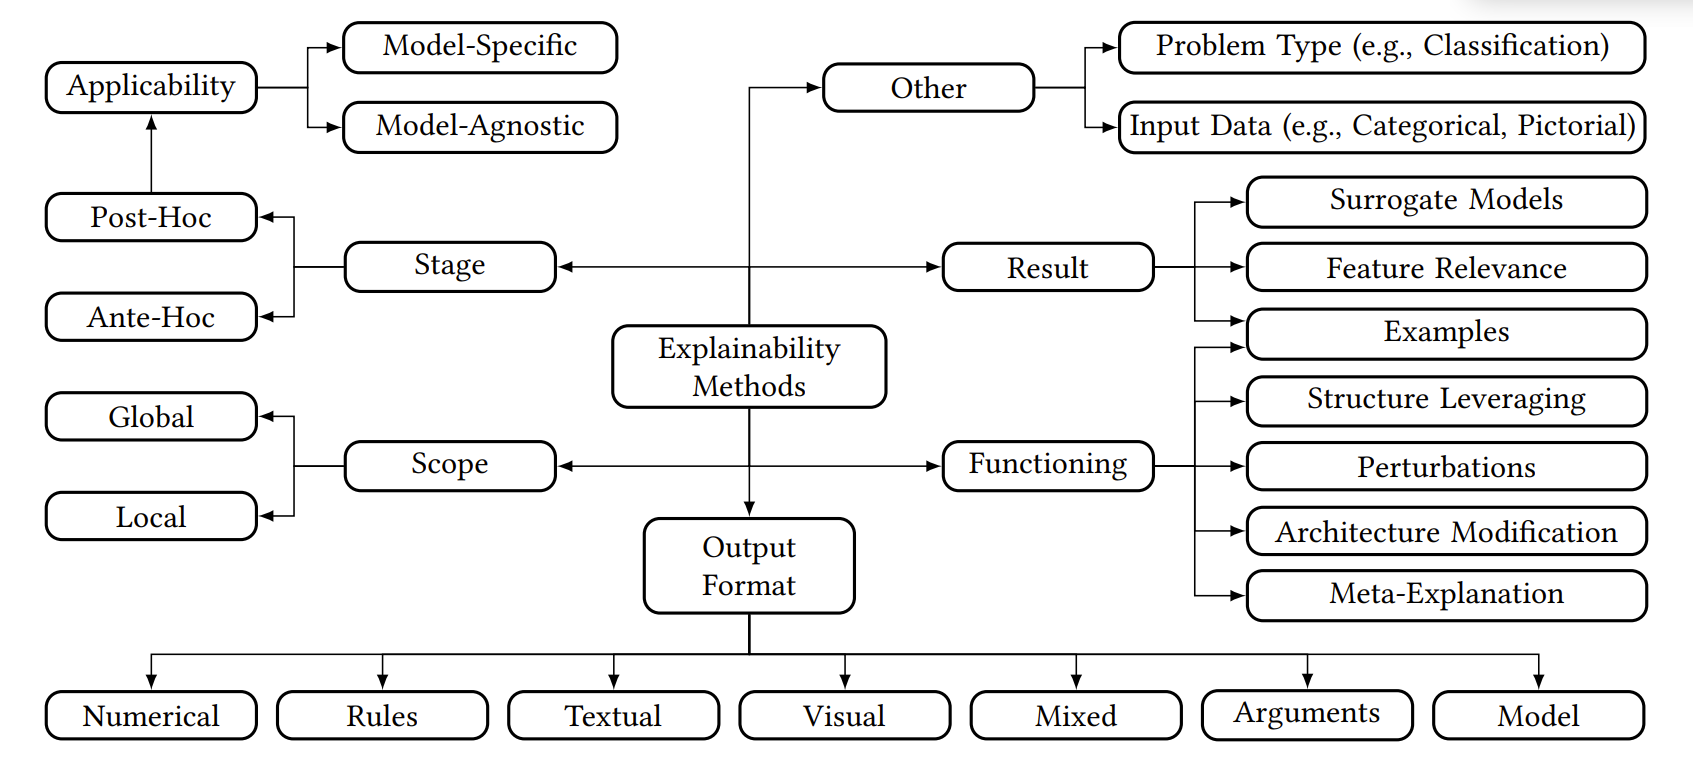
\includegraphics[width=.8\textwidth]{taxonomy_speith}
    \caption{\footnotesize Timo Speith, ``A Review of Taxonomies of Explainable
      Artificial Intelligence (XAI) Methods''. In 2022 ACM Conference on
      Fairness, Accountability, and Transparency (FAccT '22), 2022}
  \end{figure}
\end{frame}

\begin{frame}
  \frametitle{Interpretable models (ante-hoc)}
  \begin{onlyenv}<1>
    \begin{itemize}
    \item Some models afford explanations
    \item Examples, (generalized) linear models, decision trees, $k$-NN
    \item Example: Linear regression
      \begin{equation*}
        \hat{y} = w_1x_1 + \dotsc + w_px_p + b
      \end{equation*}
    \end{itemize}
  \end{onlyenv}
  \begin{onlyenv}<2>
    \begin{itemize}
    \item Result in the bike sharing dataset (model weights)
      \begin{equation*}
        \hat{y} = w_1x_1 + \dotsc + w_px_p + b
      \end{equation*}
    \end{itemize}
    \begin{center}
      \begin{figure}
        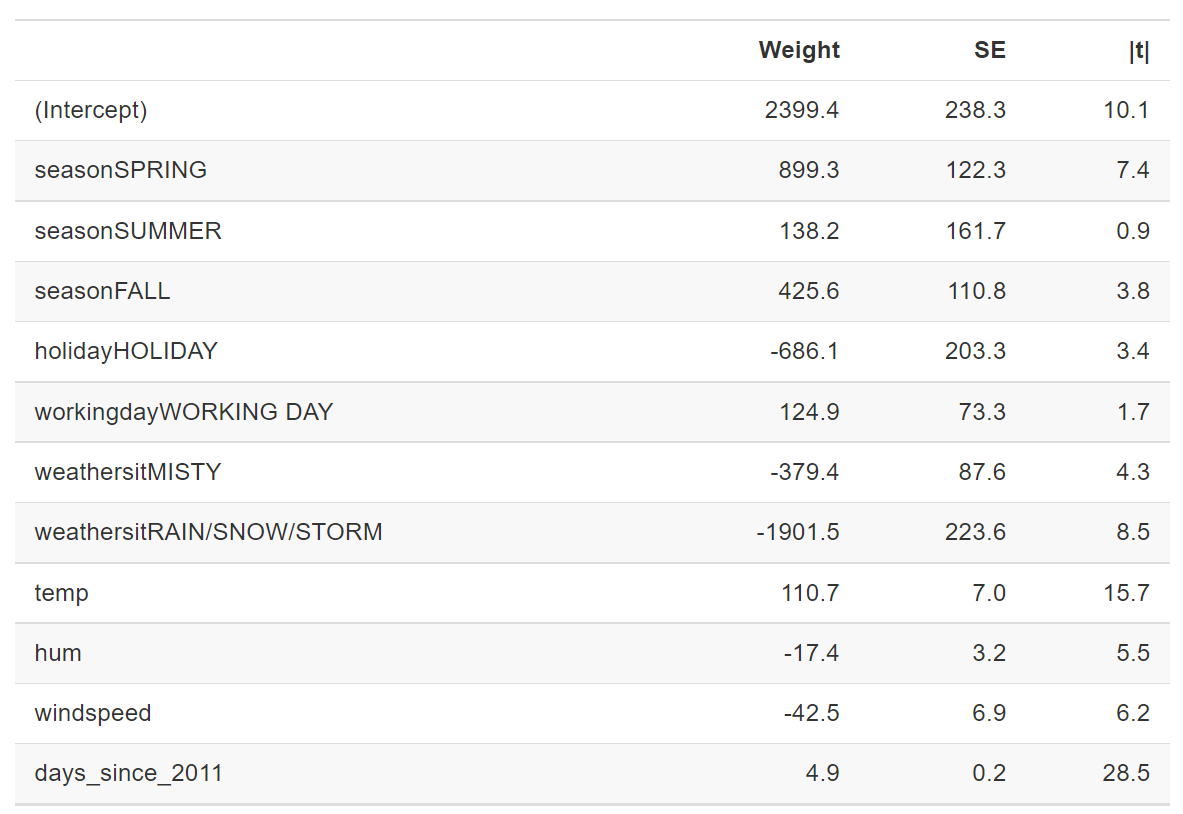
\includegraphics[width=.6\textwidth]{lr_weights}
        \caption{\footnotesize C. Molnar, IML book}
      \end{figure}
    \end{center}
  \end{onlyenv}
  \begin{onlyenv}<3>
    \begin{itemize}
    \item Feature effects (visualization)
      \begin{equation}
        effect_j^{(i)} = w_jx_j^{(i)}
      \end{equation}
    \end{itemize}
    \begin{center}
      \begin{figure}
        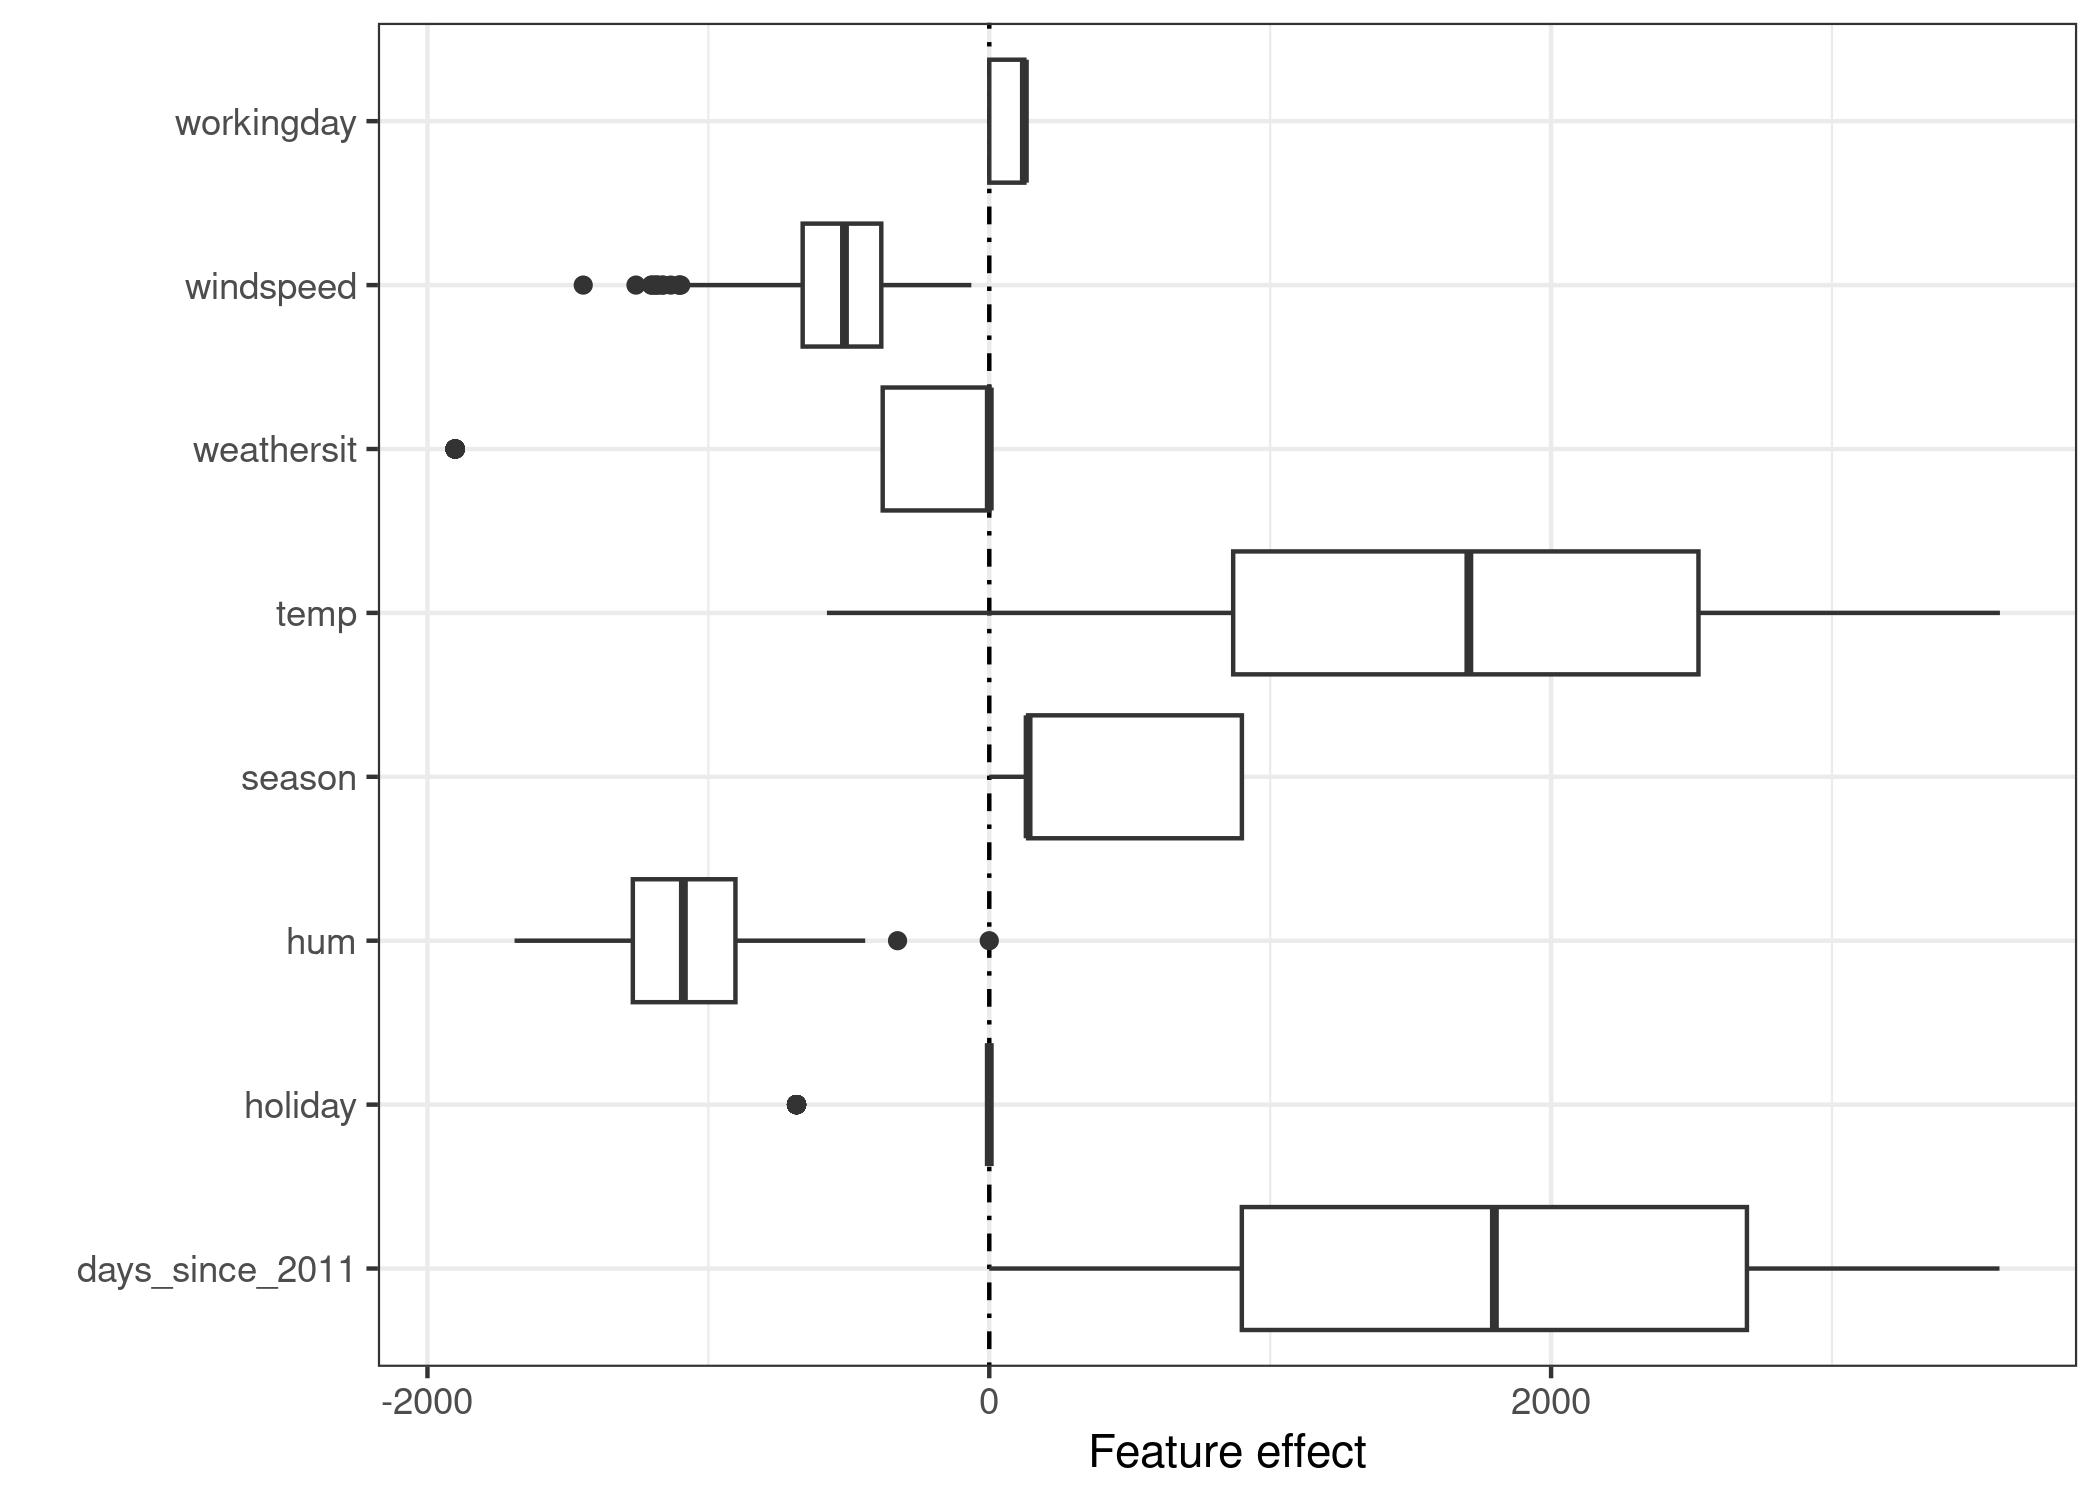
\includegraphics[width=.5\textwidth]{lr_effects}
        \caption{\footnotesize C. Molnar, IML book}
      \end{figure}
    \end{center}
  \end{onlyenv}
\end{frame}

\section{Local, model-agnostic methods}

\begin{frame}
  \frametitle{Local, model agnostic methods}
  \begin{figure}
    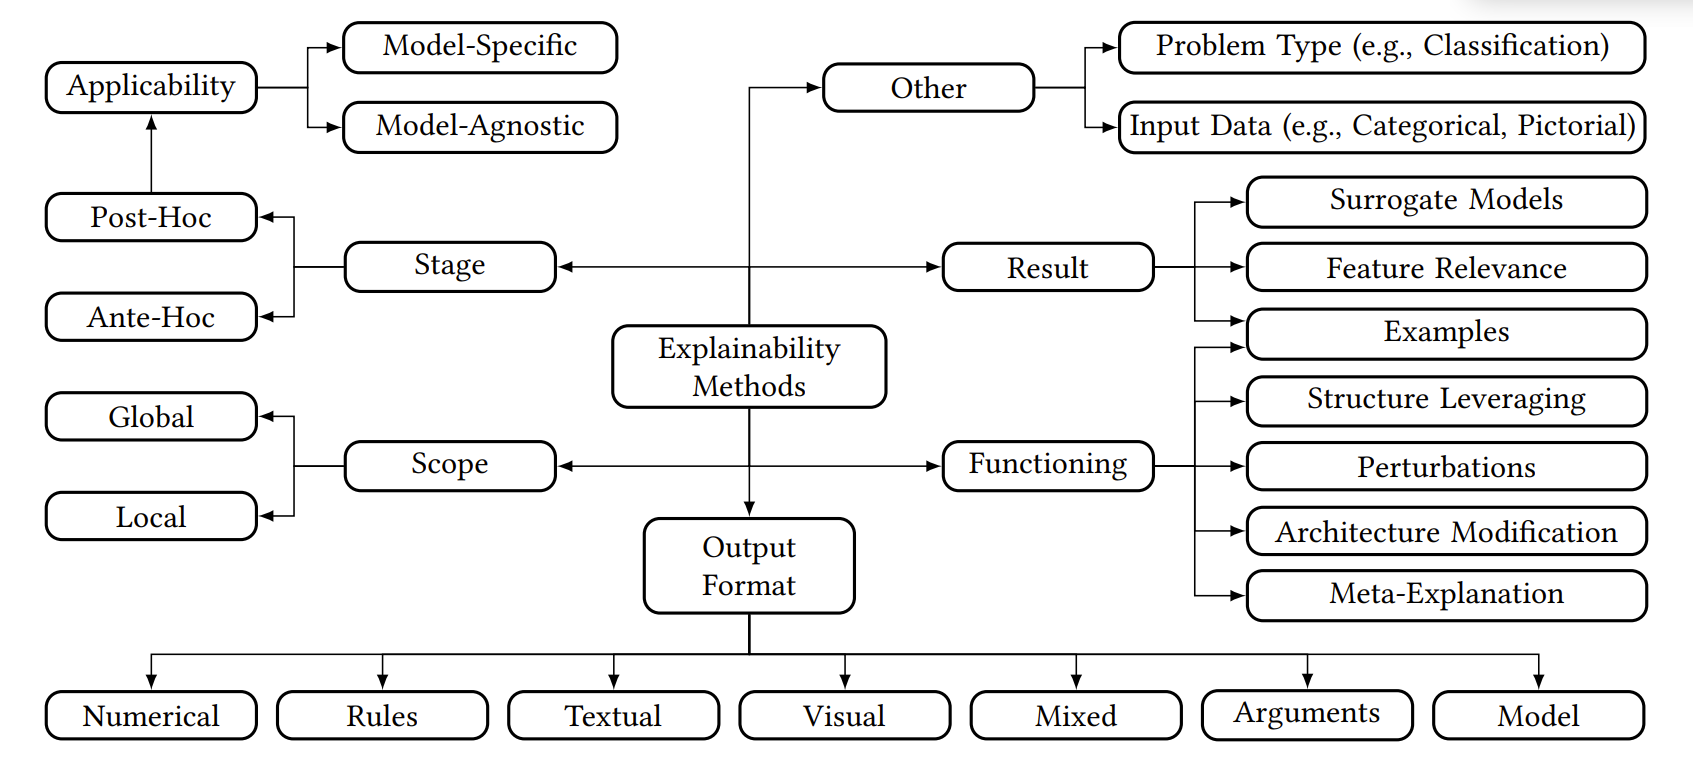
\includegraphics[width=.8\textwidth]{taxonomy_speith}
    \caption{\footnotesize Timo Speith, ``A Review of Taxonomies of Explainable
      Artificial Intelligence (XAI) Methods''. In 2022 ACM Conference on
      Fairness, Accountability, and Transparency (FAccT '22), 2022}
  \end{figure}
\end{frame}

\begin{frame}
  \frametitle{Goal}
  \begin{itemize}
  \item Most models do not afford explanations 
    \begin{itemize}
    \item \orange{we cannot explain them by looking at their parameters}
    \item \orange{we handle these as ``black boxes''}
    \end{itemize}
  \item In this case we apply general interpretability methods
  \item \obf{Local}: Interpret the model's output for a particular input instance
  \item \obf{Global}: Provide a general interpretation of the model's behavior
  \end{itemize}
\end{frame}

\begin{frame}
  \frametitle{LIME - Local Interpretable Model-agnostic
    Explanations\footnote{Ribeiro, Marco Tulio, Sameer Singh, and Carlos
    Guestrin. ``Why should I trust you?: Explaining the predictions of any
    classifier.'' Proceedings of the 22nd ACM SIGKDD international conference
    on knowledge discovery and data mining. ACM (2016)}}
  \begin{onlyenv}<1>
    \begin{itemize}
    \item Idea:
      \begin{itemize}
      \item Train an interpretable model with samples in the neighborhood of the
        target instance, weighted by their proximity
      \end{itemize}
      \begin{equation*}
        \text{explanation(x)} = \arg\min\limits_{g\in G}L(f, g, \pi_x) + \Omega(g)
      \end{equation*}
      \begin{itemize}
      \item $g$ is the interpretable model
      \item $\pi_x$ is the weighting function (e.g., a radial basis function
        kernel)
      \item $\Omega(g)$ is a regularizer for $g$ (e.g., LASSO, or limit on the
        number of features)
      \end{itemize}
    \end{itemize}
  \end{onlyenv}
  \begin{onlyenv}<2>
    \begin{itemize}
    \item Idea (visualization)
    \end{itemize}
    \begin{figure}
      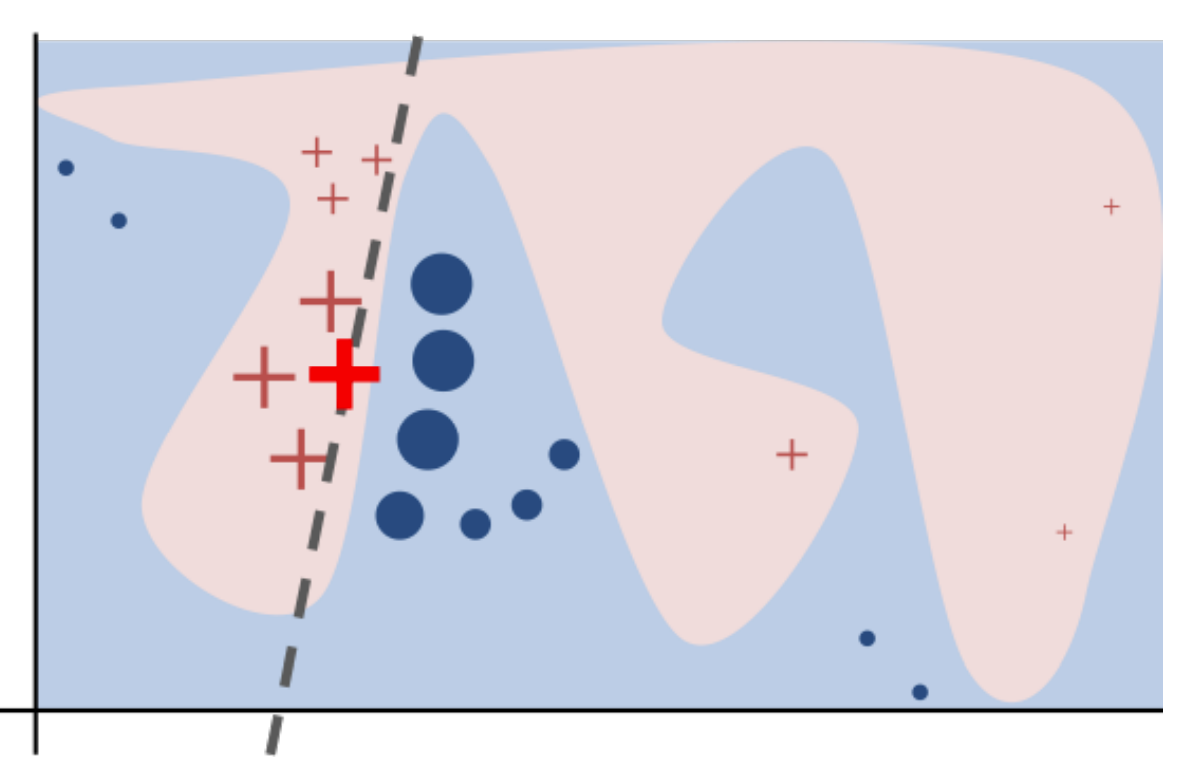
\includegraphics[width=.4\textwidth]{lime_idea}
      \caption{\footnotesize Ribeiro et al, 2016}
    \end{figure}
  \end{onlyenv}
  \begin{onlyenv}<3>
    \begin{itemize}
    \item Application on text data
    \end{itemize}
    \begin{figure}
      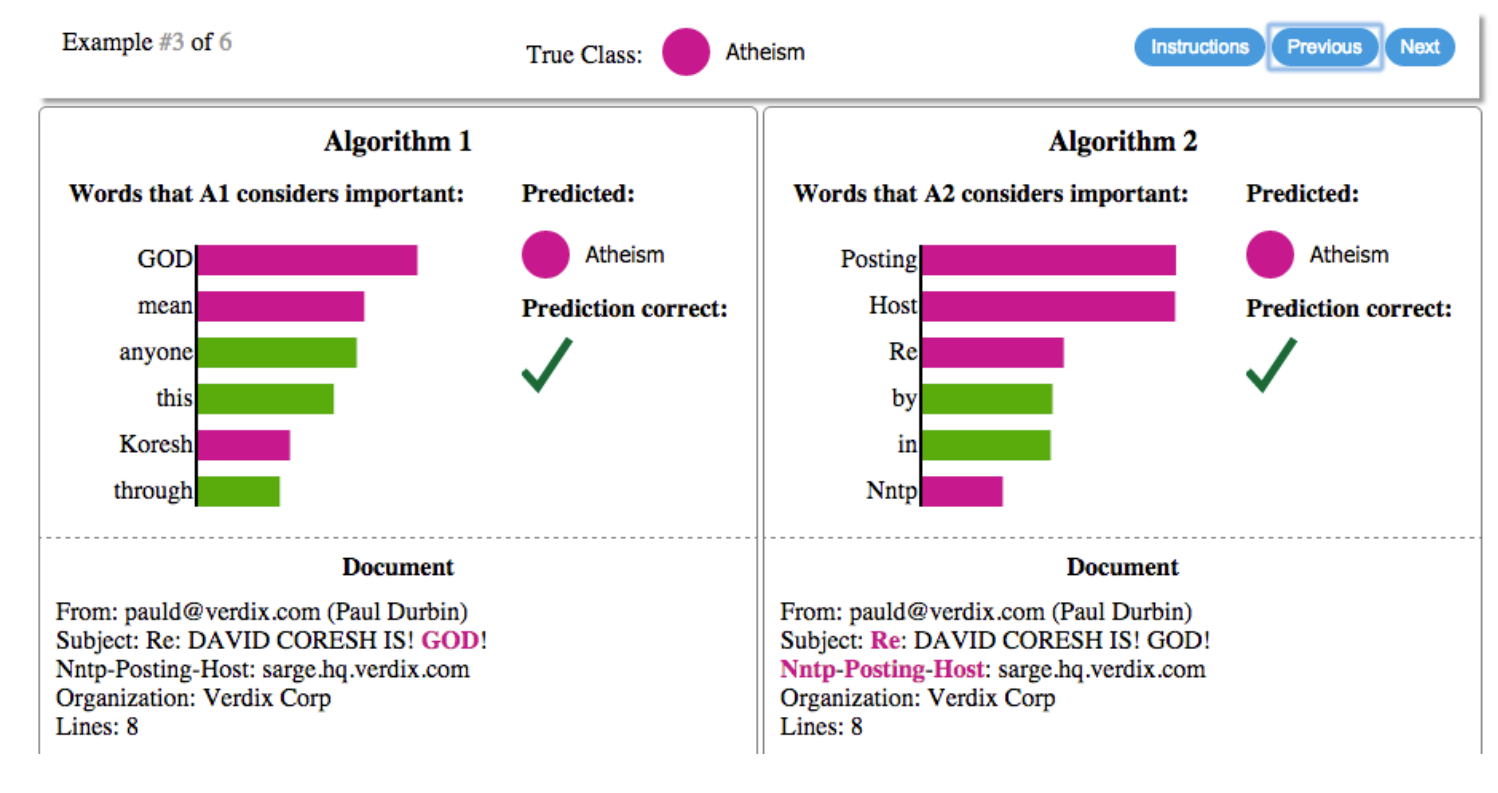
\includegraphics[width=.6\textwidth]{lime_atheism}
      \caption{\footnotesize Ribeiro et al, 2016}
    \end{figure}
  \end{onlyenv}
\end{frame}

\begin{frame}
  \frametitle{LIME with images}
  \begin{itemize}
  \item Instead of features, we use superpixels (e.g., extracted via quick shift)
  \item We obtain samples by ``removing'' superpixels (e.g., by replacing their
    pixels with medium gray)
  \end{itemize}
  \begin{figure}
    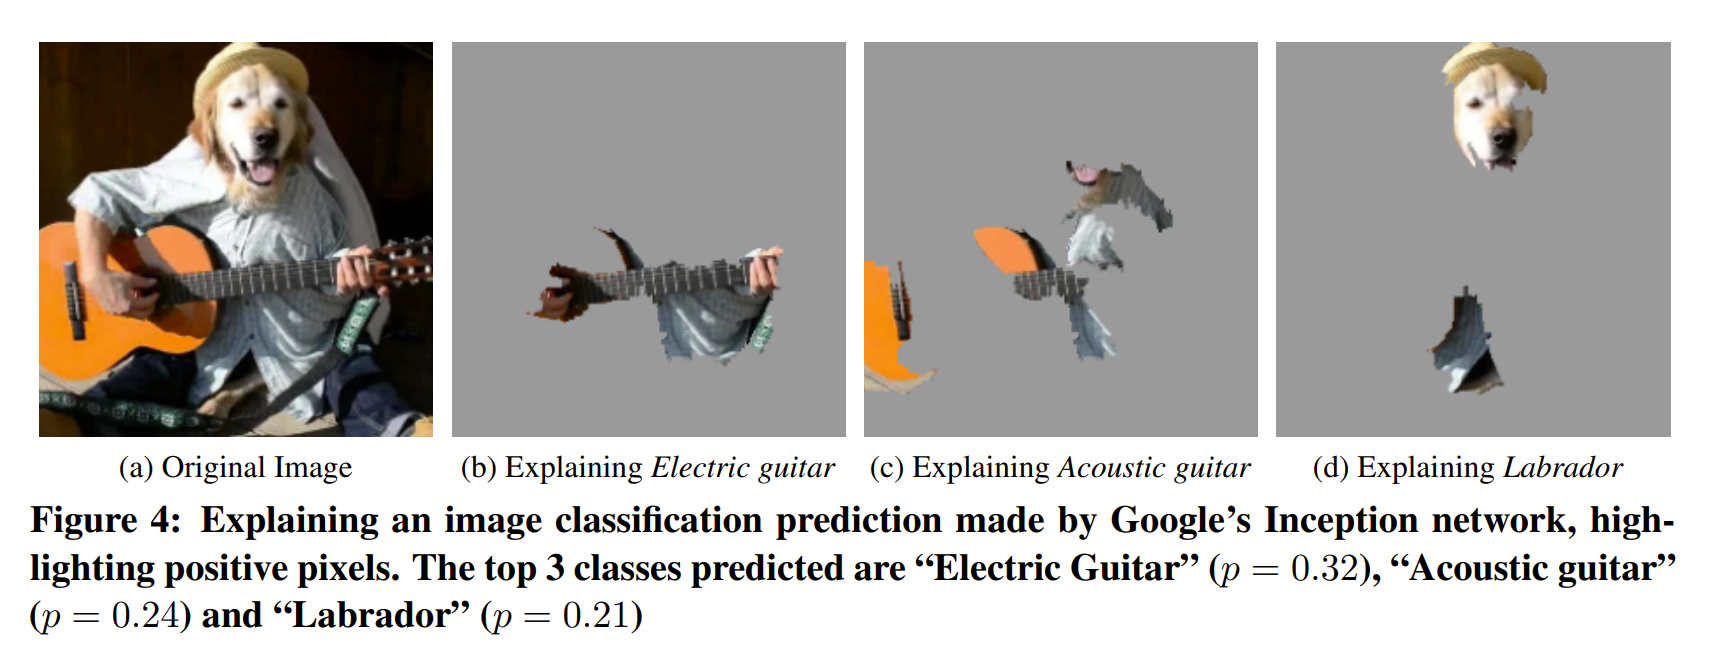
\includegraphics[width=.8\textwidth]{LIME}
    \caption{\footnotesize Ribeiro et al., 2016}
  \end{figure}
\end{frame}

% TODO
\begin{frame}
  \frametitle{SHAP}
  \begin{itemize}
  \item Let $\phi_j$ be the feature attribution of the $j$-th feature
  \item Then,
    \begin{equation*}
      g(z') = \phi_0 + \sum\limits_{j = 1}^{M}\phi_jz_j'
    \end{equation*}
    \begin{itemize}
    \item $z' \in \left\{0, 1\right\}^M$ (all 1's for the target instance)
    \item General definition - applies to LIME too!
    \end{itemize}
  \end{itemize}
  \begin{figure}
    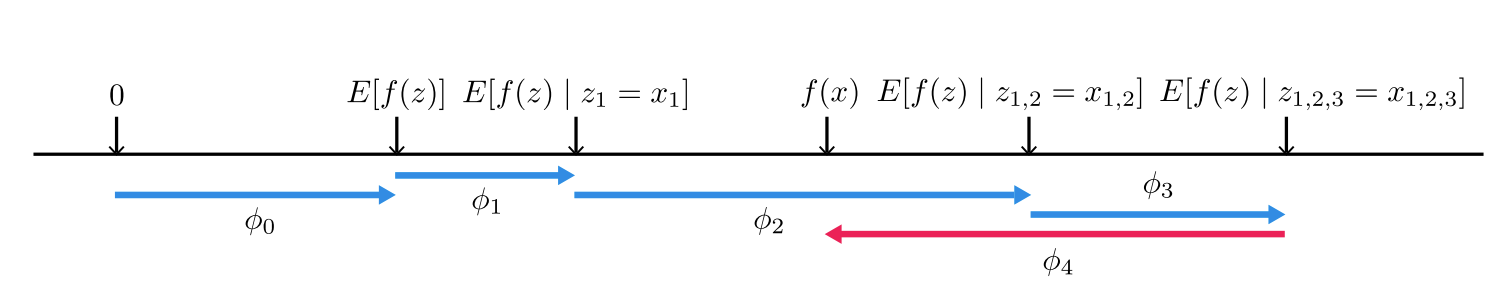
\includegraphics[width=.8\textwidth]{shap_attributions}
    \caption{\footnotesize S.M. Lundberg and S.I Lee. A unified approach to
        interpreting model predictions. Advances in neural information
        processing systems, 2017}
  \end{figure}
\end{frame}

\begin{frame}
  \frametitle{Kernel SHAP - procedure}
  \begin{onlyenv}<1>
  \begin{enumerate}
  \item Sample $K$ binary vectors $z'_k \in \left\{0, 1\right\}^M$
  \item Get a value $x'$ by using mapping function $h_x(z'_k)$
    \begin{itemize}
      \item Get value of $x_j$ if $z'_j = 1$, get the value from another
        randomly selected dataset sample if $z'_j = 0$
    \end{itemize}
  \item Get prediction $\hat{f}(h_x(z'_k))$
  \item Compute weight using SHAP kernel (which has some nice properties - see paper)
  \item Fit linear model
  \item $\phi_k$ are the linear model coefficients
  \end{enumerate}
  \end{onlyenv}
  \begin{onlyenv}<2>
      \begin{figure}
    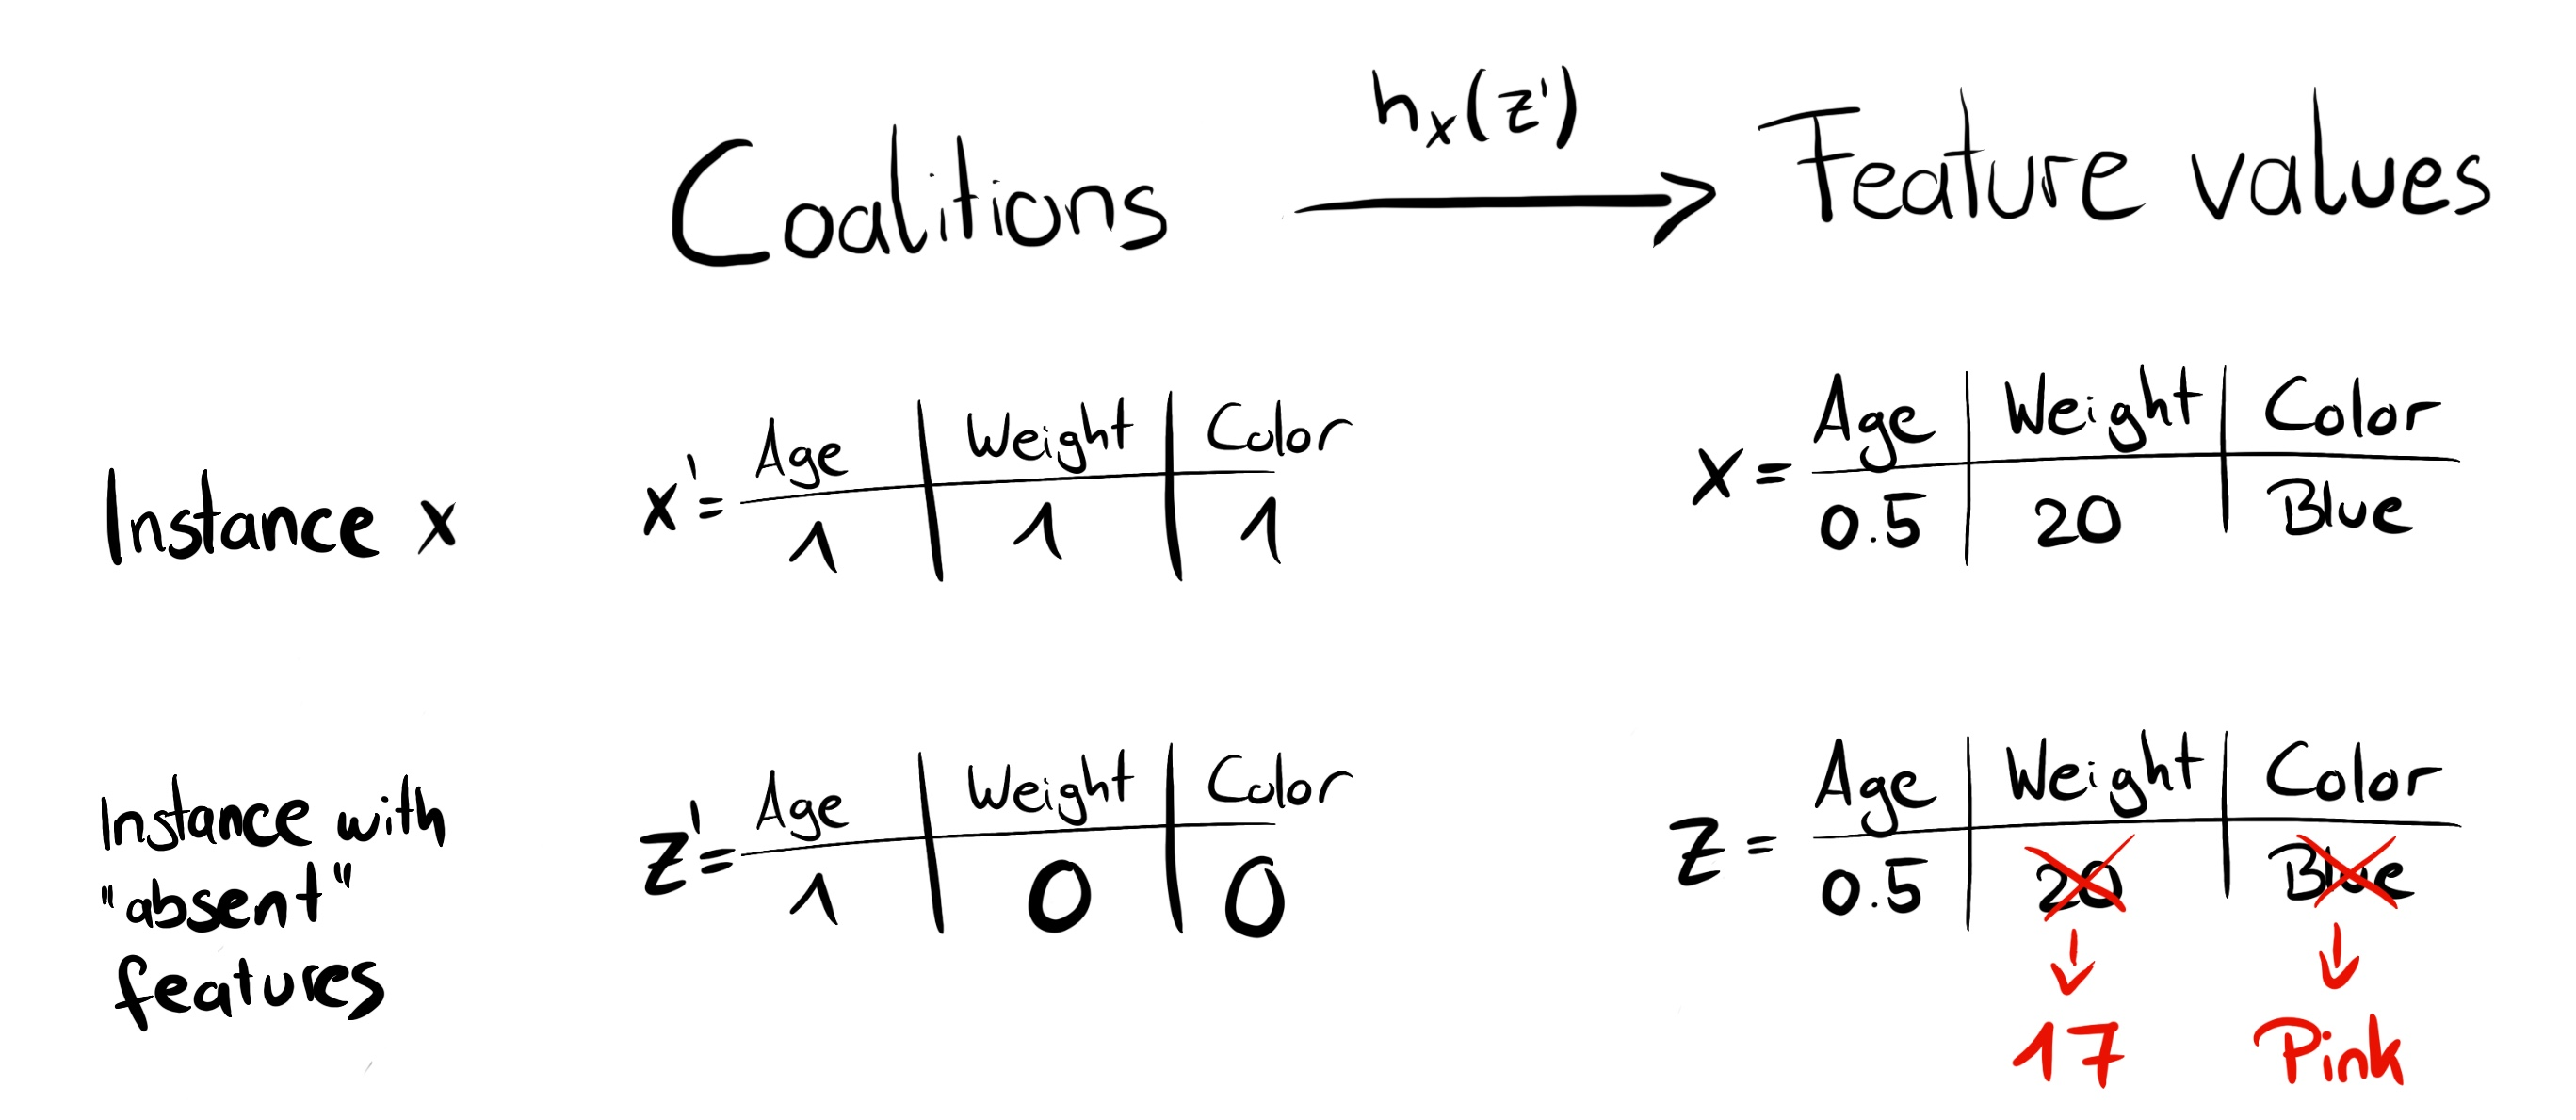
\includegraphics[width=.8\textwidth]{shap_example}
    \caption{\footnotesize C. Molnar, IML book}
  \end{figure}
  \end{onlyenv}
\end{frame}

\begin{frame}
    \frametitle{SHAP for images}
  \begin{itemize}
  \item Similar idea with LIME, apply SHAP on superpixels
    \begin{figure}
      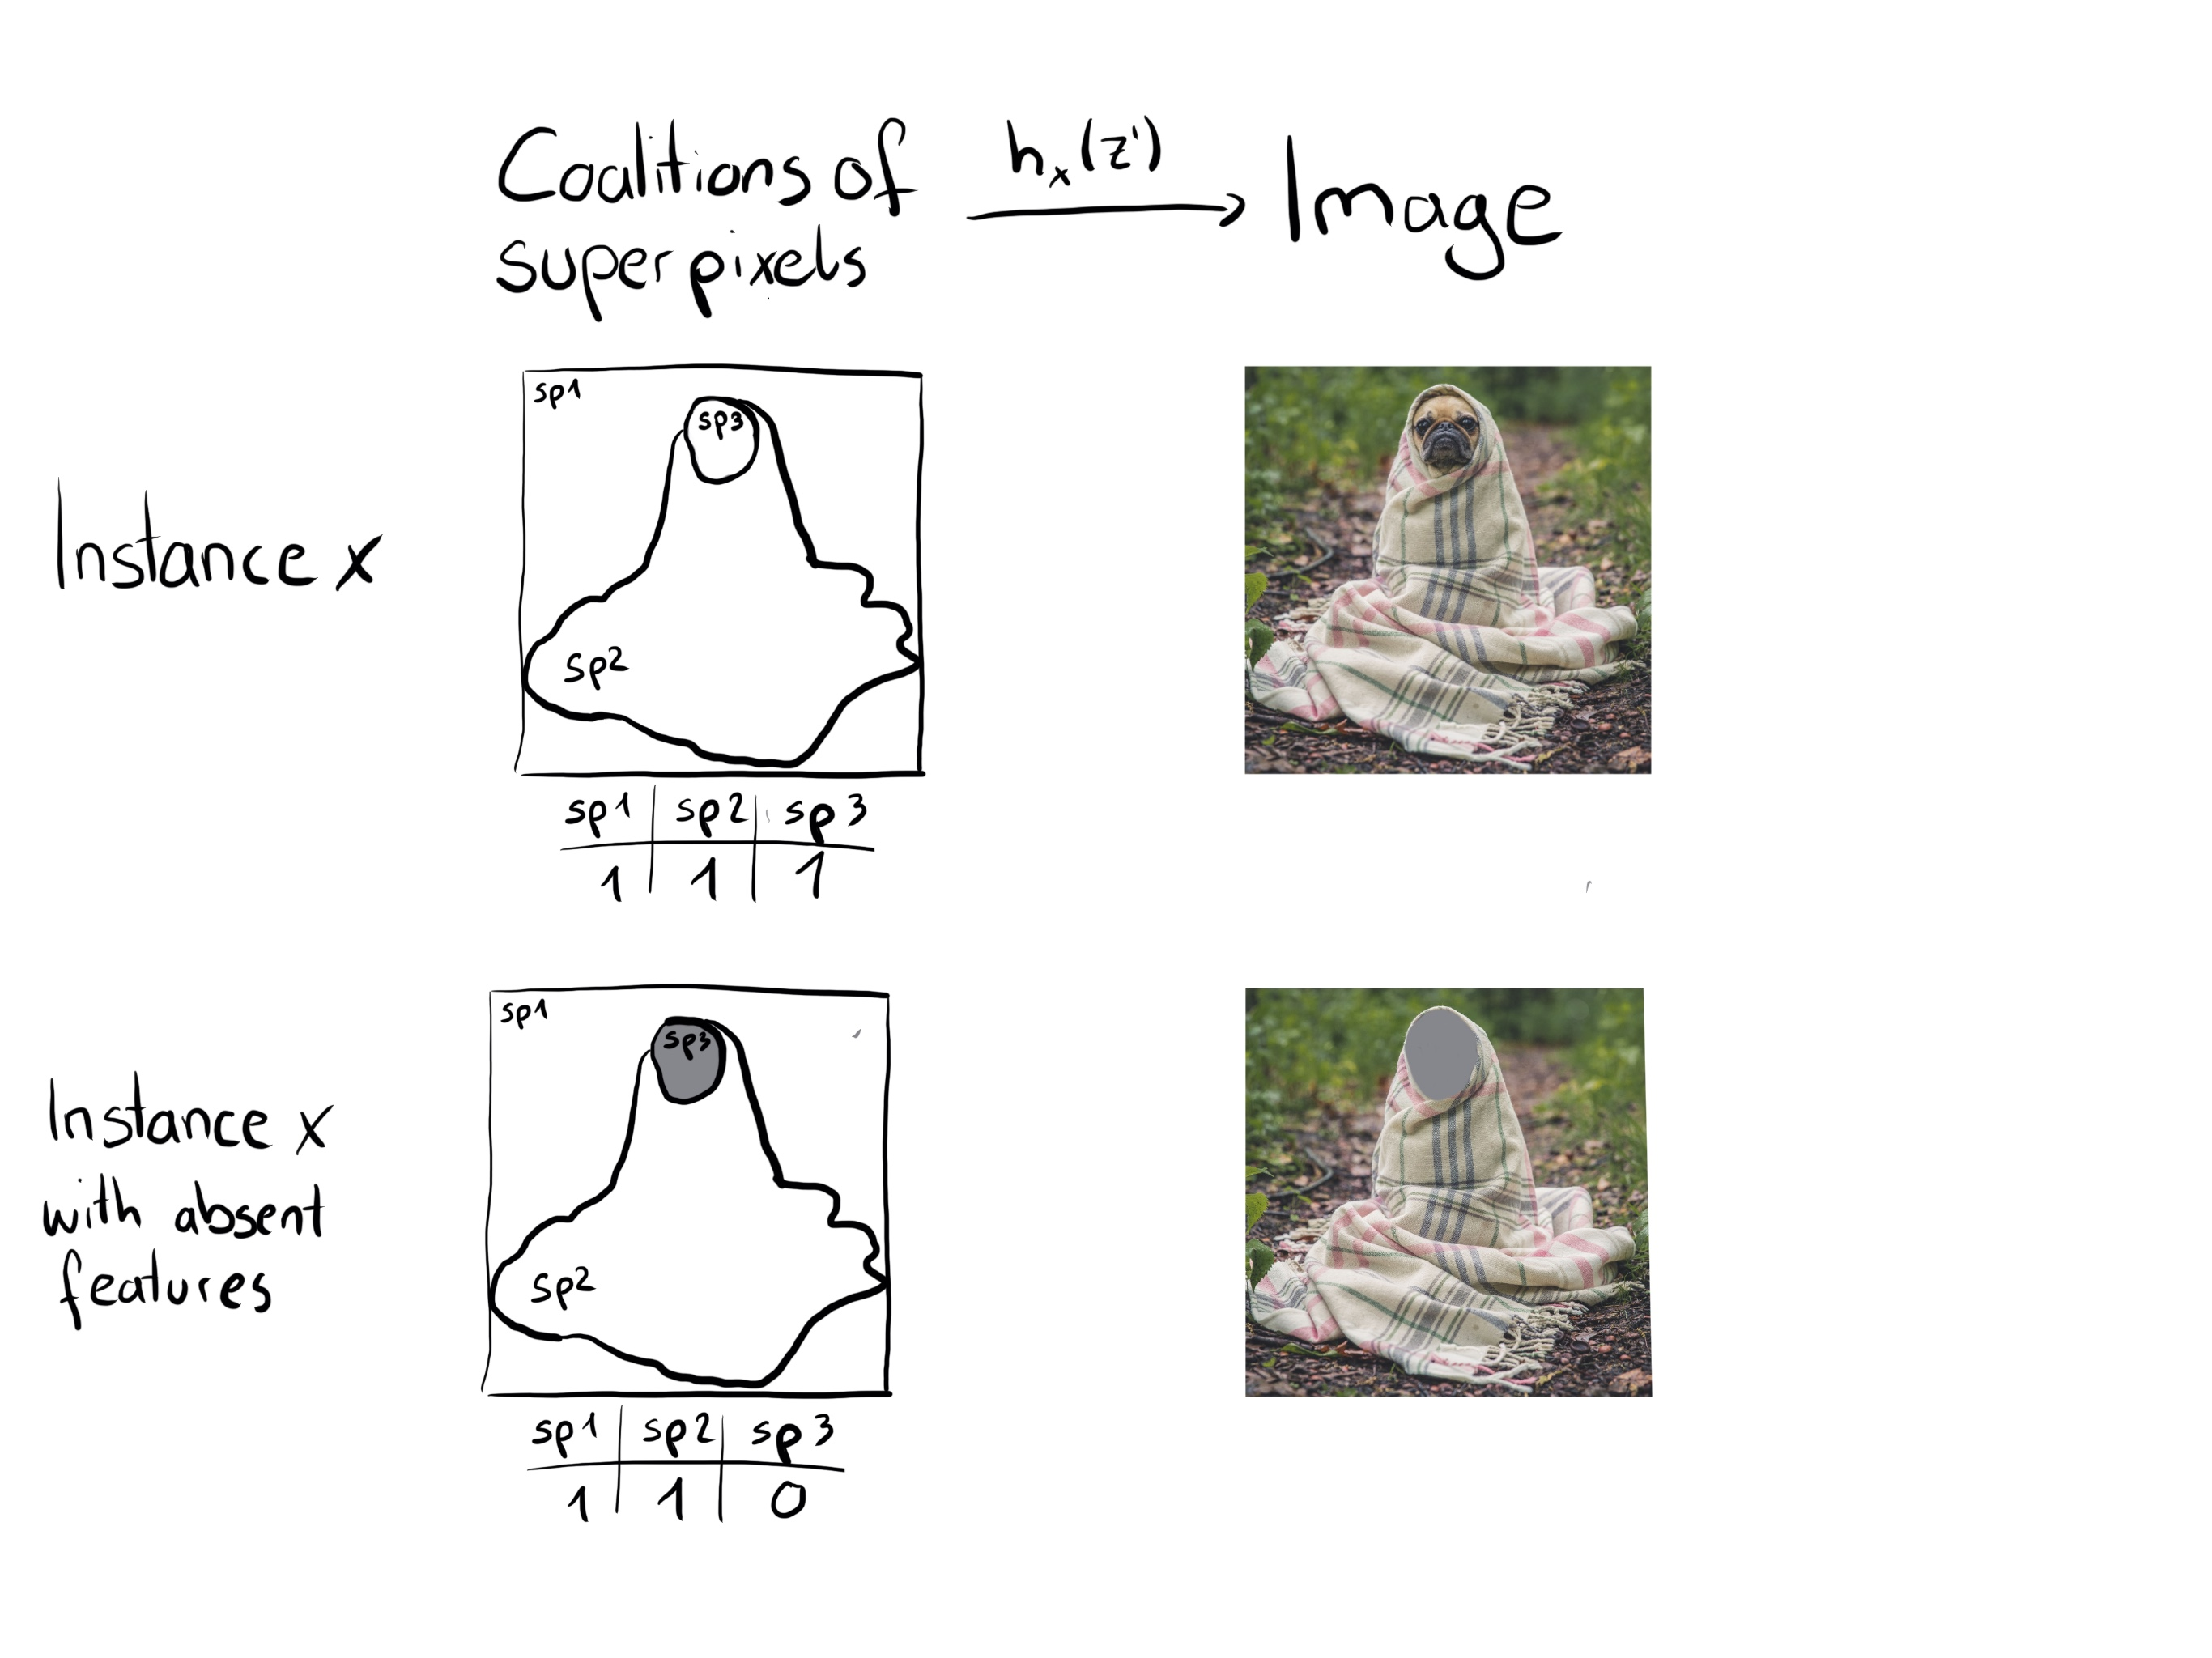
\includegraphics[width=.6\textwidth]{shap-superpixel}
      \caption{\footnotesize C. Molnar, IML book}
    \end{figure}
  \end{itemize}
\end{frame}

\section{Methods for CNN interpretation}

\begin{frame}
  \frametitle{Visualization of extracted features}
  \begin{figure}
    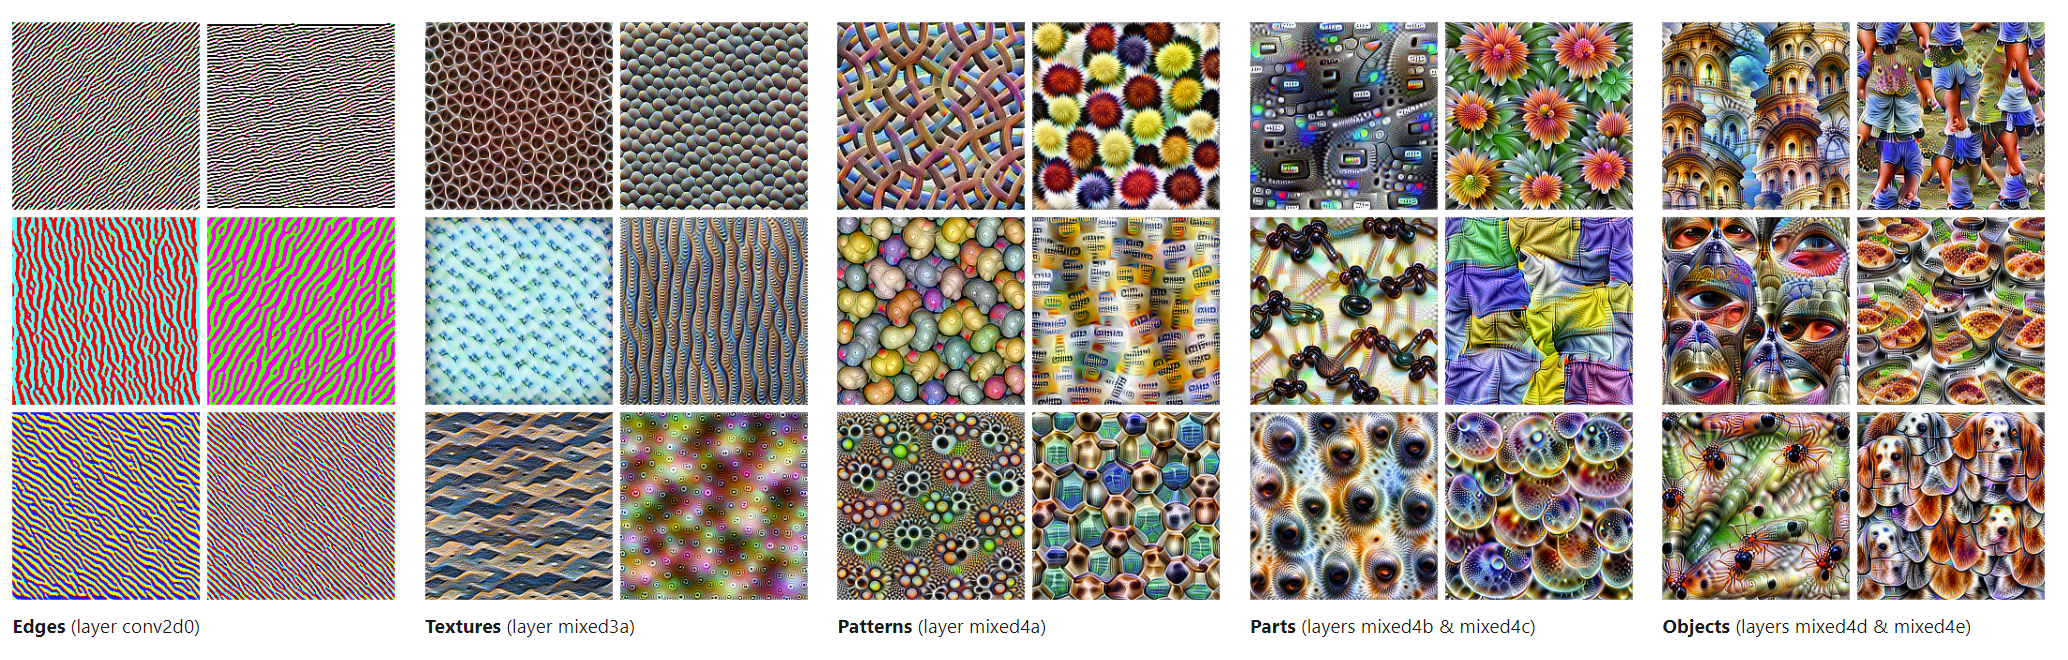
\includegraphics[width=\textwidth]{features}
    \caption{\footnotesize \url{https://distill.pub/2017/feature-visualization/}}
  \end{figure}
  \begin{itemize}
  \item These images maximize the activation of specific filters of an
    Inception-V1 network at different depths
  \end{itemize}
\end{frame}

\begin{frame}
  \frametitle{Pixel attribution / Saliency maps}
  Methods that visualize the contribution of different areas of an image in the
  final decision
  \begin{itemize}
  \item Occlusion- or perturbation-based methods)
    \begin{itemize}
    \item SHAP / LIME belong in this category
    \end{itemize}
  \item Gradient-based methods
  \end{itemize}
\end{frame}

\begin{frame}
  \frametitle{Saliency maps (vanilla gradient)}
  \begin{enumerate}
  \item Forward pass of the input image, $I_0$
  \item Compute the derivative of the output/class of interest $S_c$, with
    respect to the input
    \begin{equation*}
      E_{grad}(I_0) = \frac{\partial S_c}{\partial I}\Bigr|_{I=I_0}
    \end{equation*}
  \item visualize the resulting image
  \end{enumerate}
  Question: How to handle $ReLU$;
  \begin{align*}
    X_{n+1} &= \max(0, X_n)\\
    \frac{\partial f}{\partial X_n} &= \frac{\partial f}{\partial X_{n+1}}\mathbf{I}(X_n > 0)
  \end{align*}
\end{frame}

\begin{frame}
  \frametitle{Saturation}
  \begin{figure}
    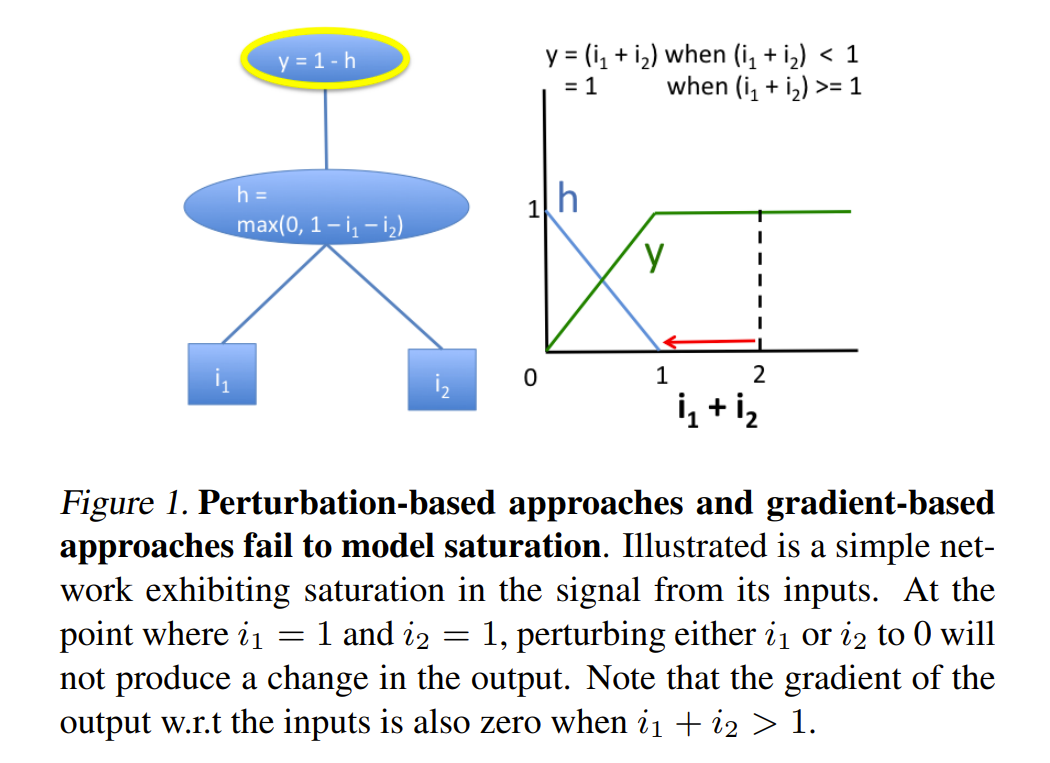
\includegraphics[width=.6\textwidth]{saturation}
    \caption{\footnotesize A. Shrikumar, P. Greenside, and A.
      Kundaje. ``Learning important features through propagating activation
      differences.'' Proceedings of the 34th International Conference on
      Machine Learning-Volume 70. JMLR. org, (2017).}
  \end{figure}
  \begin{itemize}
  \item Variations of Saliency Maps: DeconvNets, Guided Backpropagation
    \begin{itemize}
    \item Different handling of $ReLU$, do not completely overcome the
      saturation problem
    \end{itemize}
  \end{itemize}
\end{frame}

\begin{frame}
  \frametitle{GradCAM}
  Different approach; starting from the output of the next to last layer
  (before softmax) for class $c$, and for activations of features $A^{k}$ of a layer $A$
  (often the last conv layer)
  \begin{enumerate}
  \item Apply global average pooling on derivatives
    \begin{equation*}
      a_{k}^{c} = \frac{1}{Z}\sum\limits_i\sum\limits_j\frac{\partial
        y^{c}}{\partial A^{k}_{i, j}}
    \end{equation*}
    \begin{itemize}
    \item Coefficients $a_{k}^{c}$ quantify the importance of layer $k$ for
      detecting class $c$
    \end{itemize}
  \item Use weighted sum of activations to produce the final visualization
    \begin{equation*}
      L_{GradCAM}^{c} = ReLU\left(\sum\limits_ka_kA^{k}\right)
    \end{equation*}
  \end{enumerate}
\end{frame}

\begin{frame}
  \frametitle{Example - initial images}
  \begin{figure}
    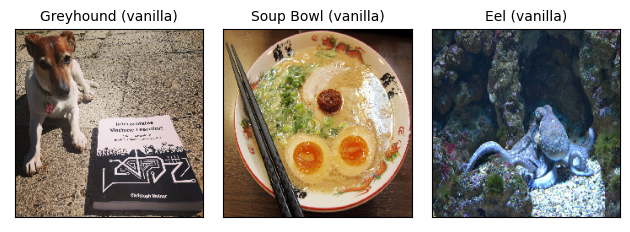
\includegraphics[width=.6\textwidth]{original-images}
    \caption{\footnotesize C. Molnar, IML book}
  \end{figure}

\end{frame}

\begin{frame}
  \frametitle{Example - gradient-based interpretations}
  \begin{figure}
    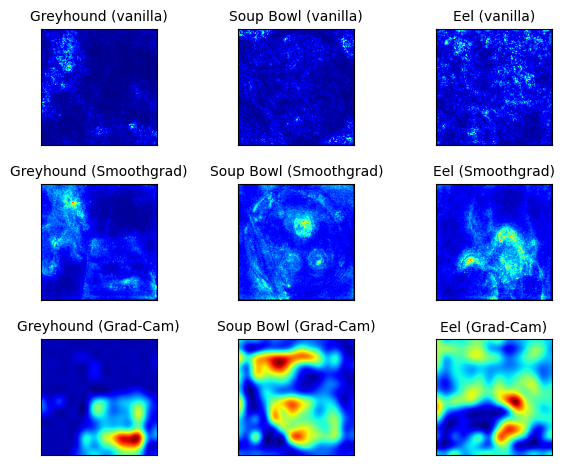
\includegraphics[width=.6\textwidth]{grad}
    \caption{\footnotesize C. Molnar, IML book}
  \end{figure}
\end{frame}

\begin{frame}
  \frametitle{Problems - drawbacks (1)}
  \begin{itemize}
  \item Evaluation of these methods is commonly qualitative - we don't know if
    the interpretation is correct
  \item It has been demonstrated that these methods are very sensitive
    \footnote{A. Ghorbani, A. Abid, and J. Zou. ``Interpretation of
    neural networks is fragile.'' Proceedings of the AAAI Conference on
    Artificial Intelligence. Vol. 33. 2019.}
    \begin{itemize}
    \item \orange{Very small changes of the input can lead to the same output but
      completely different interpretation}
    \end{itemize}
  \end{itemize}
\end{frame}

\begin{frame}
  \frametitle{Problems - drawbacks (2)}
  \begin{itemize}
  \item It has also been shown that some of these methods are unreliable\footnote{P-J Kindermans, S. Hooker, J. Adebayo, M. Alber,
    K. T. Sch\"{u}tt,  S. D\"{a}hne, D. Erhan and B. Kim. ``The (un)
    reliability of saliency methods.'' In Explainable AI: Interpreting,
    Explaining and Visualizing Deep Learning, pp. 267-280. Springer, Cham
    (2019)}
    \begin{itemize}
    \item \orange{Adding constant pixel offset and changing the bias term of
      the first layer leads to the same predictions and derivatives, but to
      different interpretations}
    \end{itemize}
  \item It has finally been show that often these methods do not depend on the
    model or the data (and are therefore not useful for interpretation), similarly to an edge
    detector\footnote{J. Adebayo, J. Gilmer, M. Muelly, I. Goodfellow, M. Hardt
    and B. Kim. ``Sanity checks for saliency maps.'' arXiv preprint
    arXiv:1810.03292 (2018)}
  \end{itemize}
\end{frame}


\begin{frame}
  \frametitle{Example - similarity to edge detectors}
  \begin{figure}
    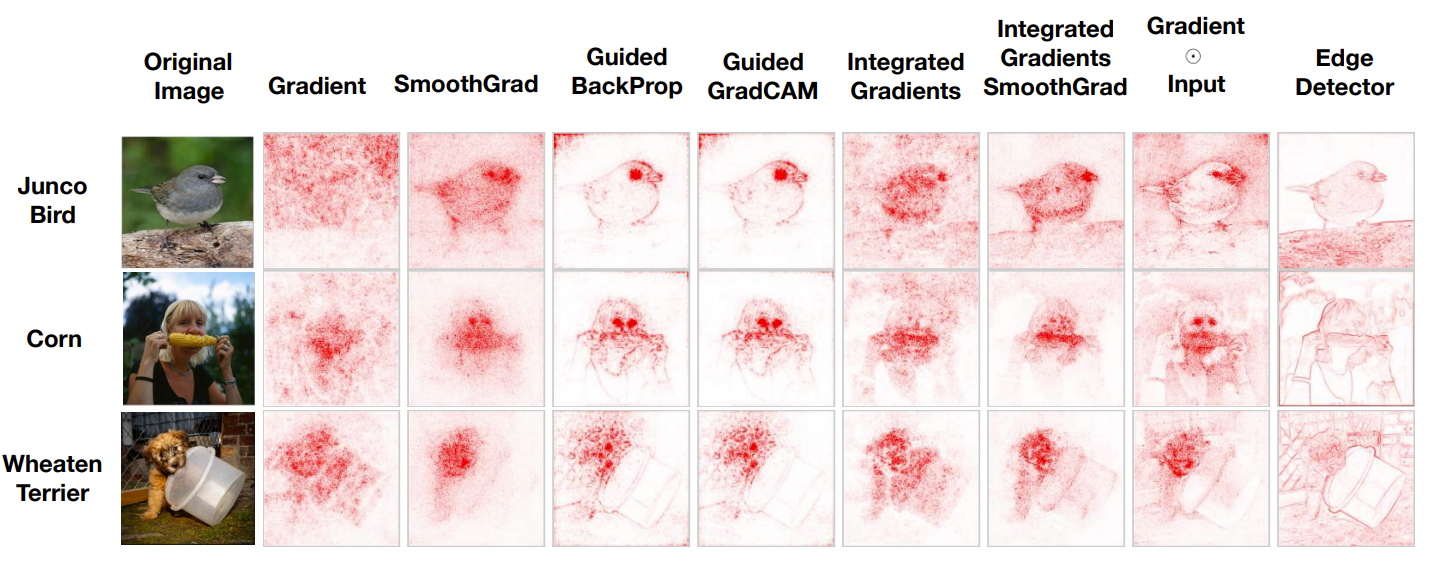
\includegraphics[width=.8\textwidth]{edge_detectors}
    \caption{\footnotesize Adebayo et al, 2018}
  \end{figure}
\end{frame}

\begin{frame}
  \frametitle{Example - randomization test}
  \begin{figure}
    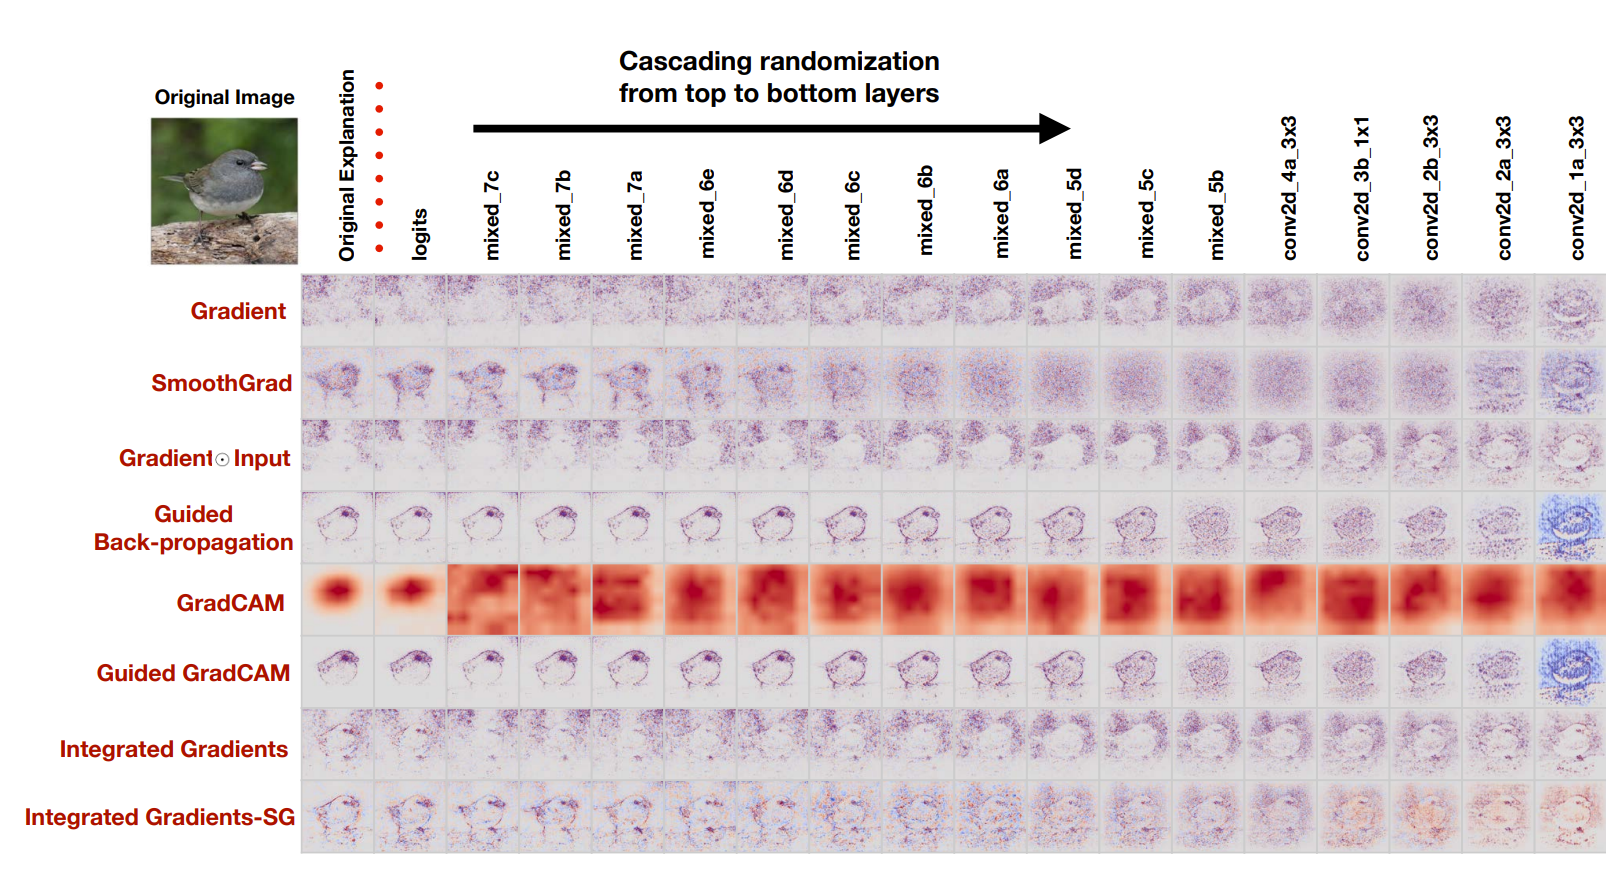
\includegraphics[width=.8\textwidth]{randomization_test}
    \caption{\footnotesize Adebayo et al, 2018}
  \end{figure}
\end{frame}

\section{Global, model agnostic methods}

\begin{frame}
  \frametitle{Goal}
  \begin{itemize}
  \item Our aim is to produce interpretations that describe the model's
    behavior as a whole 
  \item We focus on tabular data, and the result is usually a plot
  \end{itemize}
  \begin{figure}
    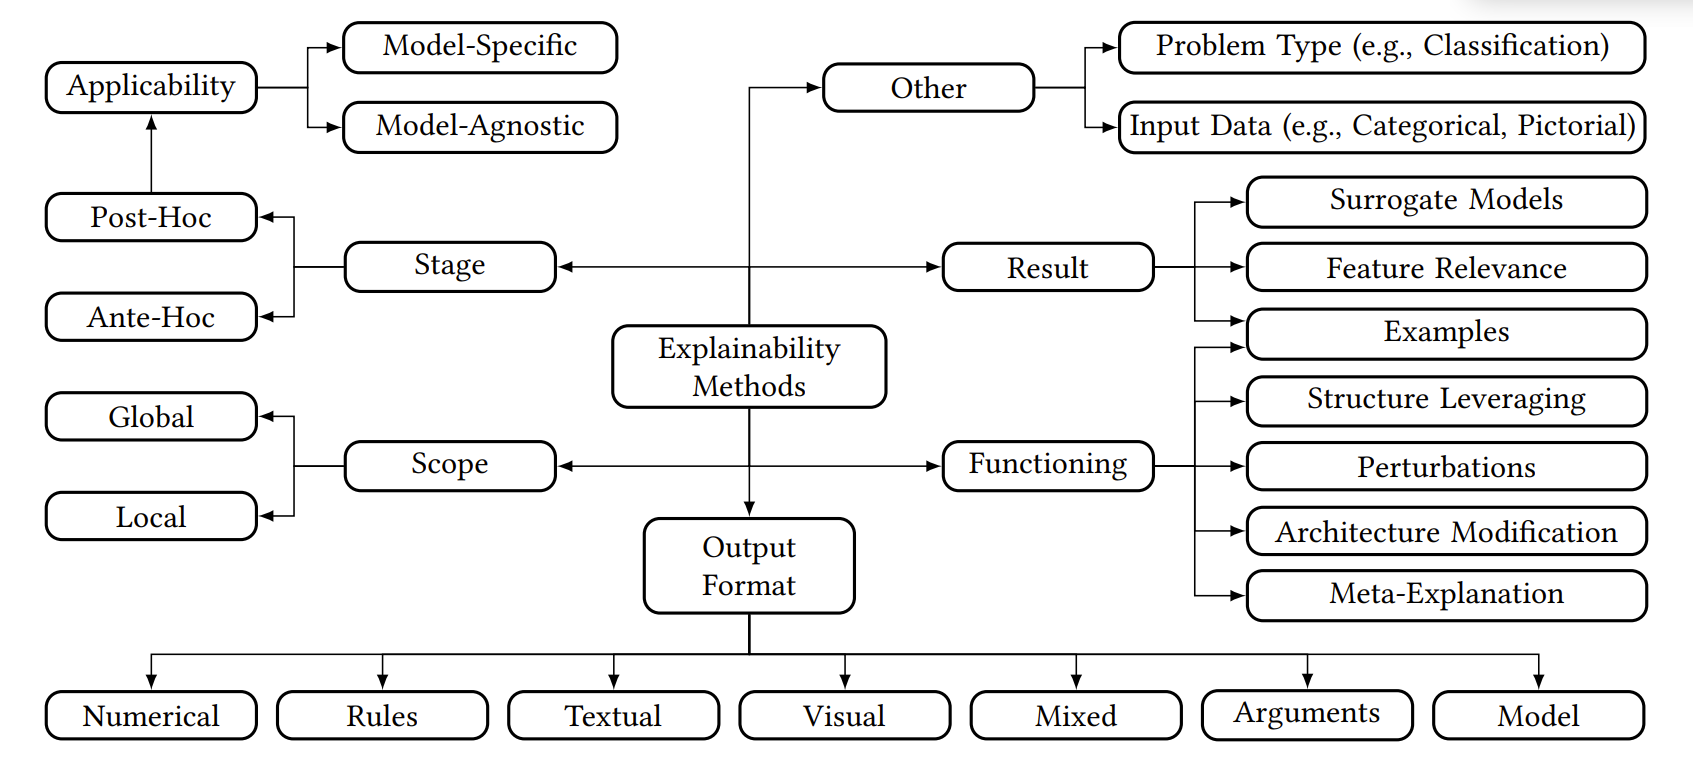
\includegraphics[width=.6\textwidth]{taxonomy_speith}
  \end{figure}
\end{frame}

\begin{frame}
  \frametitle{Feature effect methods}
  \begin{itemize}
  \item \(x_s \rightarrow \) feature of interest, \(\Vx_c \rightarrow\) other features
  \item How do we isolate the effect of \(x_s\)?
    %% \item Προβλήματα:
    %%   \begin{itemize}
    %%   \item Συσχετισμένα χαρ/κά
    %%   \item Η \(f\) έχει μάθει σύνθετες αλληλεπιδράσεις 
    %%   \end{itemize}
  \end{itemize}
\end{frame}

\begin{frame}
  \frametitle{Partial Dependence Plots (PDP)}
  \begin{onlyenv}<1>
    \begin{itemize}
    \item Proposed by J. Friedman on 2001\footnote{J. Friedman. ``Greedy
    function approximation: A gradient boosting machine.'' Annals of statistics
    (2001): 1189-1232} and is the marginal \obf{effect} of a feature to the
      model output:
      \begin{equation*}
        \hat{f_s(x_s)} = E_{X_c}\left[\hat{f}(x_s, X_c)\right] =
        \int\hat{f}(x_s, X_c)d\mathbb{P}(X_c)
      \end{equation*}
      where $x_s$ is the feature whose effect we wish to compute and $X_c$ is a
      random variable corresponding to the rest of the model's features
    \item Computation:
      \begin{equation*}
        \hat{f}_s(x_s) = \frac{1}{n}\sum\limits_{i=1}^{n}\hat{f}(x_s, \Vx_c^{(i)})
      \end{equation*}
    \end{itemize}
  \end{onlyenv}
  \begin{onlyenv}<2>
    \obf{Example 1 (continuous):}
    \begin{figure}
      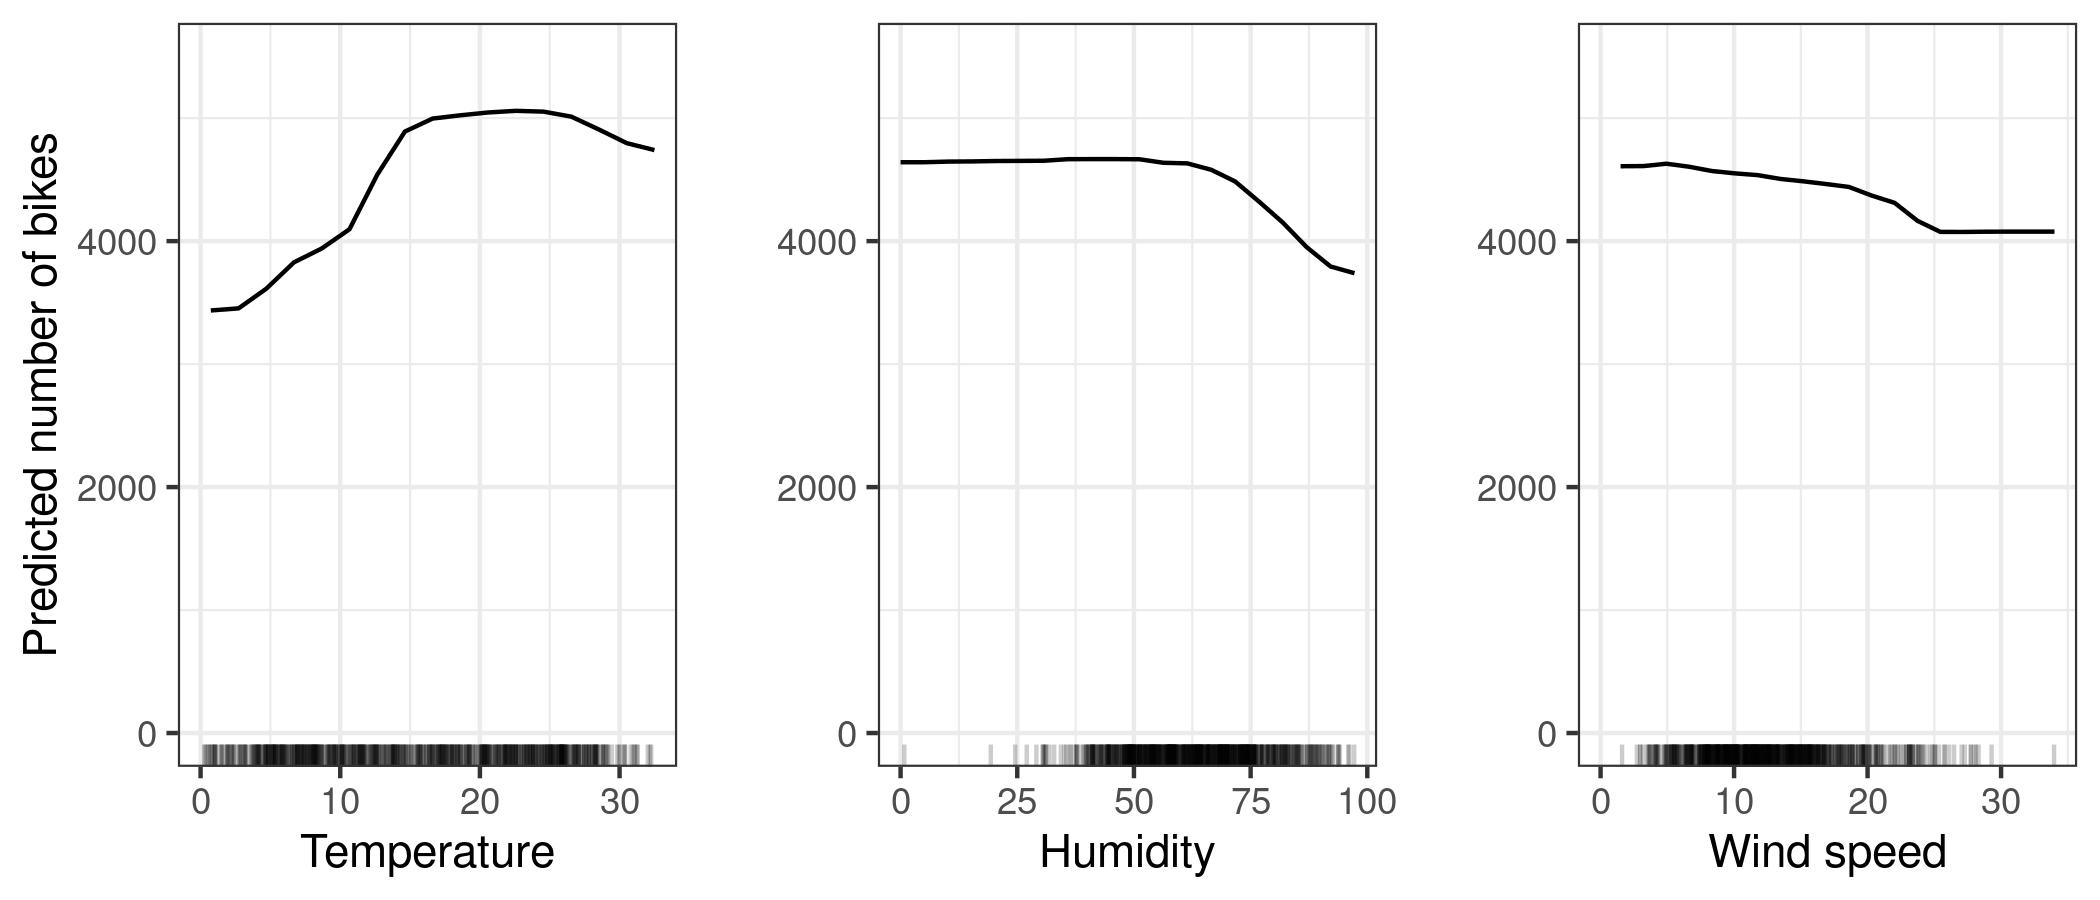
\includegraphics[width=.6\textwidth]{pdp-bike-1}
      \caption{\footnotesize C. Molnar, IML book}
    \end{figure}
  \end{onlyenv}
  \begin{onlyenv}<3>
    \obf{Example 2 (categorical):}
    \begin{figure}
      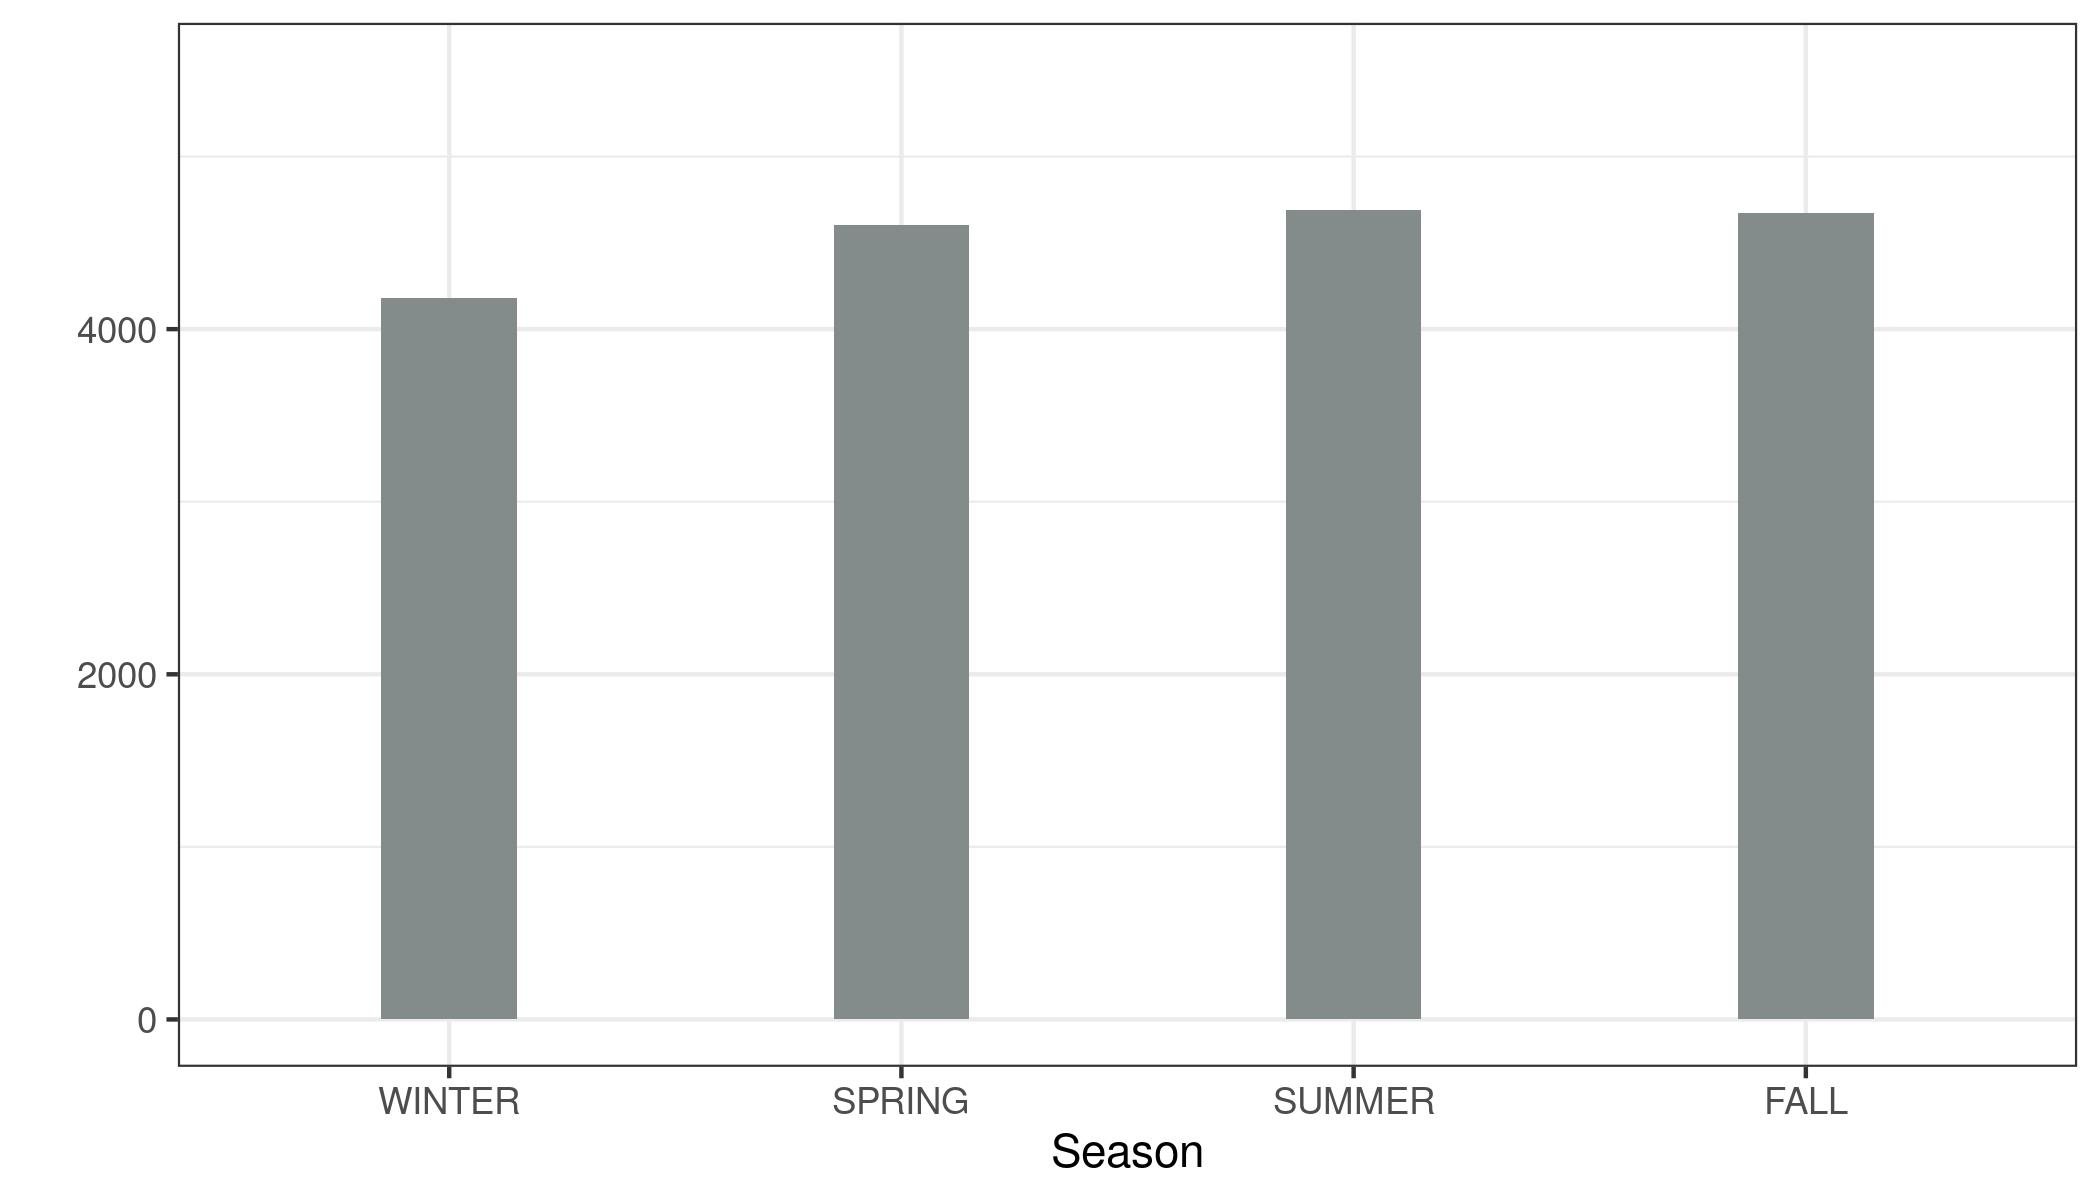
\includegraphics[width=.6\textwidth]{pdp-bike-cat-1}
      \caption{\footnotesize C. Molnar, IML book}
    \end{figure}
  \end{onlyenv}
\end{frame}

\begin{frame}
  \frametitle{Issues with PDPs}
  \begin{onlyenv}<1>
    \begin{itemize}
    \item Correlated features
      \begin{itemize}
      \item Example: $\text{price} = f(\text{num\_rooms}, \text{area})$
      \item To compute the effect of area for 40 $m^2$ we will use value 10 for
        the number of rooms (uncrealistic)
      \item As a result, we have a wrong estimation of the feature effect
      \end{itemize}
    \item Heterogeneous feature effects may be hidden by the use of average values
    \end{itemize}
  \end{onlyenv}
  \begin{onlyenv}<2>
    \begin{figure}
      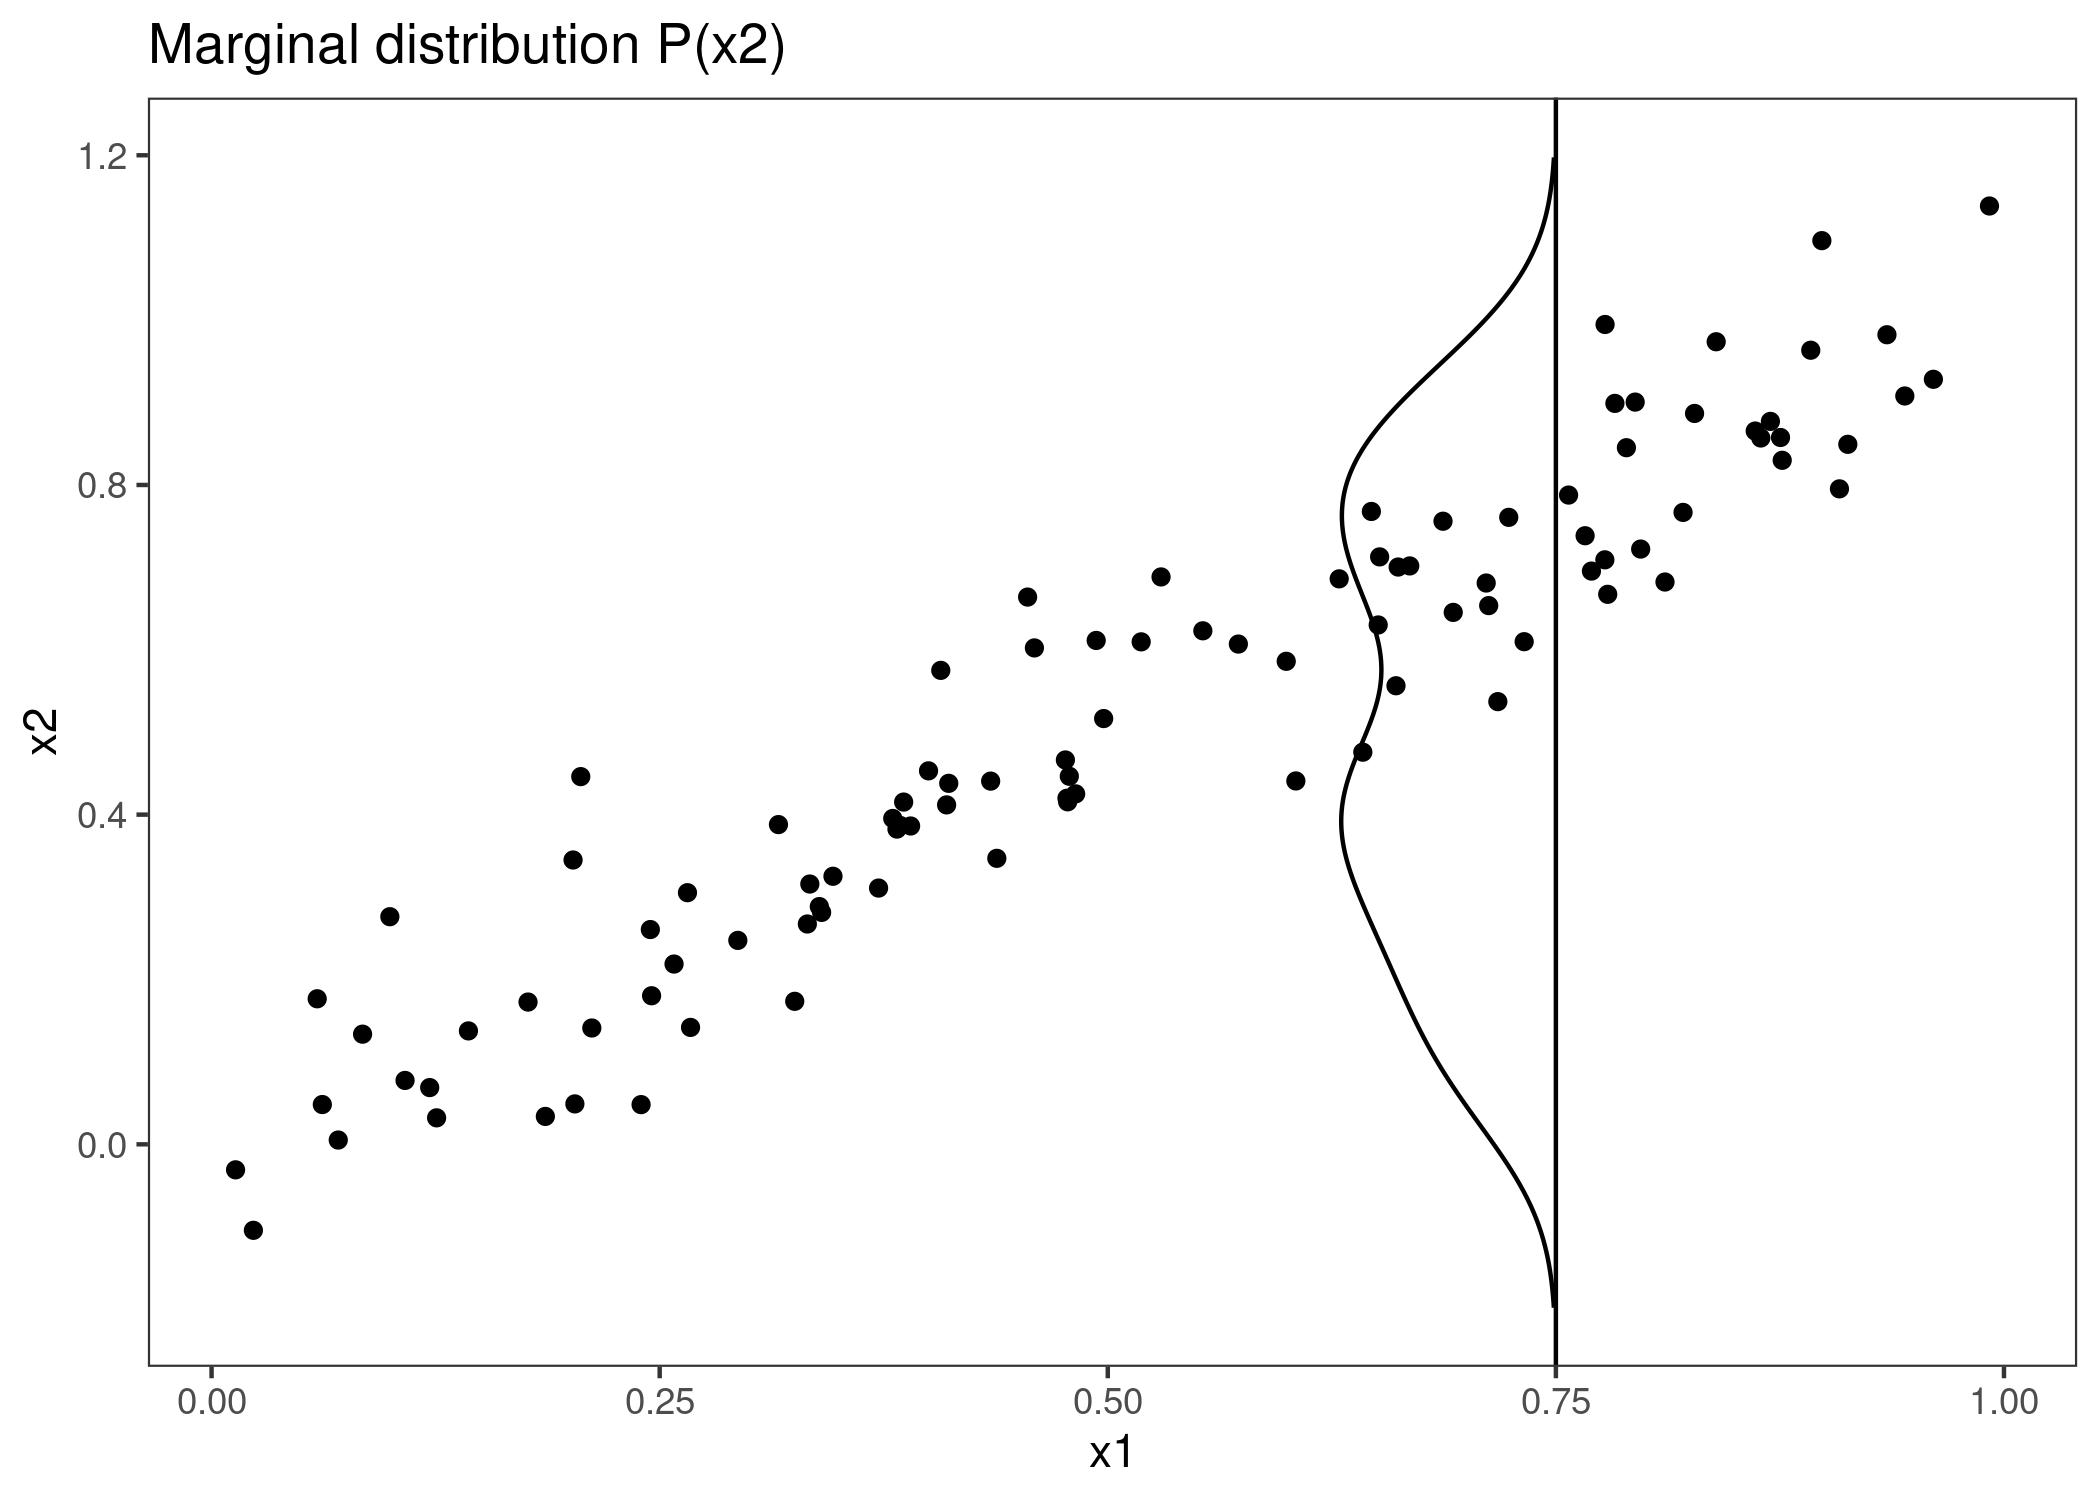
\includegraphics[width=.6\textwidth]{aleplot-motivation1-1}
      \caption{\footnotesize C. Molnar, IML book}
    \end{figure}
  \end{onlyenv}
\end{frame}

\begin{frame}
  \frametitle{MPlots}

  \begin{onlyenv}<1>
    We use the value of $x_s$ as a condition
    \begin{itemize}
    \item \(\Vx_c|x_s\): \(f(x_s) = \mathbb{E}_{\Vx_c|x_s}[f(x_s, \Vx_c)]\)
    \end{itemize}
  \end{onlyenv}
  \begin{onlyenv}<2>
    In the previous example
    \begin{figure}
      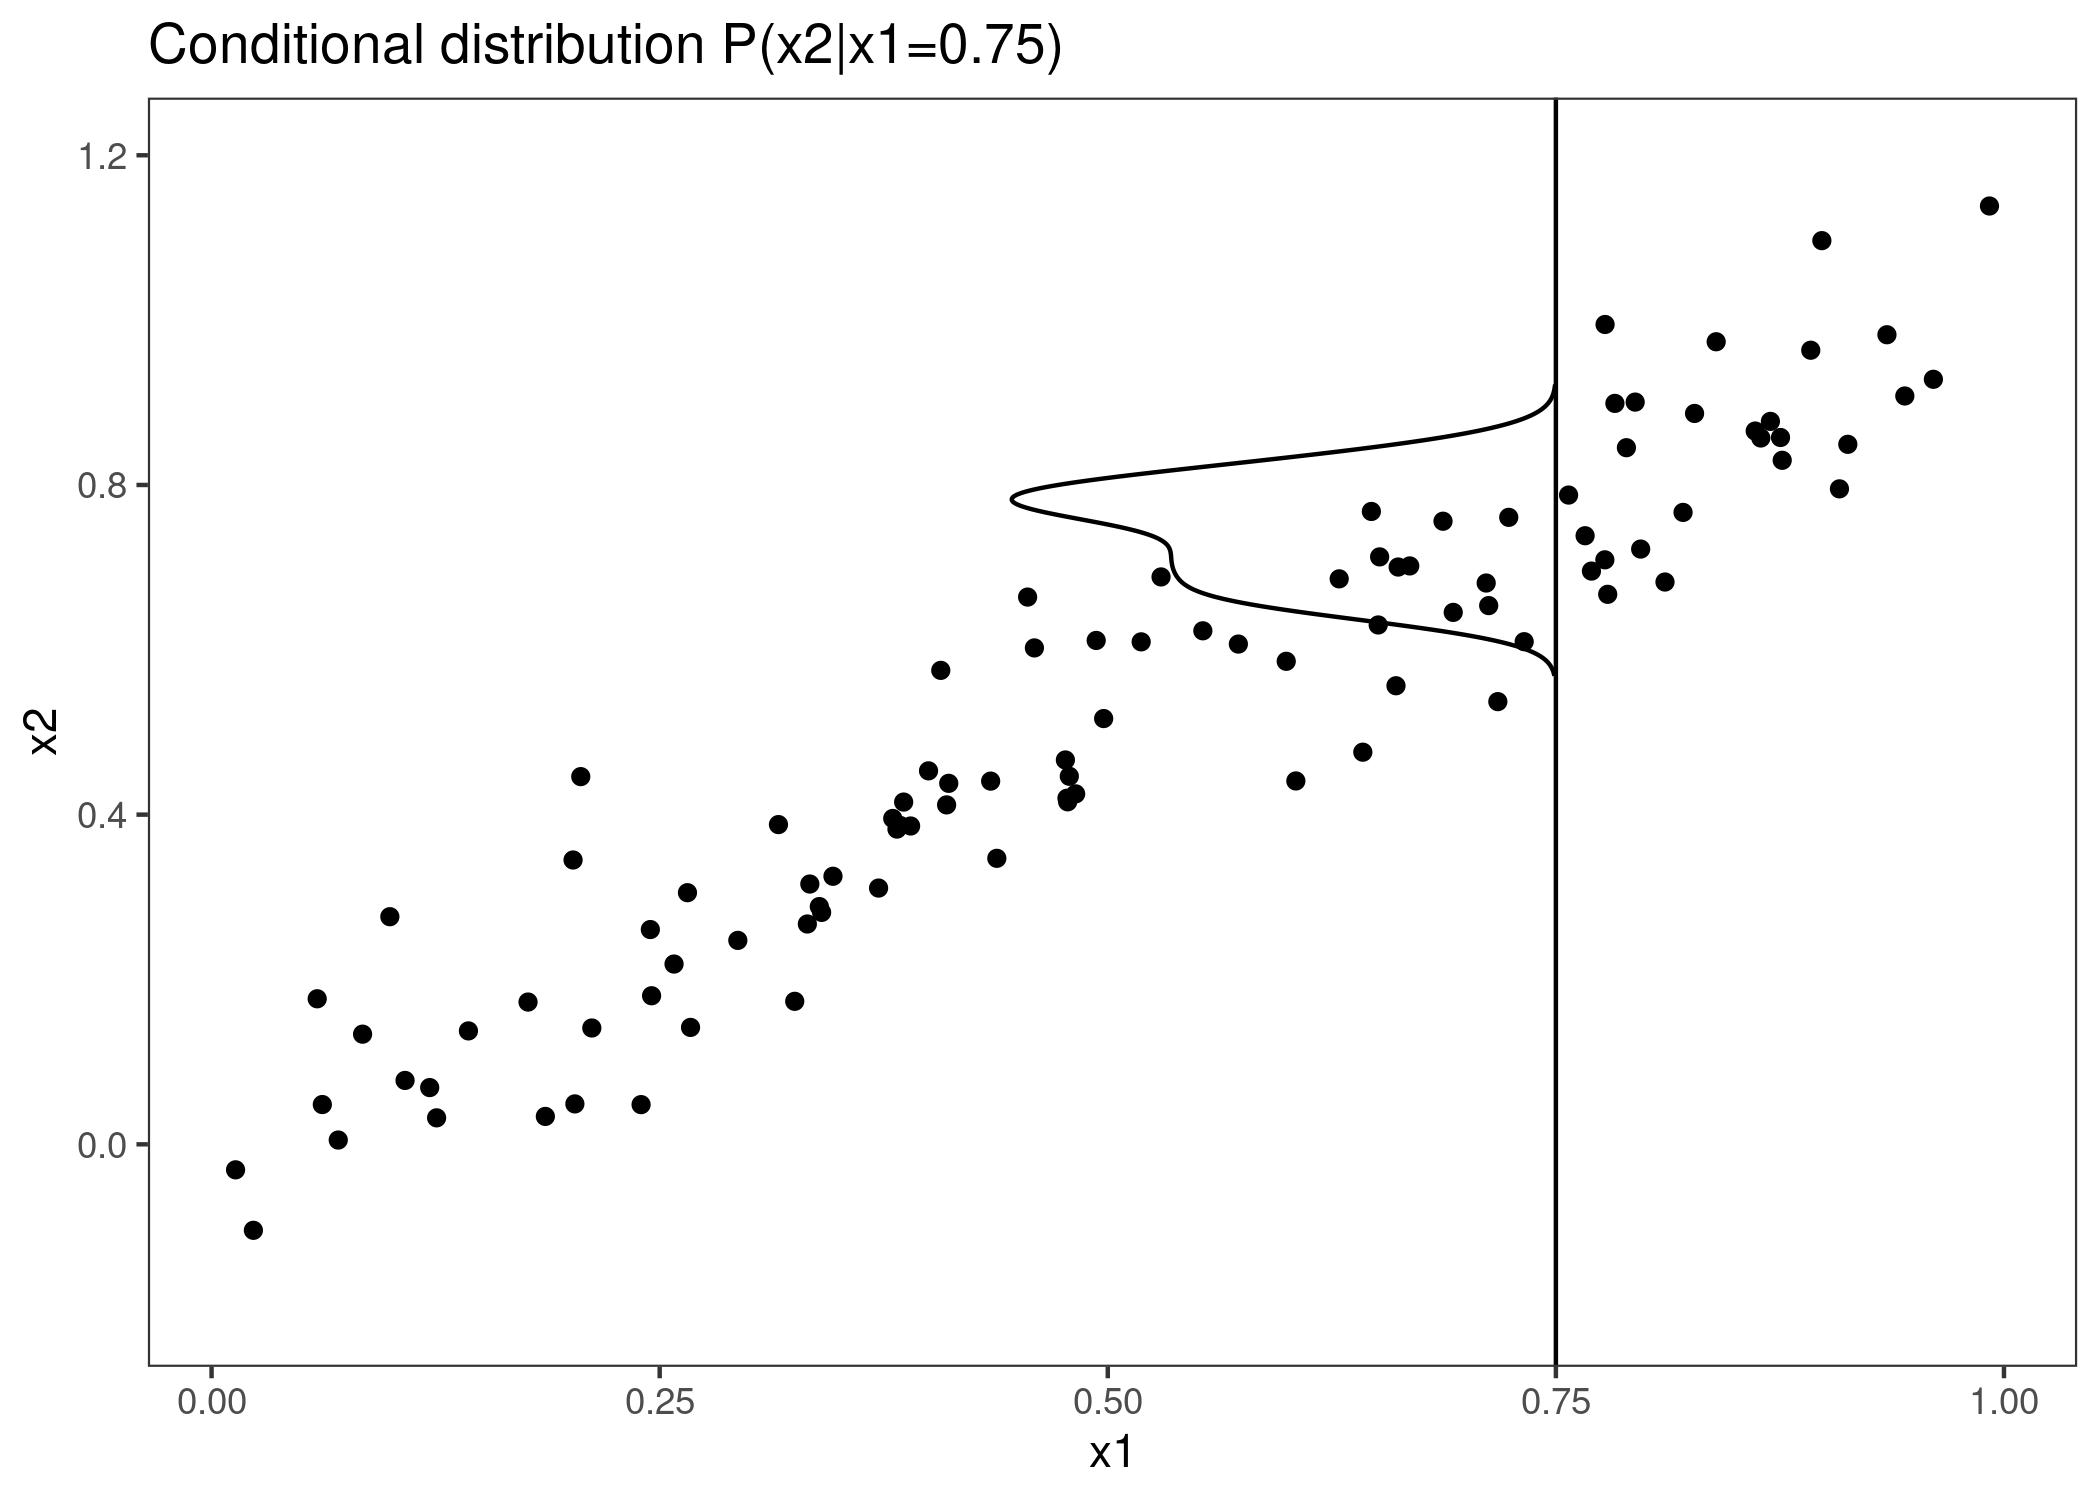
\includegraphics[width=.6\textwidth]{aleplot-motivation2-1}
      \caption{\footnotesize C. Molnar, IML book}
    \end{figure}
  \end{onlyenv}
\end{frame}

\begin{frame}
  \frametitle{Problems with M-Plots}
  \begin{itemize}
  \item The calculated effects result from the combination of all (correlated) features
  \item Real effect: \(x_{\mathtt{age}} = 50 \rightarrow 10\), \(x_{\mathtt{years\_contraceptives}} = 20 \rightarrow 10\)
  \item MPlot may estimate an effect of 17 for both
  \end{itemize}
\end{frame}

\begin{frame}
  \frametitle{Accumulated Local Effects (ALE)\footnote{D. Apley and
    J. Zhu. ``Visualizing the effects of predictor variables in black box
    supervised learning models.'' Journal of the Royal Statistical Society:
    Series B (Statistical Methodology) 82.4 (2020): 1059-1086.}}

  \begin{itemize}
  \item Resolves problems that result from the feature correlation by computing
    differences over a (small) window
  \item \(f(x_s) = \int_{x_{min}}^{x_s}\mathbb{E}_{\Vx_c|z}[ \frac{\partial f}{\partial x_s}(z, \Vx_c)] \partial z\)
  \end{itemize}
\end{frame}

\begin{frame}
  \frametitle{ALE approximation}
  ALE definition: \( f(x_s) = \int_{x_{s, min}}^{x_s}\mathbb{E}_{\Vx_c|z}[ \frac{\partial f}{\partial x_s}(z, \Vx_c)] \partial z \)
  % \noindent\makebox[\linewidth]{\rule{\paperwidth}{0.4pt}}
  ALE approximation: \(f(x_s) = \sum\limits_{k=1}^{k_x}
  \underbrace{\frac{1}{|\mathcal{S}_k|} \sum_{i:\Vx^i \in \mathcal{S}_k}
    \underbrace{[f(z_k, \Vx^i_c) - f(z_{k-1}, \Vx^i_c)]}_{\text{point
        effect}}}_{\text{bin effect}} \) 

  \begin{figure}[ht]
    \centering
    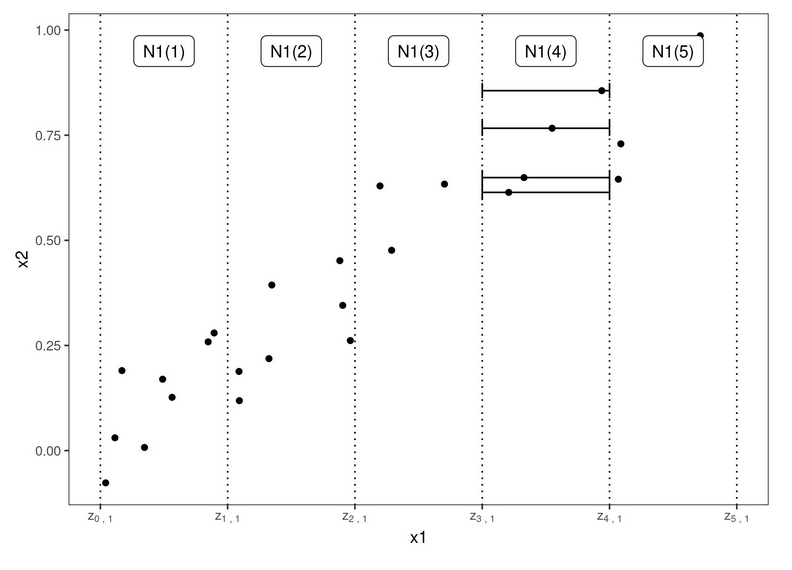
\includegraphics[width=0.5\textwidth]{./figures/ale_bins_iml.png}
    \caption{\footnotesize C. Molnar, IML book}
  \end{figure}

  \noindent\makebox[\linewidth]{\rule{\paperwidth}{0.4pt}}
  The number of bins (parameter \(K\)) is critical!
\end{frame}

\begin{frame}
  \frametitle{ALE plots - examples}
  \begin{onlyenv}<1>
    \begin{figure}
      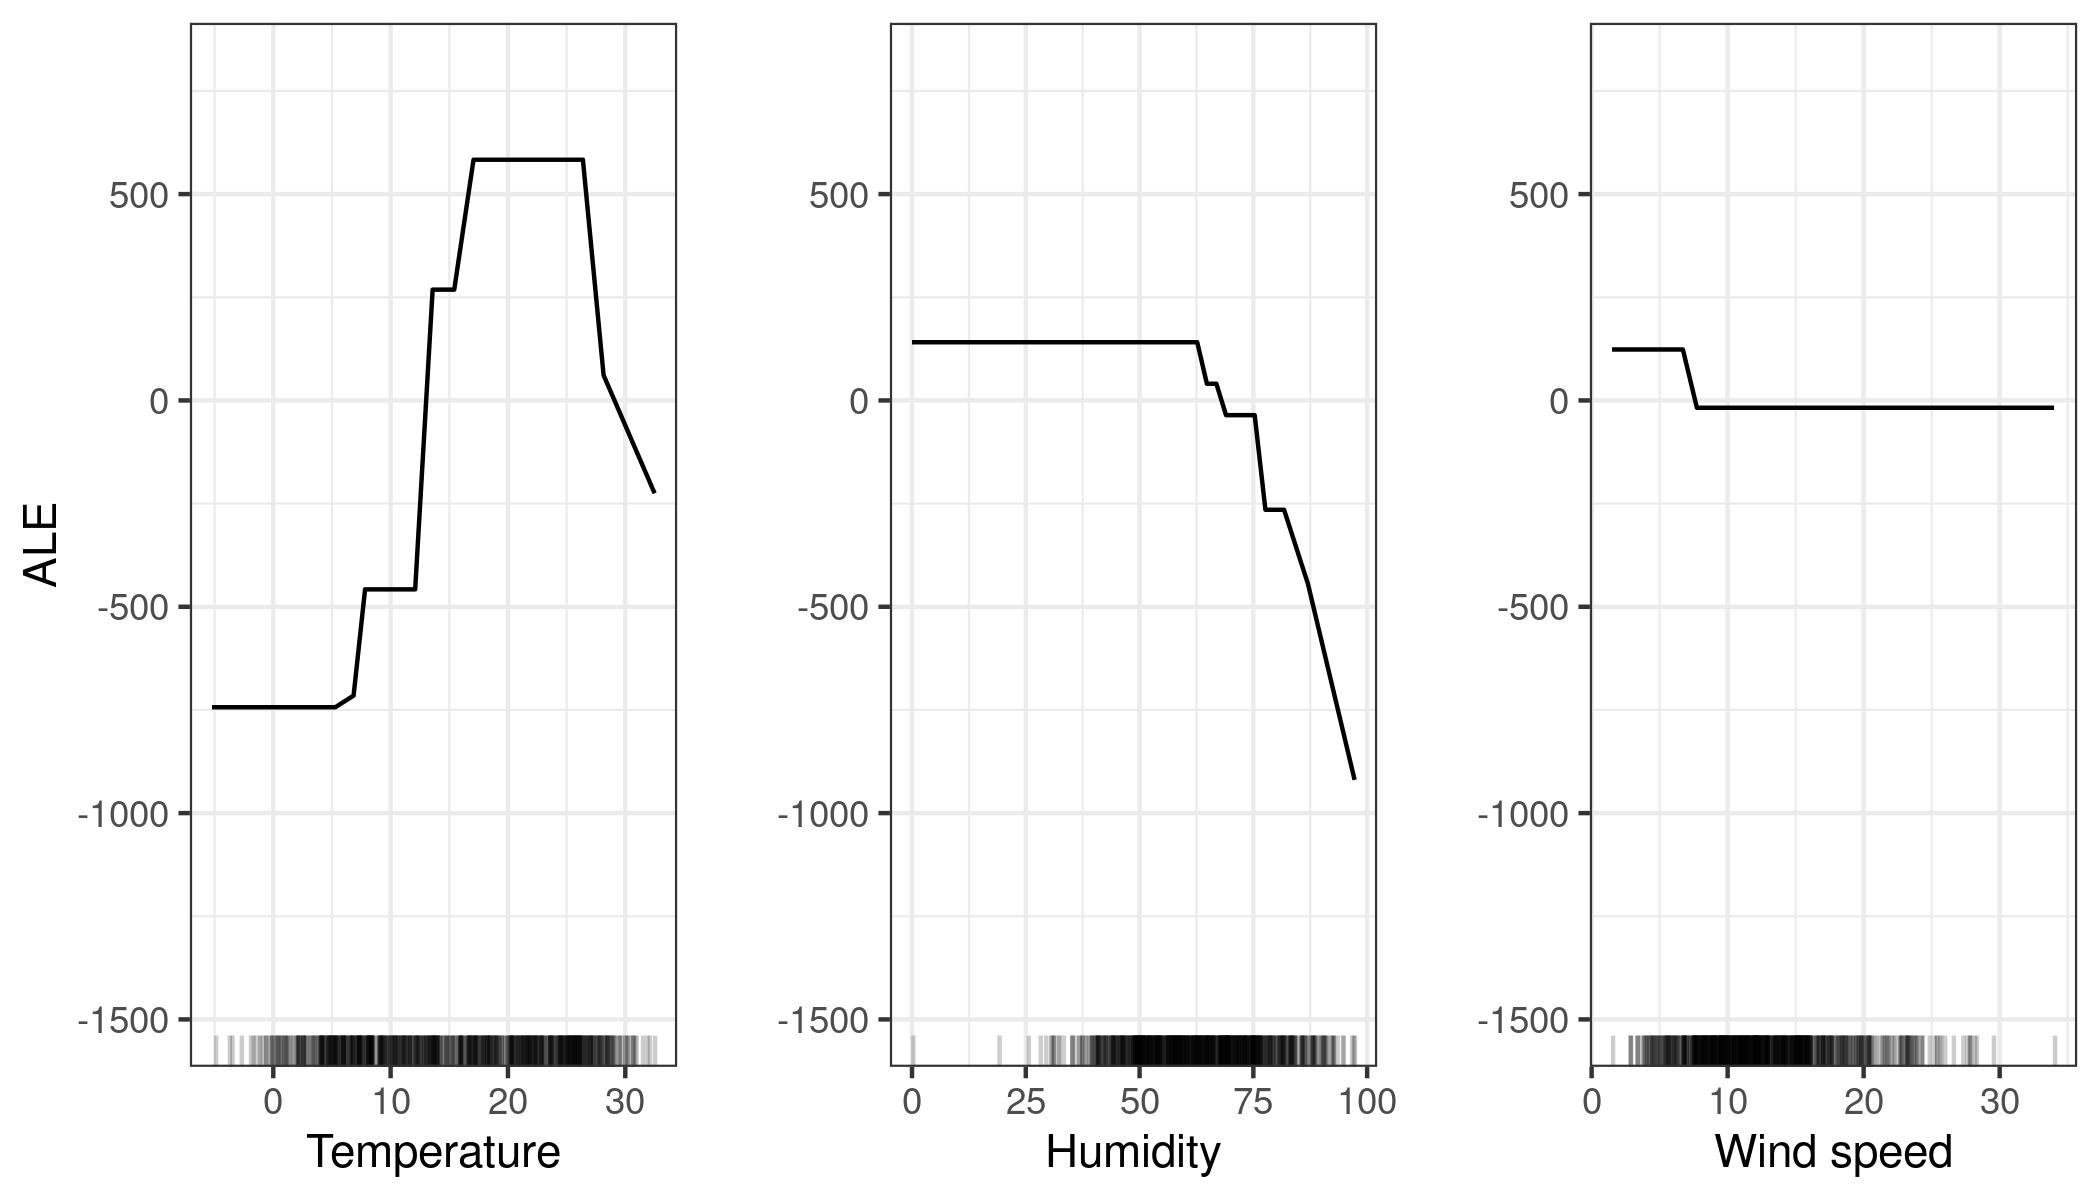
\includegraphics[width=.6\textwidth]{ale-bike-1}
      \caption{\footnotesize C. Molnar, IML book}
    \end{figure}
  \end{onlyenv}
  \begin{onlyenv}<2>
    \begin{figure}
      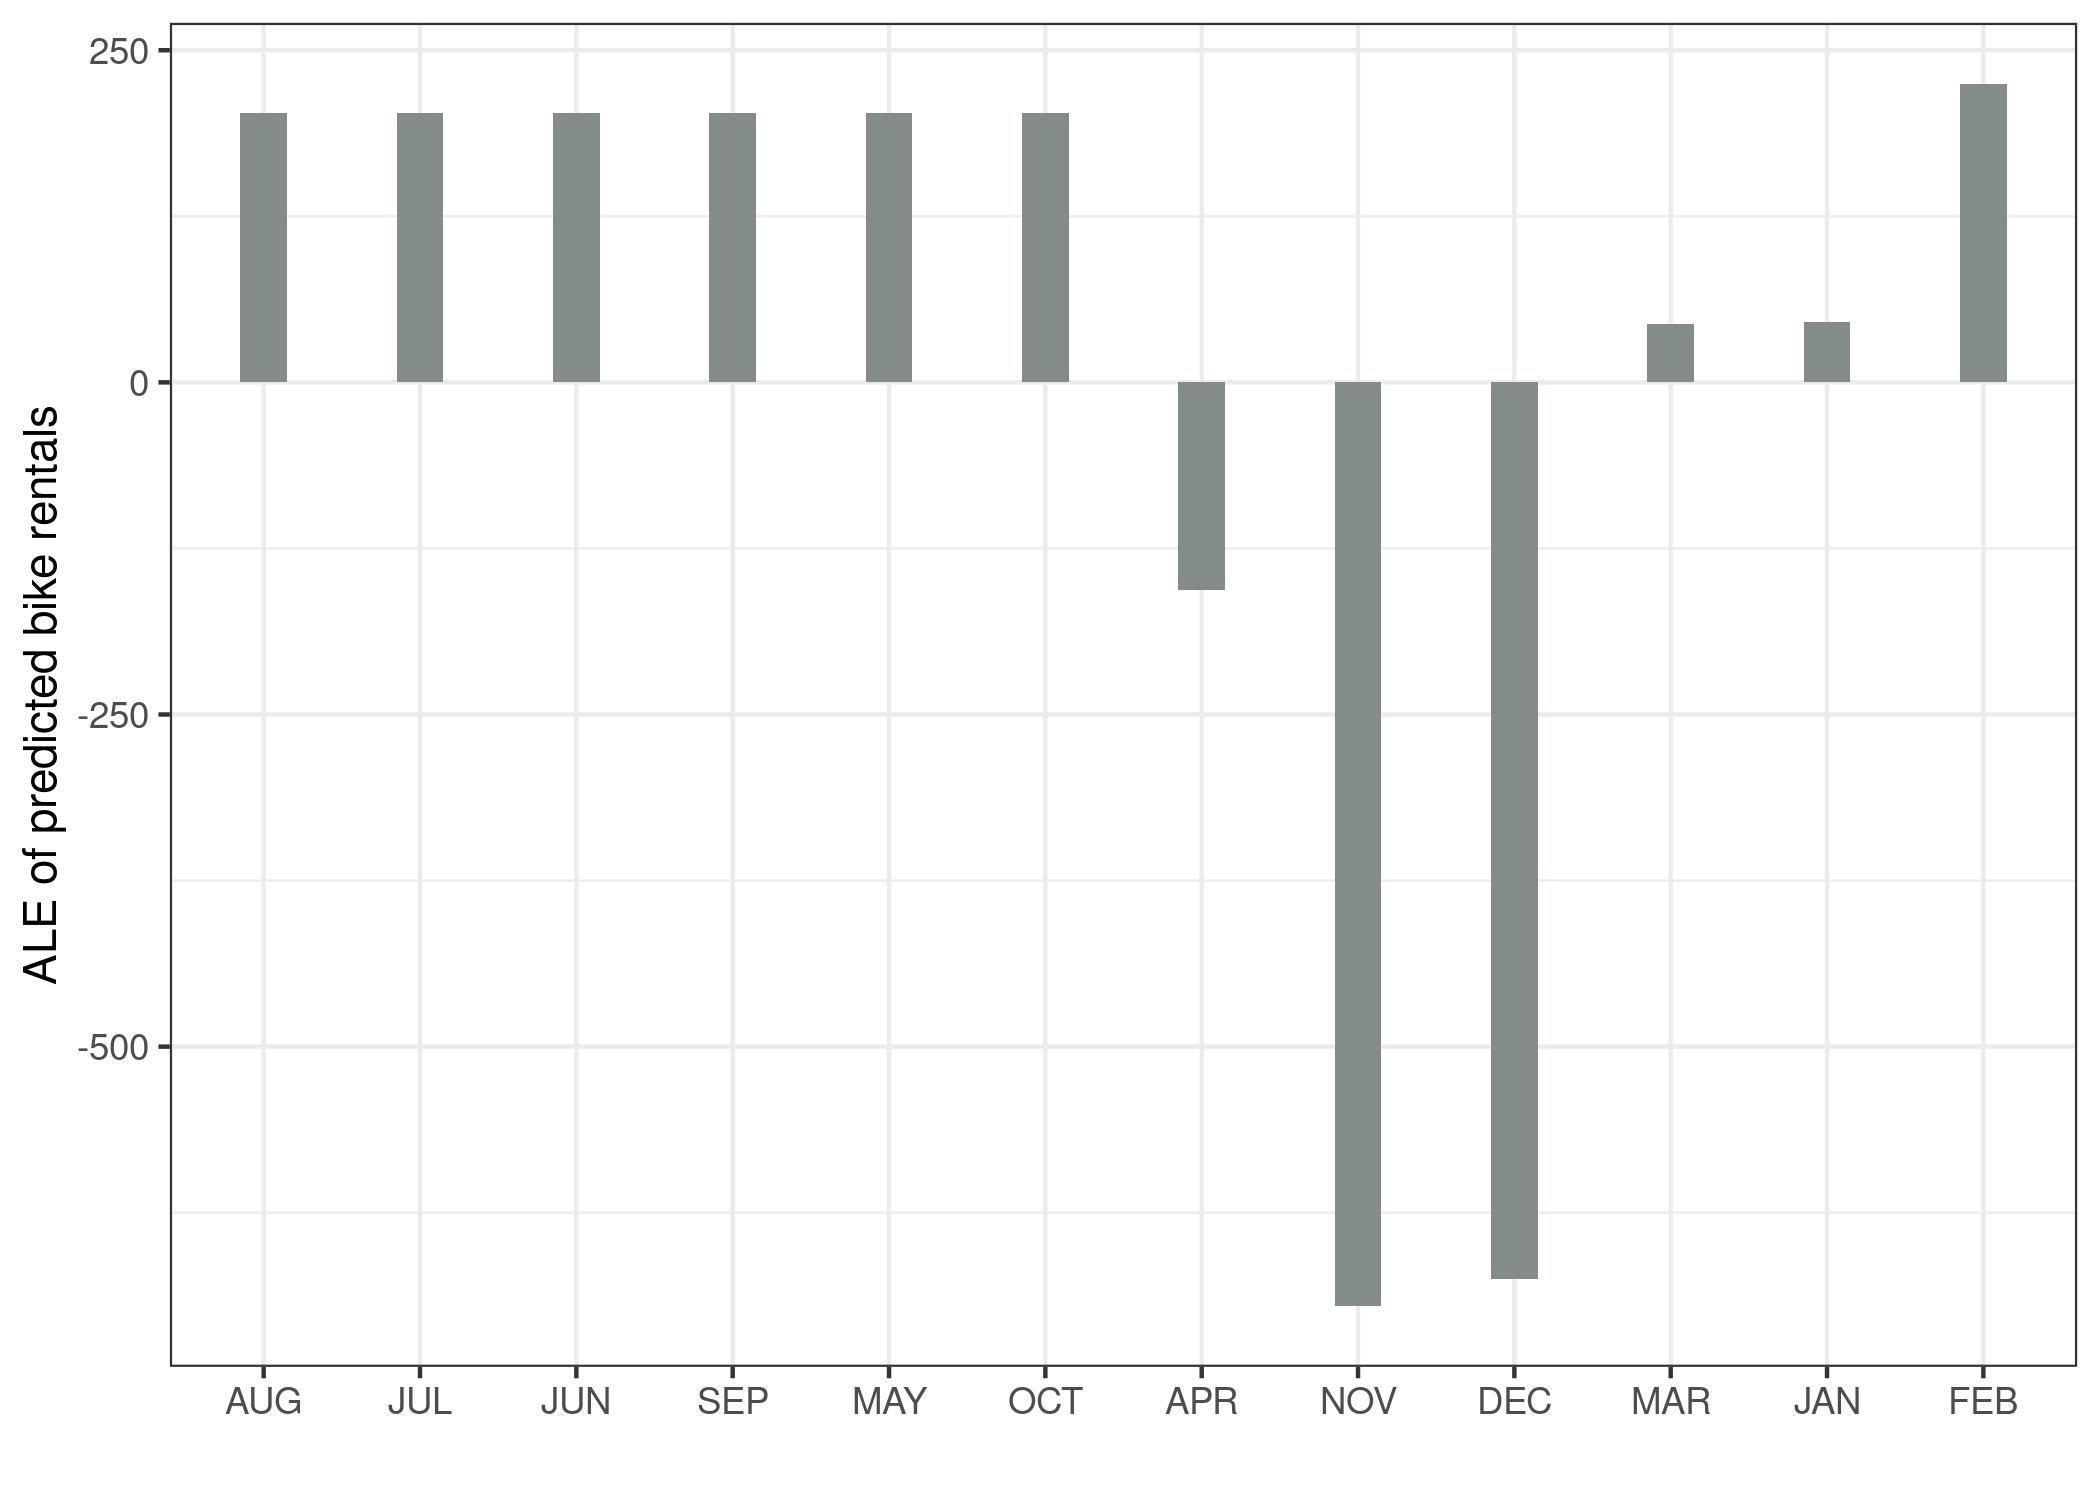
\includegraphics[width=.6\textwidth]{ale-bike-cat-1}
      \caption{\footnotesize C. Molnar, IML book}
    \end{figure}
  \end{onlyenv}
\end{frame}

\section{DALE}

\begin{frame}[plain,c]
  \Large{V. Gkolemis, T. Dalamagas, C. Diou, ``DALE: Differential Accumulated
  Local Effects for efficient and accurate global explanations'', ACML, 2022}

  \vspace{1cm}
  Most of the work done by this guy:\\
  \begin{figure}
    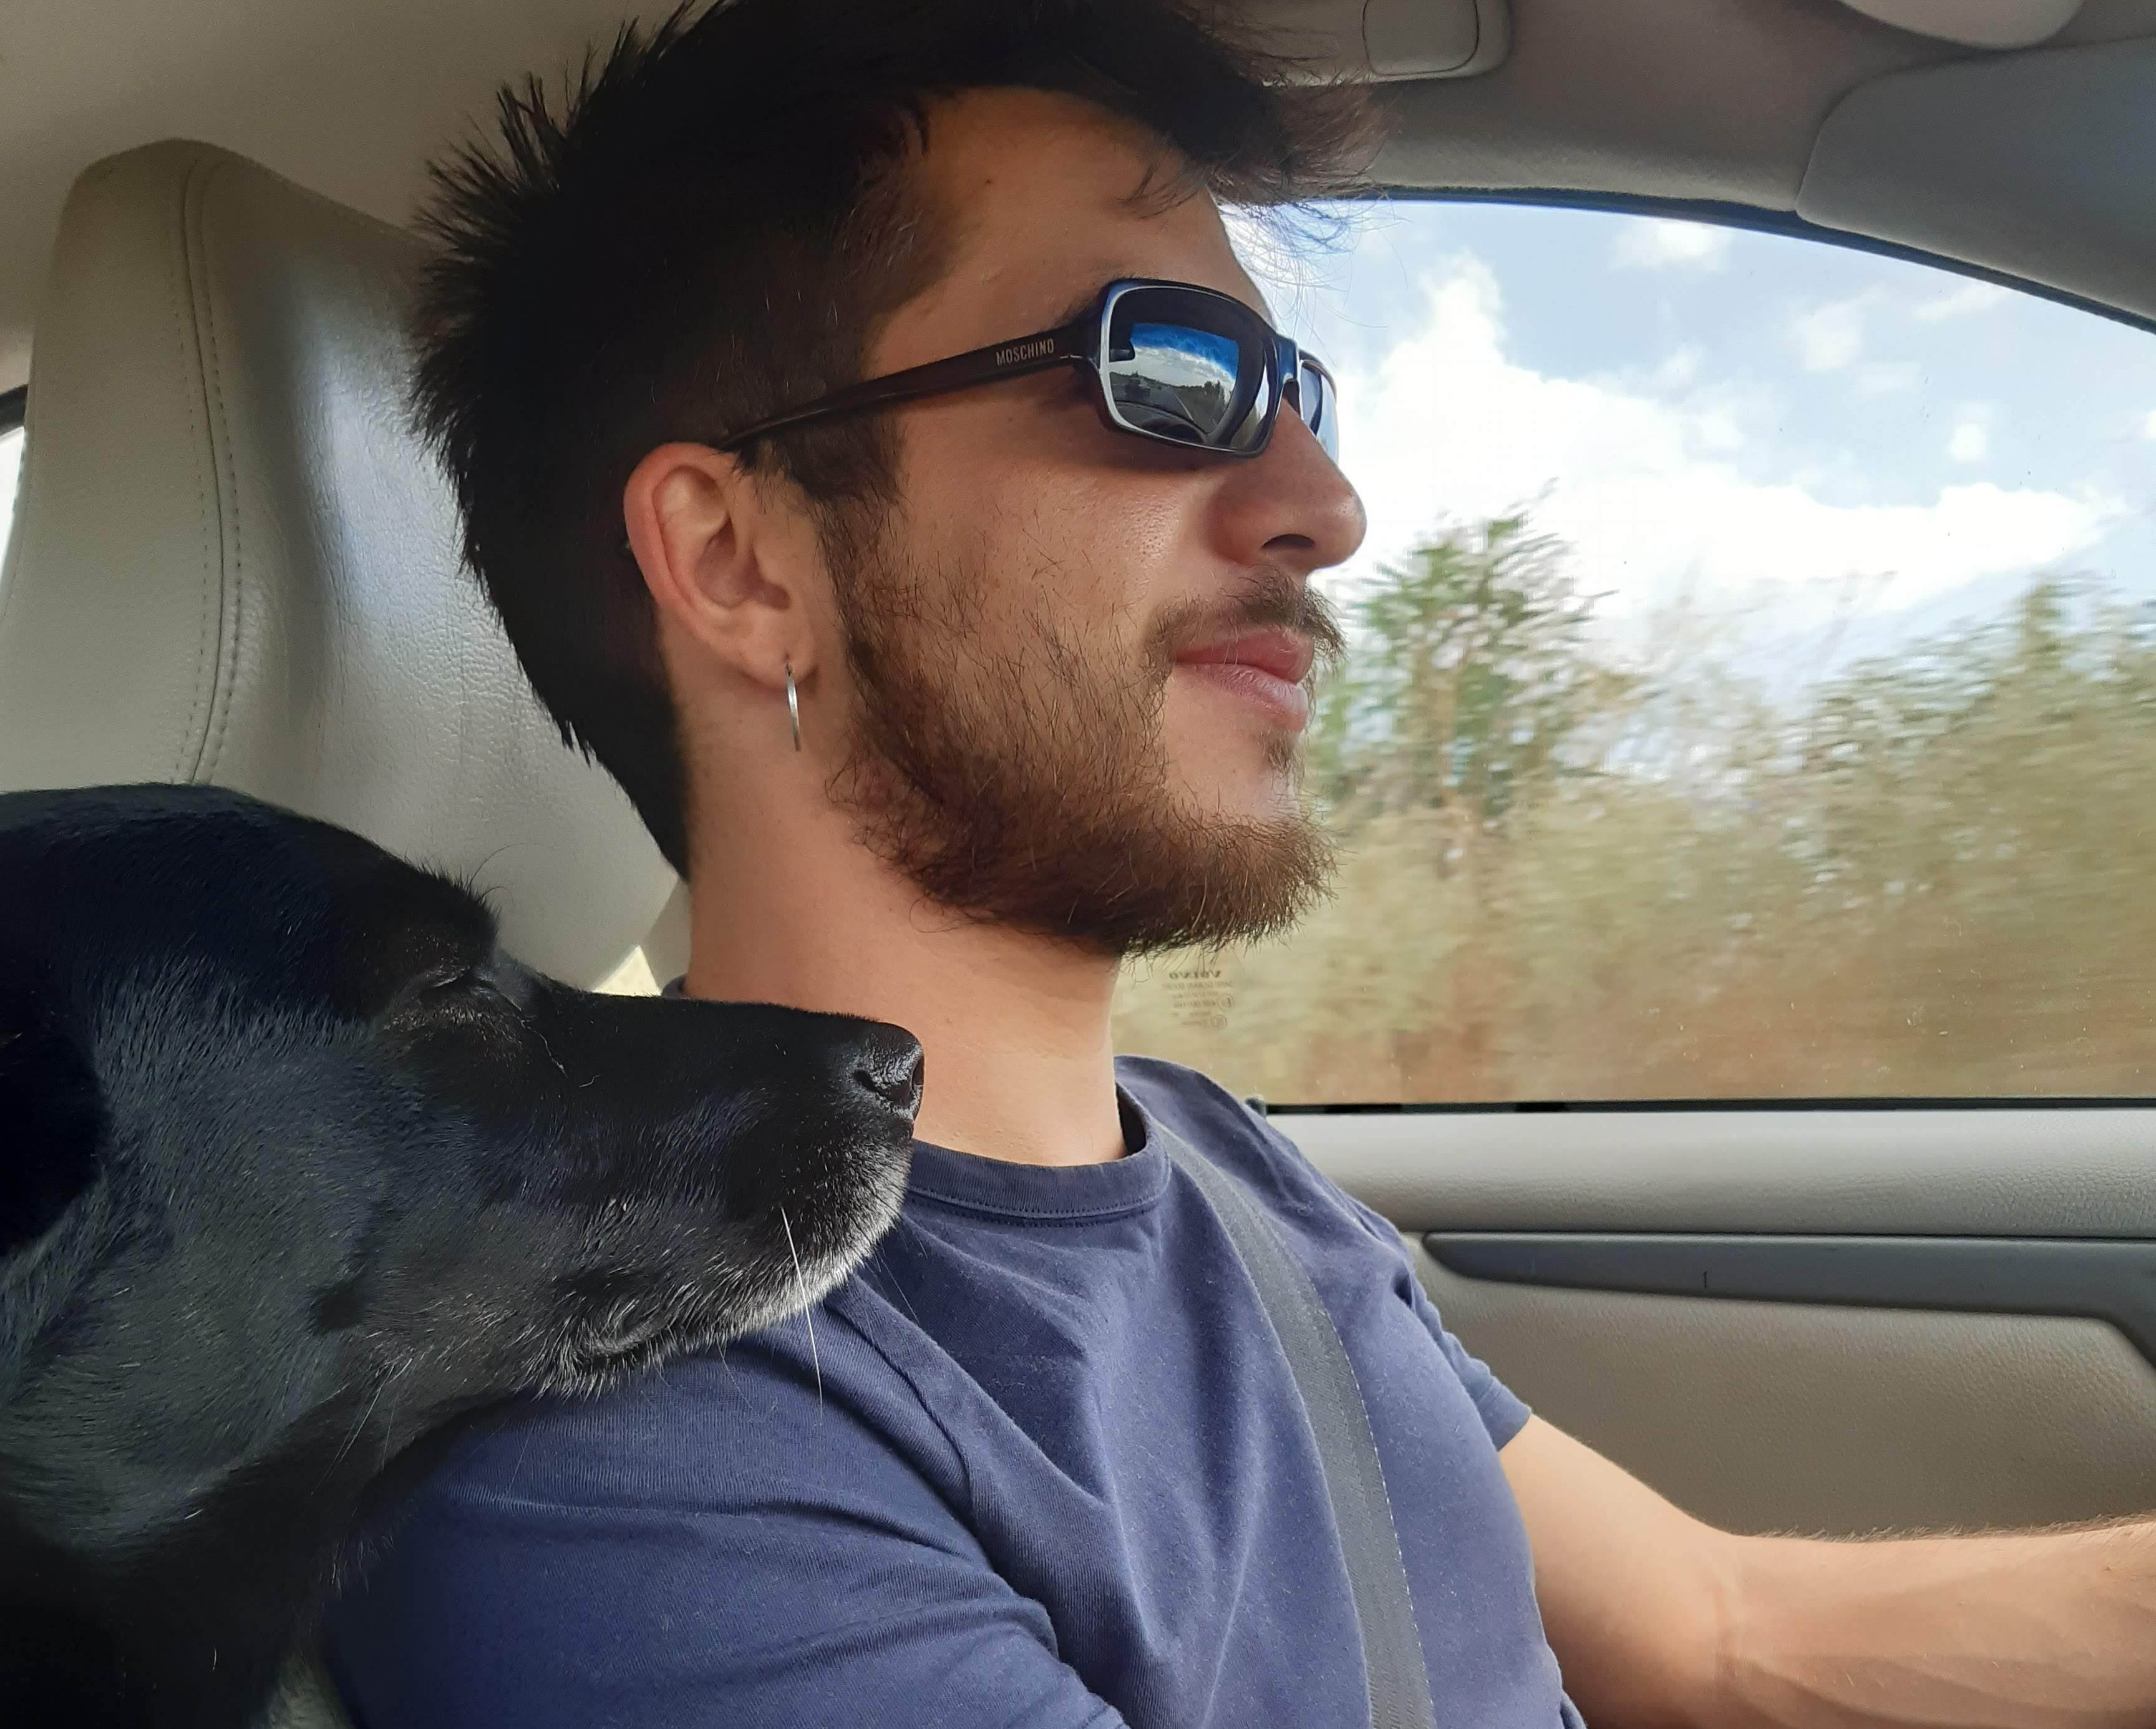
\includegraphics[width=.2\textwidth]{gkolemis}
  \end{figure}
\end{frame}

\begin{frame}
  \frametitle{ALE approximation - weaknesses}

  \begin{equation*}
    f(x_s) = \sum_k^{k_x} \underbrace{\frac{1}{|\mathcal{S}_k|} \sum_{i:\xb^i
        \in \mathcal{S}_k} \underbrace{[f(z_k, \Vx^i_c) - f(z_{k-1},
          \Vx^i_c)]}_{\text{point effect}}}_{\text{bin effect}}
  \end{equation*}

  \begin{itemize}
  \item Point Effect \(\Rightarrow\) evaluation \alert{at bin limits}
    \begin{itemize}
    \item 2 evaluations of \(f\) per point \( \rightarrow \) slow
    \item change bin limits, pay again \(2*N\) evaluations of \(f\) \( \rightarrow\) restrictive
    \item broad bins may create out of distribution (OOD) samples \( \rightarrow\) not-robust in wide bins
    \end{itemize}
  \end{itemize}

\end{frame}


\begin{frame}
  \frametitle{Our proposal: Differential ALE}
  \begin{equation*}
    f(x_s) = \Delta x \sum_k^{k_x} \underbrace{\frac{1}{|\mathcal{S}_k|}
      \sum_{i:\xb^i \in \mathcal{S}_k} \underbrace{[\frac{\partial f(x_s^i, \Vx^i_c)}{\partial
            x_s}]}_{\text{\alert{point effect}}}}_{\text{bin effect}}
  \end{equation*}

  \begin{itemize}
  \item Point Effect \(\Rightarrow\) evaluation \alert{on instances}
    \begin{itemize}
    \item Fast \( \rightarrow \) use of auto-differentiation, all derivatives in a single pass
    \item Versatile \( \rightarrow\) point effects computed once, change bins without cost
    \item Secure \( \rightarrow\) does not create artificial instances
    \end{itemize}
  \end{itemize}

  For \alert{differentiable} models, DALE resolves ALE weaknesses
\end{frame}



% chapter 1
\section{DALE vs ALE}

\subsection{Dale is faster and versatile}

\begin{frame}
  \frametitle{DALE is faster and versatile - theory}
  \[f(x_s) = \Delta x \sum_k^{k_x} \underbrace{\frac{1}{|\mathcal{S}_k|} \sum_{i:\xb^i \in \mathcal{S}_k} \underbrace{[\frac{\partial f(x_s^i, \Vx^i_c)}{\partial x_s}]}_{\text{point effect}}}_{\text{bin effect}} \]

  \begin{itemize}
  \item Faster
    \begin{itemize}
    \item gradients wrt all features \(\nabla_{\Vx} f(\Vx^i)\) in a single pass
    \item auto-differentiation must be available (deep learning)
    \end{itemize}
  \item Versatile
    \begin{itemize}
    \item Change bin limits, with near zero computational cost
    \end{itemize}

  \end{itemize}
  DALE is faster and allows redefining bin-limits
\end{frame}

\begin{frame}
  \frametitle{DALE is faster and versatile - Experiments}
  \begin{figure}[h]
    \centering
    \resizebox{.4\columnwidth}{!}{% This file was created with tikzplotlib v0.10.1.
\begin{tikzpicture}

\definecolor{darkgray176}{RGB}{176,176,176}
\definecolor{dodgerblue}{RGB}{30,144,255}
\definecolor{lightgray204}{RGB}{204,204,204}

\begin{axis}[
legend cell align={left},
legend style={
  fill opacity=0.8,
  draw opacity=1,
  text opacity=1,
  at={(0.03,0.97)},
  anchor=north west,
  draw=lightgray204
},
tick align=outside,
tick pos=left,
title={DALE vs ALE: Light setup},
x grid style={darkgray176},
xlabel={\(\displaystyle D\)},
xmin=0.25, xmax=104.75,
xtick style={color=black},
y grid style={darkgray176},
ylabel={time (seconds)},
ymin=-0.118335867500491, ymax=2.74596303149951,
ytick style={color=black}
]
\addplot [semithick, red, dashed, mark=*, mark size=3, mark options={solid}]
table {%
5 0.0118595361709595
10 0.0122641324996948
15 0.0128312110900879
20 0.0119729042053223
25 0.0144194364547729
50 0.0124425888061523
100 0.0135363340377808
};
\addlegendentry{$f(x)$}
\addplot [semithick, blue, dashed, mark=*, mark size=3, mark options={solid}]
table {%
5 0.0321429967880249
10 0.0295344591140747
15 0.0305428504943848
20 0.0298470258712769
25 0.0309284925460815
50 0.0336670875549316
100 0.032146692276001
};
\addlegendentry{$\mathbf{J}$}
\addplot [semithick, dodgerblue, dashed, mark=*, mark size=3, mark options={solid}]
table {%
5 0.130752086639404
10 0.275371313095093
15 0.398597836494446
20 0.496960043907166
25 0.623412370681763
50 1.27240407466888
100 2.61576771736145
};
\addlegendentry{$\hat{f}_{\mathtt{ALE}}$}
\addplot [semithick, black, dashed, mark=*, mark size=3, mark options={solid}]
table {%
5 0.0335890054702759
10 0.0366946458816528
15 0.0436010360717773
20 0.0414165258407593
25 0.0466822385787964
50 0.0650126934051514
100 0.0961912870407104
};
\addlegendentry{$\hat{f}_{\mathtt{DALE}}$}
\end{axis}

\end{tikzpicture}
}
    \resizebox{.43\columnwidth}{!}{% This file was created with tikzplotlib v0.10.1.
\begin{tikzpicture}

\definecolor{darkgray176}{RGB}{176,176,176}
\definecolor{dodgerblue}{RGB}{30,144,255}
\definecolor{lightgray204}{RGB}{204,204,204}

\begin{axis}[
legend cell align={left},
legend style={
  fill opacity=0.8,
  draw opacity=1,
  text opacity=1,
  at={(0.03,0.97)},
  anchor=north west,
  draw=lightgray204
},
tick align=outside,
tick pos=left,
title={DALE vs ALE: Heavy setup},
x grid style={darkgray176},
xlabel={\(\displaystyle D\)},
xmin=0.25, xmax=104.75,
xtick style={color=black},
y grid style={darkgray176},
ylabel={time (seconds)},
ymin=-38.1810145603003, ymax=867.056094992299,
ytick style={color=black}
]
\addplot [semithick, red, dashed, mark=*, mark size=3, mark options={solid}]
table {%
5 3.13364505767822
10 3.24496150016785
15 6.86045789718628
20 2.96612668037415
25 3.05197858810425
50 3.02510833740234
100 3.71672296524048
};
\addlegendentry{$f(x)$}
\addplot [semithick, blue, dashed, mark=*, mark size=3, mark options={solid}]
table {%
5 8.88222980499268
10 8.82908821105957
15 18.4925575256348
20 8.51719951629639
25 13.5228071212769
50 12.4858655929565
100 8.59451198577881
};
\addlegendentry{$\mathbf{J}$}
\addplot [semithick, dodgerblue, dashed, mark=*, mark size=3, mark options={solid}]
table {%
5 31.310697555542
10 74.1438674926758
15 116.133689880371
20 160.465118408203
25 195.409912109375
50 391.950622558594
100 825.908935546875
};
\addlegendentry{$\hat{f}_{\mathtt{ALE}}$}
\addplot [semithick, black, dashed, mark=*, mark size=3, mark options={solid}]
table {%
5 8.83595371246338
10 9.03882694244385
15 9.21370220184326
20 8.9499044418335
25 16.3313121795654
50 16.7110271453857
100 10.0340776443481
};
\addlegendentry{$\hat{f}_{\mathtt{DALE}}$}
\end{axis}

\end{tikzpicture}
}
    \caption[Case-1-fig-1]{Light setup; small dataset \((N=10^2\) instances), light \(f\). Heavy setup; big dataset (\(N=10^5\) instances), heavy \(f\)}
    \label{fig:case-1-plots-1}
  \end{figure}

  \noindent\makebox[\linewidth]{\rule{\paperwidth}{0.4pt}}
  DALE considerably accelerates the estimation
\end{frame}


\subsection{DALE is more Accurate}

\begin{frame}
  \frametitle{DALE uses on-distribution samples - Theory}
  \[f(x_s) = \sum_k^{k_x} \underbrace{\frac{1}{|\mathcal{S}_k|}
    \sum_{i:\xb^i \in \mathcal{S}_k} \underbrace{[\frac{\partial
          f(x_s^i, \Vx^i_c)}{\partial x_s}]}_{\text{point
        effect}}}_{\text{bin effect}} \]

  \begin{itemize}
  \item point effect \alert{independent} of bin limits
    \begin{itemize}
    \item \(\frac{\partial f(x_s^i, \Vx^i_c)}{\partial x_s}\)
      computed on real instances \(\Vx^i = (x_s^i, \Vx_c^i)\)
    \end{itemize}
  \item bin limits affect only the \alert{resolution} of the plot
    \begin{itemize}
    \item wide bins \(\rightarrow\) low resolution plot, bin
      estimation from more points
    \item narrow bins \(\rightarrow\) high resolution plot, bin
      estimation from less points
    \end{itemize}
  \end{itemize}
  DALE enables wide bins without creating out of distribution instances
\end{frame}


\begin{frame}
  \frametitle{DALE uses on-distribution samples - Experiments}
  \begin{columns}
    \begin{column}{0.5\textwidth}
      \[ f(x_1, x_2, x_3) = x_1x_2 + x_1x_3 \: \textcolor{red}{ \pm \: g(x)}\]
      \[ x_1 \in [0,10], x_2 \sim x_1 + \epsilon, x_3 \sim \mathcal{N}(0, \sigma^2) \]
      \[ f_{\mathtt{ALE}}(x_1) = \frac{x_1^2}{2} \]
      \begin{itemize}
      \item point effects affected by \((x_1x_3)\) (\(\sigma\) is large)
      \item bin estimation is noisy (samples are few)
      \end{itemize}
    \end{column}
    \begin{column}{0.5\textwidth}
      \begin{center}
        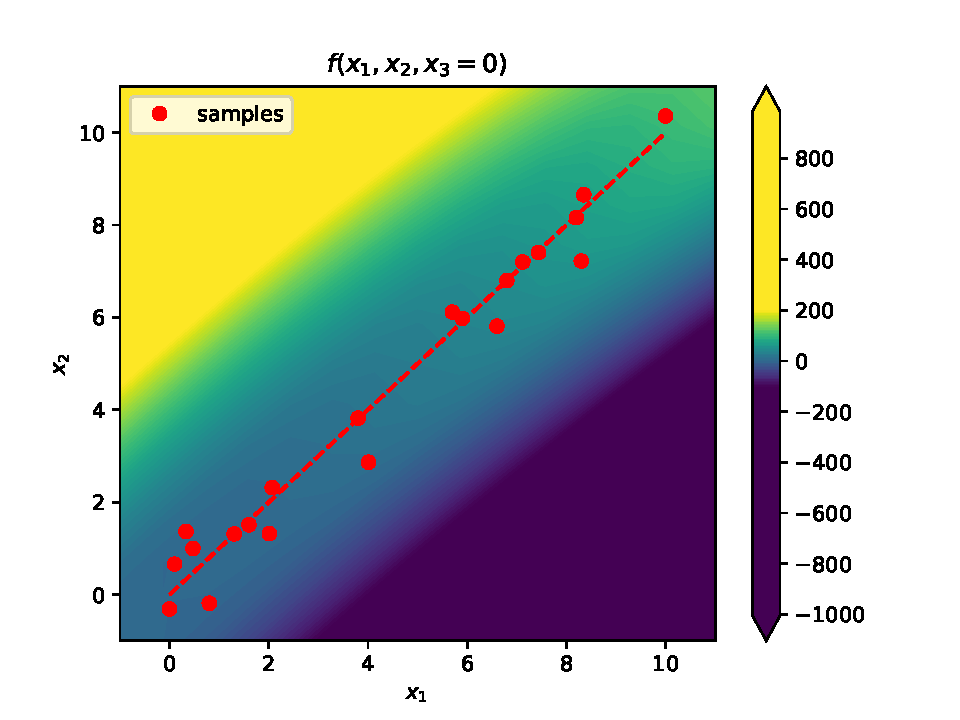
\includegraphics[width=\textwidth]{./figures/f_plot.pdf}
      \end{center}
    \end{column}
  \end{columns}
  Intuition: we need wider bins (more samples per bin)
\end{frame}


\begin{frame}
  \frametitle{DALE vs ALE - 40 Bins}
  \begin{figure}
    \centering
    \includegraphics<1>[width=0.6\textwidth]{./figures/bin_splitting_40_bins.pdf}
    \includegraphics<2>[width=.49\textwidth]{./figures/dale_40_bins.pdf}
    \includegraphics<2>[width=.49\textwidth]{./figures/ale_40_bins.pdf}
  \end{figure}
  \begin{itemize}
  \item DALE: on-distribution, noisy bin effect \(\rightarrow\) \textcolor{red}{poor estimation}
  \item ALE: on-distribution, noisy bin effect \(\rightarrow\) \textcolor{red}{poor estimation}
  \end{itemize}
\end{frame}

\begin{frame}
  \frametitle{DALE vs ALE - 20 Bins}
  \begin{figure}[ht]
    \centering
    \includegraphics<1>[width=0.6\textwidth]{./figures/bin_splitting_20_bins.pdf}
    \includegraphics<2>[width=0.49\textwidth]{./figures/dale_20_bins.pdf}
    \includegraphics<2>[width=0.49\textwidth]{./figures/ale_20_bins.pdf}
  \end{figure}
  \begin{itemize}
  \item DALE: on-distribution, noisy bin effect \(\rightarrow\) \textcolor{red}{poor estimation}
  \item ALE: on-distribution, noisy bin effect \(\rightarrow\) \textcolor{red}{poor estimation}
  \end{itemize}
\end{frame}


\begin{frame}
  \frametitle{DALE vs ALE - 10 Bins}
  \begin{figure}[ht]
    \centering
    \includegraphics<1>[width=0.6\textwidth]{./figures/bin_splitting_10_bins.pdf}
    \includegraphics<2>[width=0.49\textwidth]{./figures/dale_10_bins.pdf}
    \includegraphics<2>[width=0.49\textwidth]{./figures/ale_10_bins.pdf}
  \end{figure}
  \begin{itemize}
  \item DALE: on-distribution, noisy bin effect \(\rightarrow\) \textcolor{red}{poor estimation}
  \item ALE: starts being OOD, noisy bin effect \(\rightarrow\) \textcolor{red}{poor estimation}
  \end{itemize}
\end{frame}

\begin{frame}
  \frametitle{DALE vs ALE - 5 Bins}
  \begin{figure}[ht]
    \centering
    \includegraphics<1>[width=0.6\textwidth]{./figures/bin_splitting_5_bins.pdf}
    \includegraphics<2>[width=0.49\textwidth]{./figures/dale_5_bins.pdf}
    \includegraphics<2>[width=0.49\textwidth]{./figures/ale_5_bins.pdf}
  \end{figure}
  \begin{itemize}
  \item DALE: on-distribution, robust bin effect \(\rightarrow\) \textcolor{green}{good estimation}
  \item ALE: completely OOD, robust bin effect \(\rightarrow\) \textcolor{red}{poor estimation}
  \end{itemize}
\end{frame}

\begin{frame}
  \frametitle{DALE vs ALE - 3 Bins}
  \begin{figure}[ht]
    \centering
    \includegraphics<1>[width=0.6\textwidth]{./figures/bin_splitting_3_bins.pdf}
    \includegraphics<2>[width=0.49\textwidth]{./figures/dale_3_bins.pdf}
    \includegraphics<2>[width=0.49\textwidth]{./figures/ale_3_bins.pdf}
  \end{figure}
  \begin{itemize}
  \item DALE: on-distribution, robust bin effect \(\rightarrow\) \textcolor{green}{good estimation}
  \item ALE: completely OOD, robust bin effect \(\rightarrow\) \textcolor{red}{poor estimation}
  \end{itemize}
\end{frame}


\begin{frame}
  \frametitle{Real Dataset Experiments - Efficiency}
  \begin{itemize}
  \item Bike-sharing dataset
  \item \(y \rightarrow\) daily bike rentals
  \item \(\Vx:\) 10 features, most of them characteristics of the weather
  \end{itemize}

  \begin{table} \tiny
    \centering
    \begin{tabular}{c|c|c|c|c|c|c|c|c|c|c|c}
      \multicolumn{12}{c}{Efficiency on Bike-Sharing Dataset (Execution Times in seconds)} \\
      \hline\hline
      & \multicolumn{11}{|c}{Number of Features} \\
      \hline
      & 1 & 2 & 3 & 4 & 5 & 6 & 7 & 8 & 9 & 10 & 11 \\
      \hline
      \( \mathtt{DALE} \) & 1.17 & \textbf{1.19} & \textbf{1.22} & \textbf{1.24} & \textbf{1.27} & \textbf{1.30} & \textbf{1.36} & \textbf{1.32} & \textbf{1.33} & \textbf{1.37} & \textbf{1.39} \\
      \hline
      \( \mathtt{ALE} \) & \textbf{0.85} & 1.78 & 2.69 & 3.66 & 4.64 & 5.64 & 6.85 & 7.73 & 8.86 & 9.9 & 10.9 \\
      \hline
    \end{tabular}
  \end{table}
  DALE requires almost same time for all features
\end{frame}


\begin{frame}
  \frametitle{Real Dataset Experiments - Accuracy}
  \begin{itemize}
  \item Difficult to compare in real world datasets
  \item We do not know the ground-truth effect
  \item In most features, DALE and ALE agree.
  \item Only \(X_{\mathtt{hour}}\) is an interesting feature
  \end{itemize}

  \begin{figure}[h]
    \centering
    \resizebox{.3\columnwidth}{!}{% This file was created with tikzplotlib v0.10.1.
\begin{tikzpicture}

\definecolor{darkgray176}{RGB}{176,176,176}
\definecolor{darkorange25512714}{RGB}{255,127,14}
\definecolor{lightgray204}{RGB}{204,204,204}
\definecolor{steelblue31119180}{RGB}{31,119,180}

\begin{axis}[
legend cell align={left},
legend style={fill opacity=0.8, draw opacity=1, text opacity=1, draw=lightgray204},
tick align=outside,
tick pos=left,
title={DALE effect \(\displaystyle X_{\mathtt{hour}}\)},
x grid style={darkgray176},
xlabel={\(\displaystyle X_{\mathtt{hour}}\)},
xmin=-1.15, xmax=24.15,
xtick style={color=black},
y grid style={darkgray176},
ylabel={\(\displaystyle Y_{\mathtt{counts}}\)},
ymin=-138.606064986267, ymax=189.589636529361,
ytick style={color=black}
]
\addplot [semithick, red, dashed]
table {%
0 -19.5050849914551
0.276276350021362 -24.3441772460938
0.506506443023682 -27.9236030578613
0.73673677444458 -31.0645523071289
0.943943977355957 -33.5316467285156
1.54254257678986 -39.7169952392578
2.00300312042236 -44.5988159179688
2.11811804771423 -45.7644081115723
2.32532525062561 -47.663459777832
2.55555558204651 -49.4630393981934
2.78578567504883 -50.9483070373535
2.99299287796021 -52.0300178527832
3.24624633789062 -52.9924545288086
3.47647643089294 -53.6967239379883
3.68368363380432 -54.1934471130371
3.91391396522522 -54.5767364501953
4.14414405822754 -54.7889671325684
4.37437438964844 -54.7139015197754
4.60460472106934 -54.3515357971191
4.83483505249023 -53.7018775939941
5.04204225540161 -52.8642959594727
5.06506490707397 -52.7370185852051
5.29529523849487 -50.2154121398926
5.52552556991577 -46.1370544433594
5.75575590133667 -40.5019493103027
6.00900888442993 -32.4394378662109
6.21621608734131 -24.4946517944336
6.44644641876221 -11.6443128585815
6.67667675018311 5.24092245101929
6.92992973327637 28.6440601348877
7.43643665313721 82.6207962036133
7.89689683914185 130.067947387695
8.05805778503418 145.936157226562
8.26526546478271 156.092514038086
8.28828811645508 156.789611816406
8.49549579620361 156.161087036133
8.51851844787598 155.647872924805
8.72572612762451 144.234481811523
8.74874877929688 142.510955810547
8.97897911071777 117.378860473633
9.23223209381104 78.1012954711914
9.43943977355957 52.0760345458984
9.66967010498047 30.5269412994385
9.89989948272705 16.3793964385986
10.1301298141479 9.40791988372803
10.3603601455688 4.70836496353149
10.5675678253174 2.42953133583069
10.5905904769897 2.28073143959045
10.7977981567383 2.04458355903625
10.8208208084106 2.12501859664917
11.0740737915039 4.29217100143433
11.3043041229248 5.98237943649292
11.5345344543457 7.39637041091919
11.7417421340942 8.44379425048828
11.9719715118408 9.33294486999512
12.2482481002808 10.0710592269897
12.4784784317017 10.624490737915
12.7087087631226 11.1187515258789
12.9159154891968 11.5147294998169
13.1001005172729 11.8276166915894
13.1231231689453 11.9058475494385
13.3303298950195 12.875524520874
13.3763761520386 13.199444770813
13.5835838317871 14.8272914886475
13.813814163208 17.3185062408447
14.0210208892822 20.1412181854248
14.0670671463013 21.3190975189209
14.2512512207031 26.5641231536865
14.2972974777222 28.4294090270996
14.5045042037964 37.6234588623047
14.7347345352173 51.2384872436523
14.9649648666382 68.2768707275391
15.1951951980591 88.2222595214844
15.42542552948 103.759735107422
15.6556558609009 114.889282226562
15.8628625869751 121.212203979492
15.8858861923218 121.610908508301
16.0930938720703 123.970664978027
16.1161155700684 123.936637878418
16.3233242034912 122.487854003906
16.3693695068359 121.442276000977
16.5535526275635 116.769096374512
16.6226234436035 113.865631103516
16.7837829589844 106.814399719238
16.8758754730225 101.206695556641
17.3363361358643 72.9654541015625
17.7967967987061 45.5679664611816
18.2112121582031 21.7020950317383
18.5105113983154 5.64360857009888
18.7407398223877 -5.97945785522461
18.9709701538086 -16.9456024169922
19.1781787872314 -26.2628364562988
19.4084091186523 -35.9988479614258
19.6386394500732 -45.0910110473633
19.8688697814941 -53.5393295288086
20.0990982055664 -61.3896484375
20.3293285369873 -68.7146987915039
20.5365371704102 -74.8665542602539
20.7667675018311 -81.1935348510742
20.996997833252 -86.995246887207
21.2042045593262 -91.7762222290039
21.4344348907471 -96.5489959716797
21.664665222168 -100.770584106445
21.8948955535889 -104.44100189209
22.1481475830078 -107.900184631348
22.3553562164307 -110.46851348877
22.5855846405029 -113.02222442627
22.8158149719238 -115.269233703613
23 -116.870506286621
};
\addlegendentry{K=100}
\addplot [semithick, steelblue31119180, dashed]
table {%
0 -19.0568523406982
0.483483552932739 -27.5899829864502
0.943943977355957 -33.9586143493652
1.65765762329102 -41.3208885192871
2.11811804771423 -46.2027359008789
2.30230236053467 -48.1648330688477
2.76276278495789 -51.5102844238281
3.2232232093811 -53.2904281616211
3.68368363380432 -54.3948593139648
4.12112092971802 -54.8079147338867
4.14414405822754 -54.8193206787109
4.60460472106934 -54.0945930480957
5.04204225540161 -52.3263702392578
5.06506490707397 -52.1762809753418
5.52552556991577 -45.0688095092773
5.98598575592041 -32.7721710205078
6.44644641876221 -15.1332197189331
6.906907081604 18.6453113555908
7.5515513420105 87.5196990966797
8.01201248168945 134.966445922852
8.26526546478271 160.561309814453
8.28828811645508 161.809616088867
8.72572612762451 149.098709106445
8.74874877929688 147.291305541992
9.20920944213867 74.5869293212891
9.66967010498047 31.4887447357178
10.1301298141479 17.5457916259766
10.5675678253174 12.734920501709
10.5905904769897 12.6905250549316
11.0510511398315 16.6829795837402
11.5115118026733 19.7547092437744
11.9719715118408 21.9057159423828
12.4554557800293 23.2053813934326
12.8928928375244 24.1664962768555
13.3303298950195 24.9096031188965
13.3533535003662 25.0283260345459
13.7907905578613 28.3794097900391
13.8368368148804 28.9517726898193
14.2512512207031 34.5971946716309
14.2742738723755 35.4409217834473
14.7117118835449 57.6446723937988
14.757758140564 61.3840827941895
15.1721725463867 97.8089218139648
15.2182178497314 100.394157409668
15.6326322555542 120.966339111328
15.6556558609009 121.510360717773
16.0930938720703 126.492065429688
16.1161155700684 126.161819458008
16.5535526275635 115.063018798828
16.5995998382568 112.439018249512
17.2672672271729 71.3320007324219
17.7277278900146 43.8025321960449
18.1881885528564 16.976188659668
18.4644641876221 1.44218516349792
18.9019012451172 -21.0025215148926
19.362361907959 -42.0182228088379
19.8228225708008 -60.4585456848145
20.2602596282959 -75.6445541381836
20.7207202911377 -89.0095443725586
21.1811809539795 -99.7675628662109
21.6416416168213 -108.320869445801
22.1021022796631 -114.716354370117
22.5625629425049 -119.885055541992
23 -123.688079833984
};
\addlegendentry{K=50}
\addplot [semithick, darkorange25512714, dashed]
table {%
0 -14.6316518783569
0.920920848846436 -31.048433303833
1.97997999191284 -41.9419441223145
2.76276278495789 -50.2953834533691
3.68368363380432 -53.854320526123
4.58158159255981 -54.7021713256836
4.60460472106934 -54.7009506225586
5.50250244140625 -51.0714378356934
5.52552556991577 -50.791748046875
6.42342329025269 -16.8359642028809
6.44644641876221 -15.5138454437256
7.45945930480957 93.0636596679688
8.26526546478271 174.501815795898
8.28828811645508 174.671646118164
9.18618583679199 31.7446269989014
9.20920944213867 29.2628974914551
10.1071071624756 1.68466913700104
10.1301298141479 1.37699365615845
11.0510511398315 9.37294101715088
11.9719715118408 14.6067152023315
12.8928928375244 17.1037063598633
13.7907905578613 18.6290340423584
13.813814163208 18.8328590393066
14.7117118835449 31.0646076202393
14.7347345352173 32.4726219177246
15.6326322555542 111.393112182617
15.6556558609009 112.218955993652
16.5535526275635 122.44457244873
16.5765762329102 121.48802947998
17.5665664672852 60.373119354248
18.4184188842773 11.5534610748291
19.3393402099609 -30.7352237701416
20.2372379302979 -62.1434631347656
20.3753757476807 -65.432746887207
21.1581573486328 -83.8936080932617
21.2962970733643 -85.8475189208984
22.0790786743164 -96.8198623657227
22.3783779144287 -99.4268341064453
23 -104.831130981445
};
\addlegendentry{K=25}
\end{axis}

\end{tikzpicture}
}
    \resizebox{.3\columnwidth}{!}{% This file was created with tikzplotlib v0.10.1.
\begin{tikzpicture}

\definecolor{darkgray176}{RGB}{176,176,176}
\definecolor{darkorange25512714}{RGB}{255,127,14}
\definecolor{lightgray204}{RGB}{204,204,204}
\definecolor{steelblue31119180}{RGB}{31,119,180}

\begin{axis}[
legend cell align={left},
legend style={fill opacity=0.8, draw opacity=1, text opacity=1, draw=lightgray204},
tick align=outside,
tick pos=left,
title={ALE effect \(\displaystyle X_{\mathtt{hour}}\)},
x grid style={darkgray176},
xlabel={\(\displaystyle X_{\mathtt{hour}}\)},
xmin=-1.15, xmax=24.15,
xtick style={color=black},
y grid style={darkgray176},
ylabel={\(\displaystyle Y_{\mathtt{counts}}\)},
ymin=-138.606757724745, ymax=192.972018488682,
ytick style={color=black}
]
\addplot [semithick, red, dashed]
table {%
0 -28.6461296081543
0.299299240112305 -33.4844398498535
0.506506443023682 -36.5122833251953
0.73673677444458 -39.5242080688477
0.966966986656189 -42.1757049560547
1.74974977970123 -50.2825317382812
2.11811804771423 -54.0799827575684
2.32532525062561 -55.9247512817383
2.55555558204651 -57.6483955383301
2.78578567504883 -59.0419044494629
2.99299287796021 -60.0281982421875
3.24624633789062 -60.8593711853027
3.47647643089294 -61.46630859375
3.68368363380432 -61.8931121826172
3.91391396522522 -62.2204475402832
4.14414405822754 -62.3986968994141
4.37437438964844 -62.3219032287598
4.60460472106934 -61.990062713623
4.83483505249023 -61.4031791687012
5.04204225540161 -60.6504898071289
5.06506490707397 -60.5277214050293
5.29529523849487 -57.8714256286621
5.52552556991577 -53.4342956542969
5.75575590133667 -47.2163352966309
6.00900888442993 -38.2443809509277
6.21621608734131 -29.381742477417
6.44644641876221 -15.6827802658081
6.69969987869263 4.01029825210571
6.92992973327637 25.8215217590332
7.39039039611816 75.5200271606445
7.85085105895996 123.192329406738
8.05805778503418 143.596130371094
8.26526546478271 153.462203979492
8.28828811645508 154.119873046875
8.49549579620361 153.021850585938
8.51851844787598 152.449096679688
8.72572612762451 140.386978149414
8.74874877929688 138.58381652832
8.97897911071777 112.524017333984
9.20920944213867 75.0672760009766
9.43943977355957 45.3751182556152
9.66967010498047 23.4475517272949
9.89989948272705 9.28457546234131
10.1301298141479 2.64411807060242
10.3603601455688 -1.73881900310516
10.5675678253174 -3.74506211280823
10.5905904769897 -3.86423587799072
10.7977981567383 -3.84074091911316
10.8208208084106 -3.73213291168213
11.0740737915039 -1.27214574813843
11.3043041229248 0.624772906303406
11.5115118026733 2.059002161026
11.7417421340942 3.31951761245728
11.9719715118408 4.24510145187378
12.2482481002808 4.96000051498413
12.4784784317017 5.49322175979614
12.7087087631226 5.96644258499146
12.9159154891968 6.34280109405518
13.1001005172729 6.63770151138306
13.1231231689453 6.70726346969604
13.3303298950195 7.55532884597778
13.3763761520386 7.83442735671997
13.5835838317871 9.23264122009277
13.813814163208 11.3566951751709
14.0210208892822 13.7536668777466
14.0440444946289 14.2715625762939
14.2512512207031 20.38014793396
14.2972974777222 22.4057006835938
14.5045042037964 32.4857139587402
14.7347345352173 47.7849960327148
14.9649648666382 67.2124176025391
15.1951951980591 90.178352355957
15.42542552948 108.329772949219
15.6556558609009 121.666687011719
15.8628625869751 129.635528564453
15.9089088439941 130.593536376953
16.0930938720703 133.829193115234
16.1161155700684 133.91423034668
16.3233242034912 133.447540283203
16.3463459014893 133.071701049805
16.5535526275635 128.498184204102
16.5995998382568 126.696998596191
16.7837829589844 118.981163024902
16.8758754730225 113.421195983887
17.3363361358643 85.3754196166992
17.7967967987061 58.1768074035645
18.2112121582031 34.4831466674805
18.5335330963135 17.2674236297607
18.7407398223877 6.80826711654663
18.9709701538086 -4.24147033691406
19.2012004852295 -14.6806631088257
19.4084091186523 -23.5517692565918
19.6386394500732 -32.8170890808105
19.8688697814941 -41.4646186828613
20.0990982055664 -49.5049858093262
20.3063068389893 -56.2461433410645
20.5365371704102 -63.1648941040039
20.7667675018311 -69.4933547973633
20.9739742279053 -74.6995239257812
21.2272281646729 -80.4064331054688
21.4344348907471 -84.651123046875
21.664665222168 -88.8804550170898
21.8948955535889 -92.6121520996094
22.1481475830078 -96.1844940185547
22.3553562164307 -98.8407440185547
22.5855846405029 -101.486793518066
22.8158149719238 -103.820686340332
23 -105.487968444824
};
\addlegendentry{K=100}
\addplot [semithick, steelblue31119180, dashed]
table {%
0 -73.0295944213867
0.483483552932739 -80.3262100219727
0.943943977355957 -86.0722503662109
1.63463461399078 -93.052131652832
2.09509515762329 -97.846435546875
2.30230236053467 -100.020500183105
2.76276278495789 -103.408599853516
3.2232232093811 -105.34984588623
3.68368363380432 -106.578010559082
4.14414405822754 -107.09147644043
4.58158159255981 -106.740219116211
4.60460472106934 -106.712821960449
5.04204225540161 -105.514892578125
5.06506490707397 -105.378623962402
5.52552556991577 -97.3811645507812
5.98598575592041 -82.7204437255859
6.44644641876221 -61.2416725158691
6.906907081604 -22.0324935913086
7.45945930480957 45.1609420776367
7.89689683914185 94.8783798217773
8.26526546478271 134.32194519043
8.28828811645508 135.848922729492
8.72572612762451 133.169448852539
8.74874877929688 132.038055419922
9.20920944213867 77.4742279052734
9.66967010498047 42.0099868774414
10.1301298141479 25.4587116241455
10.5675678253174 19.581392288208
10.5905904769897 19.5158081054688
11.0510511398315 23.9011459350586
11.5115118026733 27.2109489440918
11.9719715118408 29.4452209472656
12.4554557800293 30.6770896911621
12.9159154891968 31.6511211395264
13.3303298950195 32.3632392883301
13.3533535003662 32.4914512634277
13.7907905578613 36.1472320556641
13.8368368148804 36.7766075134277
14.2512512207031 42.9912338256836
14.2742738723755 43.8286285400391
14.7117118835449 65.4701309204102
14.757758140564 69.0499725341797
15.2182178497314 107.198127746582
15.6556558609009 137.901489257812
16.0930938720703 163.001113891602
16.1161155700684 163.369003295898
16.5535526275635 162.597808837891
16.5765762329102 161.576858520508
17.2442436218262 121.308631896973
17.6816825866699 95.7949066162109
18.1421413421631 69.7332916259766
18.4644641876221 52.1377601623535
18.9249248504639 29.2084808349609
19.362361907959 9.56418228149414
19.8228225708008 -8.68426704406738
20.2832832336426 -24.4933090209961
20.7207202911377 -37.3236122131348
21.1811809539795 -48.4314765930176
21.6416416168213 -57.4496726989746
22.1021022796631 -64.4142456054688
22.5625629425049 -70.0410766601562
23 -74.1791915893555
};
\addlegendentry{K=50}
\addplot [semithick, darkorange25512714, dashed]
table {%
0 -89.7076110839844
0.943943977355957 -102.404815673828
1.97997999191284 -112.664199829102
2.76276278495789 -120.120399475098
3.68368363380432 -123.145240783691
4.58158159255981 -123.534996032715
4.60460472106934 -123.51879119873
5.50250244140625 -118.79963684082
5.52552556991577 -118.507827758789
6.42342329025269 -86.0327835083008
6.44644641876221 -84.83203125
7.39039039611816 3.69972920417786
8.26526546478271 99.6076049804688
8.28828811645508 101.115272521973
9.18618583679199 89.4567947387695
9.20920944213867 88.7125854492188
10.1071071624756 33.6399116516113
10.1301298141479 32.8881683349609
11.0510511398315 36.4285697937012
11.9719715118408 39.2134017944336
12.8928928375244 41.2662658691406
13.7907905578613 44.1628112792969
13.813814163208 44.5594520568848
14.7117118835449 68.4099655151367
14.7347345352173 70.3300552368164
15.6326322555542 173.919738769531
15.6556558609009 174.823348999023
16.5535526275635 177.900253295898
16.5765762329102 176.900024414062
17.5665664672852 116.187698364258
18.4184188842773 67.2121658325195
19.3393402099609 23.6039810180664
20.2602596282959 -10.096302986145
21.1581573486328 -34.0074882507324
21.3193187713623 -36.7692565917969
22.0790786743164 -49.7056350708008
22.3783779144287 -52.8796615600586
23 -59.459545135498
};
\addlegendentry{K=25}
\end{axis}

\end{tikzpicture}
}
    \caption{(Left) DALE (Left) and ALE (Right) plots for
      \(K = \{25, 50, 100\}\)}
  \end{figure}

\end{frame}

\begin{frame}
  \frametitle{What's next?}
  \begin{itemize}
  \item Could we automatically decide the optimal bin sizes?
    \begin{itemize}
    \item Sometimes narrow bins are ok
    \item Sometimes wide bins are needed
    \end{itemize}
  \item What about variable size bins?
  \item Model the uncertainty of the estimation?
  \end{itemize}

  DALE can be a driver for future work
\end{frame}


\begin{frame}[plain,c]
  \Large Thank you!
\end{frame}

%% \begin{frame}[plain,c]
%%   \Large Συμπληρωματικές διαφάνειες
%% \end{frame}

%% \begin{frame}
%%   \frametitle{Τι είναι μια καλή εξήγηση;}
%%   \begin{itemize}
%%   \item Συχνά δε θέλουμε όλη την πληροφορία αλλά επιλεγμένες σημαντικές
%%     πληροφορίες
%%     \begin{itemize}
%%     \item \orange{Οι εξηγήσεις πρέπει να είναι σύντομες}
%%     \item \orange{Εξαίρεση: Ερμηνεία για νομικούς σκοπούς}
%%     \end{itemize}
%%   \item Άλλες φορές θέλουμε αντιπαραδείγματα
%%     \begin{itemize}
%%     \item \orange{τι έπρεπε να έχω κάνει ώστε να εγκριθεί το δάνειό μου;}
%%     \item \orange{Ποια θα ήταν η απόφαση του μοντέλου αν άλλαζα την τιμή ενός
%%       συγκεκριμένου χαρ/κού;}
%%     \end{itemize}
%%   \item Οι εξηγήσεις εξαρτώνται από την εφαρμογή και τις γνώσεις του παραλήπτη
%%   \item Οι εξηγήσεις συχνά εστιάζουν σε ασυνήθιστες τιμές/χαρακτηριστικά
%%     \begin{itemize}
%%     \item $\text{abnormal} \Rightarrow \text{interesting}$
%%     \end{itemize}
%%   \item Αν δεν υπάρχουν ασυνήθιστες τιμές, τότε οι εξηγήσεις πρέπει να είναι
%%     γενικές και να έχουν υψηλή πιθανότητα (δηλ. να εφαρμόζονται σε μεγάλο
%%     ποσοστό δειγμάτων)
%%   \end{itemize}
%% \end{frame}


%% \begin{frame}
%%   \frametitle{Ταξινόμηση μεθόδων ερμηνείας (απλούστερη)}
%%   \begin{figure}
%%     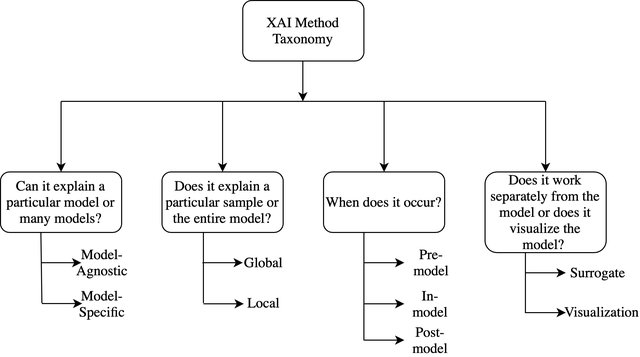
\includegraphics[width=.6\textwidth]{taxonomy}
%%     \caption{\footnotesize Singh et al, Explainable Deep Learning Models in Medical Image
%%       Analysis, Journal of Imaging 6(6):52, 2020}
%%   \end{figure}
%%   %% \begin{itemize}
%%   %% \item Εγγενής (intrisic) ερμηνευσιμότητα ή Post-hoc ερμηνεία;
%%   %% \item Τύπος ερμηνείας;
%%   %%   \begin{itemize}
%%   %%     \item Περιγραφικά στατιστικά για κάθε χαρ/κό, διάγραμμα επίδρασης
%%   %%       χαρ/κών, βάρη μοντέλου, δείγμα εισόδου (counterfactual), κλπ
%%   %%   \end{itemize}
%%   %% \item Γενική μέθοδος ή για συγκεκριμένο μοντέλο;
%%   %% \item Τοπική (local) ή ολική (global);
%%   %% \end{itemize}
%% \end{frame}

\end{document}
